\documentclass{report}
%%%%%%%%%%%%%% preamble.tex %%%%%%%%%%%%%%
\usepackage[T1]{fontenc}
\usepackage{etoolbox}
% Page Setup
\usepackage[letterpaper, tmargin=2cm, rmargin=0.5in, lmargin=0.5in, bmargin=80pt, footskip=.2in]{geometry}
\usepackage{adjustbox}
\usepackage{graphicx}
\usepackage{tikz}
\usepackage{mathrsfs}
\usepackage{mdframed}

% Create a new toggle
\newtoggle{firstsection}

% Redefine the \chapter command to reset the toggle for each new chapter
\let\oldchapter\chapter
\renewcommand{\chapter}{\toggletrue{firstsection}\oldchapter}

% Redefine the \section command to check the toggle
\let\oldsection\section
\renewcommand{\section}{
    \iftoggle{firstsection}
    {\togglefalse{firstsection}} % If it's the first section, just switch off the toggle for next sections
    {\clearpage} % If it's not the first section, start a new page
    \oldsection
}

% Abstract Design

\usepackage{lipsum}

\renewenvironment{abstract}
 {% Start of environment
  \quotation
  \small
  \noindent
  \rule{\linewidth}{.5pt} % Draw the rule to match the linewidth
  \par\smallskip
  {\centering\bfseries\abstractname\par}\medskip
 }
 {% End of environment
  \par\noindent
  \rule{\linewidth}{.5pt} % Ensure the closing rule also matches
  \endquotation
 }

% Mathematics
\usepackage{amsmath,amsfonts,amsthm,amssymb,mathtools}
\usepackage{xfrac}
\usepackage[makeroom]{cancel}
\usepackage{enumitem}
\usepackage{nameref}
\usepackage{multicol,array}
\usepackage{tikz-cd}
\usepackage{array}
\usepackage{multirow}% http://ctan.org/pkg/multirow
\usepackage{graphicx}

% Colors
\usepackage[dvipsnames]{xcolor}
\definecolor{myg}{RGB}{56, 140, 70}
\definecolor{myb}{RGB}{45, 111, 177}
\definecolor{myr}{RGB}{199, 68, 64}
% Define more colors here...
\definecolor{olive}{HTML}{6B8E23}
\definecolor{orange}{HTML}{CC5500}
\definecolor{brown}{HTML}{8B4513}
% Hyperlinks
\usepackage{bookmark}
\usepackage[colorlinks=true,linkcolor=blue,urlcolor=blue,citecolor=blue,anchorcolor=blue]{hyperref}
\usepackage{xcolor}
\hypersetup{
    colorlinks,
    linkcolor={red!50!black},
    citecolor={blue!50!black},
    urlcolor={blue!80!black}
}

% Text-related
\usepackage{blindtext}
\usepackage{fontsize}
\changefontsize[14]{14}
\setlength{\parindent}{0pt}
\linespread{1.2}

% Theorems and Definitions
\usepackage{amsthm}
\renewcommand\qedsymbol{$\blacksquare$}

% Define a new theorem style
\newtheoremstyle{mytheoremstyle}% name
  {}% Space above
  {}% Space below
  {}% Body font
  {}% Indent amount
  {\bfseries}% Theorem head font
  {.}% Punctuation after theorem head
  {.5em}% Space after theorem head
  {}% Theorem head spec (can be left empty, meaning ‘normal’)

% Apply the new theorem style to theorem-like environments
\theoremstyle{mytheoremstyle}

\newtheorem{theorem}{Theorem}[section]  
\newtheorem{definition}[theorem]{Definition} 
\newtheorem{lemma}[theorem]{Lemma}  
\newtheorem{corollary}[theorem]{Corollary}
\newtheorem{axiom}[theorem]{Axiom}
\newtheorem{example}[theorem]{Example}
\newtheorem{equiv_def}[theorem]{Equivalent Definition}

% tcolorbox Setup
\usepackage[most,many,breakable]{tcolorbox}
\tcbuselibrary{theorems}

% Define custom tcolorbox environments here...

%================================
% EXAMPLE BOX
%================================
% After you have defined the style and other theorem environments
\definecolor{myexamplebg}{RGB}{245, 245, 245} % Very light grey for background
\definecolor{myexamplefr}{RGB}{120, 120, 120} % Medium grey for frame
\definecolor{myexampleti}{RGB}{60, 60, 60}    % Darker grey for title

\newtcbtheorem[]{Example}{Example}{
    colback=myexamplebg,
    breakable,
    colframe=myexamplefr,
    coltitle=myexampleti,
    boxrule=1pt,
    sharp corners,
    detach title,
    before upper=\tcbtitle\par\vspace{-20pt}, % Reduced the space after the title
    fonttitle=\bfseries,
    description font=\mdseries,
    separator sign none,
    description delimiters={}{}, % No delimiters around the title
}{ex}
%================================
% Solution BOX
%================================
\makeatletter
\newtcolorbox{solution}{enhanced,
	breakable,
	colback=white,
	colframe=myg!80!black,
	attach boxed title to top left={yshift*=-\tcboxedtitleheight},
	title=Solution,
	boxed title size=title,
	boxed title style={%
			sharp corners,
			rounded corners=northwest,
			colback=tcbcolframe,
			boxrule=0pt,
		},
	underlay boxed title={%
			\path[fill=tcbcolframe] (title.south west)--(title.south east)
			to[out=0, in=180] ([xshift=5mm]title.east)--
			(title.center-|frame.east)
			[rounded corners=\kvtcb@arc] |-
			(frame.north) -| cycle;
		},
}
\makeatother

% %================================
% % Question BOX
% %================================
\makeatletter
\newtcbtheorem{question}{Question}{enhanced,
	breakable,
	colback=white,
	colframe=myb!80!black,
	attach boxed title to top left={yshift*=-\tcboxedtitleheight},
	fonttitle=\bfseries,
	title={#2},
	boxed title size=title,
	boxed title style={%
			sharp corners,
			rounded corners=northwest,
			colback=tcbcolframe,
			boxrule=0pt,
		},
	underlay boxed title={%
			\path[fill=tcbcolframe] (title.south west)--(title.south east)
			to[out=0, in=180] ([xshift=5mm]title.east)--
			(title.center-|frame.east)
			[rounded corners=\kvtcb@arc] |-
			(frame.north) -| cycle;
		},
	#1
}{question}
\makeatother

%%%%%%%%%%%%%%%%%%%%%%%%%%%%%%%%%%%%%%%%%%%
% TABLE OF CONTENTS
%%%%%%%%%%%%%%%%%%%%%%%%%%%%%%%%%%%%%%%%%%%


\usepackage{tikz}
\definecolor{doc}{RGB}{0,60,110}
\usepackage{titletoc}
\contentsmargin{0cm}
\titlecontents{chapter}[14pc]
{\addvspace{30pt}%
	\begin{tikzpicture}[remember picture, overlay]%
		\draw[fill=doc!60,draw=doc!60] (-7,-.1) rectangle (-0.9,.5);%
		\pgftext[left,x=-5.5cm,y=0.2cm]{\color{white}\Large\sc\bfseries Chapter\ \thecontentslabel};%
	\end{tikzpicture}\color{doc!60}\large\sc\bfseries}%
{}
{}
{\;\titlerule\;\large\sc\bfseries Page \thecontentspage
	\begin{tikzpicture}[remember picture, overlay]
		\draw[fill=doc!60,draw=doc!60] (2pt,0) rectangle (4,0.1pt);
	\end{tikzpicture}}%
\titlecontents{section}[3.7pc]
{\addvspace{2pt}}
{\contentslabel[\thecontentslabel]{3pc}}
{}
{\hfill\small \thecontentspage}
[]
\titlecontents*{subsection}[3.7pc]
{\addvspace{-1pt}\small}
{}
{}
{\ --- \small\thecontentspage}
[ \textbullet\ ][]

\makeatletter
\renewcommand{\tableofcontents}{
	\chapter*{%
	  \vspace*{-20\p@}%
	  \begin{tikzpicture}[remember picture, overlay]%
		  \pgftext[right,x=15cm,y=0.2cm]{\color{doc!60}\Huge\sc\bfseries \contentsname};%
		  \draw[fill=doc!60,draw=doc!60] (13,-.75) rectangle (20,1);%
		  \clip (13,-.75) rectangle (20,1);
		  \pgftext[right,x=15cm,y=0.2cm]{\color{white}\Huge\sc\bfseries \contentsname};%
	  \end{tikzpicture}}%
	\@starttoc{toc}}
\makeatother

\newcommand{\liff}{\llap{$\iff$}}
\newcommand{\rap}[1]{\rrap{\text{ (#1)}}}
\newcommand{\red}[1]{\textcolor{red}{#1}}
\newcommand{\blue}[1]{\textcolor{blue}{#1}}
\newcommand{\vi}[1]{\textcolor{violet}{#1}}
\newcommand{\olive}[1]{\textcolor{olive}{#1}}
\newcommand{\teal}[1]{\textcolor{teal}{#1}}
\newcommand{\brown}[1]{\textcolor{brown}{#1}}
\newcommand{\orange}[1]{\textcolor{orange}{#1}}
\newcommand{\tCaC}{\text{ \CaC }}
\newcommand{\CaC}{\red{CaC} }
\newcommand{\As}[1]{Assume \red{#1}}
\newcommand{\vdone}{\vi{\text{ (done) }}}
\newcommand{\bdone}{\blue{\text{ (done) }}}
\newcommand{\tdone}{\teal{\text{ (done) }}}
\newcommand{\odone}{\olive{\text{ (done) }}}
\newcommand{\bodone}{\brown{\text{ (done) }}}
\newcommand{\ordone}{\orange{\text{ (done) }}}
\newcommand{\ld}{\lambda}
\newcommand{\vecta}[1]{\textbf{#1}}
\newcommand{\set}[1]{\left\{ #1 \right\}}
\newcommand{\bset}[1]{\Big\{ #1 \Big\}}
\newcommand{\inR}{\in\R}
\newcommand{\inn}{\in\N}
\newcommand{\inz}{\in\Z}
\newcommand{\inr}{\in\R}
\newcommand{\inc}{\in\C}
\newcommand{\inq}{\in\Q}
\newcommand{\norm}[1]{\| #1 \|}
\newcommand{\bnorm}[1]{\Big\| #1 \Big\|}
\newcommand{\gen}[1]{\langle #1 \rangle}
\newcommand{\abso}[1]{\left|#1\right|}
\newcommand{\myref}[2]{\hyperref[#2]{#1\ \ref*{#2}}}
\newcommand{\customref}[2]{\hyperref[#1]{#2}}
\newcommand{\power}[1]{\mathcal{P}(#1)}
\newcommand{\dcup}{\mathbin{\dot{\cup}}}
\newcommand{\diam}[1]{\text{diam}\, #1}
\newcommand{\at}{\Big|}
\newcommand{\quotient}{\diagup}
\let\originalphi\phi % Store the original \phi in \originalphi
\renewcommand{\phi}{\varphi} % Redefine \phi to \varphi
\newcommand{\pfi}{\originalphi} % Define \pfi to display the original \phi
\newcommand{\diota}{\dot{\iota}}
\newcommand{\Log}{\operatorname{Log}}
\newcommand{\id}{\text{\textbf{id}}}
\usepackage{amsmath}

\makeatletter
\NewDocumentCommand{\extp}{e{^}}{%
  \mathop{\mathpalette\extp@{#1}}\nolimits
}
\NewDocumentCommand{\extp@}{mm}{%
  \bigwedge\nolimits\IfValueT{#2}{^{\extp@@{#1}#2}}%
  \IfValueT{#1}{\kern-2\scriptspace\nonscript\kern2\scriptspace}%
}
\newcommand{\extp@@}[1]{%
  \mkern
    \ifx#1\displaystyle-1.8\else
    \ifx#1\textstyle-1\else
    \ifx#1\scriptstyle-1\else
    -0.5\fi\fi\fi
  \thinmuskip
}
\makeatletter
\usepackage{pifont}
\makeatletter
\newcommand\Pimathsymbol[3][\mathord]{%
  #1{\@Pimathsymbol{#2}{#3}}}
\def\@Pimathsymbol#1#2{\mathchoice
  {\@Pim@thsymbol{#1}{#2}\tf@size}
  {\@Pim@thsymbol{#1}{#2}\tf@size}
  {\@Pim@thsymbol{#1}{#2}\sf@size}
  {\@Pim@thsymbol{#1}{#2}\ssf@size}}
\def\@Pim@thsymbol#1#2#3{%
  \mbox{\fontsize{#3}{#3}\Pisymbol{#1}{#2}}}
\makeatother
% the next two lines are needed to avoid LaTeX substituting upright from another font
\input{utxmia.fd}
\DeclareFontShape{U}{txmia}{m}{n}{<->ssub * txmia/m/it}{}
% you may also want
\DeclareFontShape{U}{txmia}{bx}{n}{<->ssub * txmia/bx/it}{}
% just in case
%\DeclareFontShape{U}{txmia}{l}{n}{<->ssub * txmia/l/it}{}
%\DeclareFontShape{U}{txmia}{b}{n}{<->ssub * txmia/b/it}{}
% plus info from Alan Munn at https://tex.stackexchange.com/questions/290165/how-do-i-get-a-nicer-lambda?noredirect=1#comment702120_290165
\newcommand{\pilambdaup}{\Pimathsymbol[\mathord]{txmia}{21}}
\renewcommand{\lambda}{\pilambdaup}
\renewcommand{\tilde}{\widetilde}
\DeclareMathOperator*{\esssup}{ess\,sup}
\newcommand{\bluecheck}{}%
\DeclareRobustCommand{\bluecheck}{%
  \tikz\fill[scale=0.4, color=blue]
  (0,.35) -- (.25,0) -- (1,.7) -- (.25,.15) -- cycle;%
}


\usepackage{tikz}
\newcommand*{\DashedArrow}[1][]{\mathbin{\tikz [baseline=-0.25ex,-latex, dashed,#1] \draw [#1] (0pt,0.5ex) -- (1.3em,0.5ex);}}

\newcommand{\C}{\mathbb{C}}	
\newcommand{\F}{\mathbb{F}}
\newcommand{\N}{\mathbb{N}}
\newcommand{\Q}{\mathbb{Q}}
\newcommand{\R}{\mathbb{R}}
\newcommand{\Z}{\mathbb{Z}}



\title{\Huge{HWs}}
\author{\huge{Eric Liu}}
\date{}
\begin{document}
\maketitle
\newpage% or \cleardoublepage
% \pdfbookmark[<level>]{<title>}{<dest>}
\pdfbookmark[section]{\contentsname}{toc}
\tableofcontents
\pagebreak

\chapter{General Analysis HW}
\section{Brunn-Minkowski Inequality}
\begin{abstract}
  This HW assignment require us to prove the Brunn-Minkowski Inequality. Note that in this HW, we use bold face $\textbf{x}$ to denote $(x_1,\dots ,x_d)$ element of $\R^d$. Also, throughout this HW, we shall suppose $\abso{A}>0$ and $\abso{A},\abso{B}<\infty$; otherwise, the proof would be trivial. 
\end{abstract}
\begin{mdframed}
  We first introduce some notation. Given two sets $A,B\subseteq \R^d$ and a point $\textbf{x}\inr^d$, we write 
\begin{align*}
A+\textbf{x}\triangleq \set{\textbf{a}+\textbf{x}\inr^d: \textbf{a} \in A}
\end{align*}
and write 
\begin{align*}
A+B \triangleq \set{\textbf{a}+\textbf{b} \inr^d: \textbf{a}\in A\text{ and }\textbf{b} \in  B}
\end{align*}
Note that elementary set theory tell us 
\begin{align}
\label{trans}
  (A+\textbf{x})+(B+\textbf{y})=(A+B)+(\textbf{x}+\textbf{y})
\end{align}
\end{mdframed}
\begin{theorem}
\label{Brunn-Minkowski Inequality for Bricks}
\textbf{(Brunn-Minkowski Inequality for rectangles)} Suppose $A,B$ are two  \textbf{rectangles}, i.e., $A$ is of the form $\prod_{j=1}^d[x_j,y_j]$, and so is $B$. We have 
\begin{align*}
\abso{A}^{\frac{1}{d}}+ \abso{B}^{\frac{1}{d}}\leq \abso{A+B}^{\frac{1}{d}}
\end{align*}
\end{theorem}
\begin{proof}
Because Lebesgue measure is translation invariant, by  \myref{Equation}{trans}, we can WLOG suppose 
\begin{align*}
A=\prod_{j=1}^d [0,a_j]\text{ and }B=\prod_{j=1}^d [0,b_j]
\end{align*}
It is clear that 
\begin{align*}
A+B= \prod_{j=1}^d [0,a_j+b_j]
\end{align*}
By direct computation, we know that 
\begin{align*}
\abso{A+B}=\prod_{j=1}^d (a_j+b_j)\text{ and }\abso{A}=\prod_{j=1}^d a_j\text{ and }\abso{B}=\prod_{j=1}^d b_j
\end{align*}
Then by AM-GM inequality, we have 
\begin{align*}
\frac{\abso{A}^{\frac{1}{d}}}{\abso{A+B}^{\frac{1}{d}}}=\Big(\prod_{j=1}^d \frac{a_j}{a_j+b_j}\Big)^{\frac{1}{d}}\leq \frac{1}{d}\sum_{j=1}^d \frac{a_j}{a_j+b_j}
\end{align*}
Similarly, by AM-GM inequality, we have
\begin{align*}
\frac{\abso{B}^{\frac{1}{d}}}{\abso{A+B}^{\frac{1}{d}}}=\Big(\prod_{j=1}^d \frac{b_j}{a_j+b_j}\Big)^{\frac{1}{d}}\leq \frac{1}{d}\sum_{j=1}^d \frac{b_j}{a_j+b_j}
\end{align*}
Adding two inequalities together, we now have 
\begin{align*}
\frac{\abso{A}^{\frac{1}{d}}+\abso{B}^{\frac{1}{d}}}{\abso{A+B}^{\frac{1}{d}}}\leq \frac{1}{d}\sum_{j=1}^d \frac{a_j+b_j}{a_j+b_j}=1
\end{align*}
The result then follows from multiplying both side with $\abso{A+B}^{\frac{1}{d}}$. 
\end{proof}
\begin{theorem}
\label{BMIb}
\textbf{(Brunn-Minkowski Inequality for finite union of non-overlapping of rectangles)} Suppose $A$ is a union of a finite collection of non-overlapping rectangles, and the same holds for $B$. We have 
 \begin{align*}
\abso{A}^{\frac{1}{d}}+ \abso{B}^{\frac{1}{d}}\leq \abso{A+B}^{\frac{1}{d}}
\end{align*}
\end{theorem}
\begin{proof}
We prove by induction on $k$, the sum of the rectangles in $A$ and $B$. The base case $k=2$ have been proved by \myref{Theorem}{Brunn-Minkowski Inequality for Bricks}.  Suppose the proposition hold true when $k\leq r$. Let $k=r+1$. Because the rectangles in $A$ are non-overlapping, by a translation and renaming axis if necessary, we can suppose the following proposition.
\begin{center}
   \begin{minipage}{0.9\linewidth}  
     $\vspace{0.05cm}$\\
     Proposition 1: Both $A^+\triangleq A\cap \set{\textbf{x}\inr^d: x_1\geq 0}$ and $A^-\triangleq A\cap \set{\textbf{x}\inr^d: x_1\leq 0}$ are unions of a finite collection of non-overlapping rectangles, with each collection containing at least one fewer rectangle than $A$. \label{pp1}\\ 
   \end{minipage}
\end{center}

\customref{pp1}{Proposition 1} holds because, if we write $A=A_1\cup \cdots \cup A_m$, where $A_1,\dots , A_m$ are non-overlapping rectangles, then by translation and remaining axis, we can suppose that $A_1,A_2$ lie in distinct closed subspace, either $\set{\textbf{x}\inr^d:x_1\geq 0}$ or $\set{\textbf{x}\inr^d:x_1\leq 0}$, while for all $n\geq 3$, $A_n \cap \set{\textbf{x}\inr^d: x_1\geq 0}$ is either empty or also a rectangle.\\

Note that $h:\R\rightarrow \R$ defined by
\begin{align*}
h(t)\triangleq  \abso{\Big(B+(t,0,\dots ,0) \Big)\cap \set{\textbf{x}\inr^d: x_1\geq 0}}
\end{align*}
is clearly an increasing continuous function such that 
\begin{align*}
h(-M)=0\text{ and }h(M)=\abso{B}\text{ for some }M>0
\end{align*}
Then by IVT, we can translate $B$ to let $B$ satisfy 
\begin{align}
  \label{rai}
\frac{\abso{B^+}}{\abso{B}}=\frac{\abso{A^+}}{\abso{A}} \text{ where }B^+ \triangleq B \cap \set{\textbf{x}\inr^d: x_1\geq 0}
\end{align}
Define $B^- \triangleq B \cap \set{\textbf{x} \in \mathbb{R}^d : x_1 \leq 0}$. With reasoning similar to that of \customref{pp1}{Proposition 1}, we know that $B^+$ and $B^-$ are both unions of collections of non-overlapping rectangles, with each collection consisting of no more rectangles than $B$. Therefore, by \customref{pp1}{Proposition 1}, we can deduce that the sum of the number of rectangles in $A^+$ and $B^+$ is at least one fewer than $r + 1$, and the same holds for the sum of the number of rectangles in $A^-$ and $B^-$. Then, because the proposition holds true for $k \leq r$, we now have
\begin{align*}
\abso{A^+}^{\frac{1}{d}}+ \abso{B^+}^{\frac{1}{d}}\leq \abso{A^++B^+}^{\frac{1}{d}}\text{ and }\abso{A^-}^{\frac{1}{d}}+ \abso{B^-}^{\frac{1}{d}}\leq \abso{A^-+B^-}^{\frac{1}{d}}
\end{align*}
Note that for each $\textbf{x}$ in the interior of $A^++B^+$, we must have  $x_1>0$, and for each  $\textbf{y}$ in the interior of $A^-+B^-$, we must have $y_1<0$. This implies that  $(A^++B^+)$ and $(A^-+B^-)$ are non-overlapping. Now, because 
\begin{align*}
A+B =(A^++B^+)\cup (A^-+B^-)
\end{align*}
if we define $\rho \triangleq \frac{\abso{A^+}}{\abso{A}}$, from \myref{Equation}{rai} we can finally deduce 
\begin{align*}
\abso{A+B}&= \abso{A^++B^+}+ \abso{A^-+B^-}\\
&\geq \Big(\abso{A^+}^{\frac{1}{d}} + \abso{B^+}^{\frac{1}{d}} \Big)^{d} + \Big(\abso{A^-}^{\frac{1}{d}}+\abso{B^-}^{\frac{1}{d}}  \Big)^d \\ 
(\because \frac{\abso{A^-}}{\abso{A}}=\frac{\abso{B^-}}{\abso{B}}=1-\rho)\hspace{0.5cm}&=\Big((\rho \abso{A})^{\frac{1}{d}}+ (\rho \abso{B})^{\frac{1}{d}} \Big)^d + \Big(((1-\rho)\abso{A})^{\frac{1}{d}}+ ((1-\rho)\abso{B})^{\frac{1}{d}} \Big)^d \\
&=(\abso{A}^{\frac{1}{d}}+\abso{B}^{\frac{1}{d}})^d
\end{align*}
which give us the desired inequality  
\begin{align*}
\abso{A+B}^{\frac{1}{d}}\geq \abso{A}^{\frac{1}{d}}+ \abso{B}^{\frac{1}{d}}
\end{align*}
\end{proof}
\begin{theorem}
\label{BMIo}
\textbf{(Brunn-Minkowski Inequality for bounded open set)} Suppose $A,B$ are both bounded open subset of  $\R^d$. We have 
 \begin{align*}
\abso{A}^{\frac{1}{d}}+ \abso{B}^{\frac{1}{d}}\leq \abso{A+B}^{\frac{1}{d}}
\end{align*}
\end{theorem}
\begin{proof}
Note that  $A+B$ is open since it is a union of the open sets:
\begin{align*}
A+B=\bigcup_{\textbf{b}\in B}A+\textbf{b}\text{ }
\end{align*}
It follows that $A+B$ is Lebesgue measurable, so it makes sense for us to write  $\abso{A+B}$. By a proposition taught in class, we can let 
\begin{align*}
A=\bigcup_{n\inn}K_{n,a}\text{ and }B=\bigcup_{n\inn}K_{n,b}
\end{align*}
where $(K_{n,a})$ are non-overlapping rectangles, and so are $(K_{n,b})$. It is clear that  
\begin{align*}
  \Big(\bigcup_{n=1}^N K_{n,a} \Big) + \Big(\bigcup_{n=1}^N K_{n,b} \Big) \nearrow A+B\text{ as }N \to \infty
\end{align*}
This together with \myref{Theorem}{BMIb} give us the desired inequality  
\begin{align*}
\abso{A+B}^{\frac{1}{d}}&=\lim_{N\to \infty} \abso{\Big(\bigcup_{n=1}^N K_{n,a} \Big) + \Big( \bigcup_{n=1}^N K_{n,b}  \Big)}^{\frac{1}{d}}\\
&\geq \lim_{N\to \infty} \abso{\bigcup_{n=1}^N K_{n,a}}^{\frac{1}{d}}+ \abso{\bigcup_{n=1}^N K_{n,b}}^{\frac{1}{d}}=\abso{A}^{\frac{1}{d}}+\abso{B}^{\frac{1}{d}}
\end{align*}
\end{proof}
\begin{theorem}
\label{BMIc}
\textbf{(Brunn-Minkowski Inequality for compact set)} Suppose $A,B$ are both compact subset of  $\R^d$. We have 
 \begin{align*}
\abso{A}^{\frac{1}{d}}+ \abso{B}^{\frac{1}{d}}\leq  \abso{A+B}^{\frac{1}{d}}
\end{align*}
\end{theorem}
\begin{proof}
For each $\epsilon >0$, define 
\begin{align*}
A_{\epsilon }\triangleq \set{\textbf{x}\inr^d: d(\textbf{x},A)<\epsilon }\text{ and }B_{\epsilon }\triangleq \set{\textbf{x}\inr^d: d(\textbf{x},B)<\epsilon }
\end{align*}
To see $A_\epsilon $ is open, observe that if $\textbf{x}\in A_{\epsilon }$, then for all $\textbf{y}$ in the open ball $\set{\textbf{y}:d(\textbf{x},\textbf{y})<\frac{\epsilon -d(\textbf{x},A)}{2}}$ centering $\textbf{x}$, we can pick some $\textbf{z} \in A$ satisfying $d(\textbf{x},\textbf{z})< d(\textbf{x},A) + \frac{\epsilon}{2}$ to have
\begin{align*}
  d(\textbf{y},A)&\leq d(\textbf{y},\textbf{z})\\
  &\leq d(\textbf{x},\textbf{z})+d(\textbf{x},\textbf{y})\\
  &\leq d(\textbf{x},\textbf{z})+ \frac{\epsilon -d(\textbf{x},A)}{2}\\
  &\leq d(\textbf{x},\textbf{z})-d(\textbf{x},A)+ \frac{\epsilon }{2}<\epsilon \text{ implying }\textbf{y} \in A_\epsilon 
\end{align*}
Similar argument shows that $B_{\epsilon }$ are open. To see $A_\epsilon \searrow A$, note that for all $\textbf{x}\not\in A$, because $d(\textbf{x},\textbf{z})$ is a function continuous in the variable $\textbf{z}$ and $A$ is compact, by EVT we have 
 \begin{align*}
d(\textbf{x},A)=d(\textbf{x},\textbf{z})>0\text{ for some $\textbf{z}\in A$ }
\end{align*}
where the inequality holds because $\textbf{z}\in A \implies \textbf{x}\neq \textbf{z} $. Similar argument shows that $B_\epsilon \searrow B$. We now prove 
\begin{align}
\label{A+B}
A+B= \lim_{\epsilon \to 0} A_\epsilon +B_ \epsilon 
\end{align}
It is clear that 
\begin{align}
\label{a+b}
A+B\subseteq \bigcap_{\epsilon >0}A_\epsilon +B_\epsilon 
\end{align}
Fix an arbitrary $\textbf{z}\in \bigcap_{\epsilon >0}A_\epsilon +B_\epsilon $. For all $n\inn$, by definition there exists $\textbf{a}_n \in A_{\frac{1}{n}} $ and $\textbf{b}_n \in B_{\frac{1}{n}} $ such that $\textbf{z}=\textbf{a}_n+\textbf{b}_n$. By the Bolzano-Weierstrass Theorem, there exists convergent subsequence $\textbf{a}_{n_k}$. Applying Bolzano-Weierstrass Theorem again, we find that there exists convergent subsequence $\textbf{b}_{n_{k_j}}$. Clearly, $\textbf{a}_{n_{k_j}}$ also converge. For brevity, we denote these subsequences simply by $\textbf{a}_{n_k}$ and $\textbf{b}_{n_k}$, and we denote their limit by 
\begin{align*}
\textbf{a}=\lim_{k\to \infty}\textbf{a}_{n_k}\text{ and }\textbf{b}=\lim_{k\to \infty}\textbf{b}_{n_k}
\end{align*}
We now shows that 
\begin{align*}
 \textbf{a}\in A
\end{align*}
Assume $\textbf{a} \not\in A$ for a contradiction. By EVT, $d(\textbf{a},A)=d(\textbf{a},\textbf{a}')$ for some $\textbf{a}'\in A$. Note that $d(\textbf{a},\textbf{a}')>0$ because $\textbf{a}\not\in A\implies \textbf{a}\neq \textbf{a}'$. We have shown $d(\textbf{a},A)=d(\textbf{a},\textbf{a}')>0$. \\

Let $m$ be large enough so that $\frac{1}{n_m}< \frac{d(\textbf{a},A)}{2}$. Since $d(\textbf{a}_{n_m},A)< \frac{1}{n_m}< \frac{d(\textbf{a},A)}{2}$, we can select $\textbf{a}'' \in A$ such that $d(\textbf{a}_{n_m},\textbf{a}'')< \frac{d(\textbf{a},A)}{2}$. This give us 
\begin{align*}
d(\textbf{a},A)\leq d(\textbf{a},\textbf{a}'')\leq d(\textbf{a},\textbf{a}_{n_m})+ d(\textbf{a}_{n_m},\textbf{a}'')< \frac{d(\textbf{a},A)}{2}+ \frac{d(\textbf{a},A)}{2}
\end{align*}
This results in $d(\textbf{a}, A) < d(\textbf{a}, A)$, a contradiction. We have proved $\textbf{a} \in A$. Similar arguments shows that $\textbf{b} \in B$. \\

Now, since $\textbf{z}=\textbf{a}_{n_k}+\textbf{b}_{n_k}$ for all $k$, we see 
\begin{align*}
\textbf{z}=\lim_{k\to \infty}\textbf{a}_{n_k}+\textbf{b}_{n_k}=\lim_{k\to \infty}\textbf{a}_{n_k}+\lim_{k\to \infty}\textbf{b}_{n_k}=\textbf{a}+\textbf{b} \in A+B
\end{align*}
Because $\textbf{z}$ is arbitrarily selected from $\bigcap_{\epsilon >0}A_\epsilon +B_\epsilon $. We have in fact proved 
\begin{align*}
\bigcap_{\epsilon >0}A_\epsilon +B_\epsilon  \subseteq A+B
\end{align*}
which together with \myref{Equation}{a+b} implies \myref{Equation}{A+B}. With \myref{Equation}{A+B} established, we can now apply  \myref{Theorem}{BMIo} to have the desired inequality 
\begin{align*}
  \abso{A+B}^{\frac{1}{d}}&=\Big(\lim_{\epsilon \to 0} \abso{A_\epsilon +B_\epsilon}  \Big)^{\frac{1}{d}}\\
  &=\lim_{\epsilon \to 0}\abso{A_\epsilon +B_\epsilon }^{\frac{1}{d}}\\
  &\geq \lim_{\epsilon \to 0}\abso{A_\epsilon }^{\frac{1}{d}}+ \abso{B_\epsilon }^{\frac{1}{d}}= \abso{A}^{\frac{1}{d}}+ \abso{B}^{\frac{1}{d}}
\end{align*}
\end{proof}
\begin{mdframed}
Before we proceed to develop the remaining Brunn-Minkowski Inequality, we first have to prove that Lebesgue measure is  \textbf{inner regular}. 
\end{mdframed}
\begin{theorem}
\label{Lmi}
\textbf{(Lebesgue measure is inner regular)} If $A\subseteq \R^d$ is Lebesgue measurable, then 
\begin{align*}
\abso{A}=\sup \set{\abso{K}:K\text{ is some compact subset of  }A}
\end{align*}
\end{theorem}
\begin{proof}
Because $A$ is measurable, we know $A\cap \overline{B_n(\textbf{0})}$ is measurable for all $n\inn$. Therefore, for all $n\inn$, $(A\cap \overline{B_n(\textbf{0})})^c$ is measurable. Then by definition, there exists open $O_n$ containing $(A\cap \overline{B_n(\textbf{0})})^c$,  such that $\abso{O_n\setminus (A\cap B_n(\textbf{0}))^c }< \frac{1}{n}$. Now, for each $n\inn$, define closed set $K_n\triangleq O_n^c$. We then have 
\begin{align*}
  K_n \subseteq A\cap \overline{B_n(\textbf{0})}
\end{align*}
and 
\begin{align*}
  (A\cap \overline{B_n(\textbf{0})}) \setminus K_n= A\cap \overline{B_n(\textbf{0})}\cap O_n=O_n \setminus (A\cap B_n(\textbf{0}))^c
\end{align*}
This then give us 
\begin{align*}
\abso{(A\cap  \overline{B_n(\textbf{0})})\setminus K_n}=\abso{O_n\setminus (A\cap B_n(\textbf{0}))^c }< \frac{1}{n}
\end{align*}
Note that because $K_n \subseteq B_n(\textbf{0})$ is bounded and closed, by Hiene-Borel, we know $K_n$ is compact. Lastly, to close out the proof, we are required to show $\abso{K_n}\to \abso{A}$ as $n \to \infty$. Note that $\abso{A\cap \overline{B_n(\textbf{0}})}\nearrow \abso{A}$ as $n\to \infty$  because $A\cap \overline{B_n(\textbf{0})}\nearrow A$ as $n\to \infty$. Then because $\abso{A\cap \overline{B_n(\textbf{0})}}\geq \abso{K_n}\geq \abso{A\cap \overline{ B_n(\textbf{0})}}- \frac{1}{n}$, we see that $\abso{K_n}\to \abso{A}$ by squeeze Theorem. 
\end{proof}
\begin{theorem}
\textbf{(Brunn-Minkowski Inequality for measurable set)} Suppose $A,B$ are measurable subset of  $\R^d$ and $A+B$ is also measurable. We have 
 \begin{align*}
\abso{A}^{\frac{1}{d}}+ \abso{B}^{\frac{1}{d}}\leq \abso{A+B}^{\frac{1}{d}}
\end{align*}
\end{theorem}
\begin{proof}
Because \customref{lmi}{Lebesgue measure is inner regular} and $A,B$ are of finite measure, for each $n\inn$, we can let $A_n,B_n$ each be compact subset of  $A,B$ such that $\abso{A}-\abso{A_n}<\frac{1}{n}$  and $\abso{B}-\abso{B_n}<\frac{1}{n}$. It then follows from \myref{Theorem}{BMIc} that 
\begin{align*}
\abso{A+B}^{\frac{1}{d}}\geq \lim_{n\to \infty}\abso{A_n+B_n}^{\frac{1}{d}}\geq \lim_{n\to \infty} \abso{A_n}^{\frac{1}{d}}+ \abso{B_n}^{\frac{1}{d}}=\abso{A}^{\frac{1}{d}}+ \abso{B}^{\frac{1}{d}}
\end{align*}
\end{proof}
\section{HW1}
\begin{question}{}{}
Show $\R^n$ is complete.
\end{question}
\begin{proof}
Let $\textbf{x}_k$ be an arbitrary Cauchy sequence in $\R^n$. We are required to show  $\textbf{x}_k$ converge in $\R^n$. For each $k$, denote  $\textbf{x}_k$ by $(x_{(1,k)},\dots ,x_{(n,k)})$. We claim that for each $i \in \set{1,\dots ,n}$
\begin{align*}
x_{(i,k)}\text{ is a Cauchy sequence }
\end{align*}
Fix $i$ and $\epsilon >0$. To show $x_{(i,k)}$ is a Cauchy sequence, we are required to find $N\inn$ such that for all $r,m\geq N$ we have 
\begin{align*}
\abso{x_{(i,r)}-x_{(i,m)}}\leq \epsilon 
\end{align*}
Because $\textbf{x}_k$ is a Cauchy sequence in $\R^n$, we know there exists  $N\inn$ such that for all $r,m\geq N$, we have 
\begin{align*}
\abso{\textbf{x}_r-\textbf{x}_m}< \epsilon 
\end{align*}
Fix such $N$ and arbitrary $r,m\geq M$. Observe 
\begin{align*}
\abso{x_{(i,r)}-x_{(i,m)}}\leq \sqrt{\sum_{j=1}^n \abso{x_{(j,r)}-x_{(j,m)}}^2}= \abso{\textbf{x}_r - \textbf{x}_m}< \epsilon 
\end{align*}
We have proved that for each $i\in \set{1,\dots ,n}$, the real sequence $x_{(i,k)}$ is Cauchy. We now claim that for each $i \in \set{1,\dots, n}$, we have 
\begin{align*}
  \limsup_{r\to\infty} x_{(i,r)}\inr \text{ and }\lim_{k\to \infty}x_{(i,k)}= \limsup_{r\to\infty} x_{(i,r)}
\end{align*}
Again fix $i$. Because $x_{(i,k)}$ is a Cauchy sequence, we know there exists some $N$ such that for all $r,m\geq N$, we have 
 \begin{align*}
\abso{x_{(i,r)}-x_{(i,m)}}<1
\end{align*}
This implies that for all $r\geq N$, we have 
\begin{align}
x_{(i,r)}< x_{(i,N)}+1 \label{ran1}
\end{align}
\myref{Equation}{ran1} then tell us 
\begin{align*}
x_{(i,N)}+1\text{ is an upper bound of }\set{x_{(i,r)}:r\geq N}
\end{align*}
Then by definition of $\sup $, we have
\begin{align*}
\sup \set{x_{(i,r)}:r\geq N} \leq x_{(i,N)}+1 \inr
\end{align*}
This then implies $\limsup_{r\to\infty} x_{(i,r)}\inr$. We now prove 
\begin{align}
\label{ran2}
\lim_{k\to \infty}x_{(i,k)}= \limsup_{r\to\infty} x_{(i,r)}
\end{align}
Fix $\epsilon >0$. We are required to find $N$ such that
\begin{align*}
\forall k\geq N, \abso{x_{(i,k)}-\limsup_{r\to\infty}x_{(i,r)}} \leq \epsilon 
\end{align*}
Because $\set{x_{(i,k)}}_{k\inn}$ is a Cauchy sequence, we can let $N_0$ satisfy 
\begin{align*}
\forall k,m\geq N_0, \abso{x_{(i,k)}-x_{(i,m)}}<\frac{\epsilon}{2}
\end{align*}
Because $\sup \set{x_{(i,k)}:k\geq N'}\searrow \limsup_{r\to\infty} x_{(i,r)}$ as $N'\to \infty$, we know there exists $N_1>N_0$ such that 
 \begin{align*}
\limsup_{r\to\infty} x_{(i,r)}-\frac{\epsilon}{2} <\sup \set{x_{(i,k)}:k\geq N_0}\leq \limsup_{r\to\infty}  x_{(i,r)} + \frac{\epsilon}{2} 
\end{align*}
Then because $\limsup_{r\to\infty} x_{(i,r)}-\frac{\epsilon}{2}$ is strictly smaller than the smallest upper bound of $\set{x_{(i,k)}:k\geq N_1}$, we see $\limsup_{n\to\infty} x_{(i,r)}-\frac{\epsilon}{2}$ is not an upper bound of $\set{x_{(i,k)}:k\geq N_1}$. This implies the existence of some $N$ such that  $N\geq N_1$ and
\begin{align*}
\limsup_{r\to\infty} x_{(i,r)}-\frac{\epsilon}{2}< x_{(i,N)}\leq \limsup_{r\to\infty}x_{(i,r)} + \frac{\epsilon}{2}
\end{align*}
Now observe that for all $k\geq N$, because $N\geq N_1\geq N_0$ 
\begin{align*}
  \limsup_{r\to\infty} x_{(i,r)} - \epsilon <x_{(i,N)}-\frac{\epsilon}{2}<x_{(i,k)}< x_{(i,N)}+\frac{\epsilon}{2} \leq \limsup_{r\to\infty} x_{(i,r)} + \epsilon   
\end{align*}
This implies for all $k\geq N$, we have 
\begin{align*}
\abso{x_{(i,k)}-\limsup_{r\to\infty} x_{(i,r)}}\leq \epsilon 
\end{align*}
We have just proved \myref{Equation}{ran2}. Lastly, to close out the proof, we show 
\begin{align}
\label{ran3}
\lim_{k\to \infty}\textbf{x}_k = \Big(\lim_{k\to \infty}x_{(1,k)},\dots ,\lim_{k\to \infty}x_{(n,k)}\Big)
\end{align}
Fix $\epsilon >0$. For each $i \in \set{1,\dots ,n}$, let $N_i$ satisfy 
 \begin{align*}
  \forall r\geq N_i ,\abso{x_{(i,r)}- \lim_{k\to \infty}x_{(i,k)}}\leq  \frac{\epsilon }{\sqrt{n} }
\end{align*}
Observe that for all $r\geq \max_{i\in \set{1,\dots,n}} N_i$, we have 
\begin{align*}
\abso{\textbf{x}_r - \Big(\lim_{k\to \infty}x_{(1,k)},\dots ,\lim_{k\to \infty}x_{(n,k)} \Big)}&=\sqrt{\sum_{i=1}^n \abso{x_{(i,r)}- \lim_{k\to \infty}x_{(i,k)}}^2} \\
&\leq \sqrt{\sum_{i=1}^n \frac{\epsilon^2}{n}}=\epsilon 
\end{align*}
We have proved \myref{Equation}{ran3}.











\end{proof}
\begin{question}{}{}
Show $\Q$ is dense in $\R$. 
\end{question}
\begin{proof}
Fix $x\inr$ and $\epsilon >0$. To show $\Q$ is dense in  $\R$, we have to find $q\inq$ such that $\abso{x-q}<\epsilon $.\\

Let $m\inn$ satisfy $\frac{1}{m}<\epsilon $. Let $n$ be the largest integer such that $n\leq mx$. Because $n$ is the largest integer such that $n\leq mx$, we know $mx-n<1$, otherwise we can deduce $n+1\leq mx$, which is impossible, since $n+1$ is an integer and $n$ is the largest integer such that $n\leq mx$. We now see that 
\begin{align*}
\frac{n}{m}\inq \text{ and }\abso{x-\frac{n}{m}}=\frac{mx-n}{m}< \frac{1}{m}<\epsilon 
\end{align*}



\end{proof}
\begin{theorem}
\textbf{(Distance Formula)} Given two subsets $A,B$ of a metric space, we have 
\begin{align*}
d(A,B)= \inf_{b \in B}d(A,b)
\end{align*}
\end{theorem}
\begin{proof}
Fix arbitrary $b \in B$. It is clear that 
\begin{align*}
d(A,B)\leq d(A,b)
\end{align*}
It then follows $d(A,B)\leq \inf_{b \in B}d(A,b)$. Fix arbitrary $a \in A$ and $b_0 \in B$. Observe that 
\begin{align*}
d(a,b_0)\geq  d(A,b_0) \geq \inf_{b \in B}d(A,b)
\end{align*}
It then follows $\inf_{b \in B}d(A,b)\leq d(A,B)$. 
\end{proof}
\begin{question}{}{}
Let $E_1,E_2$ be non-empty sets in  $\R^n$ with $E_1$ closed and  $E_2$ compact. Show that there are points  $x_1\in E_1$ and $x_2 \in E_2$ such that 
\begin{align*}
d(E_1,E_2)=\abso{x_1-x_2}
\end{align*}
Deduce that $d(E_1,E_2)$ is positive if such $E_1,E_2$ are disjoint. 
\end{question}

\begin{proof}
Because 
\begin{enumerate}[label=(\alph*)]
  \item $f(x)\triangleq d (E_1,x)$ is a continuous function on $\R^n$. 
  \item $E_2$ is compact. 
\end{enumerate}
It now follows by EVT there exists some  $x_2 \in E_2$ such that 
\begin{align*}
d(E_1,x_2)=\min_{x \in E_2} d(E_1,x)=\inf_{x \in E_2}d(E_1,x)=d(E_1,E_2)
\end{align*}
where the last equality is proved above. We can now reduce the problem into finding $x_1$ in $E_1$ such that  
\begin{align*}
  \vi{d(x_1,x_2)=d(E_1,x_2)}
\end{align*}
For each $n\inn$, let $t_n$ satisfy 
 \begin{align*}
t_n \in E_1\text{ and }d(t_n,x_2)< d(E_1,x_2) + \frac{1}{n}
\end{align*}
Clearly, $t_n$ is a bounded sequence. Then by Bolzano-Weierstrass Theorem, there exists a convergence subsequence $t_{n_k}$. Now, because $E_1$ is closed, we know 
\begin{align*}
x_1\triangleq \lim_{k\to \infty}t_{n_k} \in E_1
\end{align*}
It then follows from the function $f(x)\triangleq d(x,x_2)$ being continuous on $\R^n$ such that 
 \begin{align*}
d(x_1,x_2)=\lim_{k\to \infty}d(t_{n,k},x_2)=d(E_1,x_2)
\end{align*}
\end{proof}
\begin{question}{}{}
Prove that the distance between two nonempty, compact, disjoint sets in $\R^n$ is positive. 
\end{question}
\begin{proof}
The proof follows from the result in last question while acknowledging compact is closed. 
\end{proof}
\begin{question}{}{}
Prove that if $f$ is continuous on $[a,b]$, then $f$ is Riemann-integrable on$[a,b]$. 
\end{question}
\begin{proof}
Let $\overline{\int_a^b}fdx$ and $\underline{\int_a^b}fdx$ respectively denote the upper and lower Darboux sums. We prove that 
\begin{align*}
\overline{\int_a^b}fdx=\underline{\int_a^b}fdx
\end{align*}
Fix $\epsilon $. We reduce the problem into proving the existence of some partition $\set{a=x_0,x_1,\dots ,x_n=b}$ such that  
\begin{align*}
  \sum_{i=1}^n \Big[M_i-m_i \Big](x_i-x_{i-1}) \leq \epsilon 
\end{align*}
where 
\begin{align*}
M_i\triangleq \sup_{t \in [x_{i-1},x_i]}f(t)\text{ and }m_i \triangleq \inf_{t \in [x_{i-1},x_i]}f(t)
\end{align*}
Because $f$ is continuous on the compact interval $[a,b]$, we know $f$ is uniformly continuous on $[a,b]$. Let $\delta$ satisfy 
\begin{align*}
\abso{x-y}< \delta \text{ and }x,y \in [a,b] \implies \abso{f(x)-f(y)}< \frac{\epsilon }{b-a}
\end{align*}
Let $n$ satisfy $\frac{b-a }{n}<\delta$. We claim the partition 
\begin{align*}
\set{a=x_0,x_1,\dots ,x_n=b}\text{ where }x_i\triangleq a+\frac{i(b-a)}{n}\text{ suffices }
\end{align*}
Now, by EVT, we know that for each $i$, there exists some  $t_{i,M},t_{i,m} \in [x_{i-1},x_i]$ such that 
\begin{align*}
f(t_{i,m})=m_i\text{ and }f(t_{i,M})=M_i
\end{align*}
Then because 
\begin{align*}
\abso{t_{i,m}-t_{i,M}}\leq x_i-x_{i-1}\leq \frac{b-a}{n}<\delta 
\end{align*}
We know $M_i-m_i< \frac{\epsilon}{b-a}$. This now give us 
\begin{align*}
  \sum_{i=1}^n \Big[M_i-m_i \Big](x_i-x_{i-1})&< \sum_{i=1}^n \frac{\epsilon }{(b-a)}(x_i-x_{i-1})\\
  &= \frac{\epsilon }{b-a}\sum_{i=1}^n (x_i-x_{i-1})\\
  &=\frac{\epsilon}{b-a}(b-a)=\epsilon 
\end{align*}



\end{proof}
\begin{question}{}{}
Find $\limsup_{n\to\infty} E_n$ and $\liminf_{n\to\infty} E_n$ where 
\begin{align*}
E_n\triangleq \begin{cases}
  [\frac{-1}{n},1]& \text{ if $n$ is odd }\\
  [-1,\frac{1}{n}]& \text{ if $n$ is even }
\end{cases}
\end{align*}
\end{question}
\begin{proof}
Fix arbitrary $n\inn$. Let $p,q\geq n$ respectively be odd and even. We see 
\begin{align*}
[0,1]\subseteq E_p \text{ and }[-1,0]\subseteq E_q
\end{align*}
This now implies 
\begin{align*}
[-1,1]\subseteq \bigcup_{k\geq n}E_k 
\end{align*}
Then because $n$ is arbitrary, it follows 
 \begin{align*}
\limsup_{n\to\infty} E_n=\bigcap_{n=1}^{\infty}\bigcup_{k\geq n} E_k = [-1,1]
\end{align*}
Again, fix arbitrary $n\inn$ and $\epsilon >0$. Let $p,q$ respectively be even and odd integers greater than  $\max \set{n,\frac{1}{\epsilon }}$. We now see 
\begin{align*}
\epsilon \not\in[-1 , \frac{1}{p}]=E_p\text{ and }-\epsilon  \not\in  [\frac{-1}{q},1]=E_q
\end{align*}
Because $\epsilon $ is arbitrary and clearly $0 \in E_k$  for all $k$,  we now see 
\begin{align*}
\bigcap_{k\geq n} E_k= \set{0}
\end{align*}
Then because $n$ is arbitrary, we see 
\begin{align*}
\liminf_{n\to\infty} E_n = \bigcup_{n=1}^{\infty}\bigcap_{k\geq n}E_k=\set{0}
\end{align*}


\end{proof}
\begin{question}{}{}
Show that 
\begin{align*}
  (\limsup_{n\to\infty} E_n)^c =\liminf_{n\to\infty} (E_n)^c
\end{align*}
and 
\begin{align*}
E_n\searrow E\text{ or }E_n\nearrow E \implies \limsup_{n\to\infty} E_n=\liminf_{n\to\infty} E_n=E
\end{align*}
\end{question}
\begin{proof}
Fix arbitrary $x\in (\limsup_{n\to\infty} E_n)^c$. We can deduce 
\begin{align*}
\exists n, x \not\in \bigcup_{k\geq n}E_k
\end{align*}
This implies 
\begin{align*}
\exists n, x\in \bigcap_{k\geq  n}E_k^c
\end{align*}
Then we see 
\begin{align*}
x \in \bigcup_{n=1}^{\infty} \bigcap_{k\geq n} E_k^c= \liminf_{n\to\infty} E_n^c
\end{align*}
We have proved $(\limsup_{n\to\infty} E_n)^c \subseteq \liminf_{n\to\infty} E_n^c$. We now prove the converse. Fix arbitrary $x\in \liminf_{n\to\infty} E_n^c$. We can deduce
\begin{align*}
\exists  n, x\in \bigcap_{k\geq n }E_k^c
\end{align*}
This implies 
\begin{align*}
\exists n, x\not\in \bigcup_{k\geq n}E_k
\end{align*}
Then we see 
\begin{align*}
x \not\in \bigcap_{n=1}^{\infty} \bigcup_{k\geq n }E_k = \limsup_{n\to\infty} E_n
\end{align*}
\end{proof}
\begin{theorem}
\textbf{(Equivalent Definition for Limit Superior)}
If we let $E$ be the set of subsequential limits of $a_n$
 \begin{align*}
E\triangleq \set{L\in\overline{\R}:L=\lim_{k\to \infty}a_{n_k}\text{ for some }n_k}
\end{align*}
The set $E$ is non-empty and 
\begin{align*}
\max E=\limsup_{n\to\infty} a_n
\end{align*}
\end{theorem}
\begin{proof}
Let $n_1\triangleq 1$. Recursively, because
\begin{align*}
\sup_{j\geq n_k}a_k\geq \limsup_{n\to\infty} a_n>\limsup_{n\to\infty} a_n - \frac{1}{k}\text{ for each }k
\end{align*}
We can let $n_{k+1}$ be the smallest number such that 
\begin{align*}
a_{n_{k+1}}>\limsup_{n\to\infty} a_n - \frac{1}{k}
\end{align*}
It is straightforward to check $a_{n_k}\to \limsup_{n\to\infty} a_n$ as $k\to \infty$. Note that no subsequence can converge to $\limsup_{n\to\infty} a_n+\epsilon $ because there exists $N$ such that  $\sup_{k\geq N}a_k<\limsup_{n\to\infty} a_n+\epsilon $. 
\end{proof}
\begin{question}{}{}
Show that 
\begin{align*}
\limsup_{n\to\infty} (-a_n)=- \liminf_{n\to\infty}  a_n
\end{align*}
\end{question}
\begin{proof}
Note that $-a_{n_k}$ converge if and only if $a_{n_k}$ converge. Then if we respectively define $E$ and $E^-$ to be the set of subsequential limits of  $a_n$ and  $-a_n$, we see 
 \begin{align*}
E^-= \set{-L\inr : L \in E }
\end{align*}
We now see 
\begin{align*}
\limsup_{n\to\infty} (-a_n)=\max E^-= -\min E =- \liminf_{n\to\infty} a_n
\end{align*}

\end{proof}
\begin{question}{}{}
Show that 
\begin{align}
\label{pb}
\limsup_{n\to\infty} (a_n+b_n)\leq \limsup_{n\to\infty} a_n+\limsup_{n\to\infty}  b_n
\end{align}
\end{question}
\begin{proof}
Fix arbitrary $\epsilon $. Let $N_a,N_b$ respectively satisfy 
 \begin{align*}
 \sup_{n\geq N_a}a_n\leq \limsup_{n\to\infty} a_n + \frac{\epsilon}{2}\text{ and }\sup_{n \geq N_b}b_n \leq \limsup_{n\to\infty} b_n + \frac{\epsilon}{2}
\end{align*}
Let $N\triangleq \max \set{N_a,N_b}$. We now see that 
\begin{align*}
\limsup_{n\to\infty} (a_n+b_n)\leq \sup_{n \geq N} (a_n+b_n)\leq \limsup_{n\to\infty} a_n + \limsup_{n\to\infty} b_n + \epsilon 
\end{align*}
The result then follows from $\epsilon $ being arbitrary.  
\end{proof}
\begin{question}{}{}
\begin{align}
\label{pc}
a_n,b_n\text{ is bounded non-negative }\implies \limsup_{n\to\infty} (a_nb_n)\leq (\limsup_{n\to\infty} a_n)(\limsup_{n\to\infty} b_n)
\end{align}
\end{question}
\begin{proof}
There are three cases we should consider 
\begin{enumerate}[label=(\alph*)]
  \item Both  $\limsup_{n\to\infty} a_n$ and $\limsup_{n\to\infty} b_n$ equal $0$. 
  \item Between $\limsup_{n\to\infty} a_n$ and $\limsup_{n\to\infty} b_n$ , only one of them equals $0$.  
  \item Neither  $\limsup_{n\to\infty} a_n$ nor $\limsup_{n\to\infty} b_n$ equals to $0$. 
\end{enumerate}
In the first case, because $a_n,b_n$ are both non-negative, we can deduce 
\begin{align*}
\lim_{n\to \infty}a_n=\lim_{n\to \infty}b_n=0
\end{align*}
which implies 
\begin{align*}
\limsup_{n\to\infty} (a_nb_n)=\lim_{n\to \infty}a_nb_n=0=\lim_{n\to \infty}a_n \lim_{n\to \infty}b_n
\end{align*}
For second case, WOLG, suppose $\limsup_{n\to\infty} a_n=0$. Fix arbitrary $\epsilon $. We can let $N$ satisfy 
 \begin{align*}
\sup_{n\geq N} a_n < \frac{\epsilon }{\sup_{n\inn}b_n}
\end{align*}
Since for all $n \geq N$, we have 
\begin{align*}
a_nb_n \leq \frac{b_n\epsilon }{\sup_{k\inn}b_k}\leq \epsilon 
\end{align*}

We now see 
\begin{align*}
\limsup_{n\to\infty} (a_nb_n)\leq \sup_{n\geq N}a_nb_n \leq \epsilon 
\end{align*}
The result 
\begin{align*}
\limsup_{n\to\infty} a_nb_n=0=\limsup_{n\to\infty} a_n \limsup_{n\to\infty} b_n
\end{align*}
then follows from $\epsilon $ being arbitrary. \\

Lastly, for the last case, let $N_a,N_b$ respectively satisfy 
 \begin{align*}
\sup_{n\geq N_a} a_n\leq \limsup_{n\to\infty} a_n \sqrt{1+\epsilon } \text{ and }\sup_{n \geq  N_b}b_n\leq \limsup_{n\to\infty} b_n \sqrt{1+\epsilon }  
\end{align*}
Let $N\triangleq \max \set{N_a,N_b}$, because for each  $n\geq N$, we have 
\begin{align*}
a_nb_n\leq (\sup_{k\geq N_a} a_k)(\sup_{k\geq N_b}b_k) \leq (1+\epsilon  )(\limsup_{n\to\infty} a_n)(\limsup_{n\to\infty} b_n)
\end{align*}
It then follows that 
\begin{align*}
\limsup_{n\to\infty} (a_nb_n)\leq \sup_{n\geq N}(a_nb_n)\leq (1+\epsilon )(\limsup_{n\to\infty} a_n)(\limsup_{n\to\infty}  b_n)
\end{align*}
The result then follows from $\epsilon $ being arbitrary.
\end{proof}

\begin{question}{}{}
Show that if either $a_n$ or $b_n$ converge, the equalities in \myref{Equation}{pb} and  \myref{Equation}{pc} both hold true. 
\end{question}
\begin{proof}
WOLG, suppose $\lim_{n\to \infty}a_n=L\inr$. We then see 
\begin{align*}
  (a_{n_k}+b_{n_k})\text{ converge }\iff b_{n,k}\text{ converge }
\end{align*}
Let $E_{a,b}$ and $E_b$ respectively be the set of subsequential limits of $(a_n+b_n)$ and $b_n$. We now have 
\begin{align*}
E_{a,b}=\set{L+L_b \inr : L_b \in E_b}
\end{align*}
This give us 
\begin{align*}
\limsup_{n\to\infty} (a_n+b_n)=\max E_{a,b}= L+ \max E_b= \limsup_{n\to\infty} a_n +\limsup_{n\to\infty} b_n
\end{align*}
Now, additionally, suppose $a_n,b_n$ are both bounded and nonnegative. Again because 
\begin{align*}
a_{n_k}b_{n,k}\text{ converge }\iff b_{n,k}\text{ converge }
\end{align*}
We see 
\begin{align*}
E_{a,b}=\set{L(L_b)\inr: L_b \in E_b}
\end{align*}
This give us 
\begin{align*}
\limsup_{n\to\infty} (a_nb_n)=\max E_{a,b}=L \max E_b= (\limsup_{n\to\infty} a_n)(\limsup_{n\to\infty} b_n)
\end{align*}

\end{proof}
\begin{question}{}{}
Give example for which inequality in \myref{Equation}{pb} and \myref{Equation}{pc} are not equalities. 
\end{question}
\begin{proof}
If 
\begin{align*}
a_n\triangleq \begin{cases}
  1& \text{ if $n$ is odd }\\
  -1& \text{ if $n$ is even }
\end{cases}\text{ and }b_n\triangleq \begin{cases}
  -1& \text{ if $n$ is odd }\\
  1& \text{ if $n$ is even }
\end{cases}
\end{align*}
we have 
\begin{align*}
\limsup_{n\to\infty} (a_n+b_n)=0<2=\limsup_{n\to\infty} a_n+\limsup_{n\to\infty} b_n
\end{align*}
Let $L>1$ and 
\begin{align*}
a_n\triangleq \begin{cases}
  L-\frac{1}{k}& \text{ if $n=2k-1$ }\\
  (L-\frac{1}{k})^{-1}& \text{ if $n=2k$ }
\end{cases} \text{ and }b_n\triangleq \begin{cases}
(L-\frac{1}{k})^{-1}& \text{ if $n=2k-1$ }\\
(L-\frac{1}{k})& \text{ if $n=2k$ }
\end{cases}
\end{align*}
We have 
\begin{align*}
\limsup_{n\to\infty} a_nb_n=1< L^2= \limsup_{n\to\infty} a_n \limsup_{n\to\infty}  b_n
\end{align*}
\end{proof}
\begin{question}{}{}
Give an example of a decreasing sequence of nonempty closed sets in $\R^n$ whose intersection is empty. 
\end{question}
\begin{proof}
\begin{align*}
F_n\triangleq  [n,\infty)\text{ suffices }
\end{align*}
\end{proof}
\begin{question}{}{}
Given an example of two disjoint, nonempty closed sets in $E_1$ and  $E_2$ in  $\R^n$ for which  $d(E_1,E_2)=0$.
\end{question}
\begin{proof}
Let 
\begin{align*}
E_1\triangleq  \set{n-\frac{1}{n}\inr: n\inn \text{ and }n\geq 2 }\text{ and }E_2\triangleq \set{n-\frac{1}{2n}\inr: n\inn\text{ and }n\geq 2}
\end{align*}
To see $E_1\cap E_2=\varnothing$, suppose $n-\frac{1}{n}=k-\frac{1}{2k}$ where $n,k$ are two natural numbers greater than $2$. We then see $\frac{1}{n}- \frac{1}{2k}=n-k$, which is impossible, since 
\begin{align*}
\abso{\frac{1}{n}-\frac{1}{2k}}< \max \set{\frac{1}{2k},\frac{1}{n}}<1
\end{align*}
The fact $E_1,E_2$ are closed follows from both of them being totally disconnected. Now observe that for all $\epsilon $, there exists large enough $n$ such that 
\begin{align*}
  (n+\frac{1}{n})-(n+\frac{1}{2n})<\frac{1}{n}< \epsilon 
\end{align*}
This implies $d(E_1,E_2)=0$.
\end{proof}
\begin{question}{}{}
If $f$ is defined and uniformly continuous on $E$, show there is a function  $\overline{f}$ defined and continuous on $\overline{E}$ such that $\overline{f}=f$ on $E$.
\end{question}
\begin{proof}
Define $\overline{f}$ on $E$ by $\overline{f}=f$. For each $x \in \overline{E}\setminus E$, associate $x$ with a sequence $t_{n,x}$ in $E$ converging to  $x$.  We now claim that for each $x\in \overline{E}\setminus E$ the limit 
\begin{align*}
\lim_{n\to \infty}f(t_{n,x})\text{ converge in $\R$ }
\end{align*}
Fix $\epsilon $. Because $f$ is uniformly continuous on $E$, we know there exists  $\delta$ such that 
\begin{align*}
a,b \in E \text{ and } \abso{a-b}\leq \delta \implies \abso{f(a)-f(b)}< \epsilon 
\end{align*}
Because $t_{n,x}$ converge, we know $t_{n,x}$ is Cauchy, then we know there exists $N$ such that $\abso{t_{n,x}-t_{m,x}}<\delta$ for all $n,m>N$, we then see that for all $n,m>N$, we have 
 \begin{align*}
\abso{f(t_{n,x})-f(t_{m,x})}<\epsilon 
\end{align*}
This implies $\set{f(t_{n,x})}_{n\inn}$ is a Cauchy sequence in $\R$, thus converge in $\R$.  \\

Define 
\begin{align*}
\overline{f}(x)\triangleq \lim_{n\to \infty}f(t_{n,x})\text{ for all }x\in \overline{E}\setminus E
\end{align*}
We are required to show $\overline{f}$ is also continuous on $\overline{E}\setminus E$. Fix $\epsilon \text{ and }x \in \overline{E}\setminus E$. Let $\delta$ satisfy 
\begin{align*}
a,b \in E\text{ and }\abso{a-b}\leq \delta \implies \abso{f(a)-f(b)}<\frac{\epsilon}{3}
\end{align*}
We claim 
\begin{align*}
\sup_{t \in B_{\frac{\delta}{2}}(x)\cap \overline{E}} \abso{\overline{f}(t)-\overline{f}(x)}\leq \epsilon 
\end{align*}
Fix $t\in B_{\frac{\delta}{2}}(x)\cap \overline{E}$. There are two possibilities 
\begin{enumerate}[label=(\alph*)]
  \item $t\in E$
  \item $t \in \overline{E}\setminus E$
\end{enumerate}
If $t\in E$, let $n$ satisfy 
 \begin{align*}
\abso{f(t_{n,x})-\overline{f}(x)}<\frac{\epsilon}{3}\text{ and }\abso{t_{n,x}-x}< \frac{\delta}{2}
\end{align*}
Because 
\begin{align*}
\abso{t_{n,x}-t}\leq \abso{t_{n,x}-x}+ \abso{t-x}<\delta
\end{align*}
we can deduce $\abso{f(t_{n,x})-f(t)}<\frac{\epsilon}{3}$. This now give us 
\begin{align*}
\abso{f(t)-\overline{f}(x)}\leq \abso{f(t_{n,x})-f(t)}+ \abso{f(t_{n,x})-\overline{f}(x)}<\epsilon 
\end{align*}
If $t \in \overline{E}\setminus E$. Write $y=t$ and let  $t_{n,y}$ be the associated sequence in $E$. Because $y \in B_{\frac{\delta}{2}}(x)$, we know there exists $t_{n,y}$ such that 
\begin{align*}
t_{n,y} \in B_{\frac{\delta}{2}}(x)\text{ and }\abso{f(t_{n,y})-\overline{f}(y)}< \frac{\epsilon}{3}
\end{align*}
Again, let $m$ satisfy 
\begin{align*}
t_{m,x} \in B_{\frac{\delta}{2}}(x)\text{ and }\abso{f(t_{m,x})-\overline{f}(x)}<\frac{\epsilon}{3}
\end{align*}
We know $\abso{t_{n,y}-t_{m,x}}\leq \delta $ because they both belong to $B_{\frac{\delta}{2}}(x)$. We can now deduce 
\begin{align*}
\abso{\overline{f}(y)-\overline{f}(x)}= \abso{\overline{f}(y)-f(t_{n,y})}+\abso{f(t_{n,y})-f(t_{m,x})}+ \abso{f(t_{m,x})-\overline{f}(x)}<\epsilon 
\end{align*}
which finish the proof.
\end{proof}
\begin{question}{}{}
If $f$ is defined and uniformly continuous on a bounded set $E$, show that $f$ is bounded on $E$.
\end{question}
\begin{proof}
By last question, we can extend $f$ to a continuous $\overline{f}$ onto $\overline{E}$. Now because $\overline{E}$ is compact and $\abso{\overline{f}}$ is continuous on $\overline{E}$, by EVT, there exists  $a\in \overline{E}$ such that 
\begin{align*}
\sup_{x\in E}\abso{f(x)}\leq \max_{x\in \overline{E}}\abso{f(x)}=f(a)
\end{align*}
\end{proof}
\section{HW2}
\begin{question}{}{}
Construct a two-dimensional Cantor set in the unit square $[0,1]^2$ as follows. Subdivide the square into nine equal parts and keep only the four closed corner squares, removing the remaining region (which form a cross). Then repeat this process in a suitably scaled version for the remaining squares, ad infinitum. Show that the resulting set is perfect, has plane measure zero, and equals $\mathcal{C}\times \mathcal{C}$. 
\end{question}
\begin{proof}
Let $\mathcal{C}'_n \subseteq \R^2$ be the result after the $n$th stage of removal, and let $\mathcal{C}_n \subseteq \R$ be the result after the $n$th stage of removal in the construction of the classical ternary Cantor set. It is clear that 
\begin{align*}
\mathcal{C}'_n= \mathcal{C}_n \times \mathcal{C}_n\text{ for all $n$ }
\end{align*}
It then follows 
\begin{align*}
\bigcap_n \mathcal{C}'_n= \bigcap_n \mathcal{C}_n \times \mathcal{C}_n = \mathcal{C}\times \mathcal{C}
\end{align*}
The fact that $\mathcal{C}\times \mathcal{C}$ has plane measure zero follows from \myref{Lemma}{zme}. Fix  $(a,b)\in \mathcal{C}\times \mathcal{C}$. Because $\mathcal{C}$ is perfect, there exists some $b'\in \mathcal{C}$ such that 
\begin{align*}
0<\abso{b'-b}< \epsilon 
\end{align*}
To see that $\mathcal{C}'$ is perfect, one see that  
\begin{align*}
  (a,b)\neq (a,b')\text{ and }  (a,b')\in \mathcal{C}'\times \mathcal{C}'\text{ and }\abso{(a,b)-(a,b')}=\abso{b'-b}<\epsilon 
\end{align*}

\end{proof}
\begin{question}{}{}
Construct a subset of $[0,1]$ in the same manner as the Cantor set, except that at the $k$th stage, each interval removed has length  $\delta 3^{-k},0<\delta <1$. Show that the resulting set is perfect, has measure $1-\delta$, and contains no intervals.
\end{question}
\begin{proof}
Let $\mathcal{C}'_n \subseteq \R$ be the result after the $n$th stage of removal according to the description.  Clearly, each $\mathcal{C}'_n$ has $2^n$ amount of connected component, we then can compute the length of $\mathcal{C}'\triangleq \bigcap \mathcal{C}'_n$ to be 
\begin{align*}
1-\sum_{k=1}^{\infty} 2^{k-1}\delta 3^{-k}= 1- \frac{\frac{\delta}{3}}{1-\frac{2}{3}}=1-\delta
\end{align*}
Since each $\mathcal{C}'_n$ has $2^n$ amount of connected component of equal length and $\mathcal{C}'_n \subseteq [0,1]$, we know the length of each connected component of $\mathcal{C}'_n$ must not be greater than $\frac{1}{2^n}$. It then follows that no interval $[a,a+h]$ can be contained by all $\mathcal{C}'_n$ because if $[a,a+h]$ is a subset of some connected component of $\mathcal{C}'_k$ of some $k$, then the measure $h=\abso{[a,a+h]}$ must be smaller than $\frac{1}{2^k}$, which is false when $k$ is large enough. 
\end{proof}
\begin{question}{}{}
If $E_k$ is a sequence of sets with  $\sum \abso{E_k}_e < \infty$, show that $\limsup_{n\to\infty} E_n$ has measure zero.
\end{question}
\begin{proof}
Note that  
\begin{align*}
\sum_{k=N}^{\infty} \abso{E_k}_e = \Big(\sum_{k=1}^{\infty} \abso{E_k}_e - \sum_{k=1}^{N-1} \abso{E_k}_e \Big) \to 0\text{ as }N \to \infty
\end{align*}
and note for all $N$ we have 
\begin{align*}
\bigcap_{n=1}^{\infty} \bigcup_{k=n}^{\infty} E_k \subseteq \bigcup_{k=N}^{\infty} E_k
\end{align*}
Then for arbitrary $\epsilon $, if we let $N$ satisfy $\sum_{k=N}^{\infty} \abso{E_k}_e < \epsilon $, we see that 
\begin{align*}
\abso{\limsup_{n\to\infty} E_n}_e= \abso{\bigcap_{n=1}^{\infty}\bigcup_{k=n}^{\infty}E_k}_e\leq \abso{\bigcup_{k=N}^{\infty}E_k}_e\leq \sum_{k=N}^{\infty} \abso{E_k}_e < \epsilon 
\end{align*}

\end{proof}
\begin{question}{}{}
If $E_1,E_2$ are measurable, show that 
\begin{align*}
\abso{E_1\cup E_2}+ \abso{E_1 \cap E_2}=\abso{E_1}+\abso{E_2}
\end{align*}
\end{question}
\begin{proof}
Observe the following expression of each set in disjoint union
\begin{enumerate}[label=(\alph*)]
  \item $E_1=(E_1\setminus E_2)\sqcup (E_1\cap E_2)$ 
  \item $E_2=(E_2\setminus E_1)\sqcup (E_1\cap E_2)$ 
  \item $E_1\cup E_2=(E_1\setminus E_2)\sqcup (E_1\cap E_2)\sqcup (E_2\setminus E_1)$
\end{enumerate}
It now follows 
\begin{align*}
\abso{E_1\cup E_2}+ \abso{E_1 \cap E_2}&= \abso{E_1\setminus E_2}+\abso{E_1\cap E_2}+\abso{E_1\cap E_2}+\abso{E_2\setminus E_1}\\
&=\abso{E_1}+ \abso{E_2}
\end{align*}
\end{proof}
\begin{lemma}
\label{zme}
Given two subsets $Z_1,Z_2$ of  $\R$,  if $\abso{Z_1}=0$, then $\abso{Z_1 \times Z_2}=0$. 
\end{lemma}
\begin{proof}  
Let $A_n\triangleq [n,n+1)$. Because 
\begin{align*}
Z_1 \times Z_2 = \bigsqcup _{n\inz} Z_1 \times (A_n \cap  Z_2)
\end{align*}
To show $\abso{Z_1 \times Z_2}=0$, we only have to $\abso{Z_1 \times (A_n \cap Z_2)}=0$ for all $n\inz$. In other words, we can WOLG suppose $Z_2$ is bounded.\\ 

Now, fix $\epsilon $. We are required to find an countable closed cube cover $Q_n\times C_n$ for $Z_1 \times Z_2$ such that $\sum_n \abso{Q_n\times C_n}< \epsilon $. Let $C_n=C$ for all $n$ where  $C$ is a compact interval containing $Z_2$, and let  $Q_n$ be a countable compact interval cover for  $Z_1$ such that $\sum \abso{Q_n}< \frac{\epsilon }{\abso{C}}$. It then follows $\sum_n \abso{Q_n\times C_n}= \sum_n \abso{Q_n}\abso{C}< \epsilon $. 
\end{proof}
\begin{theorem}
\label{PoFM}
\textbf{(Product of Finite Measure Set)} If $E_1\text{ and }E_2$ are measurable subset of $\R $ and $\abso{E_1},\abso{E_2}<\infty$, then $E_1\times E_2$ is measurable in $\R^2$ and 
 \begin{align*}
\abso{E_1\times E_2} = \abso{E_1} \abso{E_2}
\end{align*}
\end{theorem}
\begin{proof}
Write $E_1\triangleq H_1\sqcup Z_1$ and $E_2 \triangleq H_2 \sqcup Z_2$ where $H_1,H_2\in F_\sigma$ and $\abso{H_1}=\abso{E_1}$ and $\abso{H_2}=\abso{E_2}$. Now observe 
\begin{align*}
E_1 \times E_2 = (H_1 \times H_2)\cup   (Z_1 \times E_2) \cup   (E_1 \times Z_2)
\end{align*}
Note that if we write $H_1=\bigcap F_{1,n}$ and $H_2 = \bigcap F_{2,n}$, we see $H_1 \times H_2 = \bigcap F_{1,n}\times F_{2,n} \in F_{\sigma}$ in $\R^2$, it now follows from \myref{Lemma}{zme} that $E_1 \times E_2$ is measurable.  \\









Now, let $S_n$ be a decreasing sequence of open set containing  $E_1$ such that  $\abso{S_n\setminus E_1}< \frac{1}{n}$, and let $T_n$ be a decreasing sequence of open set containing $E_2$ such that $\abso{T_n \setminus E_2}< \frac{1}{n}$. In other words, 
\begin{align*}
E_1 = S \setminus  Z_1 \text{ and }E_2 = T \setminus  Z_2 \text{ where }\begin{cases}
  S\triangleq \bigcap S_n\\
  T\triangleq \bigcap T_n \\
  \abso{Z_1}=\abso{Z_2}=0
\end{cases}
\end{align*}
We now have 
\begin{align*}
S \times T= (E_1 \times E_2) \cup (Z_1 \times  E_2)  \cup  (E_1\times Z_2)
\end{align*}
This then implies $\abso{S\times T}=\abso{S\times T}_e\leq \abso{E_1\times E_2}_e+ \abso{Z_1 \times E_2}_e + \abso{E_1 \times Z_2}_e= \abso{E_1 \times E_2}$, where the last inequality follows from \myref{Lemma}{zme}. The reverse inequality is clear, since $E_1 \times E_2 \subseteq S \times T$. We have proved $\abso{E_1 \times E_2}=\abso{S \times T}$. \\






Now, for each $n$, write 
 \begin{align*}
S_n= \bigcup_{k \inn} I_{k,S_n} \text{ and } T_n= \bigcup_{k\inn} I_{k,T_n}
\end{align*}
where $(I_{k,S_n})_k$ and $(I_{k,T_n})_k$ are non-overlapping compact interval. It then follows that 
\begin{align*}
  \abso{S_n \times T_n} =  \sum_{i,j} \abso{I_{i,S_n} \times I_{j,T_n}}= \sum_{i,j} \abso{I_{i,S_n}}\times \abso{I_{j,T_n}}= \sum_i \abso{I_{i,S_n}} \sum_j \abso{I_{j,T_n}}= \abso{S_n} \abso{T_n}
\end{align*}
Write $S\triangleq \bigcap_{n\inn} S_n$ and $T\triangleq \bigcap_{n\inn}T_n$. Because
\begin{enumerate}[label=(\alph*)]
  \item Each  $S_n \times T_n$ is open.   
  \item $\abso{S_n\times T_n}= \abso{S_n}\abso{T_n}$ is bounded ($\because \abso{S_n}\searrow \abso{E_1}<\infty$). 
  \item $S_n \times T_n \searrow S \times T$
\end{enumerate}
We can now deduce 
\begin{align*}
\abso{E_1 \times E_2}= \abso{S \times T}&= \lim_{n\to \infty} \abso{S_n \times T_n} \\
&=\lim_{n\to \infty} \abso{S_n} \abso{T_n} \\
&=\abso{E_1} \abso{E_2}
\end{align*}



\end{proof}
\begin{question}{}{}
If $E_1$ and  $E_2$ are measurable subset of  $\R$, then $E_1\times E_2$ is a measurable subset of $\R^2$ and  $\abso{E_1\times E_2}=\abso{E_1}\abso{E_2}$
\end{question}
\begin{proof}
Define 
\begin{align*}
A_n\triangleq \set{x\inr: n\leq x< n+1}
\end{align*}
Because 
\begin{align*}
E_1= \bigcup_{n\inz} E_1 \cap A_n\text{ and }E_2=\bigcup_{k\inz} E_2 \cap A_k
\end{align*}
We can deduce
\begin{align*}
E_1 \times E_2 = \bigcup_{n,k\inz} (E_1 \cap A_n)\times (E_2 \cap A_k)
\end{align*}
Note that \myref{Theorem}{PoFM} tell us $(E_1 \cap A_n) \times (E_2 \cap A_k)$ is measurable, which implies $E_1\times E_2$ is measurable. \myref{Theorem}{PoFM} also tell us  $\abso{(E_1\cap A_n)\times (E_2 \cap A_k)}= \abso{E_1 \cap A_n}\abso{E_2 \cap A_k}$, which allow us to deduce 
\begin{align*}
\abso{E_1 \times E_2}= \sum_{n,k\inz} \abso{(E_1 \cap A_n ) \times (E_2 \cap A_k)}&= \sum_{n,k\inz} \abso{E_1 \cap A_n} \abso{E_2 \cap A_k} \\
&=\sum_{n\inz} \abso{E_1 \cap A_n} \sum_{k\inz} \abso{E_2 \cap A_k}= \abso{E_1} \abso{E_2}
\end{align*}
\end{proof}
\begin{question}{}{}
Give an example that shows that the image of a measurable set under a continuous transformation may not be measurable. See also Exercise $10$ of Chapter 7. 
\end{question}
\begin{proof}
Consider the Cantor-Lebesgue function denoted by $f:[0,1]\rightarrow [0,1]$ and denote the classical ternary Cantor set by $\mathcal{C}$. Let  $V$ be a Vitali set contained by  $[0,1]$. Because $f(\mathcal{C})=[0,1]$, we know there exists $E\subseteq \mathcal{C}$ such that $f(E)=V$. Such $E$ is measurable since $\abso{E}_e\leq \abso{\mathcal{C}}=0$, yet its continuous image $V=f(E)$ is by definition non-measurable. 
\end{proof}
\begin{question}{}{}
Show that there exists disjoint $E_1,E_2,\dots $ such that $\abso{\bigcup E_k}_e< \sum \abso{E_k}_e$ with strict inequality. 
\end{question}
\begin{proof}
Let  $V$ be a Vitali Set contained by $[0,1]$. Enumerate $[0,1]\cap \Q$ by $x_n$. Define 
 \begin{align*}
E_n\triangleq \set{v+x_n\inr: v\in V}\text{ for all }n
\end{align*}
The sequence $E_n$ is disjoint, since if  $p \in E_n \cap E_m$, then there exists some pair $v_n,v_m$ belong to  $V$ such that 
 \begin{align}
\label{vnxn}
v_n+x_n=p=v_m+x_m
\end{align}
which is impossible, since \myref{Equation}{vnxn} implies that $v_n\neq v_m$ and $v_n,v_m$ are of difference of a rational number.  \\

Now, note that for arbitrary $n$ and  $v\in V$, because $v \in V \subseteq [0,1]$ and $x_n \in [0,1]$, we have $v+x_n\in [0,2]$. This implies 
\begin{align*}
\bigsqcup _n E_n \subseteq [0,2]\text{ and }\abso{\bigsqcup _n E_n}_e \leq 2
\end{align*}
Because $V$ is non-measurable by definition, we know $\abso{V}_e>0$, and since outer measure is translation invariant, we can now deduce 
\begin{align*}
\sum_n \abso{E_n}_e= \sum_n \abso{V}_e =\infty >2 \geq \abso{\bigsqcup_n E_n}_e
\end{align*}
\end{proof}
\begin{question}{}{}
Show that there exists decreasing sequence $E_k$ of sets such that 
\begin{enumerate}[label=(\alph*)]
  \item $E_k\searrow E$.
  \item $\abso{E_k}_e<\infty$.
  \item $\lim_{k\to \infty}\abso{E_k}_e> \abso{E}_e$
\end{enumerate}
\end{question}
\begin{proof}
Let $V$ be a Vitali Set contained by  $[0,1]$. Enumerate $[0,1]\cap \Q$ by $x_n$. Define 
\begin{align*}
V+x_n \triangleq \set{v+x_n\inr: v\in V}
\end{align*}
In last question, we have proved that $V+x_n$ is pairwise disjoint. Define for all $n\inn$
\begin{align*}
E_n\triangleq \bigsqcup_{k\geq n}V+x_k  
\end{align*}
Observe that 
\begin{align*}
E_k \searrow \bigcap E_n =\varnothing 
\end{align*}
which implies $\abso{\bigcap E_n}_e=0$, but 
\begin{align*}
\lim_{n\to \infty} \abso{E_n}_e =\lim_{n\to \infty} \abso{\bigsqcup_{k\geq n}V+x_k}\geq \lim_{n\to \infty} \abso{V+x_n}=\abso{V}>0
\end{align*}
\end{proof}
\begin{question}{}{}
Let $Z$ be a subset of $\R$ with measure zero. Show that the set $\set{x^2:x\in Z}$ also has measure zero.
\end{question}
\begin{proof}
Fix $Z_n\triangleq Z\cap [-n,n]$. Since 
\begin{align*}
\abso{\set{x^2:x \in Z}}\leq \sum_{n=1}^{\infty} \abso{\set{x^2:x\in Z_n}}_e
\end{align*}
We only have to prove 
\begin{align*}
  \abso{\set{x^2 : x \in Z_n}}_e =0\text{ for all }n
\end{align*}
Fix $\epsilon ,n$. Let $I_k$ be a compact interval cover of  $Z_n$ such that $\sum \abso{I_k} < \frac{\epsilon }{2n}$. We shall suppose $I_k \subseteq [-n,n]$, since if not, we can just let $I_k'\triangleq I_k \cap [-n,n]$.\\

Now, define 
\begin{align*}
I_k^2\triangleq \set{x^2 : x\in I_k}
\end{align*}
Clearly, $I_k^2$ are all compact intervals, and if we write  $I_k \triangleq [a_k,b_k]$, we have the following inequalities 
\begin{align*}
\begin{cases}
  0 \leq a_k\leq b_k \implies  \abso{I_k^2}=b_k^2-a_k^2= \abso{I_k}(b_k+a_k)\leq 2n \abso{I_k}  \\
  a_k\leq  0 \leq b_k \implies  \abso{I_k^2} = \max \set{a_k^2,b_k^2}\leq (b_k-a_k)^2= \abso{I_k}(b_k-a_k)\leq 2n \abso{I_k} \\
  a_k \leq b_k \leq 0\implies \abso{I_k^2}= a_k^2 - b_k^2 = \abso{I_k}(-a_k-b_k)\leq 2n\abso{I_k}
\end{cases}
\end{align*}
Note that $\set{I_k^2}_{k\inn}$ is a compact interval cover  of $\set{x^2:x\in Z_n}$, we now see 
\begin{align*}
\abso{\set{x^2:x\in Z_n}}_e \leq \sum_k \abso{I_k^2} \leq 2n \sum \abso{I_k}< \epsilon 
\end{align*}
\end{proof}
\section{HW3}
\begin{question}{}{}
Let $f$ be a simple function, taking its distinct values on disjoint sets $E_1,\dots , E_N$. Show that $f$ is measurable if and only if $E_1,\dots ,E_N$ are measurable. 
\end{question}
\begin{proof}
WOLG, let $f$ take value  $a_n$  on  $E_n$ and
\begin{align*}
a_1<a_2<\cdots < a_N
\end{align*}
If $E_1,\dots ,E_N$ are all measurable, we see that for each $a\inr $  
\begin{align*}
\set{f\geq a}=\set{f\geq a_n}=E_n \sqcup \cdots \sqcup E_N\text{ is measurable  }
\end{align*}
where $n$ is the smallest integer such that  $a_n\geq a$. We have prove the if part. To see the only if part hold true, observe that for all $n\in \set{1,\dots ,N-1}$ 
\begin{align*}
E_n=\set{f\geq a_n}\setminus \set{f\geq a_{n+1}}\text{ is measurable }
\end{align*}
and 
\begin{align*}
E_N=\set{f\geq a_N}\text{ is measurable }
\end{align*}
\end{proof}
\begin{question}{}{}
Let $f$ be defined and measurable on $\R^n$. If  $T$ is a nonsingular linear transformation of $\R^n$, show that  $f(T\textbf{x})$ is measurable. (If $E_1=\set{\textbf{x}:f(\textbf{x})>a}$, and $E_2=\set{\textbf{x}:f(T\textbf{x})>a}$, show that $E_2=T^{-1}E_1$) 
\end{question}
\begin{proof}
Fix $a\inr$. We are required to show 
\begin{align*}
\set{\textbf{x}:f(T\textbf{x})>a}\text{ is measurable }
\end{align*}
Because $f$ is measurable, we know $\set{\textbf{x}:f(\textbf{x})>a}$ is measurable. The proof then follows from noting 
\begin{align*}
\set{\textbf{x}:f(T\textbf{x})>a}= T^{-1}\Big(\set{\textbf{x}:f(\textbf{x})>a} \Big)
\end{align*}
and the fact that $T^{-1}:\R^n\rightarrow \R^n$ as a linear transformation preserve measurability. 
\end{proof}
\begin{question}{}{}
Give an example to show that $\phi \circ f$ may not be measurable if $\phi,f:\R\rightarrow \R$ are measurable and finite. (Let $F$ be the Cantor-Lebesgue function and let  $f$ be its inverse suitably defined. Let $\phi$ be the characteristic function of a set of measure zero whose image under $F$ is not measurable.) Show that the same may be true even if $f$ is continuous. (Let $g(x)=x+F(x)$ and consider $f=g^{-1}$) 
\end{question}
\begin{proof}
  Let $F:[0,1]\rightarrow [0,1]$ be the Cantor-Lebesgue function, $\mathcal{C}\subseteq [0,1]$ be the classical ternary Cantor set. Note that $F(\mathcal{C})=[0,1]$. By axiom of choice, we can let $\mathcal{C}'$ be some subset of $\mathcal{C}$ such that $F|_{\mathcal{C}'}:\mathcal{C}'\rightarrow [0,1]$ is a bijection. We can now define $f:\R\rightarrow \R$ by
\begin{align*}
f(x)\triangleq \begin{cases}
  (F|_{\mathcal{C}'})^{-1}(x)& \text{ if $x\in [0,1]$ } \\
  x& \text{ if $x\not\in [0,1]$ }
\end{cases}  
\end{align*}
$f:\R\rightarrow \R$ is measurable because $f$ is increasing. Let $V$ be a non-measurable set contained by  $[0,1]$, and let $E\triangleq f(V)$. Define $\phi:\R\rightarrow \R$ by 
\begin{align*}
\phi(x)\triangleq \begin{cases}
  1& \text{ if $x \in E$ }\\
  0& \text{ otherwise }
\end{cases}
\end{align*}
Note that $E$ is measurable because
 \begin{align*}
   V\subseteq [0,1]&\implies E=f(V)= (F|_{\mathcal{C}'})^{-1}(V)\subseteq \mathcal{C}' 
\end{align*}
It then follows that $\phi:\R\rightarrow \R$ is measurable. Lastly, to see $\phi \circ f:\R\rightarrow \R$ is not measurable, observe that 
\begin{align*}
  (\phi \circ f)^{-1}(\set{1})=f^{-1}(E)=V\text{ is not measurable }
\end{align*}
where the last inequality follows since $f|_{V}: V\rightarrow E$ is a bijection. \\

For the second part. Define $g:[0,1]\rightarrow [0,2]$ by 
\begin{align*}
g(x)\triangleq x +F(x)
\end{align*}
Because $F:[0,1]\rightarrow [0,1]$ is increasing, we may deduce 
\begin{align*}
x<y \text{ and }x,y\in [0,1]\implies x+F(x)<y+F(y)
\end{align*}
This implies $g$ is strictly increasing. Note that $g$ is continuous because $g$ is the addition of two continuous function, and note that $g(0)=0,g(1)=2$. This allow us to deduce $g:[0,1]\rightarrow [0,2]$ is a bijection. Now, observe that $[0,1]\setminus \mathcal{C}$ is a countable union of disjoint open interval. For each connected components $I \subseteq [0,1]\setminus \mathcal{C}$, because $F$ maps $I$ to some constant, we see $g(I)$ is also an interval with the same length $\abso{g(I)}=I$. Then from $\abso{[0,1]\setminus \mathcal{C}}=1$, we can deduce $\abso{g([0,1]\setminus \mathcal{C})}=1$, which implies $g(\mathcal{C})=1$. We then can let $V$ be some non-measurable set contained by  $g(\mathcal{C})$. Define $h:\R\rightarrow \R$ by 
\begin{align*}
h(x)\triangleq \begin{cases}
  g^{-1}(x)& \text{ if $x\in [0,2]$ }\\
  \frac{x}{2}& \text{ if $x\not\in [0,2]$ }
\end{cases}
\end{align*}
$h:\R\rightarrow \R$ is measurable because it is increasing. Let $E\triangleq h(V)$. We see $E\subseteq \mathcal{C}$, which implies $E$ is measurable, so when we define $\phi:\R\rightarrow \R$ by 
\begin{align*}
\phi (x)\triangleq \begin{cases}
  1& \text{ if $x\in E$ }\\
  0& \text{ if $x\not \in E$ }
\end{cases}
\end{align*}
we see $\phi:\R\rightarrow \R$ is also measurable. Lastly, to see $\phi \circ h:\R\rightarrow \R$ is not measurable, observe 
\begin{align*}
  (\phi \circ h)^{-1}(\set{1})=h^{-1}(E)=V
\end{align*}
\end{proof}
\begin{question}{}{}
\begin{enumerate}[label=(\alph*)]
  \item Show that the limit of a decreasing (increasing) sequence of functions upper (lower) semicontinuous at $\textbf{x}_0$ is upper (lower) semicontinuous at $\textbf{x}_0$. In particular, the limit of a decreasing (increasing) sequence of functions continuous at $\textbf{x}_0$ is upper (lower) semicontinuous at $\textbf{x}_0$. 
  \item Let $f$ be upper semicontinuous and less than $\infty$ on $[a,b]$. Show that there exists continuous $f_k$ on  $[a,b]$ such that $f_k\searrow f$.  (First show that there exist continuous $f_k$ on  $[a,b]$ such that $f_k\searrow f$) 
\end{enumerate}
\end{question}
\begin{proof}
\textbf{(a)} Let $f_n\searrow f$ and  $f_n$ be upper semicontinuous at  $\textbf{x}_0$. Fix $\epsilon $. Because $f_n (\textbf{x}_0) \searrow f(\textbf{x}_0)$, we know there exists some $N$ such that  $f_N(\textbf{x}_0)< f(\textbf{x}_0)+\epsilon $. Because $f\leq f_N$ everywhere and $f_N$ is upper semicontinuous at  $\textbf{x}_0$, we have
\begin{align*}
\limsup_{\textbf{x}\to \textbf{x}_0}f(\textbf{x})\leq \limsup_{\textbf{x}\to \textbf{x}_0}f_N(\textbf{x})\leq f_N(\textbf{x}_0)<f(\textbf{x}_0)+ \epsilon 
\end{align*}
Because $\epsilon $ can be arbitrary small, we have shown 
\begin{align*}
\limsup_{\textbf{x}\to \textbf{x}_0}f(\textbf{x})\leq f(\textbf{x}_0)
\end{align*}
i.e., $f$ is also upper semicontinuous. The second part of question (a) ask us to prove the same thing with stronger hypothesis that $f_n$ are continuous at  $\textbf{x}_0$, which implies $f_n$ are upper semicontinuous at $\textbf{x}_0$, so it immediately follows from what we have proved. \\

\textbf{(b)} Define  $f_n:[a,b]\rightarrow [-\infty,\infty]$ by  
\begin{align*}
f_n(x)\triangleq \sup_{p \in [a,b]}\Big(f(p)-n\abso{x-p} \Big)
\end{align*}
Fix  $n$. We first show that $f_n:[a,b]\rightarrow [-\infty,\infty]$ is continuous. Fix $\epsilon $, and let $x,y\in [a,b]$ satisfy $\abso{x-y}< \frac{\epsilon}{n}$. For all $p\in [a,b]$, we may use reverse triangle inequality to show that 
\begin{align*}
\abso{\Big(f(p)-n \abso{x-p} \Big)- \Big( f(p)-n\abso{y-p} \Big)}= n \abso{\Big(\abso{x-p}-\abso{y-p} \Big)}\leq n \abso{x-y}< \epsilon 
\end{align*}
This implies 
\begin{align*}
f(p)-n\abso{ x-p}+\epsilon > f(p)-n \abso{y-p} >f(p)-n \abso{x-p}-\epsilon 
\end{align*}
Taking supremum on both side, we have  
\begin{align*}
f_n(x)+\epsilon =\sup_{p \in [a,b]} \Big(f(p)-n\abso{x-p} \Big)+\epsilon \geq \sup_{p\in [a,b]} \Big( f(p)-n\abso{y-p} \Big)=f_n(y)
\end{align*}
In summary, 
\begin{align*}
f_n(x)+\epsilon \geq f_n(y) \geq f_n(x)-\epsilon 
\end{align*}
Because  $\epsilon $ is arbitrary, we have shown $f_n$ is (uniform) continuous. We now show $f_n$ is decreasing. Fix $x\in [a,b]$ and $n<m$. Observe that for all $p \in [a,b]$ 
\begin{align*}
f(p)-m \abso{x-p}< f(p)-n \abso{x-p}
\end{align*}
Taking supremum on both side, we have 
\begin{align*}
f_m(x)=\sup_{p \in [a,b]}\Big(f(p)-m \abso{x-p} \Big) \leq \sup_{p \in [a,b]}\Big(f(p)-n \abso{x-p} \Big)=f_n(x)
\end{align*}
Because $x$ is arbitrary, this implies $f_n$ is indeed decreasing. Lastly, we show $f_n\to f$. Fix $x_0\in [a,b]$ and $\epsilon $. Because $f$ is finite and upper semicontinuous on $[a,b]$, we may let $M\inr $ be the upper bound of $f$ on $[a,b]$ and let $\delta$ satisfy 
\begin{align*}
\sup_{[x_0-\delta,x_0+\delta]}f(x)\leq f(x_0)+ \epsilon 
\end{align*}
Let $N> \frac{M-(f(x_0)+\epsilon )}{\delta}$. If $p \in [x_0-\delta,x_0+\delta]$, then $f(p)-N\abso{p-x_0}\leq f(p)\leq f(x_0)+\epsilon $. If $p\not\in [x_0-\delta,x_0+\delta]$, then 
\begin{align*}
f(p)- N \abso{p-x_0}\leq M-N \abso{p-x_0}<f(x_0)+\epsilon 
\end{align*}
Letting $p$ run through $[a,b]$, we now see 
\begin{align*}
f_N(x_0)=\sup_{p \in [a,b]}\Big(f(p)-N\abso{p-x_0} \Big)\leq f(x_0)+\epsilon 
\end{align*}
Because $\epsilon $ and $x_0$ are arbitrary, and $f_n$ is decreasing, we have shown  $f_n \to f$.
\end{proof}
\begin{question}{}{}
Let $f_k$ be a sequence of measurable function defined on a measurable set  $E$ with finite measure. If  $\abso{f_k(\textbf{x})}\leq M_{\textbf{x}}<\infty$ for all $k$ and for each  $\textbf{x} \in E$, show that given $\epsilon >0$, there exists closed $F\subseteq E$ and finite $M$ such that  $\abso{E-F}< \epsilon $ and $\abso{f_k(\textbf{x})}\leq M$ for all $k$ and  $\textbf{x}\in F$. 
\end{question}
\begin{proof}
Define for all $n\inn$
\begin{align*}
E_n \triangleq \bigcap_{k=1}^{\infty} \set{ f_k \leq n}
\end{align*}
Because $f_k$ are measurable on $E$, we know $E_n$ are measurable. Because for all $\textbf{x} \in E, \sup_{n\inn}\abso{f_n(\textbf{x})}< \infty$, we see that $E_n \nearrow E$. Then because $E$ is of finite measure, we know there exists some  $N$ such that 
\begin{align*}
\abso{E\setminus E_N}< \frac{\epsilon}{2}
\end{align*}
Because $E_N$ is measurable, we know there exists some closed $F\subseteq E_N$ such that 
\begin{align*}
\abso{E_N\setminus F}< \frac{\epsilon}{2}
\end{align*}
It then follows that 
\begin{align*}
\abso{E\setminus F}< \epsilon 
\end{align*}
and for all $\textbf{x} \in F$, 
\begin{align*}
\textbf{x} \in F \implies  \textbf{x}\in E_N\implies \abso{f_k(\textbf{x})}<N\text{ for all }k\inn
\end{align*}
\end{proof}
\begin{question}{}{}
If $f$ is measurable on $E$, define  $\omega_f(a)\triangleq \abso{\set{f>a}}$ for $a \inr$. If $f_k\nearrow f$, show  $\omega_{f_k}\nearrow \omega_f$.  If $f_k \overset{m}{\to}f$, show that $\omega_{f_k}\to \omega_f$ at each point of continuity of $\omega_f$. (For the second part, show that if $f_k\overset{m}{\to}f$, then $\limsup_{k\to\infty}\omega_{f_k}(a)\leq \omega_f (a-\epsilon )$ and $\liminf_{k\to\infty} \omega_{f_k}(a)\geq \omega_f(a+\epsilon ) $ for all $\epsilon >0$). 
\end{question}
\begin{proof}
Suppose $f_n\nearrow f$. We know that for all $a\inr$ 
\begin{align*}
\set{f_n>a}\nearrow \set{f>a}
\end{align*}
This implies 
\begin{align*}
\omega_{f_n}(a)=\abso{\set{f_n>a}}\nearrow \abso{\set{f>a}}=\omega_f(a)
\end{align*}
Because $a$ is arbitrary, we have shown $\omega_{f_n}\nearrow \omega_f$. \\

Suppose $f_n\overset{m}{\to}f$. Fix $\epsilon $. Observe that for all $a\inr$ and $n\inn$
\begin{align*}
  \set{f_n >a}\subseteq \set{\abso{f_n-f}>\epsilon } \cup \set{f>a-\epsilon }
\end{align*}
Measuring both side, we get 
\begin{align*}
\omega_{f_n}(a)= \abso{\set{f_n>a}}\leq \abso{\set{\abso{f_n-f}>\epsilon }}+ \abso{\set{f>a-\epsilon }}= \abso{\set{\abso{f_n-f}<\epsilon }}+ \omega_f(a-\epsilon )
\end{align*}
Then because $f_n\overset{m}{\to}f$ implies $\abso{\set{\abso{f_n-f}<\epsilon }}\to 0$, if we take limit superior on both side, we get 
 \begin{align*}
\limsup_{n\to\infty} \omega_{f_n}(a)\leq \omega_f(a-\epsilon )
\end{align*}
Again, observe that for all $a\inr$ and $n\inn$ 
\begin{align*}
\set{f>a+\epsilon }\subseteq \set{\abso{f_n-f}>\epsilon }\cup  \set{f_n>a}
\end{align*}
Measuring both side, we get 
\begin{align*}
\omega_f(a+\epsilon )= \abso{\set{f>a+\epsilon }} \leq \abso{\set{\abso{f_n-f}>\epsilon }} + \abso{\set{f_n>a}}=\abso{\set{\abso{f_n-f}>\epsilon }} + \omega_{f_n}(a)
\end{align*}
Then because $f_n\overset{m}{\to}f$ implies $\abso{\set{\abso{f_n-f}<\epsilon }}\to 0$, if we take limit inferior on both side, we get 
\begin{align*}
 \omega_f(a+\epsilon )\leq \liminf_{n\to\infty} \omega_{f_n}(a)
\end{align*}
Now, if $\omega_f$ is continuous at $a$, we have 
 \begin{align*}
\omega_f(a+\epsilon )\searrow \omega_f(a)\text{ and }\omega_f(a-\epsilon )\nearrow \omega_f(a)\text{ as }\epsilon \searrow 0 
\end{align*}
This then implies 
\begin{align*}
\liminf_{n\to\infty} \omega_{f_n}(a)=\limsup_{n\to\infty} \omega_{f_n}(a)=\omega_f(a)
\end{align*}
as we wished.
\end{proof}
\begin{question}{}{}
  If $f$ is measurable and finite almost everywhere on $[a,b]$, show that given $\epsilon >0$, there is a continuous $g$ on $[a,b]$ such that $\abso{\set{f\neq g}}< \epsilon $. Formulate and prove a similar result in $\R^n$ by combining Lusin's Theorem with the Tietze extension Theorem. 
\end{question}
\begin{proof}
Let $E\triangleq \set{x\in [a,b]:f(x)\inr}$. $E$ is measurable because  $f$ is measurable on $[a,b]$. It is clear that $f$ is indeed measurable on $E$. By Lusin's Theorem, there exists some closed set $F\subseteq E$ such that  $\abso{E\setminus F}<\epsilon $ and $f|_F:F\rightarrow \R$ is continuous. Because $F$ is compact,  (bounded by $[a,b]$), Tietze extension Theorem give us some continuous $g:[a,b]\rightarrow \R$ such that  $g=f$ on $F$. It then follows that 
\begin{align*}
\set{f\neq g}\subseteq [a,b]\setminus F
\end{align*}
which give us the desired estimation 
\begin{align*}
\abso{\set{f\neq g}}\leq (b-a)-\abso{F}=\abso{E}-\abso{F}<\epsilon 
\end{align*}
We may formulate the same result by 
\begin{center}
   \begin{minipage}{0.9\linewidth}  
       \centering
       If $f$ is measurable and finite almost everywhere on some compact $K \subseteq \R^d$, then for all $\epsilon $, there exists continuous $g$ on  $K$ such that  $\abso{\set{f\neq g}}<\epsilon $. 
   \end{minipage}
\end{center}
and give exactly the same argument to prove it. 
\end{proof}
\section{HW4}
\begin{theorem}
\textbf{(Monotone Convergence Theorem)} Let $f_n$ be a sequence of measurable functions on  $E$: 
 \begin{enumerate}[label=(\alph*)]
  \item If $f_n\nearrow f$ a.e. on  $E$ and there exists $\phi\in L(E)$  such that $f_n\geq \phi$ a.e. on $E$ for all  $n$, then  $\int_E f_n\to \int_E f$. 
  \item If $f_n\searrow f$ a.e. on  $E$ and there exists  $\phi \in L(E)$ such that $f_n \leq \phi$ a.e. on $E$ for all  $n$, then  $\int_E f_n \to \int_E f$. 
\end{enumerate}
\end{theorem}
\begin{question}{}{}
Show that Monotone convergence Theorem may fail if we drop the hypothesis that $f_n$ is dominated by  $\phi$. Show that Uniform convergence Theorem may fail if we drop the hypothesis that domain is of finite measure.  
\end{question}
\begin{proof}
For failure of first part of monotone convergence Theorem, define $f_n:(0,\infty)\rightarrow \R$ by 
\begin{align*}
f_n(x)\triangleq \begin{cases}
  1& \text{ if $x<n$ }\\
  -\infty & \text{ if $x\geq n$ }
\end{cases}
\end{align*}
Observe that $f_n\nearrow 1$ but $\int_0^{\infty} f_n=-\infty$ does not converge to $\int_0^{\infty} 1=\infty$. For failure of the second part of monotone convergence Theorem, define $f_n:(0,\infty)\rightarrow \R$ by 
\begin{align*}
f_n\triangleq \textbf{1}_{(n,\infty)}
\end{align*}
Observe that $f_n\searrow 0$ but $\int_0^{\infty} f_n=\infty$ does not converge to $0$. For failure of uniform convergence Theorem, consider $\frac{1}{n}\to 0$ uniformly on $\R$ but 
 \begin{align*}
\int_\R \frac{1}{n}dx=\infty \text{ does not converge to  }\int_\R 0dx=0
\end{align*}
\end{proof}
\begin{question}{}{}
If $f\in L(0,1)$, show that $x^nf(x)\in L(0,1)$ for all $n\inn$ and $\int_0^1 x^n f(x)dx \to 0$. 
\end{question}
\begin{proof}
  Because $f(x)$ and $x^n$ are both measurable on  $(0,1)$, we know $x^nf(x)$ is measurable on $(0,1)$. Because $0<x<1$, if $f(x)$ is finite, then $x^nf(x)\to 0$ as $n \to \infty$. Because $f$ is integrable on $(0,1)$, we know that $f$ is finite almost everywhere on $(0,1)$. We now see that $x^nf(x)$ converge to $0$ almost everywhere on  $(0,1)$. Again because $0<x<1$, we see that $\abso{x^nf(x)}\leq \abso{f(x)}$. In other words, $x^nf(x)$ is dominated by $\abso{f}\in L(0,1)$. We now can use dominated convergence Theorem to deduce $\int_0^1 x^nf(x)\to 0$.  
\end{proof}
\begin{question}{}{}
Let  $f:(0,1)^2 \rightarrow \R$ satisfy 
\begin{enumerate}[label=(\alph*)]
  \item $f(x,y)$ is always integrable in $y$ on  $(0,1)$. 
  \item $\frac{\partial f}{\partial x}$ exists and is bounded on $(0,1)^2$. 
\end{enumerate}
Show that $\frac{\partial f}{\partial x}$ is a measurable function in $y$ for all  $x$ and 
 \begin{align*}
\frac{d}{dx}\int_0^1 f(x,y)dy=\int_0^1 \frac{\partial }{\partial x}f(x,y)dy
\end{align*}
\end{question}
\begin{proof}
For all $n\geq 2$, define $g_n:(0,1-\frac{1}{n})\times (0,1)$ by 
\begin{align*}
g_n(x,y)\triangleq \frac{f(x+\frac{1}{n},y)-f(x,y)}{\frac{1}{n}}
\end{align*}
It is clear that for all $n\geq 2$
\begin{align*}
\frac{\partial f}{\partial x}\Big|_{(0,1 -\frac{1}{n})\times (0,1)}= \lim_{k\to \infty}\Big( g_{n+k}\Big|_{(0,1-\frac{1}{n})\times (0,1)} \Big)
\end{align*}
This implies that 
\begin{align*}
\frac{\partial f}{\partial x}\text{ is measurable on }(0,1-\frac{1}{n})\times (0,1)\text{ for all }n\geq 2
\end{align*}
It then follows that $\frac{\partial f}{\partial x}$ is measurable on $(0,1)^2$. Observe that for all $x_0\in (0,1)$, we have 
\begin{align*}
\set{y\in (0,1): \frac{\partial f}{\partial x}(x_0,y)>a}= \set{(x,y)\in (0,1)^2 : \frac{\partial f}{\partial x}(x,y)>a}\cap (\set{x_0}\times (0,1)) 
\end{align*}
It follows that $\frac{\partial f}{\partial x}$ is measurable in $y$ for all  $x$. Fix $x \in (0,1)$. By MVT, we know that for all $y$ and $h$  (small enough to make the following express make sense) we have
\begin{align*}
\frac{f(x+h,y)-f(x,y)}{h}= \frac{\partial f}{\partial x}(x+t,y) < M\text{ for some }t
\end{align*}
where $M$ is the constant that bounds  $\frac{\partial f}{\partial x}$ on $(0,1)^2$. It then follows from DCT (dominated by $M$ on  $(0,1)$) that 
\begin{align*}
\frac{d}{dx} \int_0^1 f(x,y)dy &= \lim_{h\to 0} \frac{\int_0^1 f(x+h,y)dy-\int_0^1f(x,y)dy}{h} \\
&=\lim_{h\to 0} \int_0^1 \frac{f(x+h,y)-f(x,y)}{h}dy \\
&=\int_0^1 \lim_{h\to 0} \frac{f(x+h,y)-f(x,y)}{h}dy \\
&=\int_0^1 \frac{\partial f}{\partial x}(x,y)dy
\end{align*}



\end{proof}
\begin{question}{}{}
Suppose $p>0$ and $\int_E \abso{f-f_n}^p \to 0$. Show that $f_n \overset{m}{\to} f$ (and thus have a almost everywhere convergent subsequence). 
\end{question}
\begin{proof}
Fix $\epsilon $. The proof follows from Tchebysheff's inequality, 
\begin{align*}
\abso{\bset{\abso{f_n-f}>\epsilon }}= \abso{\bset{\abso{f_n-f}^p > \epsilon ^p}}  \geq  \frac{\int_E \abso{f-f_n}^p}{\epsilon^p }\to 0
\end{align*}
\end{proof}
\begin{question}{}{}
If $p>0, \int_E \abso{f-f_n}^p \to 0$ and $\int_E \abso{f_n}^p \leq M$ for all $n$, show that  $\int_E \abso{f}^p \leq M$. 
\end{question}
\begin{proof}
By the last question, there exist some subsequence $f_{n_k}$ converge to $f$ almost everywhere. It then follows that $\abso{f_{n_k}}^p \to \abso{f}^p$ almost everywhere. We then have from Fatou's Lemma that 
\begin{align*}
\int_E \abso{f}^p \leq \liminf_{k\to\infty} \int_E \abso{f_{n_k}}^p \leq M
\end{align*}
\end{proof}
\begin{question}{}{}
Give an example of a bounded continuous $f$ on $(0,\infty)$ such that $\lim_{x\to \infty}f(x)=0$ but $f\not\in L^p((0,\infty))$. 
\end{question}
\begin{proof}
Let $f(x)\triangleq \frac{1}{\ln (x+2)}$. It is clear that $f$ is bounded continuous on  $(0,\infty)$ and converge to $0$ at infinity. Note that doing a change of variables $t=\ln (x+2)$, we have $dt=\frac{dx}{x+2}= \frac{dx}{e^t}$. Then for all $p>0$, we have
\begin{align*}
\int_0^{\infty} f^p(x)dx&= \int_0^{\infty} \frac{1}{(\ln (x+2))^p}dx \\
&= \int_{\ln 2}^{\infty} \frac{e^t}{t^p}dt
\end{align*}
which diverge since the integrand itself converge to $\infty$.  
\end{proof}
\begin{question}{}{}
If $\int_A f=0$ for every measurable subset $A$ of measurable set  $E$, show that  $f=0$ almost everywhere on  $E$. 
\end{question}
\begin{proof}
 Observe that for all $n\inn$ 
 \begin{align*}
 0=\int_{\set{f>\frac{1}{n}}}fdx\geq \int_{{\set{f>\frac{1}{n}}}} \frac{1}{n}dx= \frac{\abso{\set{f>\frac{1}{n}}}}{n}
 \end{align*}
 This implies that $\abso{\set{f>\frac{1}{n}}}=0$ for all $n\inn$. Again observe for all $n\inn$ 
\begin{align*}
 0=\int_{\set{f<\frac{-1}{n}}}fdx\leq  \int_{{\set{f<\frac{-1}{n}}}} \frac{-1}{n}dx= \frac{-\abso{\set{f<\frac{-1}{n}}}}{n}
\end{align*}
This implies that $\abso{\set{f< \frac{-1}{n}}}=0$ for all $n\inn$. It then follows from $\set{f>\frac{1}{n}} \cup \set{f< \frac{-1}{n}}\nearrow \set{f\neq 0}$ that $\abso{\set{f\neq 0}}=0$, i.e., $f=0$ almost everywhere on $E$.  
\end{proof}
\section{HW5}
\begin{question}{}{}
\begin{enumerate}[label=(\alph*)]
  \item Let $E$ be a measurable subset of $\R^2$ such that for almost every  $x\inr$, $\set{y\inr : (x,y)\in E}$ has $\R^1$-measure zero. Show that  $E$ has measure zero and that for almost every  $y\inr^1$, $\set{x\inr:(x,y)\in E}$ has measure zero.  
  \item Let $f(x,y)$ be nonnegative and measurable in $\R^2$. Suppose that for almost every  $x\inr^1,f(x,y)$ is finite for almost every $y$.  Show that for almost every $y\inr^1,f(x,y)$ is finite for almost every $x$. 
\end{enumerate}
\end{question}
\begin{proof}
Denote $I_n \triangleq [-n,n]$. By Fubini's Theorem 
\begin{align*}
\abso{E\cap I_n^2}=\int_{I_n^2}\textbf{1}_E dxdy&=\int_{I_n} \Big( \int_{I_n} \textbf{1}_E dy \Big) dx  \\
&=\int_{I_n} g(x)dx=0 
\end{align*}
where the last equality follows from the fact  $g(x)=0$ for almost every $x$, which follows from the premise. It follows that 
\begin{align*}
\abso{E}=\lim_{n\to \infty} \abso{E\cap I_n^2}=0
\end{align*}
Now, note that 
\begin{align*}
0=\int_{I_n^2}\textbf{1}_E dxdy= \int_{I_n} \Big( \int_{I_n}\textbf{1}_E dx \Big) dy
\end{align*}
This implies 
\begin{align*}
\abso{\set{x \in I_n: (x,y) \in E }}=\int_{I_n}\textbf{1}_E dx=0 \text{ for almost every }y
\end{align*}
It then follows that for almost every $y\inr$, 
\begin{align*}
\abso{\set{x \inr: (x,y)\in E}}= \lim_{n\to \infty} \abso{\set{x \in I_n:(x,y) \in E}}= 0\text{ for almost every }y
\end{align*}
Let $F\triangleq \set{(x,y)\inr^2: f(x,y)=\infty}$. Observe 
\begin{align*}
F= \bigcap_{n\inn} \set{(x,y)\inr^2:f(x,y)>n}
\end{align*}
It follows from $f$ is measurable that $F$ is  measurable. By premise, 
\begin{align*}
\abso{\set{y\inr: (x,y)\in F}}=0\text{ for almost every }x 
\end{align*}
We have shown $F$ satisfy the hypothesis $E$ that satisfies. It then follows from part (a) that 
\begin{align*}
  \abso{\set{x\inr: (x,y)\in F}}=0\text{ for almost every }y
\end{align*}
That is, for almost every $y\inr$, $f(x,y)<\infty$ for almost every $x$. 
\end{proof}
\begin{question}{}{}
Let $f$ be measurable and period $1:f(t+1)=f(t)$. Suppose that there is a finite $c$ such that 
\begin{align*}
\int_0^1 \abso{f(a+t)-f(b+t)}dt \leq c
\end{align*}
for all $a$ and $b$. Show that  $f \in L[0,1]$. (Set $a=x,b=-x$, integrate with respect to $x$, and make the change of variables  $\xi =x+t,\eta =-x +t $)
\end{question}
\begin{proof}
Consider the linear transformation 
\begin{align*}
T= \begin{bmatrix}
 1 & 1\\
 -1 & 1
\end{bmatrix}
\end{align*}
Note that 
\begin{align*}
T^{-1}(1,0)=(\frac{1}{2},\frac{1}{2})\text{ and }T^{-1}(0,1)=(\frac{-1}{2},\frac{1}{2})
\end{align*}
It follows that $T^{-1}([0,1]^2)\subseteq [-1,1]\times [0,1] $. Then by a change of variable and Tonelli's Theorem
\begin{align*}
  \int_{[0,1]^2}\abso{f(x)-f(t) } d(x,t )&\leq   \abso{\operatorname{det}T}\int_{[-1,1]\times [0,1]} \abso{f(x+t)-f(-x+t)}  d(x,t)  \\
  &=  2\int_{-1}^1 \int_{0}^1 \abso{f(x+t)-f(-x+t)}dtdx \\
  &\leq 2\int_{-1}^{1} cdx=4c
\end{align*}
We have shown $f(x)-f(t)\in L([0,1]^2)$. It then follows from Fubini's Theorem 
\begin{align*}
\int_0^1 \abso{f(x)-f(t)}dx \inr \text{ for almost every }t \in [0,1]
\end{align*}
Fix some $t \in [0,1]$ such that $\int_0^1 \abso{f(x)-f(t)}dx$. It is clear that if $\int_0^1 \abso{f(x)-f(t)}dx \inr$, then $\abso{f(t)}<\infty$. Define  $h_t:[0,1]\rightarrow [-\infty,\infty]$ by 
\begin{align*}
h_t(x)\triangleq f(x)-f(t)
\end{align*}
It then follows from $f(x)=h_t(x)+f(t)$ that 
\begin{align*}
  \int_0^1 \abso{f(x)}dx&\leq \int_0^1 \abso{h_t(x)}dx + \int_0^1 \abso{f(t)}dx  \\
  &\leq \int_0^1 \abso{f(x)-f(t)}dx + \abso{f(t)}\inr
\end{align*}
We have shown $f \in L([0,1])$

\end{proof}
\begin{question}{}{}
\begin{enumerate}[label=(\alph*)]
  \item If $f$ is nonnegative and measurable on $E$ and  $\omega (y)= \abso{\set{\textbf{x}\in E: f(\textbf{x})>y}},y>0$, use Tonelli's Theorem to prove that  $\int_E f=\int_{\R^+}\omega (y)dy$. (By definition of the integral $\int_E f=\abso{R(f,E)}=\iint_{R(f,E)} d\textbf{x}dy$. Use $\set{\textbf{x}\in E:f(\textbf{x})\geq y}=\set{\textbf{x}:(x,y)\in R(f,E)},$ and recall that $\omega (y)= \abso{\set{\textbf{x}\in E:f(\textbf{x})\geq y}}$ unless $y$ is a point of discontinuity of  $\omega$)
  \item Deduce from the special case the general formula 
    \begin{align*}
    \int_E f^p = p \int_{\R^+} y^{p-1}\omega (y)dy\hspace{1cm}(f\geq 0,0<p<\infty)
    \end{align*}
\end{enumerate}
\end{question}
\begin{proof}
Define 
\begin{align*}
  R(f,E)_y&\triangleq \set{\textbf{x} \in E:(\textbf{x},y)\in R(f,E)} \\
  &= \set{\textbf{x}\in E: y< f(\textbf{x})}
\end{align*}
Thus, 
\begin{align*}
\omega (y)= \abso{R(f,E)_y}
\end{align*}
Now by Tonelli's Theorem, 
\begin{align*}
\int_E f=\abso{R(f,E)}&= \iint_{R(f,E)}d\textbf{x}dy \\
&=\int_{\R^+} \Big[\int_{R(f,E)_y} d\textbf{x}  \Big] dy \\
&=\int_{\R^+} \abso{R(f,E)_y} dy=\int_{\R^+}\omega (y)dy
\end{align*}
Define $\omega_p:\R^+\rightarrow [0,\infty]$ by 
\begin{align*}
  \omega_p (y)\triangleq \abso{\set{\textbf{x}\in E: y<f^p(\textbf{x})}}
\end{align*}
It is clear that for all fixed $y$, 
 \begin{align*}
\set{\textbf{x}\in E:y <f^p(\textbf{x})}= \set{\textbf{x}\in E: y^{\frac{1}{p}}<f(\textbf{x})}
\end{align*}
It follows that 
\begin{align*}
\omega_p(y)= \omega (y^{\frac{1}{p}})\text{ for all }y
\end{align*}
We may now use the result in part (a) to deduce 
\begin{align*}
\int_E f^p= \int_{\R^+}\omega_p(z)dz&=\int_{\R^+}\omega (z ^{\frac{1}{p}})dz  \\
&=\int_{\R^+}\omega (y)dy^{p}=  p \int_{\R^+}y^{p-1}\omega (y)dy
\end{align*}
\end{proof}
\begin{question}{}{}
For $f\in L(\R)$, define the Fourier transform $\widehat{f}:\R \rightarrow \C $ of $f$ by 
 \begin{align*}
\widehat{f}(x)\triangleq  \frac{1}{2\pi  }\int_\R f(t)e^{- ixt}dt 
\end{align*}
Show that if $f$ and  $g$ belong to $L(\R)$, then 
\begin{align*}
  \widehat{(f * g)}(x)=2 \pi  \widehat{f}(x)\widehat{g}(x) 
\end{align*}
\end{question}
\begin{proof}
Because $f,g\in L(\R)$, we know $\abso{f}* \abso{g}\in L(\R)$. Thus, by Tonelli's Theorem 
\begin{align*}
  \int_{\R^2}\abso{f(s)e^{-ix s}g(t-s)e^{-ix (t-s)}}d(s,t)&= \int_{\R^2} \abso{f(s)g(t-s)}d(s,t) \\
  &=\int_{\R} (\abso{f} * \abso{g})(t) dt  \inr
\end{align*}
Therefore, we may use Fubini's Theorem to compute 
\begin{align*}
\widehat{f*g}(x)&= \frac{1}{2\pi }\int_{\R} (f*g)(t)e^{- i xt}dt  \\
&=\frac{1}{2\pi }\int_{\R} \Big(\int_{\R} f(s)g(t-s)ds\Big)e^{- ix t}dt \\
&=\frac{1}{2\pi }\int_{\R^2} f(s)e^{- ixs} g(t-s)e^{- ix (t-s)}d(s,t) \\
(\xi=s \text{ and } \eta= t-s\text{ and }\operatorname{det}T=1 )\hspace{0.5cm}&=\frac{1}{2\pi }\int_{\R^2} f(\xi)e^{- ix \xi}g(\eta )e^{- ix \eta }d(\xi,\eta ) \\
&= \frac{1}{2\pi }\int_\R f(\xi) e^{- i x \xi} d\xi \int_\R g(\eta )e^{ - ix \eta }d\eta =2\pi \widehat{f}(x)\widehat{g}(x) 
\end{align*}
\end{proof}
\begin{question}{}{}
Let $F$ be a closed subset of $\R$ and let  $\delta (x)=d(x,F) $ be the corresponding distance function. If $\ld >0$ and $f$ is nonnegative and integrable over complement of $F$, prove that the function 
 \begin{align*}
\int_\R \frac{\delta ^{\ld }(y)f(y)}{\abso{x-y}^{1+ \ld }}dy
\end{align*}
is integrable over $F$. 
\end{question}
\begin{proof}
We are required to show 
\begin{align*}
  \int_F \abso{\int_{\R} \frac{\delta ^{\ld }(y)f(y)}{\abso{x-y}^{1+\ld }} dy} dx \inr
\end{align*}
We know 
\begin{align*}
  \int_F \abso{\int_{\R} \frac{\delta ^{\ld }(y)f(y)}{\abso{x-y}^{1+\ld }} dy} dx  \leq  \int_F \int_{\R}  \frac{\abso{\delta ^{\ld }(y)f(y)}}{\abso{x-y}^{1+\ld }} dy dx
\end{align*}
Because $\delta(y)=0$ when $y \in F$, we may compute 
\begin{align*}
  \int_F \int_{\R} \frac{\abso{\delta ^{\ld }(y)f(y)}}{\abso{x-y}^{1+\ld }} dy dx &= \int_F \int_{\R \setminus F} \frac{\abso{\delta ^{\ld }(y)f(y)}}{\abso{x-y}^{1+\ld }} dy dx 
\end{align*}
We have reduced the problem into proving 
\begin{align}
\label{go}
\int_F \int_{\R \setminus F} \frac{\abso{\delta ^{\ld }(y)f(y)}}{\abso{x-y}^{1+\ld }} dydx \inr
\end{align}

Now, by Tonelli's Theorem, 
\begin{align*}
  \int_F \int_{\R \setminus F} \frac{\abso{\delta ^{\ld }(y)f(y)}}{\abso{x-y}^{1+\ld }} dy dx &= \int_{\R \setminus F}\int_F \frac{\abso{\delta ^{\ld }(y)f(y)}}{\abso{x-y}^{1+\ld }} dx dy   \\
&=\int_{\R \setminus F} \delta ^{\ld }(y)\abso{f(y)} \int_F \frac{dx}{\abso{x-y}^{1+ \ld }} dy
\end{align*}
By definition of $\delta$, we have 
\begin{align*}
x \in F  \implies \abso{x-y}\geq \delta (y)
\end{align*}
Therefore, 
\begin{align*}
  \int_F \int_{\R \setminus F} \frac{\abso{\delta ^{\ld }(y)f(y)}}{\abso{x-y}^{1+\ld }} dy dx&= \int_{\R \setminus F} \delta ^{\ld }(y)\abso{f(y)} \int_F \frac{dx}{\abso{x-y}^{1+ \ld }} dy \\
 &\leq \int_{\R \setminus F} \delta ^{\ld }(y)\abso{f(y)} \int_{\abso{x-y} \geq \delta (y)} \frac{dx}{\abso{x-y}^{1+ \ld }} dy 
\end{align*}
Then by two changes of variables, we have 
\begin{align*}
  \int_F \int_{\R \setminus F} \frac{\abso{\delta ^{\ld }(y)f(y)}}{\abso{x-y}^{1+\ld }} dy dx &\leq \int_{\R \setminus F} \delta ^{\ld }(y)\abso{f(y)} \int_{\abso{x-y} \geq \delta (y)} \frac{dx}{\abso{x-y}^{1+ \ld }} dy \\
 &\leq  \int_{\R \setminus F} \delta ^{\ld }(y)\abso{f(y)} \int_{\delta(y)}^{\infty} \frac{2dt}{t^{1+ \ld }} dy  \\
 &=2\int_{\R \setminus F} \delta ^{\ld }(y)\abso{f(y)} \Big[ \frac{t ^{-\ld }}{- \ld } \Big]\Big|_{t= \delta (y)}^{\infty} dy \\
 & =\frac{2}{\ld }\int_{\R \setminus F}\abso{f(y)}dy \inr
\end{align*}
We have proved \myref{Equation}{go}, thus proving the whole proposition. 
\end{proof}
\begin{question}{}{}
Use Fubini's Theorem to prove that 
\begin{align*}
\int_{\R^n} e^{-\abso{\textbf{x}}^2}d \textbf{x}= \pi  ^{\frac{n}{2}}
\end{align*}
\end{question}
\begin{proof}
We shall prove by induction. If $n=1$, we have
 \begin{align*}
\int_{\R}e^{-x^2}dx= 2\int_{0}^{\infty} e^{-x^2}dx 
\end{align*}
Let $I\triangleq \int_{\R}e^{-x^2}dx$. We wish to show $I^2= \pi $. Compute 
\begin{align*}
I^2&=4\int_0^{\infty} e^{-x^2}dx \int_0^{\infty}e^{-y^2}dy \\
&=4\int_0^{\infty} \Big(\int_0^{\infty}e^{-y^2}dy \Big) e^{-x^2}dx \\
&=4\int_0^{\infty} \Big( \int_0^{\infty} e^{-(x^2+y^2)} dy \Big)dx \\
&=4 \int_0^{\infty}\Big( \int_0^{\infty}e^{-x^2(1+s^2)} xds \Big) dx \\
(\because \text{ Tonelli's Theorem })\hspace{0.5cm}&= 4\int_0^{\infty} \int_0^{\infty} e^{-x^2(1+s^2)}xdxds \\
&=4\int_0^{\infty} \Big[ \frac{e^{-x^2(1+s^2)}}{-2 (1+s^2)} \Big] \Big|_{x=0}^{\infty} ds \\
&=2\int_0^{\infty} \frac{1}{1+s^2}ds \\
&=2 \arctan (s)\Big|_{s=0}^{\infty} = \pi 
\end{align*}
Note that in the forth equality, we take the change of variables $s= \frac{y}{x}$. Although such change of variable is not justified for Lebesgue integral, it is for Riemann integral, and the improper Riemann integral here coincides with the Lebesgue integral, thus justifying the forth equality. Now, suppose the proposition hold true for $n<r$. Let $n=r$. By Tonelli's Theorem, we have 
\begin{align*}
  \int_{\R^n}e^{- \abso{\textbf{x}}^2}d\textbf{x} &=\int_{\R} \int_{\R^{n-1}} e^{-(\abso{\textbf{y}}^2+z^2)} d \textbf{y}dz \\
  &= \int_{\R^{n-1}}e ^{- \abso{\textbf{y}}^2} d \textbf{y} \int_{\R}e ^{-z^2}dz = \pi  ^{\frac{n-1}{2}}\cdot \pi  ^{\frac{1}{2}}= \pi  ^{\frac{n}{2}}
\end{align*}

\end{proof}
\chapter{Complex Analysis HW}
\section{HW1}
\begin{theorem}
\begin{align*}
  (1+i)^n, \frac{(1+i)^n}{n},\frac{n!}{(1+i)^n}\text{ all diverge as }n\to \infty
\end{align*}
\begin{proof}
Note that 
\begin{align*}
\abso{(1+i)^n}=2^{\frac{n}{2}}\to \infty\text{ as }n\to \infty
\end{align*}
This implies $(1+i)$ is unbounded, thus diverge.\\

Note that 
\begin{align*}
\abso{\frac{(1+i)^n}{n}}=\frac{(\sqrt{2})^n}{n}
\end{align*}
Observe 
\begin{align*}
\frac{(\sqrt{2})^n}{n}= \frac{[(\sqrt{2}-1)+1]^n}{n}&=\frac{\sum_{k=0}^n \binom{n}{k}(\sqrt{2}-1)^k}{n}\\
&\geq \frac{\binom{n}{2}(\sqrt{2}-1 )^2}{n}=(n-1) [\frac{(\sqrt{2}-1 )^2}{2}]\to \infty\text{ as }n\to \infty
\end{align*}
This implies $\frac{(1+i)^n}{n}$ is unbounded, thus diverge. \\

Note that 
\begin{align*}
\abso{\frac{n!}{(1+i)^n}}= \frac{n!}{(\sqrt{2})^n}
\end{align*}
Note that for all $k\geq 8$, we have 
\begin{align*}
\frac{k}{\sqrt{2}}\geq \frac{\sqrt{8}}{\sqrt{2}}=2
\end{align*}
This implies 
\begin{align*}
  \frac{n!}{(\sqrt{2})^n}=\prod_{k=1}^n \frac{k}{\sqrt{2}}= \frac{7!}{(\sqrt{2})^7}\prod_{k=8}^n \frac{k}{\sqrt{2}}\geq \frac{7!}{(\sqrt{2})^7}\prod_{k=8}^n 2\geq \frac{7!2^{n-8+1}}{(\sqrt{2})^7}\to \infty
\end{align*}
which implies $\frac{n!}{(1+i)^n}$ is unbounded, thus diverge.
\end{proof}
\end{theorem}
\begin{theorem}
  \begin{align*}
  n!z^n\text{ converge }\iff z=0
  \end{align*}
\end{theorem}
\begin{proof}
If $z=0$, then  $n!z^n=0$ for all  $n$, which implies  $n!z^n\to 0$. Now, suppose $z\neq 0$. Let $M\inn$ satisfy $\abso{z}>\frac{1}{M}$. Observe 
\begin{align*}
\abso{n!z^n}=\abso{\prod_{k=1}^n kz}=\abso{\prod_{k=1}^{2M-1} kz } \abso{\prod_{k=2M}^{n} kz }\geq \abso{\prod_{k=1}^{2M-1}kz}\abso{\prod_{k=2M}^n 2Mz}\geq \abso{\prod_{k=1}^{2M-1}kz}2^{n-2M+1}\to \infty
\end{align*}
This implies $n!z^n$ is unbounded, thus diverge.
\end{proof}
\begin{theorem}
  \begin{align*}
  u_n\to u\implies v_n\triangleq \sum_{k=1}^n \frac{u_k}{n}\to u
  \end{align*}
\end{theorem}
\begin{proof}
Because 
\begin{align*}
\sum_{k=1}^n \frac{u_k}{n}=\sum_{k\leq \sqrt{n}}\frac{u_k}{n}+ \sum_{\sqrt{n}<k\leq n}\frac{u_k}{n}
\end{align*}
It suffices to prove 
\begin{align*}
\vi{\sum_{k\leq \sqrt{n} }\frac{u_k}{n}\to 0}\text{ and }\blue{\sum_{\sqrt{n}<k\leq n}\frac{u_k}{n}\to u}\text{ as }n\to \infty
\end{align*}
Because $u_n$ converge, we can let  $M$ bound  $\abso{u_n}$. Observe 
\begin{align*}
\abso{\sum_{k\leq \sqrt{n} } \frac{u_k}{n}}\leq \sum_{k\leq \sqrt{n}} \abso{\frac{u_k}{n}}\leq \sum_{k\leq \sqrt{n}} \frac{M}{n}\leq \frac{M\sqrt{n} }{n}=\frac{M}{\sqrt{n}}\to 0\text{ as }n\to 0\vdone
\end{align*}
Because 
\begin{align*}
\sum_{\sqrt{n}<k\leq n} \frac{u_k}{n}= \frac{n-\lceil \sqrt{n}\rceil +1 }{n}\sum_{\sqrt{n}<k\leq n} \frac{u_k}{n-\lceil \sqrt{n}  \rceil+1}
\end{align*}
and 
\begin{align*}
  \lim_{n\to \infty} \frac{n- \lceil \sqrt{n}\rceil +1 }{n}=1
\end{align*}
We can reduce the problem into proving 
\begin{align*}
  \blue{\lim_{n\to \infty}\sum_{\sqrt{n}<k\leq n} \frac{u_k}{n- \lceil \sqrt{n}\rceil +1 }=u}
\end{align*}
Fix $\epsilon $. Let $N$ satisfy that for all  $n\geq N$, we have $\abso{u_n-u}<\epsilon $. Then for all $n \geq N^2$, we have 
\begin{align*}
  \abso{\Big(\sum_{\sqrt{n}<k \leq n } \frac{u_k}{n-\lceil \sqrt{n}\rceil +1 } \Big)- u}  &=\abso{\sum_{\sqrt{n}<k\leq n } \frac{u_k-u}{n-\lceil \sqrt{n}\rceil +1 } }\\
  &\leq \sum_{\sqrt{n}<k\leq n} \frac{\abso{u_k-u}}{n-\lceil \sqrt{n}\rceil +1  }\\
  &\leq \sum_{\sqrt{n}<k\leq n} \frac{\epsilon }{n-\lceil \sqrt{n}\rceil +1  }=\epsilon \bdone
\end{align*}
\end{proof}
\section{Exercise 1}
\begin{mdframed}

Let $R$ be a complex algebra with $1_A$ and $a \in R$. Given a complex polynomial 
\[ 
f(Z) = a_0 + a_1 Z + \cdots + a_n Z^n,
\]
we define the evaluation of $f$ at $a$ by
\[
f(a) = a_0 1_A + a_1 a + \cdots + a_n a^n.
\]
\end{mdframed}
\begin{question}{}{}
Let $R = \mathbb{C}$ and $a = 1 + i$. Given $f(Z) = Z^3$. Evaluate $f(a)$.
\end{question}
\begin{proof}
   $f(a)=(1+i)^3=2i(1+i)=-2+2i$ 
\end{proof}
\begin{question}{}{}
Let $R = M_{2 \times 2}(\mathbb{C})$ be the algebra of $2 \times 2$ complex matrices. Take 
    \[
    a = \begin{bmatrix} 1 & -1 \\ 1 & 1 \end{bmatrix}
    \]
    and $g(Z) = 3 + 2Z$. Evaluate $g(a)$.
    
\end{question}
\begin{proof}

  \begin{align*}
  g(a)=\begin{bmatrix}
    3 & 0\\
    0 & 3 
  \end{bmatrix} + \begin{bmatrix}
    2 & -2 \\
    2 & 2
  \end{bmatrix}= \begin{bmatrix}
    5 & -2 \\
    2 & 5
  \end{bmatrix}
  \end{align*}
\end{proof}
\begin{question}{}{}
Let $R$ be the algebra of complex valued periodic functions of period $2\pi$, i.e., $a \in R$ is a continuous function $a : \mathbb{R} \to \mathbb{C}$ so that $a(x + 2\pi) = a(x)$. Let $e(x) = \cos x + i \sin x$ and 
    \[
    h(Z) = 1 + Z + Z^2 + \cdots + Z^9.
    \]
    Find $h(e)$.
\end{question}
\begin{proof}
Note that 
\begin{align*}
  (\cos x+ i \sin x)(\cos y+i \sin y)&= (\cos x \cos y- \sin x \sin y)+i (\sin x \cos y + \cos x \sin y)\\
  &=\cos (x+y)+ i \sin (x+y)
\end{align*}
This give us 
\begin{align*}
h(e)=\sum_{k=0}^{9} \cos (kx)+ i \sin (kx) 
\end{align*}
\end{proof}
\section{HW2}
\begin{theorem}
\label{Root Test is Stronger Than Ratio Test}
\textbf{(Root Test is Stronger Than Ratio Test)}
\begin{align*}
\liminf_{n\to\infty} \abso{\frac{z_{n+1}}{z_n}}\leq \liminf_{n\to\infty} \sqrt[n]{\abso{z_n}} \leq \limsup_{n\to\infty} \sqrt[n]{\abso{z_n}} \leq \limsup_{n\to\infty} \abso{\frac{z_{n+1}}{z_n}}
\end{align*}
\end{theorem}
\begin{proof}
Fix $\epsilon $ and WOLG suppose $\liminf_{n\to\infty} \abso{\frac{z_{n+1}}{z_n}}>0$. We prove 
\begin{align*}
  \vi{\liminf_{n\to\infty} \sqrt[n]{\abso{z_n}}\geq \liminf_{n\to\infty} \abso{\frac{z_{n+1}}{z_n}}-\epsilon  }
\end{align*}
Let $\alpha \inr $ satisfy 
\begin{align*}
\liminf_{n\to\infty}  \abso{\frac{z_{n+1}}{z_n}}-\epsilon <\alpha < \liminf_{n\to\infty} \abso{\frac{z_{n+1}}{z_n}}
\end{align*}
Let $N$ satisfy  
\begin{align*}
\text{ For all }n\geq N,\abso{\frac{z_{n+1}}{z_n}}>\alpha  
\end{align*}
We then see 
\begin{align*}
  \sqrt[N+n]{\abso{z_{N+n}}}\geq \sqrt[N+n]{\abso{z_N}\alpha^n}=\alpha \Big(\frac{\abso{z_N}^{\frac{1}{N+n}}}{\alpha ^{\frac{N}{N+n}}} \Big)\to \alpha \text{ as }n\to \infty \vdone
\end{align*}
The proof for the other side is similar.
\end{proof}
\begin{question}{}{}
Find the radius of convergence of the following series:
\begin{enumerate}[label=(\alph*)]
  \item $\sum \frac{z^n}{n}$.
  \item $\sum \frac{z^n}{n!}$.
  \item $\sum n!z^n$.
  \item $\sum n^kz^n$ where $k$ is a positive integer. 
  \item $\sum z^{n!}$. 
\end{enumerate}
\end{question}
\begin{proof}
We know 
\begin{align}
\label{n1n}
n^{\frac{1}{n}}=e^{\frac{\ln n}{n}}\to 1\text{ as }n \to \infty
\end{align}
\myref{Equation}{n1n} implies  $n^{\frac{-1}{n}}\to 1$ as $n\to \infty$ and that $\sum \frac{z^n}{n}$ has radius of convergence $1$. \myref{Equation}{n1n} also implies $n^{\frac{k}{n}}\to 1$ and $\sum n^kz^n$ has radius of convergence $1$. \\

We know 
\begin{align*}
\lim_{n\to \infty} \frac{(n+1)!}{n!}=\infty
\end{align*}
Then  \myref{Theorem}{Root Test is Stronger Than Ratio Test} tell us 
\begin{align}
\label{j0z}
\lim_{n\to \infty} (n!)^{\frac{1}{n}}=\infty 
\end{align}
which implies that $\sum n!z^n$ has radius of convergence $0$ and  $\sum \frac{z^n}{n!}$ has radius of convergence $\infty$. Note that 
\begin{align*}
\sum z^{n!}=\sum a_nz^n\text{ where }a_n=\begin{cases}
  1& \text{ if $n=k!$ for some  $k$ }\\
  0& \text{ otherwise }
\end{cases}
\end{align*}
It is then clear that 
\begin{align*}
\limsup_{n\to\infty} (a_n)^{\frac{1}{n}}=1
\end{align*}
and the radius is $1$. 
\end{proof}
\begin{question}{}{}
The $0$th order Bessel function  $J_0(z)$ is defined by the power series 
\begin{align*}
J_0(z)=\sum_{n=0}^{\infty} (-1)^n \frac{1}{(n!)^2} \frac{z^n}{2n}
\end{align*}
Find its radius of convergence.
\end{question}
\begin{proof}
\myref{Equation}{n1n} and \myref{Equation}{j0z} tell us 
\begin{align*}
\lim_{n\to \infty} (2n(n!)^2)^{\frac{1}{n}}=\infty 
\end{align*}
which implies that the radius of convergence of $J_0(z)$ is $\infty$. 
\end{proof}
\begin{theorem}
\label{Abel's Test for Power Series}
\textbf{(Abel's Test for Power Series)} Suppose $a_n\to0$ monotonically and $\sum a_nz^n$ has radius of convergence $R$ . 
\begin{align*}
  \text{ The power series $\sum a_nz^n$ at least converge on $\overline{D_R(0)}\setminus \set{R}$ }
\end{align*}
\end{theorem}
\begin{proof}
Note that 
\begin{align*}
\sum \frac{a_n}{R^n}z^n\text{ has radius of convergence }R
\end{align*}
Fix $z\in \overline{D_R(0)}\setminus \set{R}$. Note that 
\begin{align*}
\abso{\sum_{n=0}\frac{z^n}{R^n}}= \abso{\frac{1-(\frac{z}{R})^{N+1}}{1-\frac{z}{R}}} \leq \frac{2}{\abso{1-\frac{z}{R}}}\text{ for all }N
\end{align*}
It then follows from  \customref{Dirichlet's Test}{Dirichlet's Test} that $\sum a_n (\frac{z}{R})^n$ converge.
\end{proof}
\begin{question}{}{}
Suppose that $\sum a_nz^n$ has radius of convergence $R$ and let $C$ be the circle $\set{z\inc:\abso{z}=R}$. Prove or disprove 
\begin{enumerate}[label=(\alph*)]
  \item If $\sum a_nz^n$ converge at every point on $C$, except possibly one, then it converges absolutely every where on  $C$
\end{enumerate}
\end{question}
\begin{proof}
  Consider $a_n\triangleq \frac{1}{n}$ for all $n\inn$ and $a_0\triangleq 1$. Then $\sum a_nz^n$ has convergence radius $1$.  Since $a_n\searrow 0$, it follows from  \myref{Theorem}{Abel's Test for Power Series}, $\sum a_nz^n$ converge everywhere on $C\setminus \set{1}$. Observe that when  $z=1$, the series is just harmonic series, which diverge.  
\end{proof}
\begin{question}{}{}
If $\sum a_nz^n$ has radius of convergence $R$, find the radius of convergence of 
\begin{enumerate}[label=(\alph*)]
  \item $\sum n^3 a_nz^n$. 
  \item $\sum a_nz^{3n}$.
  \item $\sum a_n^3 z^n$
\end{enumerate}
\end{question}
\begin{proof}
Since $(n^3)^{\frac{1}{n}}\to 1$, we know $\sum n^3a_nz^n$ also had radius of convergence $R$. We claim that the series $\sum a_nz^{3n}$ has convergence radius $R^{\frac{1}{3}}$. If $\abso{z}<R^{\frac{1}{3}}$, then $\abso{z^3}< R$ and thus 
\begin{align*}
\sum a_n(z^3)^n\text{ converge }
\end{align*}
and if $\abso{z}>R^{\frac{1}{3}}$, then $\abso{z^3}>R$ and 
\begin{align*}
\sum a_n(z^3)^n\text{ diverge }
\end{align*}
We have proved that $\sum  a_nz^{3n}$ has convergence radius $R^{\frac{1}{3}}$. \\

Note that given a sub-sequence $\abso{a_{n_k}}^{\frac{1}{n_k}}$, 
\begin{align*}
  \abso{a_{n_k}}^{\frac{1}{n_k}}\text{ converge in extended reals if and only if }\abso{a_{n_k}}^{\frac{3}{n_k}}\text{ converge in extended reals }
\end{align*}
and if the former converge to $L$, then the latter converge to  $L^3$. It now follows that 
 \begin{align*}
   \limsup_{n\to\infty} \abso{a_n^3}= (\limsup_{n\to\infty} \abso{a_n})^3 = \frac{1}{R^3}
\end{align*}
It now follows that $\sum a_n^3 z^n$ has convergence radius $R^3$. 
\end{proof}
\begin{theorem}
\label{Summation by Part}
\textbf{(Summation by Part)} 
\begin{align*}
  f_ng_n-f_mg_m&=\sum_{k=m}^{n-1}f_k \Delta g_k + g_k \Delta f_k+ \Delta f_k \Delta g_k \\
  &=\sum_{k=m}^{n-1}f_k \Delta g_k + g_{k+1}\Delta f_k
\end{align*}
\end{theorem}
\begin{proof}
The proof follows induction which is based on 
\begin{align*}
f_mg_m+ f_m\Delta g_m+ g_m \Delta f_m +\Delta f_m \Delta g_m=f_{m+1}g_{m+1}
\end{align*} 
\end{proof}
\begin{question}{}{}
Prove that, for $z\neq 1$
\begin{align*}
\sum_{n=1}^k \frac{z^n}{n}= \frac{z}{1-z}\Big( \sum_{n=1}^{k-1}\frac{1}{n(n+1)} - \sum_{n=1}^{k-1} \frac{z^n}{n(n+1)} + \frac{1-z^k}{k} \Big)
\end{align*}
Show that the series $\sum \frac{z^n}{n}$ and $\sum \frac{z^n}{n(n+1)}$ have radius of convergence $1$; that the latter series converge everywhere on  $\abso{z}=1$, while the former converges everywhere on $\abso{z}=1$ except $z=1$. 
\end{question}
\begin{proof}
We prove by induction. The base case $k=1$ is trivial. Suppose the equality hold when  $k=m$. The difference of the left hand side is clearly  $\frac{z^{m+1}}{m+1}$, and the difference of the right hand side is 
\begin{align*}
&\frac{z}{1-z}(\frac{1}{m(m+1)}-\frac{z^m}{m(m+1)}+ \frac{1-z^{m+1}}{m+1}- \frac{1-z^m}{m})\\
&= \frac{z}{1-z} \cdot \frac{1-z^m + m- mz^{m+1}+(m+1)z^m-(m+1)}{m(m+1)} \\
&=\frac{z}{1-z}\cdot \frac{-mz^{m+1}+mz^{m}}{m(m+1)}= \frac{z(z^m-z^{m+1})}{(1-z )(m+1)}=\frac{z^{m+1}}{m+1}
\end{align*}
The fact that both series have radius of convergence $1$ follows from  $n^{\frac{1}{n}}\to 1$. Both of them converge on $\overline{D_1(0)}\setminus \set{1}$ by \myref{Theorem}{Abel's Test for Power Series}. The former clearly diverge at $z=1$, since it would be a harmonic series, and the latter converge at $z=1$ by comparison test with  $\frac{1}{n(n+1)}\leq \frac{1}{n^2}$ for all $n\inn$. 
\end{proof}
\begin{question}{}{}
Suppose that the power series $\sum a_nz^n$ has a recurring sequence of coefficients; that is $a_{n+k}=a_n$ for some fixed positive integer $k$ and all $n$. Prove that the series converge for  $\abso{z}<1$ to a rational function $ \frac{p(z)}{q(z)}$ where $p,q$ are polynomials, and the roots of  $q$ are all on the unit circle. What happens if $a_{n+k}=\frac{a_n}{k}$ instead? 
\end{question}
\begin{proof}
Let 
\begin{align*}
L^-\triangleq \min \set{\abso{a_0},\dots ,\abso{a_{k-1}}}\text{ and }L^+\triangleq \max \set{\abso{a_0},\dots ,\abso{a_{k-1}}}
\end{align*}
We see that 
\begin{align*}
1=\liminf_{n\to\infty} (L^-)^{\frac{1}{n}}\leq \lim_{n\to \infty} \abso{a_n}^{\frac{1}{n}}\leq \limsup_{n\to\infty} (L^+)^{\frac{1}{n}}=1
\end{align*}
It then follows that $\sum a_nz^n$ has convergence radius $1$. Now observe that for $\abso{z}<1$, we have 
\begin{align*}
z^k \sum_{n=0}^{\infty}a_nz^n=\sum_{n=k}^{\infty}a_nz^n=\sum_{n=0}^{\infty}a_nz^n - \sum_{n=0}^{k-1}a_nz^n
\end{align*}
This now implies 
\begin{align*}
\sum_{n=0}^{\infty}a_nz^n= \frac{\sum_{n=0}^{k-1}a_nz^n}{1-z^k}
\end{align*}
Since $q(z)=1-z^k$, clearly the roots are all on the unit circle. Suppose now $b_n\triangleq a_n$ for all $n<k$ and  $b_{n+k}\triangleq \frac{b_n}{k}$ for all $n\geq k$. We then have 
\begin{align*}
  b_n= \frac{a_n}{k^{q(n)}}\text{ where }q\text{ is the largest integer such that }qk\leq n
\end{align*}
Note that $n-q(n)$ is always smaller than $k$. It then follows that 
 \begin{align*}
   (k^{q(n)})^{\frac{1}{n}}= k^{\frac{q(n)}{n}}= k \cdot k^{\frac{q(n)-n}{n}}\to k
\end{align*}
We then see that 
\begin{align*}
\limsup_{n\to\infty} \abso{b_n}^{\frac{1}{n}}= \frac{\limsup_{n\to\infty} \abso{a_n}^{\frac{1}{n}}}{k}=\frac{1}{k}
\end{align*}
It then follows that $\sum b_nz^n$ has convergence radius $k$. Now observe that for $\abso{z}<k$, we have 
\begin{align*}
z^k \sum_{n=0}^{\infty}b_nz^n = \sum_{n=0}^{\infty}b_nz^{n+k}=\frac{1}{k}\sum_{n=k}^{\infty} b_nz^{n}=\frac{1}{k}\Big(\sum_{n=0}^{\infty}b_nz^n - \sum_{n=0}^{k-1}b_nz^n \Big)
\end{align*}
This now implies 
\begin{align*}
\sum_{n=0}^{\infty}b_nz_n= \frac{\sum_{n=0}^{k-1}b_nz^n}{k(\frac{1}{k}-z^k)}
\end{align*}
\end{proof}
\section{Exercises 2}
\begin{mdframed}
Let $(M,d)$ be a metric space, $x \in M $ and $F$ a subset of $M$. 
\end{mdframed}
\begin{question}{}{}
Prove that the following statements are equivalent
\begin{enumerate}[label=(\alph*)]
  \item There exists a sequence $\set{x_n}$ in $F$ with $x_n\neq x$ so that $\lim_{n\to \infty}x_n=x$. 
  \item For any $\epsilon $, the intersection of $B'_\epsilon  (x)\triangleq \set{y\in M:0<d(x,y)<\epsilon }$ and $F$ are non-empty. 
\end{enumerate}
\end{question}
\begin{proof}
If (a) is true, then for all $\epsilon $ there exists some $x_n\in F$ such that $d(x_n,x)<\epsilon $. Because $x_n\neq x$, we know that $0<d(x_n,x)$. This now implies $x_n \in B'_\epsilon (x)\cap F$. \\

If (b) is true, then for all $n$, we simply select a point in  $x_n \in B'_{\frac{1}{n}} (x)\cap F$. After such selection, we see that $x_n\neq x$ and for all $\epsilon $, if $n>\frac{1}{\epsilon }$, then $x_n\in B'_\epsilon (x)\cap F$. 
\end{proof}
\begin{question}{}{}
Prove that the following statements are equivalent 
\begin{enumerate}[label=(\alph*)]
  \item $F$ contain all its limit point.
  \item $U=M\setminus F$ is open.
\end{enumerate}
\end{question}
\begin{proof}
If (a) is true, then for all $p\in  U$, we know that $p$ is not a limit point of $F$, then from the first question, we know that there exists  $\epsilon $ such that $B'_\epsilon (x)\cap F=\varnothing$. Because $x\in U=M\setminus F$ also does not belong $x$, we also know that  $B_\epsilon (x)\cap F=\varnothing$. This then implies that $B_\epsilon (x)\subseteq U$, since $U=M\setminus F$. We have proved that $U$ is open.   \\

If (b) is true, then for arbitrary $p\not\in F$, we know there exists some $\epsilon $ such that $B_\epsilon (x)$ is disjoint with $F$. Because  $B'_\epsilon (x)$ is a subset of $B_\epsilon (x)$, we can deduce that $B_\epsilon (x)\cap F=\varnothing$, which from the first question implies that $p$ is not a limit point of $F$. Because $p$ is arbitrary selected from $M\setminus F$, we have proved that none of the points in $M \setminus F$ is a limit point of $F$. This implies that if  $F$ has any limit point, then $F$ must contain that limit point.
\end{proof}
\begin{question}{}{}
Prove the following statements 
\begin{enumerate}[label=(\alph*)]
  \item $M$ and $\varnothing$ are closed. 
  \item The intersection of any family of closed subsets of $M$ is closed.  
  \item The union of finitely many closed subsets of $M$ is closed.
\end{enumerate}
\end{question}
\begin{proof}
It is clear that $M$ is open and trivially true that $\varnothing$ is open. It then follows from the second question that $M$ and  $\varnothing$ are both closed. \\

Let $(F_\alpha )$ be a collection of closed subsets of $M$. Arbitrary select a limit point $x$ of  $\bigcap  F_\alpha $. Let $\set{x_n}$ be a sequence in $\bigcap F_\alpha $ with $x_n\neq x$ so that $\lim_{n\to \infty}x_n=x$. Arbitrary select $\beta $. Note that $\set{x_n}$ is also a sequence in $F_\beta  $ that converge to  $x$ with $x_n\neq x$. This now implies that $x$ is a limit point of $F_\beta  $. Then because $F_\beta  $ is closed, we see that $x\in F_\beta$. Now, since  $\beta $ is arbitrary selected, we see $x\in \bigcap_\alpha F_\alpha $. Because $x$ is arbitrary, we have proved $\bigcap F_\alpha $ contained all its limit points.\\

Let $\set{F_1,\dots ,F_N}$ be a collection of closed subsets of $M$.  Let $x$ be an arbitrary limit point of $\bigcup_{n=1}^N F_n$. Let $\set{x_n}$ be a sequence in $\bigcup_{n=1}^N F_n$ with $x_n\neq x$ converging to $x$. It is clear that there must exists some $j \in \set{1,\dots ,N}$  such that $F_j$ contain infinite terms of $\set{x_n}$, i.e., there exists a subsequence $x_{n_k}$ such that $x_{n_k} \in F_j$ for all $k$. Because  $\lim_{k\to \infty}x_{n_k}=\lim_{n\to \infty}x_n=x$, we now see that $x$ is a limit point of  $F_j$. It then follows from  $F_j$ being closed that $x\in F_j \subseteq\bigcup_{n=1}^N F_n$. Because $x$ is arbitrary, we have proved that $\bigcup_{n=1}^N F_n$ is closed.
\end{proof}
\section{Exercise 3}
\begin{question}{}{}
Provide a counterexample to the following statement: Suppose 
\begin{align*}
f(z)=u(x,y)+iv(x,y)
\end{align*}
is defined in a neighborhood of $z_0=a+ib$. If the partial derivatives of  $u$ and $v$ exist at $(a,b)$ and satisfy the Cauchy-Riemann equations $u_x(a,b)=v_y(a,b)$ and $u_y(a,b)=-v_x(a,b)$, then $f$ is holomorphic at $z_0$. 
\end{question}
\begin{proof}
WOLG, let $a=b=0$ and define 
\begin{align*}
u(x,y)\triangleq \begin{cases}
x& \text{ if $y=0$ }\\
y& \text{ if $x=0$ }\\
0& \text{ if otherwise }
\end{cases}\text{ and }v(x,y)\triangleq \begin{cases}
-x& \text{ if $y=0$ }\\
y& \text{ if $x=0$ }\\
0& \text{ if otherwise }
\end{cases}
\end{align*}
It is clear that 
\begin{align*}
u_x=1=v_y\text{ and }u_y=1=-v_x\text{ at }(0,0)
\end{align*}
but
\begin{align*}
\lim_{t\to 0;t\inr} \frac{f(t)-f(0)}{t-0}= \lim_{t\to 0;t\inr } \frac{t-it}{t}=1-i
\end{align*}
together with 
\begin{align*}
\lim_{t\to 0;t\inr} \frac{f(t+it)-f(0)}{t+it}= \lim_{t\to 0;t\inr}\frac{0}{t+it}=0 
\end{align*}
shows that $f$ is not holomorphic at $(0,0)$.  
\end{proof}
\begin{question}{}{}
Let $f:[a,b]\rightarrow \R$ be a continuous function. Suppose that $f$ is differentiable at $(a,b)$ and that $f'(x)=0$ for all $x\in (a,b)$. Prove that $f$ is a constant function. 
\end{question}
\begin{proof}
\As{$f(x)\neq f(y)$ for some $x\neq y \in [a,b]$}. By MVT, we then see there exists some $t$ between  $x,y$  (thus $t\in (a,b)$) such that $f'(t)=\frac{f(y)-f(x)}{y-x}\neq 0$, which is impossible. \CaC 
\end{proof}
\begin{question}{}{}
Let $B=B_R(x_0)$ be the open ball in $\R^n$ centered at  $x_0$ with radius  $R>0$. Prove that if  $f:B\rightarrow \R$ is a differentiable function such that $\nabla f=0$ on $B$, then  $f$ is a constant function. 
\end{question}
\begin{proof}
Let $\textbf{x},\textbf{y}$ be two points in $B$. We are required to show $f(\textbf{x})=f(\textbf{y})$. Define $g:[0,1]\rightarrow B$ by 
\begin{align*}
g(t)\triangleq f(\textbf{x}+t(\textbf{y}-\textbf{x}))
\end{align*}
Note that $g$ is well-defined since $B$ is convex. Because $f$ is differentiable, we have 
\begin{align*}
g'(t)=\nabla f (\textbf{x}+y (\textbf{y}-\textbf{x})) \cdot (\textbf{y}-\textbf{x})=0 
\end{align*}
It then follows from the last question that 
\begin{align*}
f(\textbf{y})=g(1)=g(0)=f(\textbf{x})
\end{align*}
\end{proof}
\begin{question}{}{}
Let $U$ be an open subset of $\R^n$. A function  $f:U\rightarrow \R$ is called \textbf{locally constant} if, for each $x\in U$, there exists an open neighborhood  $W$ of $x$ such that $W \subseteq U$ and $f:W\rightarrow \R$ is constant on $W$. Prove that $f$ is locally constant function if and only if $\nabla f=0$ on $U$. 
\end{question}
\begin{proof}
The if part follows from the last question by taking some small enough $r$ such that  $B_r(x)\subseteq U$. We now prove the only if part. Fix arbitrary $x \in U$. Because $f$ is locally constant at $x$, we know there exists some  $B_r(x)$ such that $f$ is constant on $B_r(x)$. Therefore, we can let $c\inr$ satisfy 
\begin{align*}
f(y)=c \text{ for all } y\in B_r(x) 
\end{align*}
To see $\nabla f(x)=0$, just observe that for arbitrary axis $\textbf{j}$
\begin{align*}
f_{\textbf{j}}(x)=\lim_{t\to 0} \frac{f(x+t\textbf{j})-f(x)}{t}=0
\end{align*}
since $f(x+t\textbf{j})=c=f(x)$ as long as $\abso{t}<r$. Because $\textbf{j}$ is arbitrary, it then follows that $\nabla f(x)=0$, and because $x$ is arbitrary selected from $U$, we have proved  $\nabla f$ is $0$ on  $U$.
\end{proof}
\begin{question}{}{}
Let $D$ be an open, connected subset of $\R^n$. Prove that if  $f:D\rightarrow \R$ is a locally constant function, then $f$ is a constant function. 
\end{question}
\begin{proof}
Observe that for all $p \in D$, $f$ is constant on some neighborhood around  $p$, thus continuous at  $p$. We have shown $f:D\rightarrow \R$ is continuous. Fix $p \in D$, and let $c\triangleq f(p)$. Because $\set{c}$ is closed in $\R$ and  $f:D\rightarrow \R$ is continuous, we know $f^{-1}(\set{c})$ is closed in $D$. We now show $f^{-1}(\set{c})$ is open in $D$. Fix arbitrary  $q \in f^{-1}(\set{c})$. Because $f:D\rightarrow \R$ is locally constant, we know there exists  some  $r$ such that $B_r(q)\subseteq D$ and $f$ sends  $B_r(q)$ to $f(q)=c$. It follows that $B_r(q)\subseteq f^{-1}(\set{c})$.   Because $q$ is arbitrary selected from $f^{-1}(\set{c})$, we have shown $f^{-1}(\set{c})$ is open in  $D$. \\

In conclusion, we have shown $f^{-1}(\set{c})$ is both open and closed in $D$. It then follows from  $D$ being connected that  $f^{-1}(\set{c})=D\text{ or }\varnothing$. Because $p \in f^{-1}(\set{c})$, we can deduce $f^{-1}(\set{c})=D$, i.e., $f$ send all points in  $D$ to  $c$, a constant function. 
\end{proof}
\section{HW 3}
\begin{question}{}{}
Let $\C_{\pi}\triangleq \set{z\inc:z\not\inr^-_0}$. Prove that $\C_\pi$ is a domain. Define $r:\C_\pi\rightarrow \C$ by  $(r(z))^2=z$ and $\operatorname{Re}r(z)>0$. Prove that $r$ is continuous on $\C_\pi$ and $r'(z)=\frac{1}{2r(z)}$. 
\end{question}
\begin{proof}
It is clear that $\C_\pi$ is non-empty and open. To see $\C_\pi$ is path-connected, observe that for all point $x+iy \inc_\pi$, we can join $x+iy$ with  $1$ linearly by defining $\gamma :[0,1]\rightarrow \C_\pi$ by  
\begin{align*}
\gamma (t)\triangleq 1+t(x+iy-1)
\end{align*}
We have proved $\C_\pi$ is a domain. Note that 
\begin{align*}
\C_\pi=\set{a+b i\inc: a>0\text{ and }b \in (-\pi, \pi)}
\end{align*}
and the exact definition of $r:\C_\pi\rightarrow \C$ is 
\begin{align*}
r(e^{a+b i})\triangleq e^{\frac{a+b i}{2}}
\end{align*}
This implies $r$ is continuous. Compute
 \begin{align*}
1=\frac{d}{dz}z= \frac{d}{dz}(r(z))^2=2r(z)r'(z)
\end{align*}
This give us $r'(z)=\frac{1}{2 r(z)}$. 
\end{proof}
\begin{theorem}
\label{CP}
\textbf{(Conjugated Polynomial)} 
\begin{align*}
\overline{z^n}\text{ is holomorphic at $0$ for all }n>1
\end{align*}
\end{theorem}
\begin{proof}
If we write 
\begin{align*}
u+iv=\overline{(x+iy)^n}=(x-iy)^n
\end{align*}
Because $n>1$, we see from binomial Theorem that $u \in \R[x,y]$ is a polynomial with two indeterminate $x,y$ whose terms all have degree greater than $1$. Thus, both  $\frac{\partial u}{\partial x},\frac{\partial u}{\partial y}$ are polynomial with two indeterminate $x,y$ whose terms all have degree greater than  $0$. This implies 
\begin{align*}
\frac{\partial u}{\partial x}(0)=\frac{\partial u}{\partial  y}(0)=0
\end{align*}
Similar arguments shows that 
\begin{align*}
\frac{\partial v}{\partial x}(0)=\frac{\partial v}{\partial y}(0)=0
\end{align*}
Because $u,v\inr[x,y]$ are real multivariate polynomial, they are obviously real differentiable. Finally, we can use Cauchy-Riemann criteria to conclude that $\overline{z^n}=u+iv$ is holomorphic at $0$.
\end{proof}
\begin{question}{}{}
Let $f:\C\rightarrow \C$ be a polynomial. Prove that the function $g:\C\rightarrow \C$ defined by  
\begin{align*}
g(z)\triangleq \overline{f(\overline{z})}
\end{align*}
is holomorphic everywhere, but the function $h:\C\rightarrow \C$ defined by 
\begin{align*}
h(z)\triangleq \overline{f(z)}
\end{align*}
is holomorphic at $0$ if and only if $f'(0)=0$.
\end{question}
\begin{proof}
We can write 
\begin{align*}
f(z)\triangleq \sum_{n=0}^N c_n z^n
\end{align*}
and compute 
\begin{align*}
g(z)= \sum_{n=0}^N \overline{c_n}z^n
\end{align*}
We have shown $g:\C\rightarrow \C$ is a polynomial. It follows that $g$ is holomorphic on $\C$. Compute 
\begin{align*}
h(z)=\sum_{n=2}^N \overline{c_nz^n}+\overline{c_1z}+\overline{c_0}\text{ and }f'(0)=c_1
\end{align*}
\myref{Theorem}{CP} shows that 
\begin{align*}
\sum_{n=2}^N \overline{c_nz^n}+\overline{c_0}\text{ is holomorphic at }0
\end{align*}
Note that $\overline{z}$ is not holomorphic at $0$ since if we write  $u+iv=\overline{z}$, then 
\begin{align*}
\frac{\partial u}{\partial x}=1\neq -1=\frac{\partial v}{\partial y}
\end{align*}
The claim "$h$ is holomorphic at  $0$ if and only if  $f'(0)=0$" then follows. 
\end{proof}
\begin{question}{}{}
Define 
\begin{enumerate}[label=(\alph*)]
  \item $u,v:\R^2\rightarrow \R$ by 
    \begin{align*}
    u(x,y)=x^3-3xy^2\text{ and }v(x,y)=3x^2y-y^3
    \end{align*} 
    \item $u,v: \set{(x,y)\inr^2:x>0}\rightarrow \R$ by 
      \begin{align*}
      u(x,y)= \frac{\ln (x^2+y^2)}{2}\text{ and }v(x,y)= \sin^{-1}(\frac{y}{\sqrt{x^2+y^2}})
      \end{align*}
\end{enumerate}
Verify the Cauchy-Riemann Equation for these functions and state a complex function shows real and imaginary parts are $u,v$. 
\end{question}
\begin{proof}
For (a), compute 
\begin{align*}
\frac{\partial u}{\partial x}=\frac{\partial v}{\partial y}=3x^2-2y^2\text{ and }\frac{\partial u}{\partial y}= -\frac{\partial v}{\partial x}=-6xy
\end{align*}
and observe 
\begin{align*}
u+iv=(x+iy)^3
\end{align*}
For (b), compute 
\begin{align*}
\frac{\partial u}{\partial x}= \frac{\partial v}{\partial y} = \frac{x}{x^2+y^2}\text{ and } \frac{\partial u}{\partial y}=-\frac{\partial v}{\partial x}= \frac{y}{x^2+y^2}
\end{align*}
and observe 
\begin{align*}
x+iy=e^{2u+iv}
\end{align*}
which implies the function map $z$ to  $(\operatorname{Log}z)- \frac{\ln \abso{z}}{2}$. 
\end{proof}
\begin{question}{}{}
Let $f(z)=\sqrt{\abso{xy}}$. Show that  $f$ satisfy the Cauchy-Riemann equation at $0$, yet  $f'(0)$ does not exists. Explain why. 
\end{question}
\begin{proof}
Observe that 
\begin{align*}
f(x)=f(iy)=0\text{ for all }x,y\inr
\end{align*}
We then have Cauchy-Riemann equations  
\begin{align*}
\frac{\partial u}{\partial x}=\frac{\partial v}{\partial  y}= \frac{\partial u}{\partial y}= - \frac{\partial v}{\partial x}=0
\end{align*}
Then if $f$ is holomorphic at $0$, we should have  $f'(0)=0$, but we can compute 
\begin{align*}
\lim_{t\to 0;t\inr^+} \frac{f(t+ti)-f(0)}{t+ti}=\lim_{t\to 0;t\inr^+} \frac{t}{t+ti}=  \frac{1}{1+i}\neq 0
\end{align*}
which implies $f$ is not holomorphic at $0$. The reason that $f$ satisfy the Cauchy-Riemann equation yet isn't holomorphic is that its real part when treated as a function from $\R^2$ to $\R$ is not differentiable at $0$, as we have shown. (Note that $f=\operatorname{Re}f$) 
\end{proof}
\begin{question}{}{}
Suppose that $f(z)=\sum a_nz^n$ is entire and satisfy 
\begin{align*}
f'=f\text{ and }f(0)=1
\end{align*}
Find $a_n$. Show that 
\begin{align*}
f(a+b)=f(a)f(b)\text{ for all }a,b \inc
\end{align*}
and compute $f(1)$ to five decimal points. 
\end{question}
\begin{proof}
$f(0)=1$ implies $a_0=1$.  $f'=f$ implies  $(n+1)a_{n+1}=a_n$, which give us 
\begin{align*}
a_n= \frac{1}{n!}\text{ for all }n\geq 0
\end{align*}
Fix $a,b \inc$. Define $g:\C\rightarrow \C$ by 
\begin{align*}
g(z)\triangleq f(a+b-z)f(z)
\end{align*}
Compute 
\begin{align*}
g'(z)&=-f'(a+b-z)f(z)+f(a+b-z)f'(z)\\
&=-f(a+b-z)f(z)+f(a+b-z)f(z)=0
\end{align*}
This implies $g$ is constant. We then can deduce 
\begin{align*}
f(a)f(b)=g(a)=g(0)=f(a+b)f(0)=f(a+b)
\end{align*}
We know 
\begin{align*}
f(1)=\sum_{n=0} \frac{1}{n!}=2.7182818.....
\end{align*}
\end{proof}
\chapter{PDE intro}
\section{1.2 First Order Linear Equations}
\begin{mdframed}
\textbf{(Principle of Geometric Method)} Given a first order homogeneous linear PDE with the form  
\begin{align*}
u_x+g(x,y)u_y=0
\end{align*}
We know if a curve $\gamma (x)= (x,y)$ satisfy 
\begin{align*}
\gamma '(x)= c_x(1,g(x,y))\text{ for some $c_x$ }
\end{align*} 
Then 
\begin{align*}
  (u\circ \gamma )'(x)=0\text{ for all $x$ }
\end{align*}
Since 
\begin{align*}
\gamma '(x)=(1, \frac{dy}{dx})
\end{align*}
To find $\gamma $, we only wish to solve 
\begin{align*}
\frac{dy}{dx}=g(x,y)
\end{align*}
\end{mdframed}
\begin{question}{}{}
Solve 
\begin{align*}
  (1+x^2)u_x+u_y=0
\end{align*}
\end{question}
\begin{proof}
The ODE 
\begin{align*}
\frac{dy}{dx}=\frac{1}{1+x^2}
\end{align*}
has general solution $y=\arctan x + C$, so 
\begin{align*}
u(x,y)=f(y-\arctan x)
\end{align*}
\end{proof}
\begin{question}{}{}
Solve 
\begin{align*}
\begin{cases}
  yu_x+xu_y=0\\
  u(0,y)=e^{-y^2}
\end{cases}
\end{align*}
In which region of the $xy$ plane is the solution uniquely determined? 
\end{question}
\begin{proof}
We are required to solve the ODE 
\begin{align*}
\frac{dy}{dx}= \frac{x}{y}
\end{align*}
Separating the variables and integrate 
\begin{align*}
\int yy' dx= \int xdx  \implies \frac{y^2}{2}= \frac{x^2}{2}+C
\end{align*}
This now implies 
\begin{align*}
u(x,y)=f(y^2-x^2)
\end{align*}
Initial Condition then give us 
\begin{align*}
u=e^{x^2-y^2}
\end{align*}

\end{proof}
\begin{question}{}{}
Solve the equation 
\begin{align*}
u_x+u_y=1
\end{align*}
\end{question}
\begin{proof}
Clearly $u=\frac{x}{2}+\frac{y}{2}$ is a solution. We now solve the PDE 
\begin{align*}
v_x+v_y=0
\end{align*}
Solving the ODE 
\begin{align*}
\frac{dy}{dx}=1
\end{align*}
we have 
\begin{align*}
y=x+C
\end{align*}
Thus the general solution is 
\begin{align*}
u=\frac{x}{2}+\frac{y}{2}+ f(y-x)
\end{align*}


\end{proof}
\begin{question}{}{}
Solve 
\begin{align*}
\begin{cases}
  u_x+u_y+u = e^{x+2y}\\
  u(x,0)=0
\end{cases}
\end{align*}
\end{question}
\begin{proof}
Let $\gamma (x)=x+C$, we have 
\begin{align*}
  (u\circ \gamma )'+(u\circ \gamma )= e^{3x+2C}
\end{align*}
We now solve the ODE 
\begin{align*}
y'+y=e^{3x+2C}
\end{align*}
The particular solution is clearly 
\begin{align*}
y=\frac{1}{4}e^{3x+2C}
\end{align*}
Thus the general solution is 
\begin{align*}
y=\frac{e^{3x+2C}}{4}+ \tilde{C}e^{-x} 
\end{align*}
We then now know 
\begin{align}
\label{uo}
  (u\circ \gamma )(x)= \frac{e^{3x+2C}}{4}+\tilde{C}e^{-x} 
\end{align}
In other words, 
\begin{align*}
u(x,x+C)= \frac{e^{3x+2C}}{4}+ \tilde{C}e^{-x} 
\end{align*}
Putting in the initial conditions, we have
\begin{align*}
0=u(-C,0)= \frac{e^{-C}}{4}+ \tilde{C}e^C 
\end{align*}
This implies 
\begin{align*}
\tilde{C}=\frac{-e^{-2C}}{4} 
\end{align*}
Putting the back into \myref{Equation}{uo}, we have 
\begin{align*}
u(x,x+C)= \frac{e^{3x+2C}- e^{-x-2C}}{4}
\end{align*}
So 
\begin{align*}
u(x,y)=\frac{e^{3x+2(y-x)}-e^{-x-2(y-x)}}{4}
\end{align*}
\end{proof}
\begin{question}{}{}
Use the coordinate method to solve the equation 
\begin{align*}
u_x+2u_y+(2x-y)u=2x^2 + 3xy -2y^2
\end{align*}
\end{question}
\begin{proof}
Let 
\begin{align*}
\begin{cases}
  \xi\triangleq 2x-y \\
  \eta  \triangleq x+2y 
\end{cases}
\end{align*}
We see 
\begin{align*}
\begin{cases}
  u_{\xi}=\frac{2}{5}u_x -\frac{1}{5}u_y\\
  u_{\eta }= \frac{1}{5}u_x + \frac{2}{5}u_y
\end{cases}
\end{align*}
We then can rewrite 
\begin{align}
\label{5ua}
5 u_\eta + \xi u= \xi \eta 
\end{align}
which clearly have particular solution 
\begin{align*}
u=\eta - \frac{5}{\xi} 
\end{align*}
To solve the linear homogeneous PDE 
\begin{align*}
5u_{\eta}+ \xi u =0
\end{align*}
Observe that for all fixed $\xi$, the PDE is just an ODE whose solution is exactly $u=C_\xi e^{\frac{-\xi \eta }{5}}$. We now know the general solution for \myref{PDE}{5ua} is exactly 
\begin{align*}
u=\eta - \frac{5}{\xi} +f(\xi) e^{\frac{-\xi \eta }{5}} 
\end{align*}
Then 
\begin{align*}
u= x+2y - \frac{5}{2x-y}+ e^{\frac{-(2x-y)(x+2y)}{5}} f(2x-y)
\end{align*}

\end{proof}
\section{1.4 Initial and Boundary Condition}
\begin{question}{}{}
Find a solution of 
\begin{align*}
\begin{cases}
  u_t=u_{xx}\\
  u(x,0)=x^2
\end{cases}
\end{align*}
\end{question}
\begin{proof}
Clearly $u=x^2+2t$ suffices.
\end{proof}
\section{1.5 Well Posed Problems}
\begin{mdframed}
Given a vector field $F:\R^3\rightarrow \R^3$, Divergence Theorem shows
\begin{align*}
\iiint_D \nabla \cdot F dV =\iint_{\operatorname{bdy}D} F\cdot \textbf{n}dS
\end{align*}
Then if $F$ is the gradient of some scalar field   $f:\R^3\rightarrow \R$, we have 
\begin{align*}
\iiint_D \Delta f dV=\iint_{\operatorname{bdy}D} \frac{\partial f}{\partial \textbf{n}}dS
\end{align*}
\end{mdframed}
\begin{question}{}{}
Consider the ODE
\begin{align*}
\begin{cases}
  u''+u=0\\
  u(0)=0\text{ and }u(L)=0
\end{cases} 
\end{align*}
Is the solution unique? Does the answer depend on $L$? 
\end{question}
\begin{proof}
We know the general solution space is exactly spanned by $\cos x$ and $\sin x$. Because 
\begin{enumerate}[label=(\alph*)]
  \item $u(0)=0$.
  \item $\sin 0=0$
  \item $\cos 0=1$
\end{enumerate}
we know the solution of our original ODE must be of the form 
\begin{align*}
u(x)=C \sin x
\end{align*}
This implies that the solution is unique if and only if $2\pi \not\equiv L$ (mod $2\pi$)
\end{proof}
\begin{question}{}{}
Consider the ODE 
\begin{align*}
\begin{cases}
  u''+u'=f \\
  u'(0)=u(0)=\frac{1}{2}(u'(l)+u(l))
\end{cases}
\end{align*}
where $f$ is given. 
\begin{enumerate}[label=(\alph*)]
  \item Is the solution unique? 
  \item Does a solution necessarily exist, or is there a condition that $f$ must satisfy for existence? 
\end{enumerate}
\end{question}
\begin{proof}
The solution space of linear homogeneous ODE $u''+u'=0$  is spanned by $e^{-x}$ and constant. If we add in the initial condition  $u'(0)=u(0)$, then the solution space become the subspace spanned by $e^{-x}-2$. One can check that if $u \in\operatorname{span}(e^{-x}-2)$, then 
\begin{align*}
u(0)=\frac{1}{2}(u'(l)+u(l))\text{ for all $l\inr$ }
\end{align*}
We now know the solution of the original ODE is not unique, since any solution added by $e^{-x}-2$ is again a solution. \\

Integrating both side on $[0,l]$, we see that given the boundary conditions, $f$ must satisfy 
\begin{align*}
\int_0^l f(x)dx&=\int_0^l u''+u'dx\\
&=u(l)+u'(l)-u(0)-u'(0)=0
\end{align*}
\end{proof}
\begin{question}{}{}
Consider the Neumann problem 
\begin{align*}
\Delta u=f(x,y,z)\text{ in }D\text{ and } \frac{\partial u}{\partial n}=0\text{ on }\operatorname{bdy}D
\end{align*}
\begin{enumerate}[label=(\alph*)]
  \item What can we add to any solution to get another solution? 
  \item Use the divergence Theorem and the PDE to show that 
  \begin{align*}
  \iiint_D f(x,y,z)dxdydz=0
  \end{align*}
  is a necessary condition for the Neumann problem to have a solution. 
\end{enumerate}
\end{question}
\begin{proof}
Clearly, constants suffices, and observe 
\begin{align*}
\iiint_D fdxdydx=\iiint_D \Delta u dxdydz= \iiint_D \nabla \cdot (\nabla u)dxdydz = \iint_{\operatorname{bdy}D} \nabla u \cdot \textbf{n}dS= 0
\end{align*}
\end{proof}
\begin{question}{}{}
Consider the equation 
\begin{align*}
u_x+yu_y=0 
\end{align*}
with the boundary condition $u(x,0)=\phi (x)$. 
\begin{enumerate}[label=(\alph*)]
  \item $\phi (x)=x \implies $ no solution exists
  \item $\phi (x)=1 \implies $ multiple solutions exist.
\end{enumerate}
\end{question}
\begin{proof}
Using the geometric method, we see the characteristic curve is exactly $y=\tilde{C}e^x$. Thus the general solution is of the form 
\begin{align*}
u(x,y)=f(e^{-x}y)
\end{align*}
The boundary condition implies 
\begin{align*}
\phi (x)=u(x,0)=f(0)
\end{align*}
The result then follows. 
\end{proof}
\section{1.6 Types of Second-Order Equations} 
\begin{mdframed}
Consider the constant coefficient Linear PDE 
\begin{align*}
u_{xx}+2a_{12}u_{xy}+a_{22}u_{yy}+a_1u_x+a_2u_y+a_0u=0 
\end{align*}
Ignoring the term with order less than $2$, we have 
\begin{align*}
u_{xx}+2a_{12}u_{xy}+a_{22}u_{yy}=0 
\end{align*}
Or equivalently 
\begin{align*}
  (\partial_x + a_{12}\partial_y)^2 u + ( a_{22}-a_{12}^2)\partial_{yy} u =0 
\end{align*}
Now, if we set  
\begin{align*}
x\triangleq \xi \text{ and }y\triangleq a_{12}\xi + (\abso{a_{22}-a_{12}^2})^{\frac{1}{2}}\eta 
\end{align*}
we see that 
\begin{align*}
\begin{cases}
  a_{22}-a_{12}^2>0 \implies u_{\xi \xi}+u_{\eta \eta  }=0 \hspace{0.5cm}(\text{Elliptic})\\
  a_{22}-a_{12}^2=0 \implies u_{\xi \xi}=0\hspace{0.5cm}(\text{Parabolic})\\
  a_{22}-a_{12}^2 < 0 \implies u_{\xi \xi}-u_{\eta \eta  }=0\hspace{0.5cm}(\text{Hyperbolic})
\end{cases}
\end{align*}
More generally, if we are given 
\begin{align*}
a_{11}u_{xx}+2a_{12}u_{xy}+a_{22}u_{yy}=0
\end{align*}
then the discriminant is exactly 
\begin{align*}
a_{11}a_{22}-a_{12}^2
\end{align*}
\end{mdframed}
\begin{question}{}{}
What is the type of each of the following equations. 
\begin{enumerate}[label=(\alph*)]
  \item $u_{xx}-u_{xy}+u_{yy}+\cdots +u =0$. 
  \item $9u_{xx}+6u_{xy}+u_{yy}+u_x=0$
\end{enumerate}
\end{question}
\begin{proof}
The discriminant for (a) and (b) are respectively  $\frac{3}{4}$ are $0$, thus elliptic and parabolic. 
\end{proof}
\begin{question}{}{}
Find the regions in the $xy$ plane where the equation 
 \begin{align*}
   (1+x)u_{xx}+2xyu_{xy}-y^2u_{yy}=0
\end{align*}
is elliptic, hyperbolic, or parabolic. Sketch them. 
\end{question}
\begin{proof}
The discriminant is exactly 
\begin{align*}
  (xy)^2- (1+x)(-y^2)&=x^2y^2+xy^2+y^2\\
  &=y^2 (x^2+x+1)\\
  &=y^2[(x+\frac{1}{2})^2+ \frac{3}{4}]
\end{align*}
It then follows that the equation is parabolic if and only if $y=0$, and hyperbolic if and only if  $y\neq 0$. 

\end{proof}
\begin{question}{}{}
Reduce the elliptic equation 
\begin{align*}
u_{xx}+3u_{yy}-2u_x+24u_y+5u=0
\end{align*}
to the form 
\begin{align*}
v_{xx}+v_{yy}+cv=0
\end{align*}
by a change of dependent variable 
\begin{align*}
u\triangleq ve^{\alpha x+\beta  y}
\end{align*}
then a change of scale 
\begin{align*}
y'=\gamma y
\end{align*}
\end{question}
\begin{proof}
The original elliptic equation can be written in the form 
\begin{align*}
e^{\alpha x+ \beta  y}\Big[ v_{xx}+2\alpha v_x+ \alpha^2 v +3 (v_{yy}+2\beta  v_y + \beta ^2 v) -2(v_x + \alpha v)+24 (v_y+\beta v)+5v \Big]=0
\end{align*}
which implies 
\begin{align*}
v_{xx}+3v_{yy}+(2\alpha -2)v_x+ (6 \beta  +24)v_y + (\alpha ^2 +3\beta ^2 -2\alpha +24 \beta  +5)v=0 
\end{align*}
Letting $\alpha \triangleq 1$ and $\beta  \triangleq -4$, we see 
\begin{align*}
v_{xx}+3v_{yy}+ \tilde{c}v =0 
\end{align*}
Letting $y\triangleq \sqrt{3}y' $, we then see 
\begin{align*}
v_{xx}+v_{y'y'}+\tilde{c}v=0 
\end{align*}
\end{proof}
\begin{question}{}{}
Consider the equation $3u_y+u_{xy}=0$.
\begin{enumerate}[label=(\alph*)]
  \item What is its type? 
  \item Find the general solution. (Hint: Substitute $v=u_y$).
  \item With the auxiliary conditions $u(x,0)=e^{-3x}$ and $u_{y}(x,0)=0$, does a solution exist? Is it unique? 
\end{enumerate}
\end{question}
\begin{proof}
Since the discriminant is exactly $\frac{-1}{4}$, the type is hyperbolic. Letting $v\triangleq u_y$, we see 
\begin{align*}
3v+v_x=0
\end{align*}
This PDE on each horizontal line is an ODE and thus have the solution 
\begin{align*}
u_y=v=f(y)e^{-3x}
\end{align*}
Then $u$ must be of the form 
\begin{align*}
u=F(y)e^{-3x}+ g(x)
\end{align*}
Applying the initial condition $u_y(x,0)=0$, we see 
\begin{align*}
f(0)e^{-3x}=u_y(x,0)=0
\end{align*}
which implies $f(0)=0$. Now apply another initial condition $u(x,0)=e^{-3x}$. 
\begin{align*}
F(0)e^{-3x}+g(x)=u(x,0)=e^{-3x}
\end{align*}
We then see the solutions exist and are not unique, since 
\begin{align*}
\begin{cases}
  F(y)=1\\
  g(x)=0
\end{cases}\text{ and }\begin{cases}
  F(y)=y^2\\
  g(x)=e^{-3x}
\end{cases}
\end{align*}
are both solutions. 
\end{proof}
\section{2.1 The Wave Equation}
\begin{abstract}
In this section, $c\inr^*$. 
\end{abstract}
\begin{theorem}
\textbf{(General Solution of The Wave Equation)} The general solution of the wave equation 
\begin{align*}
u_{tt}=c^2u_{xx}
\end{align*}
is of the form 
\begin{align*}
u=f(x+ct)+g(x-ct)
\end{align*}
\end{theorem}
\begin{proof}
Observe that 
\begin{align*}
0=u_{tt}-c^2u_{xx}=(\partial_t + c\partial_x)(\partial_t - c\partial_x)u
\end{align*}
If we let $v=u_t-cu_x$, then we must have $v_t+cv_x=0$. We know the general solution of $v$ is $v=g(x-ct)$. We have reduce the problem into solving  
\begin{align}
\label{ime}
u_t-cu_x=g(x-ct)
\end{align}
Now observe that for all $w:\R\rightarrow \R$
\begin{align*}
  (\partial_t - c \partial_x)\big(w(x-ct) \big)=2cw'(x-ct)
\end{align*}
We then see the particular solution for \myref{Equation}{ime} is 
\begin{align*}
u= \frac{1}{2c}G(x-ct)
\end{align*}
and the general solution is then 
\begin{align*}
u=f(x+ct)+\frac{1}{2c}G(x-ct)
\end{align*}
\end{proof}
\begin{theorem}
\textbf{(IVP for The Wave Equation)} The Initial Value Problem 
\begin{align*}
\begin{cases}
  u_{tt}=c^2u_{xx} \\
  u(x,0)=\phi (x)\\
  u_t(x,0)=\psi (x)
\end{cases}
\end{align*}
has exactly one solution 
\begin{align*}
u(x,t)=\frac{1}{2}[ \phi (x+ct)+\phi (x-ct)]+ \frac{1}{2c}\int_{x-ct}^{x+ct}\psi (s)ds
\end{align*}
\end{theorem}
\begin{proof}
Write $u(x,t)=f(x+ct)+g(x-ct)$. By initial condition, we know 
\begin{align*}
f(x)+g(x)=\phi (x)\text{ and }f'(x)-g'(x)= \frac{\psi (x)}{c}
\end{align*}
Differentiating the former, we also have 
\begin{align*}
f'(x)+g'(x)=\phi' (x)
\end{align*}
This then give us 
\begin{align*}
f'(x)= \frac{\phi '(x)}{2} + \frac{\psi (x)}{2c}\text{ and }g'(x)= \frac{\phi '(x)}{2}- \frac{\psi (x)}{2c}
\end{align*}
It now follows that 
\begin{align*}
f(s)=\frac{\phi (s)}{2}+ \frac{1}{2c}\int_0^s \psi (x)dx +A \text{ and }g(s)= \frac{\phi (s)}{2} - \frac{1}{2c} \int_0^s \psi (x)dx + B
\end{align*}
Note that since $f(x)+g(x)=\phi (x)$, we know $B=-A$. \\

We now have 
\begin{align*}
u(x,t)&=f(x+ct)+g(x-ct)\\
&=\frac{\phi (x+ct)+\phi (x-ct)}{2}+ \frac{1}{2c} \int^{x+ct}_{x-ct}\psi (x)dx
\end{align*}
\end{proof}
\begin{question}{}{}
Solve 
\begin{align*}
\begin{cases}
  u_{tt}=c^2u_{xx} \\
  u(x,0)=e^x \\
  u_t(x,0)= \sin x 
\end{cases}
\end{align*}
\end{question}
\begin{proof}
Let 
\begin{align*}
u\triangleq f(x+ct)+g(x-ct)
\end{align*}
Plugging the initial conditions, we know 
\begin{align*}
\begin{cases}
 f(x)+g(x)=e^x \\
 f'(x)-g'(x)= \frac{\sin x}{c} 
\end{cases}
\end{align*}
This give us 
\begin{align*}
f'(x)= \frac{e^x+ \frac{\sin x}{c}}{2}\text{ and }g'(x)= \frac{e^x - \frac{\sin x}{c}}{2}
\end{align*}
Then by FTC, we have
\begin{align*}
\begin{cases}
  f(x)= \frac{e^x-\frac{\cos x}{c}}{2}+f(0)- \frac{1}{2} +\frac{1}{2c} \\
  g(x)= \frac{e^x + \frac{\cos x}{c}}{2} +g(0) - \frac{1}{2}- \frac{1}{2c}
\end{cases}
\end{align*}
Note that $f(0)+g(0)=e^0=1$, which cancel the constant terms in $u$, i.e.
\begin{align*}
u&=f(x+ct)+g(x-ct)\\
&=\frac{e^{x+ct}+ e^{x-ct} + \frac{-\cos (x+ct)+ \cos (x+ct)}{c}}{2}
\end{align*}
\end{proof}
\begin{question}{}{}
If both $\phi$ and $\psi$ are odd functions of $x$, show that the solution of  $u(x,t)$ of the wave equation is also odd in $x$ for all $t$. 
\end{question}
\begin{proof}
Suppose 
\begin{align*}
u=f(x+ct)+g(x-ct)
\end{align*}
We have  
\begin{align*}
\begin{cases}
  f+g=\phi \\
  f'-g'= \frac{\psi }{c}
\end{cases}
\end{align*}
This give us 
\begin{align*}
f'= \frac{\phi ' + \frac{\psi}{c}}{2}\text{ and }g'= \frac{\phi' - \frac{\psi}{c}}{2}
\end{align*}
and 
\begin{align*}
\begin{cases}
f(x)= \frac{1}{2}\int_0^x (\phi' + \frac{\psi}{c})ds +f(0)\\
g(x)= \frac{1}{2}\int_0^x (\phi' - \frac{\psi}{c})ds +g(0)
\end{cases}
\end{align*}
that is 
\begin{align*}
\begin{cases}
  f(x)=f(0)+ \frac{1}{2}\Big[\phi (x)-\phi (0) \Big]+ \frac{1}{2c}\int_0^x \psi (s)ds \\
  g(x)=g(0)+ \frac{1}{2}\Big[ \phi (x)- \phi (0) \Big]- \frac{1}{2c}\int_0^x \psi (s)ds
\end{cases}
\end{align*}
Noting $f+g=\phi$, we now have 
\begin{align*}
u(x,t)&=f(x+ct)+g(x-ct) \\
&=\frac{\phi (x+ct)+ \phi (x-ct)}{2}+ \frac{1}{2c}\int^{x+ct}_{x-ct}\psi (s)ds
\end{align*}
and 
\begin{align*}
u(-x,t)&=\frac{\phi (-x+ct)+ \phi (-x-ct)}{2} + \frac{1}{2c}\int^{-x+ct}_{-x-ct}\psi (s)ds \\
&= \frac{-\phi (x-ct)-\phi (x+ct)}{2} -\frac{1}{2c}\int_{x+ct}^{x-ct}\psi (-u)du \hspace{0.5cm}(\because u=-s)\\
&=\frac{-\phi (x-ct)-\phi (x+ct)}{2} +\frac{1}{2c}\int_{x+ct}^{x-ct}\psi (u)du \hspace{0.5cm}(\because \psi\text{ is odd }) \\
&=\frac{-\phi (x-ct)-\phi (x+ct)}{2} -\frac{1}{2c}\int^{x+ct}_{x-ct}\psi (u)du = -u(x,t)
\end{align*}
\end{proof}
\begin{question}{}{}
A spherical wave is a solution of the three-dimensional wave equation of the form $u(r,t)$, where $r$ is the distance to the origin (the spherical coordinate). The wave equation takes the form 
\begin{align*}
u_{tt}=c^2 \Big(u_{rr}+ \frac{2}{r}u_r \Big)
\end{align*}
\begin{enumerate}[label=(\alph*)]
  \item Change variables $v=ru$ to get the equation for $v:v_{tt}=c^2v_{rr}$. 
  \item Solve for $v$ and thereby solve the spherical wave equation. 
  \item Solve it with the initial condition $u(r,0)=\phi (r),u_t(r,0)= \psi (r)$, taking both $\phi (r)$ and $\psi (r)$ to be even functions of $r$. 
\end{enumerate}
\end{question}
\begin{proof}
If we let $v=ru$, then 
 \begin{align*}
v_{tt}=ru_{tt}\text{ and }v_{rr}=ru_{rr}+2u_r
\end{align*}
This then give us 
\begin{align*}
v_{tt}=ru_{tt}=rc^2\Big(u_{rr}+\frac{2}{r}u_r \Big)=c^2(ru_{rr}+2u_r)=c^2v_{rr}
\end{align*}
The general solution of $v$ is 
\begin{align*}
v=f(r+ct)+g(r-ct)
\end{align*}
and thus 
\begin{align*}
u(r,t)= \frac{f(ct+r)+g(r-ct)}{r}
\end{align*}
Plugging the initial conditions, we have 
\begin{align*}
\frac{f(r)+g(r)}{r}=u(r,0)=\phi (r)\text{ and }\frac{c[f'(r)-g'(r)]}{r}=u_t(r,0)=\psi (r)
\end{align*}
In other words, 
\begin{align*}
\begin{cases}
  f(r)+g(r)=r\phi (r)\\
  f'(r)-g'(r)=\frac{r \psi (r)}{c}
\end{cases}
\end{align*}
Differentiating the first equation, we have  
\begin{align*}
  f'(r)+g'(r)= \phi (r)+r\phi'(r)
\end{align*}
We now can solve $f',g'$ 
\begin{align*}
f'(r)= \frac{\phi (r)+r\phi '(r)+ \frac{r\psi (r)}{c}}{2}\text{ and }g'(r)= \frac{\phi (r)+r\phi'(r)- \frac{r\psi (r)}{c}}{2}
\end{align*}
We now have 
\begin{align*}
f(r)&= f(1)+\int_1^{r} f'(s)ds   \\
&=f(1)+ \Big[\frac{s \phi (s)}{2} \Big] \Big|_{s=1}^{r} + \frac{1}{2c}\int_1^r s \psi (s)ds
\end{align*}
and 
\begin{align*}
g(r)&=g(1)+ \int_1^r g'(s)ds \\
&=g(1)+ \Big[ \frac{s \phi (s)}{2} \Big]\Big|_{s=1}^r -\frac{1}{2c}\int_1^r s\psi (s)ds
\end{align*}
Noting that $f(1)+g(1)=1\phi (1)$, we can cancel these terms and get 
\begin{align*}
u(r,t)&= \frac{f(r+ct)+g(r-ct)}{r} \\
&= \frac{(r+ct)\phi (r+ct)+ (r-ct)\phi (r-ct)}{2r}+ \frac{1}{2cr}\int_1^{r+ct}s \phi (s)ds - \frac{1}{2cr}\int_1^{r-ct}s\phi (s)ds\\
&=\frac{(r+ct)\phi (r+ct)+ (r-ct)\phi (r-ct)}{2r}+ \frac{1}{2cr}\int_{r-ct}^{r+ct}s \phi (s)ds 
\end{align*}
\end{proof}
\begin{question}{}{}
Solve 
\begin{align*}
\begin{cases}
u_{xx}+u_{xt}-20u_{tt}=0 \\
u(x,0)=\phi (x) \\
u_t(x,0)= \psi (x)
\end{cases}
\end{align*}
\end{question}
\begin{proof}
The PDE can be write in the form of 
\begin{align*}
  (\partial_x + 5\partial_t) (\partial_x - 4 \partial _t)u=0
\end{align*}
which have the general solution 
\begin{align*}
u(x,t)=f(5x-t)+g(4x+t)
\end{align*}
We now see 
\begin{align*}
f(5x)+g(4x)=\phi (x)\text{ and }-f'(5x)+g'(4x)=\psi (x)
\end{align*}
This then give us 
\begin{align*}
f'(5x)=\frac{(\phi' - 4\psi)(x)}{9}\text{ and }g'(4x)= \frac{(\phi '+5\psi )(x)}{9}
\end{align*}
and thus 
\begin{align*}
f(x)&=f(0)+ \int_0^x f'(s)ds\\
&=f(0)+\int_0^x \frac{(\phi' -4\psi)(\frac{s}{5})}{9}ds \\
&=f(0)+ \frac{5}{9}\Big[\phi (\frac{x}{5})-\phi (0) \Big] - \frac{4}{9}\int_0^x \psi (\frac{s}{5})ds
\end{align*}
and similarly 
\begin{align*}
g(x)&=g(0)+\int_0^x g'(s)ds \\
&=g(0)+ \int_0^x \frac{(\phi ' +5 \psi )(\frac{s}{4})}{9}ds \\
&=g(0)+ \frac{4}{9}\Big[ \phi (\frac{x}{4})- \phi (0) \Big]+\frac{5}{9} \int_0^x \psi (\frac{s}{4})ds
\end{align*}
Noting that $f(0)+g(0)=u(0,0)=\psi (0)$, we now have
\begin{align*}
u(x,t)&=f(5x-t)+g(4x+t) \\
&=\frac{5\phi (\frac{5x-t}{5})+4 \phi (\frac{4x+t}{4})}{9} - \frac{4}{9}\int_0^{5x-t}\psi (\frac{s}{5})ds + \frac{5}{9}\int_0^{4x+t}\psi (\frac{s}{4})ds
\end{align*}
\end{proof}
\begin{question}{}{}
Find the general solution of 
\begin{align*}
3u_{tt}+10u_{xt}+3u_{xx}=\sin (x+t)
\end{align*}
\end{question}
\begin{proof}
Clearly, we can rewrite the equation to be 
\begin{align*}
  (3\partial_x + \partial_t )(\partial_x + 3\partial_t)u=\sin (x+t)
\end{align*}
If we let $v=u_x+3u_t$, then  we have 
\begin{align*}
3v_x+v_t= \sin (x+t)
\end{align*}
Define 
\begin{align*}
\gamma (x)\triangleq  (x, \frac{x}{3}+c)
\end{align*}
We then see 
\begin{align*}
  (v\circ \gamma )'(x)= \frac{\sin (x+ \frac{x}{3}+c)}{3}
\end{align*}
which implies 
\begin{align*}
v(x, \frac{x}{3}+c) = v\circ \gamma  (x)= \frac{\cos (\frac{4x}{3}+c)}{-4}+ C_c
\end{align*}
and thus 
\begin{align*}
v(x,t)&= \frac{\cos (\frac{4x}{3}+ t- \frac{x}{3})}{-4}+f(t-\frac{x}{3})\\
&= \frac{\cos (x+t)}{-4}+f(3t-x)
\end{align*}
It remains to solve 
\begin{align*}
u_x+ 3u_t= \frac{\cos (x+t)}{-4}+ f(3t-x)
\end{align*}
Now define 
\begin{align*}
\gamma  (x)\triangleq  (x,3x+c)
\end{align*}
We then see 
\begin{align*}
  (u\circ \gamma )'(x)= \frac{\cos (4x+c)}{-4} + f(8x+3c)
\end{align*}
which implies 
\begin{align*}
u(x,3x+c)= \frac{\sin (4x+c)}{-16}+\frac{F(8x+3c)}{8}+u(0,c)+f(c)
\end{align*}
and thus 
\begin{align*}
u(x,t)= \frac{\sin (x+t)}{-16}+ \tilde{F}(-x+3t)+ g(t-3x)
\end{align*}
where $g$ is the initial condition. 
\end{proof}
\section{2.2 Causality and Energy}
\begin{question}{}{}
Show that the wave equation has the following invariant properties 
\begin{enumerate}[label=(\alph*)]
  \item Any translate $u(x-y,t)$ where $y$ is fixed, is also a solution. 
  \item Any derivative, say $u_x$, is also a solution. 
  \item The dilated function $u(ax,at)$ is also a solution.
\end{enumerate}
\end{question}
\begin{proof}
The first property follows from direct computation, the second property follows from $0_x=0$ and the third property follows from  observing $v\triangleq u(ax,at)$ satisfy $v_{tt}=a^2u_{tt}=a^2c^2u_{xx}=v_{xx}$. 
\end{proof}
\begin{question}{}{}
If $u(x,t)$ satisfy the wave equation $u_{tt}=u_{xx}$, prove the identity 
\begin{align*}
u(x+h,t+k)+u(x-h,t-k)=u(x+k,t+h)+u(x-k,t-h)
\end{align*}
\end{question}
\begin{proof}
Define $\phi,\psi :\R\rightarrow \R$ by 
\begin{align*}
\phi (x)\triangleq u(x,0)\text{ and }\psi (x)\triangleq u_t(x,0)
\end{align*}
We then know that 
\begin{align*}
u(x,t)&= \frac{\phi (x+t)+ \phi (x-t)}{2}+ \frac{1}{2}\int^{x+t}_{x-t}\psi (s)ds\\
&\triangleq \frac{A(x,t)+B(x,t)+C(x,t)}{2}
\end{align*}
where 
\begin{align*}
\begin{cases}
  A(x,t)\triangleq \phi (x+t)\\
  B(x,t)\triangleq \phi (x-t)\\
  C(x,t)\triangleq \int_{x-t}^{x+t}\psi (s)ds
\end{cases}
\end{align*}
The proof then follows from 
\begin{align*}
  A(x+h,t+k)=A(x+k,t+h)&\text{ and }A(x-h,t-k)=A(x-k,t-h)\\
B(x+h,t+k)=B(x-k,t-h)&\text{ and }B(x-h,t-k)=B(x+k,t+h)\\
C(x+h,t+k)=C(x+k,t+h)&\text{ and }C(x-h,t-k)=C(x-k,t-h)
\end{align*}
\end{proof}
\begin{question}{}{}
Suppose that we have the PDE of damped string 
\begin{align*}
  \begin{cases}    
\rho u_{tt}-T u_{xx}+ru_t=0\text{ where }r>0\\
u(x,0)=0 \text{ if }\abso{x}>N
  \end{cases}
\end{align*}
Show that if we define the energy $E(t)$ of this system by 
\begin{align*}
E(t)=\int_{-\infty}^{\infty} (\rho u_t^2 + Tu_x^2)dx
\end{align*}
Then the energy decrease as time goes. 
\end{question}
\begin{proof}
Because $u$ is smooth, we have 
\begin{align*}
E'(t)&=\int_{-\infty}^{\infty} (\rho u_t^2+Tu_x^2)_tdx\\
&=\int_{-\infty}^{\infty} (2\rho u_tu_{tt}+2Tu_xu_{xt})dx\\
&=\int_{-\infty}^{\infty} [2u_t(Tu_{xx}-ru_t)+2Tu_xu_{xt}]dx\\
&=\int_{-\infty}^{\infty} [2T(u_tu_x)_x-2ru_t^2]dx \\
&=2Tu_tt_x\Big|_{x=0}^{\infty} - \int_{-\infty}^{\infty} 2ru_t^2\\
&=- \int_{-\infty}^{\infty} 2ru_t^2\leq  0
\end{align*}
\end{proof}

\section{2.3 The Diffusion Equation}
\begin{mdframed}
In this section, we shall first set 
\begin{align*}
\Omega \triangleq (0,l)\text{ and }\Gamma \triangleq \Omega \times \set{0}\cup  \partial \Omega \times [0,T]
\end{align*}
and write  
\begin{align*}
\Omega_T\triangleq \Omega \times (0,T)
\end{align*}
We suppose $u:\overline{\Omega_T}\rightarrow \R$ satisfy 
\begin{align*}
  u \in C^2(\Omega \times (0,T])
\end{align*}
If $u$ achieve a maximum on $\Omega \times (0,T]$, then at that point $u$ must have 
\begin{align*}
u_t\geq 0\text{ and }u_{xx}\leq 0
\end{align*}
\end{mdframed}
\begin{theorem}
\textbf{(Weak Maximum Principle)} If 
\begin{align}
\label{utk}
  u_t-ku_{xx}\leq  0\text{ on }\Omega \times (0,T]
\end{align}
then $u$ must achieve its maximum at  $\Gamma $.  
\end{theorem}
\begin{proof}
Because $\Gamma $ is compact, we know there exists a maximum $M$ of $u$ on $\Gamma $. Fix $\epsilon $ and define $v:\overline{\Omega_T}\rightarrow \R$
\begin{align*}
v(x,t)\triangleq u(x,t)+ \epsilon x^2
\end{align*}
Because 
\begin{align*}
u(x,t) \leq \max_{\overline{\Omega_T}}v - \epsilon x^2\text{ for all }(x,t)\in \overline{\Omega_T}
\end{align*}
we can reduce the problem into proving 
\begin{align*}
\vi{\max_{\overline{\Omega_T}}v\leq M+\epsilon l^2\text{ for all }p \in F}
\end{align*}
From \myref{Equation}{utk}, we can deduce
\begin{align*}
v_t-kv_{xx}=u_t-ku_{xx}-2k\epsilon  <0
\end{align*}
Because $v$ is continuous, we know $v$ attain its maximum at some point. Now, with diffusion inequality, we can deduce 
\begin{enumerate}[label=(\alph*)]
  \item The maximum of $v$ must not be in $\Omega_T$, otherwise at that point $v_t=0$ and  $v_{xx}\leq 0$ yield a contradiction. 
  \item The maximum of $v$ must also not be in the top edge $\partial \Omega_T \setminus \Gamma $, otherwise $v_t\geq 0$ and $v_{xx}\leq 0$ yield a contradiction. 
\end{enumerate}
We have proved that $v$ can only attain maximum at some point $(x_0,t_0)\in F_0$, and it follows that 
\begin{align*}
\max_{(x,t) \in F}v(x,t)=v(x_0,t_0)=u(x_0,t_0)+\epsilon  x_0^2 \leq M+ \epsilon l^2  \vdone
\end{align*}
\end{proof}
\begin{corollary}
\textbf{(Weak Minimum Principle)} The minimum of $u$ must also happen on $F_0$.  
\end{corollary}
\begin{mdframed}
Now, consider the Dirichlet's problem 
\begin{align}
\label{Dirichlet's problem}
\begin{cases}
u_t-ku_{xx}=f(x,t)\text{ for }0<x<l\text{ and }t>0 \\
u(x,0)=\phi (x)\text{ for $0\leq x\leq l$ }\\
u(0,t)=g(t)\text{ and }u(l,t)=h(t)\text{ for $t\geq 0$ }
\end{cases}
\end{align}
Note that for all $T$, because the difference $w$ of two solution  $u_1,u_2$ for Dirichlet's function must satisfy 
\begin{align*}
\begin{cases}
  w_t=kw_{xx}\text{ on }\overline{\Omega_T}\setminus  \Gamma \\
  w(x,0)=w(0,t)=0\text{ for any }0\leq x\leq l\text{ and }0\leq t\leq T
\end{cases}
\end{align*}
By minimum and maximum principle we can deduce $w=0$ on  $\Omega$, and thus  $u_1=u_2$ on  $F$. It then follows that  $u_1=u_2$ on  $[0,l]\times [0,\infty)$. 
\end{mdframed}
\begin{theorem}
\textbf{(Uniqueness for the Dirichlet's problem for the diffusion equation with Energy Method)} If $u_1,u_2:[0,l]\times [0,\infty)$ are both solution of the Dirichlet's problem, then  $u_1=u_2$. 
\end{theorem}
\begin{proof}
Define $w:[0,l]\times [0,\infty)\rightarrow \R$ by $w=u_1-u_2$. Multiplying $w$ with $(w_t-kw_{xx})$, we see that for all $x\in (0,l)$ and $t> 0$, 
\begin{align*}
0=(w_t-kw_{xx})w= \Big(\frac{w^2}{2}\Big)_t + (-kw_xw)_x + kw_x^2
\end{align*}
Because $w(0,t)=w(l,t)=0$ for all $t$, it follows that for all $t>0$ 
\begin{align*}
0&=\int_0^l \Big[\Big(\frac{w^2}{2}\Big)_t + (-kw_xw)_x + kw_x^2\Big]dx  \\
 &=\int_0^l \Big[\Big(\frac{w^2}{2}\Big)_t + kw_x^2\Big]dx
\end{align*}
which implies   
\begin{align*}
I'(t)\leq 0\text{ if we define }I:[0,\infty)\rightarrow \R\text{ by }I(t)\triangleq \int_0^l \Big(\frac{w^2}{2} \Big)dx 
\end{align*}
Because $I(0)=0$ by definition and $I(t)$ are integrals of non-negative functions, we can deduce $I$ is identically $0$. The desired result $w(x,t)=0$ for all $x,t \in [0,l]\times [0,\infty)$ then follows. 
\end{proof}
\begin{mdframed}
Now, consider \customref{Dirichlet's problem}{Dirichlet's problem} with different initial conditions $\phi_1,\phi_2: [0,l]\rightarrow \R$, and suppose $u_1,u_2:[0,l]\times [0,\infty)$ are corresponding solutions. The maximum and minimum principle give us a $L^\infty$ estimation for stability 
\begin{align*}
\max_{[0,l]\times [0,\infty)} \abso{u_1-u_2}\leq \max_{[0,l]}\abso{\phi_1-\phi_2}
\end{align*}
While the energy method give us a $L^2$ estimation for  stability: For all $t\geq 0$,  
\begin{align*}
\int_0^l \Big(\frac{w^2(x,t)}{2} \Big)dx =I(t)\leq I(0)=\int_0^l \Big(\frac{w^2(x,0)}{2} \Big)= \int_0^l \frac{(\phi_1-\phi_2)^2}{2}dx
\end{align*}
\end{mdframed}
\begin{question}{}{}
Consider the diffusion equation  
\begin{align*}
\begin{cases}  
u_t=u_{xx}\text{ on }(0,1)\times (0,\infty)\\
u(0,t)=u(1,t)=0 \text{ for all }t>0\\
u(x,0)=1-x^2
\end{cases}
\end{align*}
\begin{enumerate}[label=(\alph*)]
  \item Show that $u(x,t)>0$ for all $(x,t)\in (0,1)\times (0,\infty)$. 
  \item Define $\mu : (0,\infty)\rightarrow \R$ by $\mu(t)\triangleq \max_{x\in [0,1]} u(x,t)$. Show that $\mu$ is a decreasing function. 
\end{enumerate}
\end{question}
\begin{proof}
The proof of (a) follows from a loose application of the strong minimum principle. \\

The proof of (b) follows from noting $v(x,t)\triangleq u(x,t+t_0):[0,1]\times [0,\infty)$ also is a solution of the diffusion equation and application of maximum principle on $v$.
\end{proof}
\begin{question}{}{}
Consider the Dirichlet's problem 
\begin{align*}
\begin{cases}  
u_t=u_{xx}\text{ on }(0,1)\times (0,\infty)\\
u(0,t)=u(1,t)=0 \text{ for all }t\geq 0\\
u(x,0)=4x(1-x)
\end{cases}
\end{align*}
Show that 
\begin{enumerate}[label=(\alph*)]
  \item $0<u(x,t)<1$ for all $t>0$ and  $0<x<1$.  
  \item $u(x,t)=u(1-x,t)$ for all $t\geq 0$ and $0\leq x\leq 1$. 
  \item Use the energy method to show that $\int_0^1 u^2dx$ is a strictly decreasing function of $t$.
\end{enumerate}
\end{question}
\begin{proof}
  (a) follows from application of strong maximum and minimum principle. (b) follows from uniqueness of Dirichlet's problem and the observation that $u(1-x,t)$ is also a solution. \\

The energy method give us 
\begin{align*}
\frac{d}{dt}\int_0^1 \frac{u^2}{4}dx = - \int_0^1 u_x^2dx \leq 0\text{ for all }t>0
\end{align*}
and (c) follows.
\end{proof}
\begin{question}{}{}
Verify that 
\begin{align*}
u=-2xt-x^2\text{ is a solution of }u_t=xu_{xx}
\end{align*}
and find the location of maximum of $t$ in the close rectangle $\set{-2\leq x\leq 2,0\leq t\leq 1}$. 
\end{question}
\begin{proof}
Write 
\begin{align*}
u=-(x+t)^2+t^2
\end{align*}
It follows that the maximum occurs at $t=-x=1$. 
\end{proof}
\begin{question}{}{}
Prove the comparison principle for the diffusion equation: If $u$ and  $v$ are two solutions and 
 \begin{align*}
u\leq v\text{ for }t=0,x=0,x=l
\end{align*}
then 
\begin{align*}
u\leq v\text{ on }[0,l]\times [0,\infty)
\end{align*}
\end{question}
\begin{proof}
This follows from application of the minimum principle on $v-x$. 
\end{proof}
\begin{question}{}{}
Suppose 
\begin{align*}
\begin{cases}
u_t-ku_{xx}=f\\
v_t-kv_{xx}=g
\end{cases}\text{ and }f\leq g
\end{align*}
and suppose 
\begin{align*}
u\leq v\text{ at }x=0,x=l\text{ and }t=0
\end{align*}
Prove that 
\begin{align*}
u\leq v\text{ on }[0,l]\times[0,\infty)
\end{align*}
\end{question}
\begin{proof}
Let $w\triangleq u-v:\overline{\Omega_T}\rightarrow \R$. It is clear that 
\begin{align*}
w_t-kw_{xx}\leq 0\text{ on }\overline{\Omega_T}\setminus \Gamma 
\end{align*}
It then follows that $w$ attain its maximum on $\Gamma $, which must not be greater than $0$. 
\end{proof}
\section{2.4 Diffusion on the whole line}
\begin{mdframed}
In this section, we are concerned with solving the following initial value problem (\textbf{Cauchy problem}) 
\begin{align*}
\begin{cases}
  u_t=ku_{xx}\text{ on }\R \times (0,\infty)\\
  \lim_{t\to 0}u(x,t)=\phi (x)\text{ for all specified $x$ } 
\end{cases}
\end{align*}
We shall mostly express our answer with function $\operatorname{erf}:\R\rightarrow \R$  
\begin{align*}
\operatorname{erf}(x)\triangleq  \frac{2}{\sqrt{\pi}}\int_0^x e^{-p^2}dp
\end{align*}
\end{mdframed}
\begin{theorem}
\textbf{(Solution of Dirac Initial Condition)} If $\phi$ is defined to be 
\begin{align*}
\phi (x)\triangleq \begin{cases}
  1& \text{ if }x>0 \\
  0& \text{ if $x<0$ }
\end{cases}
\end{align*}
then a solution is 
\begin{align}
\label{sou}
Q(x,t)= \frac{1}{2}+ \frac{\operatorname{erf}(\frac{x}{\sqrt{4kt}})}{2}
\end{align}
\end{theorem}
\begin{proof}
Note that our version of diffusion equation admits dilated solutions. This inspire us to guess 
\begin{align*}
Q(x,t)\triangleq g \Big( \frac{x}{\sqrt{4kt} } \Big)
\end{align*}
Direct computation yields
\begin{align*}
Q_t= \frac{-x}{2\sqrt{4k}t^{\frac{3}{2}}}g'\Big( \frac{x}{\sqrt{4kt} } \Big)\text{ and }Q_{xx}=g''\Big(\frac{x}{\sqrt{4kt} } \Big) \frac{1}{4kt}
\end{align*}
If we let $p= \frac{x}{\sqrt{4kt} }$, we now have 
\begin{align*}
Q_t=\frac{-pg'(p)}{2t}\text{ and }Q_{xx}=\frac{g''(p)}{4kt} 
\end{align*}
Plugging this back to diffusion equation and canceling the common terms, we have
\begin{align*}
\frac{g''(p)}{2}+ pg'(p)=0
\end{align*}
The general solution to this ODE is 
\begin{align*}
g(p)=c_1\operatorname{erf}(p)+c_2
\end{align*}
In other words,
\begin{align*}
Q(x,t)=c_1 \operatorname{erf}(\frac{x}{\sqrt{4kt}})+ c_2
\end{align*}
Plugging this back to the initial condition, we see 
\begin{align*}
Q(x,t)= \frac{1+ \operatorname{erf}(\frac{x}{\sqrt{4kt} })}{2}
\end{align*}
\end{proof}
\begin{mdframed}
Differentiating \myref{Equation}{sou} with respect to $x$, we have another solution
\begin{align*}
S(x,t)\triangleq  \frac{1}{2 \sqrt{\pi kt} }e^{- \frac{x^2}{4kt}}
\end{align*}
Solution $S$ is often called the \textbf{fundamental solution}, since for all initial condition $\phi$ that have compact support, we gain a solution to the initial value problem by 
\begin{align*}
u(x,t)\triangleq (S*\phi)(x,t)
\end{align*}
where 
\begin{align*}
  (S*\phi )(x,t)=\int_{\R} S(x-y,t)\phi (y)dy
\end{align*}
This is true because if we define $F(x,y,t)=Q(x-y,t)$, we have
\begin{align*}
u(x,t)&=\int_{\R} F_x(x,y,t)\phi (y)dy\\
&=\int_{\R} -F_y(x,y,t)\phi (y)dy\\
&= -F(x,y,t)\phi (y)|_{y=-\infty}^{\infty}+\int_{\R} F(x,y,t)\phi '(y)dy \\
&=\int_{\R} Q(x-y,t)\phi '(y)dy
\end{align*}
and thus 
\begin{align*}
\text{ For all }x,\lim_{t\to 0}u(x,t)&=\int_{\R} \lim_{t\to 0}Q(x-y,t)\phi '(y)dy \\
&= \int_{-\infty}^x \phi '(y) dy =\phi (x)
\end{align*}
\end{mdframed}
\begin{question}{}{}
Solve the diffusion equation with the initial condition 
\begin{align*}
\phi (x)\triangleq \begin{cases}
 1& \text{ if $\abso{x}<l$ }\\
 0& \text{ if $\abso{x}>l$ } 
\end{cases}
\end{align*}
\end{question}
\begin{proof}
Define 
\begin{align*}
F(x,y,t)\triangleq Q(x-y,t)
\end{align*}
The solution is exactly 
\begin{align*}
u(x,t)&= (S*\phi )(x,t)\\
&=\int_{\R}S(x-y,t)\phi (y)dy \\
&=\int_{-l}^{l} S(x-y,t)dy \\
&=\int_{-l}^{l}F_x(x,y,t)dy \\
&=\int_{-l}^{l}-F_y(x,y,t)dy=F(x,y,t)\Big|_{y=l}^{-l}=Q(x+l,t)-Q(x-l,t)=\frac{\operatorname{erf}(\frac{x+l}{\sqrt{4kt}})-\operatorname{erf}(\frac{x-l}{\sqrt{4kt}})}{2}
\end{align*}
\end{proof}
\begin{question}{}{}
Solve the diffusion equation with the initial condition 
\begin{align*}
  \phi (x)\triangleq \begin{cases}
    e^{-x}&\text{ for }x>0 \\
    0&\text{ for }x<0
  \end{cases}
\end{align*}
\end{question}
\begin{proof}
Define 
 \begin{align*}
F(x,y,t)\triangleq Q(x-y,t)
\end{align*}
The solution is exactly 
\begin{align*}
u(x,t)&=(S*\phi)(x,t)\\
&=\int_{\R}S(x-y,t)\phi (y)dy\\
&=\int_0^{\infty}e^{-y}S(x-y,t)dy\\
&=\frac{1}{2\sqrt{t\pi k} }\int_0^{\infty} e^{\frac{-(x-y)^2}{4kt}-y} dy  \\
&=\frac{1}{2\sqrt{t \pi k}}\int_0^{\infty} e^{\frac{-(y-(x-2kt))^2+ (x-2kt)^2-x^2}{4kt}}dy \\
&=\frac{e^{kt-x}}{2\sqrt{t \pi k} }\int_0^{\infty} e^{\frac{-(y-(x-2kt))^2}{4kt}}dy \\
&=\frac{e^{kt-x}}{\sqrt{ \pi } }\int_{\frac{2kt-x}{2\sqrt{kt}}}^{\infty} e^{-s^2}ds\hspace{0.5cm}(\because s= \frac{y-(x-2kt)}{2\sqrt{kt} }) \\
&=\frac{e^{kt-x}}{\sqrt{ \pi } }\Big( \frac{\sqrt{\pi} }{2}- \frac{\sqrt{\pi} }{2}\operatorname{erf}(\frac{2kt-x}{2\sqrt{kt} }) \Big)\\
&=\frac{e^{kt-x}}{2}\Big[1-\operatorname{erf}\Big(\frac{2kt-x}{2\sqrt{kt}} \Big) \Big]
\end{align*}
\end{proof}
\begin{question}{}{}
Show that for any fixed $\delta>0$ 
\begin{align*}
\max_{\delta \leq \abso{x}<\infty}S(x,t)\to 0\text{ as }t \to 0
\end{align*}
\end{question}
\begin{proof}
Note that for all fixed $t>0$, 
 \begin{align*}
\max_{\delta \leq \abso{x}<\infty } S(x,t)=\max_{\delta \leq \abso{x}<\infty } \frac{1}{2\sqrt{kt \pi} } e^{\frac{-x^2}{4kt}}= \frac{1}{2\sqrt{kt \pi} } e^{\frac{-\delta^2}{4kt}} 
\end{align*}
The proof then follows from noting $e^{\frac{-1}{t}}=o(\sqrt{t})$. 
\end{proof}
\begin{question}{}{}
Let $\phi (x)$ be a continuous function such that  $\abso{\phi (x)}\leq Ce^{ax^2}$. Show that formula 
\begin{align*}
u(x,t)= \frac{1}{\sqrt{4 \pi kt} }\int_{-\infty}^{\infty} e^{\frac{-(x-y)^2}{4kt}}\phi (y)dy
\end{align*}
for diffusion equation make sense for $0<t<\frac{1}{4ak}$ but not necessarily for larger $t$. 
\end{question}
\begin{proof}
Because $\phi$ is continuous, we know  
\begin{align*}
e^{\frac{-(x-y)^2}{4kt}}\phi (y)\text{ is at least measurable in $y$ on $\R$}
\end{align*}
We now see that if $0<t<\frac{1}{4ak}$, then 
\begin{align*}
\int_{\R} e^{\frac{-(x-y)^2}{4kt}}\phi (y)dy\leq  C\int_{\R} e^{ay^2+b(x-y)^2}dy < \infty\text{ where }b<-a
\end{align*}
If $t\geq  \frac{1}{4ak}$, and we take $\phi = Ce^{ay^2}$, then we have 
\begin{align*}
\int_{\R} e^{\frac{-(x-y)^2}{4kt}}\phi (y)dy= C\int_\R e^{ay^2+b(x-y)^2}dy =\infty
\end{align*}
because $b\geq -a$. 

\end{proof}
\begin{question}{}{}
Prove the uniqueness of the diffusion problem with Neumann boundary conditions:
\begin{align*}
&u_t-ku_{xx}=f(x,t)\text{ for }0<x<l,t>0 \\
&u(x,0)=\phi (x)\\
& u_x(0,t)=g(t) \text{ and }u_x(l,t)=h(t)
\end{align*}
\end{question}
\begin{proof}
The proof follows from energy method.
\end{proof}
\begin{question}{}{}
Solve the diffusion equation with constant dissipation: 
\begin{align*}
&u_t-ku_{xx}+bu=0\text{ for $-\infty < x< \infty$ } \\
&u(x,0)=\phi (x)
\end{align*}
where $b>0$ is a constant. (Hint: Make the change of variables $u(x,t)=e^{-bt}v(x,t)$)
\end{question}
\begin{proof}
If we make the change of variables $v(x,t)\triangleq e^{bt}u(x,t)$, then 
\begin{align*}
v_t=e^{bt}(u_t+bu)\text{ and }v_{xx}=e^{bt}u_{xx}
\end{align*}
It then follows that 
\begin{align*}
v_t-kv_{xx}=e^{bt}(u_t+bu-ku_{xx})=0 
\end{align*}
The initial condition for $v$ is 
\begin{align*}
v(x,0)=u(x,0)=\phi (x)
\end{align*}
Then we know 
\begin{align*}
v(x,t)= \int_\R S(x-y,t)\phi (y)dy 
\end{align*}
It then follows that 
\begin{align*}
u(x,t)=e^{-bt}\int_{\R}S(x-y,t)\phi (y)dy
\end{align*}
\end{proof}
\begin{question}{}{}
Solve the diffusion equation with variable dissipation : 
\begin{align*}
&u_t-ku_{xx}+bt^2 u=0\text{ for }-\infty < x< \infty \\
&u(x,0)=\phi (x)
\end{align*}
where $b>0$ is a constant.  (Hint: Make the change of variables $u(x,t)=e^{\frac{-bt^3}{3}}v(x,t)$)
\end{question}
\begin{proof}
If we make the change of variables $v(x,t)\triangleq e^{\frac{bt^3}{3}}u(x,t)$, then 
\begin{align*}
v_t= e^{\frac{bt^3}{3}}(bt^2u+ u_t)\text{ and }v_{xx}=e^{\frac{bt^3}{3}}(u_{xx})
\end{align*}
It then follows that 
\begin{align*}
v_t-kv_{xx}=e^{\frac{bt^3}{3}}(u_t-ku_{xx}+bt^2u)=0
\end{align*}
The initial condition for $v$ is 
 \begin{align*}
v(x,0)=u(x,0)=\phi (x)
\end{align*}
It then follows 
\begin{align*}
v(x,t)=\int_{\R} S(x-y,t)\phi (y)dy
\end{align*}
and 
\begin{align*}
u(x,t)=e^{\frac{-bt^3}{3}} \int_{\R} S(x-y,t)\phi (y)dy
\end{align*}
\end{proof}
\begin{question}{}{}
Solve the heat equation with convection: 
\begin{align*}
&u_t-ku_{xx}+Vu_x=0\text{ for }-\infty < x< \infty\\
&u(x,0)=\phi (x)
\end{align*}
(Hint: Go to a moving frame of reference by substituting $y=x-Vt$ )
\end{question}
\begin{proof}
If we define $v(x,t)\triangleq u(x+Vt,t)$, then 
\begin{align*}
v_u=u_t+Vu_x\text{ and }v_{xx}=u_{xx}
\end{align*}
It then follows that 
\begin{align*}
v_t-kv_{xx}=u_t-ku_{xx}+Vu_x=0
\end{align*}
Note that $v$ has the initial condition 
 \begin{align*}
v(x,0)=u(x,0)=\phi (x)
\end{align*}
So we have
\begin{align*}
v(x,t)=\int_{\R}S(x-y,t)\phi (y)dy 
\end{align*}
It then follows 
\begin{align*}
u(x,t)=u(x-Vt+Vt,t)=v(x-Vt,t)=\int_{\R}S(x-Vt-y,t)\phi (y)dy
\end{align*}
\end{proof}
\begin{question}{}{}
Show that $S_2(x,y,t)\triangleq S(x,t)S(y,t)$ satisfy the diffusion equation $S_t=k(S_{xx}+S_{yy})$. \\

Deduce that $S_2(x,y,t)$ is the source function for two-dimensional diffusion. 
\end{question}
\begin{proof}
We have 
\begin{align*}
  (S_2)_t(x,y,t)=S_t(x,t)S(y,t)+S(x,t)S_t(y,t)
\end{align*}
and 
\begin{align*}
  (S_2)_{xx}=S_{xx}(x,t)S(y,t)\text{ and }(S_2)_{yy}=S(x,t)S_{yy}(y,t)
\end{align*}
This then give us 
\begin{align*}
  (S_2)_t-k(S_2)_{xx}-k(S_2)_{yy}=S(y,t)[S_t(x,t)-S_{xx}(x,t)]+ S(x,t)[S_t(y,t)-S_{yy}(y,t)]=0 
\end{align*}
To see that $S_2$ is indeed fundamental solution, observe 
 \begin{align*}
\iint_{\R^2}S_2(x-r,y-s,0)\phi (r,s)drds&= \iint_{\R^2}S(x-r,0)S(y-s,0)\phi (r,s)drds\\
&=\int_{\R}S(x-r,0)\int_{\R}S(y-s,0)\phi (r,s)dsdr\\
&=\int_{\R}S(x-r,0) \phi (r,y)dr\\
&=\phi (x,y)
\end{align*}
\end{proof}
\chapter{PDE intro 2}
\section{3.1 Diffusion on the half line}
\begin{mdframed}
  Consider the following \textbf{Dirichlet boundary condition problem}
\begin{align*}
\begin{cases}
  v_t-kv_{xx}=0 \text{ for }x\in (0,\infty)\text{ \textbf{(Homogeneous DE)} }\\
  v(x,0)=\phi (x)\text{ \textbf{(IC)} }\\
  v(0,t)=0\text{ \textbf{(Dirichlet BC)} }
\end{cases}
\end{align*}
Define $\phi_{\operatorname{odd}}:\R\rightarrow \R$ by 
\begin{align*}
\phi_{\operatorname{odd}}(x)\triangleq \begin{cases}
    \phi (x)& \text{ if $x>0$ }\\
    -\phi (x)& \text{ if $x<0$ }
  \end{cases}
\end{align*}
It then follows that $\phi_{\operatorname{odd}}$ is an odd function, and we can solve the Cauchy problem with respect to this initial condition $\phi_{\operatorname{odd}}$ and have the solution 
\begin{align*}
u(x,t)\triangleq \int_{-\infty}^{\infty} S(x-y,t)\phi_{\operatorname{odd}}(y)dy
\end{align*}
Now, because 
\begin{align*}
S(x,t)= \frac{1}{2\sqrt{\pi kt} }e^{\frac{-x^2}{4kt}}\text{ is clearly even in $x$ }
\end{align*}
We can deduce 
\begin{align*}
u(-x,t)&=\int_{-\infty}^{\infty}S(-x-y,t)\phi_{\operatorname{odd}}(y)dy \\
&=- \int_{-\infty}^{\infty}S(x+y,t)\phi_{\operatorname{odd}}(-y)dy \hspace{0.5cm}(\because S\text{ is even and }\phi_{\operatorname{odd}\text{ is odd }})\\
&=-\int_{-\infty}^{\infty}S(x-r)\phi_{\operatorname{odd}}(r)dr=-u(x,t)\hspace{0.5cm}(\because r=-y)
\end{align*}
In other words, we have deduced that $u$ is an odd function in $x$. It then follows that  $u(0,t)=-u(-0,t)=0$. Then we see that the restriction $v\triangleq u|_{(\R^+)^2}$ form a solution of the Dirichlet boundary condition problem. In particular, we can express $v$ in a form without usage of $\phi_{\operatorname{odd}}$ if we consider 
\begin{align*}
u(x,t)&=\int_{-\infty}^{\infty}S(x-y,t)\phi_{\operatorname{odd}}(y)dy\\
&=\int_{0}^{\infty}S(x-y,t)\phi (y)dy + \int_{-\infty}^0S(x-y,t)(-\phi (-y))dy\\
&=\int_0^{\infty} [S(x-y,t)-S(x+y,t)]\phi (y)dy \\
&=\frac{1}{\sqrt{4\pi kt}}\int_0^{\infty} [e^{\frac{-(x-y)^2}{4kt}}- e^{\frac{-(x+y)^2}{4kt}}]\phi (y)dy 
\end{align*}

\end{mdframed}
\begin{mdframed}

Now, consider the following \textbf{Neumann boundary condition problem}
\begin{align*}
\begin{cases}
  w_t-kw_{xx}=0\text{ for }x\in (0,\infty)\text{ \textbf{(Homogeneous DE)} }\\
  w(x,0)=\phi (x)\text{ \textbf{(IC)} }\\
  w_x(0,t)=0\text{ \textbf{(Neumann BC)} }
\end{cases}
\end{align*}
Define $\phi_{\operatorname{even}}:\R\rightarrow \R$ by   
\begin{align*}
\phi_{\operatorname{even}}(x)\triangleq \begin{cases}
  \phi (x)& \text{ if $x> 0$ }\\
  \phi (-x)& \text{ if $x< 0$ }
\end{cases}
\end{align*}
It then follows that $\phi_{\operatorname{even}}$ is an even function, and we can solve the Cauchy problem with respect to this initial condition $\phi_{\operatorname{even}}$ and have the solution 
\begin{align*}
u(x,t)\triangleq \int_{-\infty}^{\infty}S(x-y,t)\phi_{\operatorname{even}}(y)dy
\end{align*}
Again because $S$ is even in $x$, we can deduce 
 \begin{align*}
u(-x,t)&=\int_{-\infty}^{\infty}S(-x-y,t)\phi_{\operatorname{even}}(y)dy \\
&=\int_{-\infty}^{\infty}S(-x-y,t)\phi_{\operatorname{even}}(-y)dy \\
(\because z=-y)\hspace{0.5cm}&=-\int_{\infty}^{-\infty} S(-x+z,t)\phi_{\operatorname{even}}(z)dz=u(x,t)
\end{align*}
Now, we have proved that $u$ is even in $x$. This then give $u_x(0,t)=0$, and solve the \textbf{Neumann problem} by letting $w\triangleq u|_{(\R^+)^2}$. In particular, we can express $u$ in a form without usage of  $\phi_{\operatorname{even}}$ if we consider 
\begin{align*}
u(x,t)&=\int_{-\infty}^{\infty} S(x-y,t)\phi_{\operatorname{even}}(y)dy \\
&=\int_{0}^{\infty}S(x-y,t)\phi (y)dy + \int^{0}_{-\infty} S(x-y,t)\phi (-y)dy \\
&= \int_0^{\infty} [S(x-y,t)+S(x+y,t)]\phi (y)dy \\
&=\frac{1}{\sqrt{4 \pi kt} }\int_0^{\infty} [e^{\frac{-(x-y)^2}{\sqrt{ 4k t} }}+ e^{\frac{-(x+y)^2}{\sqrt{ 4 kt} }}] \phi (y)dy
\end{align*}
\end{mdframed}
\begin{question}{}{}
Solve 
\begin{align*}
&u_t=ku_{xx}\\
&u(x,0)=e^{-x}\\
&u(0,t)=0
\end{align*}
on the half line $0<x<\infty$
\end{question}
\begin{proof}
Extend the initial condition to 
\begin{align*}
\phi_{\operatorname{odd}}(x)\triangleq \begin{cases}
  e^{-x}& \text{ if $x>0$ }\\
  0& \text{ if $x=0$ }\\
  -e^{x}& \text{ if $x<0$ }
\end{cases}
\end{align*}
We then solve 
\begin{align*}
u(x,t)&=\frac{1}{2\sqrt{\pi kt} }\int_{\R} e^{\frac{-(x-y)^2}{4kt}}\phi_{\operatorname{odd}}(y)dy\\
&=\frac{1}{2 \sqrt{\pi kt} }\Big[\int_0^\infty e^{\frac{-(x-y)^2}{4kt}}e^{-y}dy - \int_{-\infty}^0 e^{\frac{-(x-y)^2}{4kt}}e^ydy  \Big] \\
&=\frac{1}{2 \sqrt{\pi kt} }\Big[\int_0^{\infty}e^{\frac{-(y-(x-2kt))^2-4ktx+4k^2t^2}{4kt}}dy -\int^{0}_{-\infty}e^{\frac{-(y-(x+2kt))^2+4ktx+4k^2t^2}{4kt}}dy  \Big] \\
&=\frac{1}{2 \sqrt{\pi kt} }\Big[e^{-x+kt}\int_0^{\infty}e^{\frac{-(y-(x-2kt))^2}{4kt}}dy -e^{x+kt}\int^{0}_{-\infty}e^{\frac{-(y-(x+2kt))^2}{4kt}}dy  \Big]  \\
&=\frac{1}{\sqrt{\pi} }\Big[e^{-x+kt}\int_{\frac{2kt-x}{2\sqrt{kt} }}^{\infty}e^{-p^2}dp -e^{x+kt}\int_{-\infty}^{\frac{-2kt-x}{2\sqrt{kt} }}e^{-p^2}dp \Big]\\
&=\frac{1}{\sqrt{\pi} }\Big[e^{-x+kt}\Big( \frac{\sqrt{\pi} }{2}- \frac{2}{\sqrt{\pi}}\operatorname{erf}(\frac{2kt-x}{2\sqrt{kt} })   \Big)-e^{x+kt}\Big( \frac{\sqrt{\pi} }{2}- \frac{2}{\sqrt{\pi} }\operatorname{erf}( \frac{2kt+x}{2\sqrt{kt}}) \Big) \Big]
\end{align*}
\end{proof}
\begin{question}{}{}
Solve 
\begin{align*}
&u_t=ku_{xx}\\
&u(x,0)=0 \\
&u(0,t)=1
\end{align*}
on the half line $0<x<\infty$. 
\end{question}
\begin{proof}
It is clear that if a function $v(x,t)$ satisfy the diffusion equation and the initial and boundary condition 
\begin{align*}
v(x,0)=-1\text{ and }v(0,t)=0
\end{align*}
then $u\triangleq v+1$ is a desired solution. Note that $v$ is just 
\begin{align*}
v(x,t)=\int_{\R}S(x-y,t)\phi_{\operatorname{odd}} (y)dy
\end{align*}
where 
\begin{align*}
\phi_{\operatorname{odd}}(y)=\begin{cases}
 -1& \text{ if $y>0$ }\\
 0& \text{ if $y=0$ }\\
 1& \text{ if $y<0$ } 
\end{cases}
\end{align*}
\end{proof}
\begin{question}{}{}
Consider the following problem with a Robin boundary condition: 
\begin{align*}
&u_t=ku_{xx}\text{ on the half line }0<x<\infty \\
&u(x,0)=x\\
&u_x(0,t)-2u(0,t)=0
\end{align*}
Define $f:\R\rightarrow \R$ by
\begin{align*}
f(x)\triangleq \begin{cases}
  x& \text{ if $x\geq 0$ }\\
  x+1-e^{2x}& \text{ if $x<0$ }
\end{cases}
\end{align*}
and let 
\begin{align*}
v(x,t)\triangleq  \frac{1}{\sqrt{4 \pi kt}} \int_{-\infty}^{\infty} e^{\frac{-(x-y)^2}{4kt}}f(y)dy 
\end{align*}
\begin{enumerate}[label=(\alph*)]
  \item What PDE and initial condition does $v(x,t)$ satisfy for $-\infty < x< \infty$? 
  \item Let $w=v_x-2v$. What PDE and initial condition does  $w(x,t)$ satisfy $-\infty < x< \infty$? 
  \item Show that $f'(x)-2f(x)$ is an odd function. 
  \item Show that $w$ is an odd function of $x$.  
  \item Deduce that $v$ satisfy the Robin condition. 
\end{enumerate}
\end{question}
\begin{proof}
$v$ satisfy the initial condition:  $v(x,0)=f(x)$, and $w$ satisfy the initial conditions 
\begin{align*}
w(x,0+)=v_x(x,0+)-2v(x,0+)=f'(x)-2f(x) 
\end{align*}
Note that the initial condition for $w$ is  $\phi (x)=f'(x)-2f(x)$ is odd. It then follows that 
\begin{align*}
w(x,t)=\int_{\R} S(x-y,t)\phi (y)dy\text{ is odd in }x
\end{align*}
To see $v$ satisfy the Robin condition, observe 
 \begin{align*}
v_x(0,t)-2v(0,t)=w(0,t)=0
\end{align*}
\end{proof}
\begin{question}{}{}
Generalize the method of the last exercises to the case of general initial data $\phi (x)$ and arbitrary constant coefficient for $u(0,t)$ in the boundary condition. 
\end{question}
\begin{proof}
We are required to solve 
\begin{align*}
\begin{cases}
  u_t-ku_{xx}=0\text{ for }x\in (0,\infty)\text{ \textbf{(Homogeneous DE)} }\\
u(x,0)=\phi (x)\text{ \textbf{(IC)} }\\
u_x(0,t)-cu(0,t)=0\text{ \textbf{(Robin BC)} where $c>0$ is some constant }
\end{cases}
\end{align*}
If function $f:\R^*\rightarrow \R$ satisfy 
\begin{enumerate}[label=(\alph*)]
  \item $f(x)\triangleq \phi (x)\text{ for }x>0$
  \item $f'(x)-cf(x)\text{ is odd for $x\neq 0$}$
\end{enumerate}
then the function 
\begin{align*}
u(x,t)\triangleq \int_{\R} S(x-y,t)f(y)dy\text{ for }x\inr
\end{align*}
suffice initial condition. To see that $u$ satisfy the Robin boundary condition, observe that $u_x-cu$ is a solution to the diffusion equation with initial condition 
 \begin{align*}
   (u_x-cu)(x,0)&=\lim_{h\to 0}\frac{u(x+h,0)-u(x,0)}{h}-cu(x,0)\\
   &= \lim_{h\to 0} \frac{f(x+h)-f(x)}{h}-cf(x)\\
   &=f'(x)-cf(x)\text{ for }x\inr
\end{align*}
which with Theorem of uniqueness of solution implies 
\begin{align*}
  (u_x-cu)(x,t)=\int_{\R}S(x-y,t) [f'(y)-cf(y)]dy
\end{align*}
It then follows from $f'-cf$ is odd that  $(u_x-cu)$ is odd in $x$, and thus $(u_x-cu)(0,t)=0$. 
\end{proof}
\section{3.2 Reflection of waves}
\begin{mdframed}
We now consider the \textbf{Dirichlet's problem for wave on the half line $(0,\infty)$} 
\begin{align*}
\begin{cases}
 v_{tt}-c^2v_{xx}=0\text{ for }x\in (0,\infty)\text{ \textbf{(Homogeneous DE)} } \\
v(x,0)=\phi (x),v_t(x,0)=\psi (x)\text{ \textbf{(IC)} } \\
v(0,t)=0\text{ \textbf{(BC)} }
\end{cases}
\end{align*}
One can check that if we again extend $\phi,\psi:\R^+\rightarrow \R$ to odd function $\phi_{\operatorname{odd}},\psi_{\operatorname{odd}}:\R\rightarrow \R$
\begin{align*}
\phi_{\operatorname{odd}}(x)\triangleq \begin{cases}
  \phi(x)& \text{ if $x>0$ }\\
  0& \text{ if $x=0$ }\\
  -\phi (-x)& \text{ if $x<0$ }
\end{cases}\text{ and }\psi_{\operatorname{odd}}(x)\triangleq \begin{cases}
  \psi(x)& \text{ if $x>0$ }\\
  0& \text{ if $x=0$ }\\
  -\psi (-x)& \text{ if $x<0$ }
\end{cases}
\end{align*}
and solve the \textbf{Cauchy's problem for wave on the whole line} with respect to them 
\begin{align*}
u(x,t)\triangleq \frac{\phi_{\operatorname{odd}} (x+ct)+\phi_{\operatorname{odd}} (x-ct)}{2}+ \frac{1}{2c}\int^{x+ct}_{x-ct}\psi_{\operatorname{odd}}(y)dy
\end{align*}
then its restriction $v\triangleq u|_{[0,\infty)\times \R}$ is again a solution to the Dirichlet's problem for wave on the half line, where the boundary condition follows from $u$ being odd in $x$ as easily checked. \\

Consider also the \textbf{Neumann problem for wave on half line}
\begin{align*}
\begin{cases}
  v_{tt}-c^2v_{xx}=0\text{ for }x\in (0,\infty)\text{ \textbf{(Homogeneous DE)} } \\
v(x,0)=\phi (x),v_t(x,0)=\psi (x)\text{ \textbf{(IC)} } \\
v_x(0,t)=0\text{ \textbf{(BC)} }
\end{cases}
\end{align*}
\end{mdframed}
\begin{question}{}{}
Solve the Neumann problem for the wave equation on the half-line $0<x<\infty$. 
\end{question}
\begin{proof}
Define 
\begin{align*}
\phi_{\operatorname{even}}(x)\triangleq \begin{cases}
  \phi (x)& \text{ if $x>0$ }\\
  \phi (-x)& \text{ if $x<0$ }
\end{cases}\text{ and }\psi_{\operatorname{even}}(x)\triangleq \begin{cases}
  \psi (x)& \text{ if $x>0$ }\\
  \psi (-x)& \text{ if $x<0$ }
\end{cases}
\end{align*}
and 
\begin{align*}
u(x,t)\triangleq \frac{\phi_{\operatorname{even}} (x+ct)+\phi_{\operatorname{even}}(x-ct)}{2}+ \frac{1}{2c}\int^{x+ct}_{x-ct}\psi_{\operatorname{even}}(s)ds
\end{align*}
\end{proof}
\begin{question}{}{}
Solve 
\begin{align*}
\begin{cases}
  u_{tt}=4u_{xx}\text{ for }x\in (0,\infty)\text{ \textbf{(Homogeneous DE)} }\\
  u(x,0)=1,u_t(x,0)=0\text{ \textbf{(IC)} }\\
  u(0,t)=0\text{ \textbf{(Dirichlet BC)} }
\end{cases}
\end{align*}
using the reflection method. The solution has a singularity. Find its location. 
\end{question}
\begin{proof}
Define 
\begin{align*}
\phi (x)\triangleq \begin{cases}
  1& \text{ if $x>0$ }\\
  -1& \text{ if $x<0$ }
\end{cases}\text{ and }\psi (x)\triangleq 0
\end{align*}
We are required to solve the following Dirichlet's problem for wave equation 
\begin{align*}
u_{tt}=4u_{xx}\text{ for }-\infty < x< \infty \\
u(x,0)=\phi (x)\text{ and }u_t(x)=\psi (x)
\end{align*}
The solution is exactly 
\begin{align*}
u(x,t)&=\frac{\phi(x+2t)+\phi (x-2t)}{2}+\int_{x-2t}^{x+2t} \psi (s)ds \\
&=\frac{\phi (x+2t)+\phi (x-2t)}{2}\\
&=\begin{cases}
  1& \text{ if $x-2t>0$ }\\
  0& \text{ if  }x+2t>0>x-2t\\
  -1& \text{ if  }0>x+2t
\end{cases}
\end{align*}
On the half line, the solution is 
\begin{align*}
u(x,t)=\begin{cases}
  1& \text{ if $x-2t>0$ }\\
  0& \text{ if $x-2t<0$ }
\end{cases}
\end{align*}
So the singularity is exactly on the line $x-2t=0$ 
\end{proof}
\begin{question}{}{}
Solve 
\begin{align*}
\begin{cases}  
u_{tt}=c^2u_{xx}\text{ for }x\in (0,\infty),t\in [0,\infty)\text{ \textbf{(Homogeneous DE)} }\\
u(x,0)=0,u_t(x,0)=V\text{ \textbf{(IC)} }\\
au_x(0,t)+u_t(0,t)=0\text{ \textbf{(BC)} }
\end{cases}
\end{align*}
\end{question}
\begin{proof}
Define 
\begin{align*}
v(x,t)\triangleq au_x(x,t)+u_t(x,t)
\end{align*}
Compute 
\begin{align*}
v(0,t)=0
\end{align*}
Compute 
\begin{align*}
v(x,0)&=au_x(x,0)+u_t(x,0) \\
&=0+V=V
\end{align*}
Compute 
\begin{align*}
v_t(x,0)&=au_{xt}(x,0)+u_{tt}(x,0)\\
&=a(u_{t}(x,0))_x+c^2u_{xx}(x,0)=0
\end{align*}
Then by reflection method, we see 
\begin{align*}
v(x,t)\triangleq \frac{\phi (x+ct)+\phi (x-ct)}{2}
\end{align*}
where 
\begin{align*}
\phi (x)\triangleq \begin{cases}
  V& \text{ if $x>0$ }\\
  -V& \text{ if $x<0$ }
\end{cases}
\end{align*}
which implies 
\begin{align*}
v(x,t)=\begin{cases}
  V& \text{ if $x-ct>0$ }\\
  0& \text{ if $x+ct>0>x-ct$ }\\
  -V& \text{ if $0>x+ct$ }
\end{cases}
\end{align*}
We are now required to solve 
\begin{align*}
au_x+u_t=\begin{cases}
  V& \text{ if $x-ct>0$ }\\
  0& \text{ if $x-ct<0$ }
\end{cases}
\end{align*}
on the first quadrant. Geometric method (If we require $u$ to be continuous on the singularity) then shows 
\begin{align*}
u(x,t)\triangleq \begin{cases}
  Vt& \text{ if $x-ct>0$ }\\
  \frac{V}{a-c}(at-x)& \text{ if $x-ct<0$ }
\end{cases}
\end{align*}
\end{proof}
\begin{question}{}{}
Find $u(\frac{2}{3},2),u(\frac{1}{4},\frac{7}{2})$ if
\begin{align*}
\begin{cases}
  u_{tt}=u_{xx}\text{ for }x\in (0,1)\text{ \textbf{(Homogeneous DE)} }\\
  u(x,0)=x^2(1-x),u_t(x,0)=(1-x)^2\text{ \textbf{(IC)} }\\
  u(0,t)=u(1,t)=0\text{ \textbf{(BC)} }
\end{cases}
\end{align*}
\end{question}
\begin{proof}
Extend the IC "oddly". With some tedious effort, we see 
\begin{align*}
u(\frac{2}{3},2)=\frac{4}{27}\text{ and }u(\frac{1}{4},\frac{7}{2})= \frac{-1}{48}
\end{align*}
\end{proof}
\begin{question}{}{}
Solve 
\begin{align*}
\begin{cases}
  u_{tt}=9u_{xx} \text{ for $x\in (0, \frac{\pi}{2})$ \textbf{(Homogeneous DE)}} \\
  u(x,0)=\cos x,u_t(x,0)=0\text{ \textbf{(IC)} } \\
  u_x(0,t)=0\text{ and }u(\frac{\pi}{2},t)=0\text{ \textbf{(BC)} }
\end{cases}
\end{align*}
\end{question}
\begin{proof}
Define 
\begin{align*}
\phi (x)\triangleq \cos x\text{ if }x\in (\frac{-\pi }{2},\pi )
\end{align*}
and let $\phi$ have period $\frac{3 \pi}{2}$. The solution is 
\begin{align*}
u= \frac{\phi (x+3t)+\phi (x-3t)}{2} 
\end{align*}
\end{proof}
\section{3.3 Diffusion with a source}
\begin{mdframed}
If we consider the non homogeneous diffusion equation 
\begin{align*}
  &u_t-ku_{xx}=f(x,t)\text{ for }-\infty < x < \infty , t>0 \\
  &u(x,0)=\phi (x)
\end{align*}
we have the following 
\end{mdframed}
\begin{theorem}
\textbf{(Diffusion with a source)} If $f,\phi :\R\rightarrow \R$ are smooth function tend to $0$ as  $\abso{x}\to \infty$, then 
\begin{align*}
u(x,t)=\int_\R S(x-y,t)\phi (y)dy + \int_0^t \int_{\R}S(x-y,t-s)f(y,s)dyds
\end{align*}
is a solution to the diffusion equation 
\begin{align*}
&u_t-ku_{xx}=f(x,t)\text{ for }-\infty < x< \infty,t>0 \\
&u(x,0+)= \phi (x)\text{ for }-\infty < x < \infty 
\end{align*}
\end{theorem}
\begin{proof}
It is clear that $u$ satisfy the initial condition, and its first term satisfy the homogeneous diffusion equation. We only have to show 
\begin{align*}
v(x,t)\triangleq \int_0^t \int_{\R} S(x-t,t-s)f(y,s)dyds\text{ satisfy }v_t-kv_{xx} =f(x,t)
\end{align*}
Now compute 
\begin{align*}
v_t(t,x)&= \frac{\partial }{\partial t}\Big( \int_0^t \int_{\R}S(x-y,t-s)f(y,s)dyds \Big) \\
&=\int_{\R}S(x-y,0+)f(y,t)dy+\int_0^t \int_{\R}S_t(x-y,t-s) f(y,s)dyds \\
&= f(x,t) + \int_0^t \int_{\R} k S_{xx}(x-y,t-s)f(y,s)dyds\\
&=f(x,t)+ k \frac{\partial ^2}{(\partial x)^2} \int_0^t \int_{-\infty}^{\infty}S(x-y,t-s)f(y,s)dyds= f(x,t)+kv_{xx}(x,t)
\end{align*}
We have proved $v_t-kv_{xx}=f(x,t)$. (Note that the partial derivative with respect to $x$ in the third line is with respect to the first component while in the forth line is with respect to the actual  $x$)
\end{proof}
\begin{mdframed}
For source on the half line 
\begin{align*}
&v_t-kv_{xx}=f(x,t)\text{ for }0<x<\infty, 0 < t< \infty \\
&v(x,0+)=\phi (x)\text{ for }0<x<\infty \\
&v(0+,t)=h(t)\text{ for }0<t<\infty
\end{align*}
If such $v$ exists and moreover we let $V(x,t)\triangleq v(x,t)-h(t)$, then we see $V$  satisfy 
 \begin{align*}
&V_t-kV_{xx}=f(x,t)-h'(t)\text{ for }0<x<\infty,0<t<\infty \\
&V(x,0+)=\phi (x)- h(0)\text{ for }0<x<\infty \\
&V(0+,t)=0\text{ for }0<t<\infty
\end{align*}
Such $V$ can be solved with a reflection.
\end{mdframed}
\begin{mdframed}
Duhamel's principle basically says that if you differentiate a convolution $Z(t)$ between kernel $S$ and another function $Y(t)$, where $S$ is dependent on  $t$, then $Z'(t)=AZ(t)+Y(t)$ where $\frac{d}{dt}S=AS$. 
\end{mdframed}
\begin{question}{}{}
Solve the inhomogeneous diffusion equation on the half-line with Dirichlet boundary condition: 
\begin{align*}
\begin{cases} 
  u_t-ku_{xx}=f(x,t)\text{ for }x\in (0,\infty)\text{ \textbf{(Non-homogeneous DE)} }\\
  u(x,0)= \phi (x)\text{ \textbf{(IC)} }\\
  u(0,t)=0\text{ \textbf{(BC)} }
\end{cases}
\end{align*}
using the method of reflection. 
\end{question}
\begin{proof}
Define 
\begin{align*}
f_{\operatorname{odd}}(x,t)\triangleq \begin{cases}
  f(x,t)& \text{ if $x>0$ }\\
  -f(-x,t)& \text{ if $x<0$ }
\end{cases}\text{ and }\phi_{\operatorname{odd}}(x)\triangleq \begin{cases}
  \phi (x)& \text{ if $x>0$ }\\
  -\phi (-x)& \text{ if $x<0$ }
\end{cases}
\end{align*}
The formula 
\begin{align*}
u(x,t)=\int_{\R} S(x-y,t)\phi_{\operatorname{odd}} (y)dy+ \int_0^t \int_{\R}S(x-y,t-s)f_{\operatorname{odd}}(y,s)dyds
\end{align*}
then satisfy 
\begin{align*}
\begin{cases}
  u_t-ku_{xx}=f_{\operatorname{odd}}(x,t)\text{ \textbf{(Non-homogeneous DE)} }\\
  u(x,0)=\phi_{\operatorname{odd}} (x)\text{ \textbf{(IC)} }\\
  u(x,t)=-u(-x,t)\text{ for all $x\inr^*$ \textbf{(BC for restriction)}}
\end{cases}
\end{align*}
It then follows that the restriction of $u$ on the half line is a solution to the original problem. 
\end{proof}
\begin{question}{}{}
Solve the completely inhomogeneous diffusion equation problem on the half-line 
\begin{align*}
  \begin{cases}
    v_t-kv_{xx}=f(x,t)\text{ for $x\in (0,\infty)$ \textbf{(Non-homogeneous DE)}}  \\
v(x,0)=\phi (x)\text{ \textbf{(IC)} }\\
    v_x(0,t)=h(t) \text{ \textbf{(BC)} }
  \end{cases}
\end{align*}
by carrying out the subtraction method begun in the text. 
\end{question}
\begin{proof}
Define
\begin{align*}
w(x,t)\triangleq v(x,t)-xh(t)
\end{align*}
We see 
\begin{align*}
\begin{cases}
  w_t-kw_{xx}=f(x,t)-xh'(t)\text{ for }x\in (0,\infty)\text{ \textbf{(Non-homogeneous DE)} }\\
  w(x,0)=\phi (x)-xh(0)\text{ \textbf{(IC)} }\\
  w_x(0,t)=0\text{ \textbf{(Good BC)} }
\end{cases}
\end{align*}
Define 
\begin{align*}
g_{\operatorname{even}}\triangleq \begin{cases}
  f(x,t)-xh'(t)& \text{ if $x>0$ }\\
  f(-x,t)+xh'(t)& \text{ if $x<0$ }
\end{cases}\text{ and }\psi_{\operatorname{even}}(x)\triangleq \begin{cases}
  \phi (x)-xh(0)& \text{ if $x>0$ }\\
  \phi (-x)+xh(0)& \text{ if $x<0$ }
\end{cases}
\end{align*}
We then see 
\begin{align*}
w(x,t)=\int_{\R}S(x-y,t)\psi_{\operatorname{even}}(y)dy + \int_0^t \int_{\R} S(x-y,t-s)g_{\operatorname{even}}(y)dyds
\end{align*}
\end{proof}
\begin{question}{}{}
Solve the inhomogeneous Neumann diffusion problem on the half-line
\begin{align*}
\begin{cases}
  w_t-kw_{xx}=0\text{ for }x\in (0,\infty)\text{ \textbf{(Homogeneous DE)}}\\
  w_x(0,t)=h(t)\text{ \textbf{(Non-homogeneous BC)} }\\
  w(x,0)= \phi (x) \text{ \textbf{(IC)} }
\end{cases}
\end{align*}
by the subtraction method indicated in the text.
\end{question}
\begin{proof}
Suppose $w$ is a solution to our problem. If we define 
\begin{align*}
u(x,t)\triangleq w(x,t)-xh(t)\text{ for }x\in (0,\infty)
\end{align*}
We see that $u$ satisfy 
\begin{align*}
\begin{cases}
  u_t-ku_{xx}=-xh'(t)\text{ for }x\in (0,\infty)\text{ \textbf{(Non-homogeneous DE)} }\\
  u_x(0,t)=0\text{ \textbf{(Good BC)} }\\
  u(x,0)=\phi (x)-xh(0)\text{ \textbf{(IC)} }
\end{cases}
\end{align*}
Define 
\begin{align*}
f_{\operatorname{even}}(x,t)\triangleq \begin{cases}
  -xh'(t)& \text{ if $x>0$ }\\
  xh'(t)& \text{ if $x<0$ }
\end{cases}
\end{align*}
And define 
\begin{align*}
\phi_{\operatorname{even},*}\triangleq \begin{cases}
  \phi (x)-xh(0)& \text{ if $x>0$ }\\
  \phi (-x)+xh(0)& \text{ if $x<0$ }
\end{cases}
\end{align*}
And define 
\begin{align*}
u_{\operatorname{even}}(x,t)\triangleq \int_{\R}S(x-y)\phi_{\operatorname{even,*}}(y)dy+\int_0^t \int_{\R}S(x-y,t-s)f_{\operatorname{even}}(y,s)dyds
\end{align*}
It then follows that $u_{\operatorname{even}}$ solve the non-homogeneous DE and IC. To see that $u_x(0,t)=0$, one simply observe that $u$ is even in  $x$. The solution to the original problem is then 
\begin{align*}
w(x,t)\triangleq u_{\operatorname{even}}(x,t)+xh(t)\text{ for }x\in (0,\infty)
\end{align*}
\end{proof}
\section{3.4 Waves with a source}
\begin{mdframed}
We first offer a formula  
\begin{align*}
F(t)\triangleq \int_{s_0}^tf(t,s)ds \implies F'(t)= f(t,t)+ \int_{s_0}^t f_t(t,s)ds
\end{align*}
\end{mdframed}
\begin{theorem}
\textbf{(Waves with a source)} Consider the non-homogeneous wave equation  
\begin{align*}
&u_{tt}-c^2u_{xx}=f(x,t)\text{ for }-\infty < x< \infty\\
&u(x,0)= \phi (x) \\
&u_t(x,0)=\psi (x)
\end{align*}
The solution is 
\begin{align*}
u(x,t)= \frac{1}{2}[\phi (x+ct)+ \phi (x-ct)] + \frac{1}{2c}\int_{x-ct}^{x+ct}\psi (s)ds + \frac{1}{2c}\int_0^t \int_{x-c(t-s)}^{x+c(t-s)}f(y,s)dyds
\end{align*}
\end{theorem}
\begin{proof}
It is easily checked that $u(x,0)=\phi (x)$. We now compute 
\begin{align*}
  u_t(x,t)&=\frac{1}{2}[\psi (x+ct)- \psi (x-ct)]\\
  &+ \frac{1}{2c}\Big[\int^{x}_{x}f(y,t)dy+c\int_0^t f(x+c(t-s),s) -f((x-c(t-s)),s)ds \Big]
\end{align*}
which give us $u_t(x,0+)=\psi (x)$. 
\end{proof}
\begin{mdframed}
Note that the solution immediately implies the stability in the following form 
\begin{align*}
\abso{(u_1-u_2)(x,t)}\leq \norm{\phi_1-\phi_2}_{\infty} + t \norm{\psi_1-\psi_2}_\infty +  \frac{1}{2c}\cdot \frac{2ct^2}{2}\cdot \norm{f_1-f_2}_{\infty ,T}
\end{align*}
where 
\begin{align*}
\norm{f_1-f_2}_{\infty,T}= \max_{0\leq  t\leq T,x\inr} \abso{(f_1-f_2)(x,t)}
\end{align*}
\end{mdframed}
\begin{mdframed}
The solution of the ODE 
\begin{align*}
  u''+c^2u=f(t),u(0)=c_0,u'(0),c_1
\end{align*}
is 
\begin{align*}
u(t)= c_0\cos (ct)+ \frac{c_1 \sin (ct)}{c}+ \int_0^t \frac{\sin (c(t-s)) f(s)ds}{c}
\end{align*}
\end{mdframed}
\begin{question}{}{}
Solve 
\begin{align*}
\begin{cases}
u_{tt}-c^2u_{xx}=xt\text{ \textbf{(Non-homogeneous DE)} } \\
u(x,0)=0,u_t(x,0)=0\text{ \textbf{(IC)} }
\end{cases}
\end{align*}
\end{question}
\begin{proof}
\begin{align*}
u&=\frac{1}{2c}\int_0^t \int^{x+c(t-s)}_{x-c(t-s)} ysdyds \\
&= \frac{xt^3}{6}
\end{align*}
\end{proof}
\begin{question}{}{}
Solve 
\begin{align*}
\begin{cases}
u_{tt}-c^2u_{xx}=e^{ax}\text{ \textbf{(Non-homogeneous DE)} } \\
u(x,0)=0,u_t(x,0)=0\text{ \textbf{(IC)} }
\end{cases}
\end{align*}
\end{question}
\begin{proof}
\begin{align*}
u&=\frac{1}{2c}\int_0^t \int^{x+c(t-s)}_{x-c(t-s)}e^{ay}dyds \\
&= \frac{e^{ax}(e^{act}-e^{-act}-2)}{2a^2c^2}
\end{align*}
\end{proof}
\begin{question}{}{}
Solve 
\begin{align*}
\begin{cases}
u_{tt}-c^2u_{xx}=\cos x\text{ \textbf{(Non-homogeneous DE)} } \\
u(x,0)=\sin x,u_t(x,0)=1+x\text{ \textbf{(IC)} }
\end{cases}
\end{align*}
\end{question}
\begin{proof}
\begin{align*}
u&= \frac{\sin (x+ct)+\sin (x-ct)}{2}+ \frac{1}{2c}\int_{x-ct}^{x+ct} (1+s)ds + \frac{1}{2c}\int_0^t \int_{x-c(t-s)}^{x+c(t-s)}\cos y dyds \\
&=\frac{\sin (x+ct)+\sin (x-ct)}{2}+(x+1)t + \frac{2\cos x- \cos (x+ct)-\cos (x-ct)}{2c^2}
\end{align*}
\end{proof}
\begin{question}{}{}
Given the wave equation 
\begin{align*}
\begin{cases}
  u_{tt}=c^2u_{xx}\text{ for $x\in (0,\infty)$ \textbf{(Homogeneous DE)} }\\
  u(x,0)=0\text{ \textbf{(IC)} }\\
  u(0,t)=h(t)\text{ \textbf{(BC)} }
\end{cases}
\end{align*}
Show that the solution is 
\begin{align*}
u(x,t)\triangleq \begin{cases}
  h(t- \frac{x}{c})& \text{ if $x<ct$ }\\
  0& \text{ if $x\geq ct$ }
\end{cases}
\end{align*}
\end{question}
\begin{proof}
Check manually. 
\end{proof}
\begin{question}{}{}
Solve 
\begin{align*}
\begin{cases}
  u_{tt}=c^2u_{xx}\text{ for }x\in (0,\infty)\text{ \textbf{(Homogeneous DE)} } \\
  u(x,0)=x,u_t(x,0)=0\text{ \textbf{(IC)} }\\
  u(0,t)=t^2\text{ \textbf{(BC)} }
\end{cases}
\end{align*}
\end{question}
\begin{proof}
If we define 
\begin{align*}
w=u-t^2
\end{align*}
we see that $w$ satisfy 
\begin{align*}
\begin{cases}
  w_{tt}-c^2w_{xx}=-2\text{ for }x\in (0,\infty)\text{ \textbf{(Non-homogeneous DE)} } \\
  w(x,0)=x,w_t(x,0)=0\text{ \textbf{(IC)} }\\
  w(0,t)=0\text{ \textbf{(Dirichlet BC)} }
\end{cases}
\end{align*}
then if we define 
\begin{align*}
\phi_{\operatorname{odd}}(x)\triangleq x\text{ and }f_{\operatorname{odd}}(x,t)\triangleq \begin{cases}
  -2& \text{ if $x>0$ }\\
  2& \text{ if $x<0$ }
\end{cases} 
\end{align*}
and 
\begin{align*}
  w(x,t)&\triangleq  \frac{\phi (x+ct)+ \phi (x-ct)}{2} + \frac{1}{2c}\int_0^t \int^{x+c(t-s)}_{x-c(t-s)} f_{\operatorname{odd}}(y,s)dyds  \\
  &= x+  \begin{cases}
   -t^2& \text{ if $x-ct>0$ }\\
    \frac{x^2}{c^2}-\frac{2tx}{c}& \text{ if $x-ct<0$ }
  \end{cases}
\end{align*}
Note that we only consider when $x\geq 0$. This then give us 
\begin{align*}
u(x,t)= \begin{cases}
  x &\text{ if $x-ct>0$ }\\
  x+ (t-\frac{x}{c})^2 &\text{ if $x-ct<0$ }
\end{cases}
\end{align*}
\end{proof}
\section{3.5 Diffusion Revisited}
\section{Cheat Sheet}
\begin{mdframed}
The most fundamental wave equation is 
\begin{align*}
\begin{cases}
  u_{tt}-c^2u_{xx}=f(x,t)\text{ for }x\inr\text{ \textbf{(Non-homogeneous DE)} } \\
  u(x,0)=\phi (x),u_t(x,0)=\psi (x)\text{ \textbf{(IC)} }
\end{cases}
\end{align*}
The formula for this equation is 
\begin{align}
\label{wavee}
u(x,t)\triangleq \frac{\phi (x+ct)+\phi (x-ct)}{2}+ \frac{1}{2c}\int^{x+ct}_{x-ct}\psi (s)ds+ \frac{1}{2c}\int_0^t \int^{x+c(t-s)}_{x-c(t-s)}f(y,s)dyds
\end{align}
It is easy to see that \myref{Formula}{wavee} agree with the formula we have for solving homogeneous wave equation. Sometimes, the question deforms, and ask you to solve  
\begin{align*}
\begin{cases}
  u_{tt}-c^2u_{xx}=0\text{ for }x\in (0,\infty)\text{ \textbf{(Homogeneous DE)} }\\
  u(x,0)=\phi (x),u_t(x,0)=\psi (x)\text{  \textbf{(IC)} }\\
  u(0,t)=0\text{ or }u_t(0,t)=0\text{ \textbf{(BC)} }
\end{cases}
\end{align*}
If the boundary condition is Dirichlet, i.e., $u(0,t)=0$, we simply extend $\phi\text{ and }\psi$ in odd fashion. If the boundary condition is Neumann, i.e., $u_t(0,t)=0$, we extend $\phi\text{ and }\psi$ in even fashion. 
\end{mdframed}
\begin{mdframed}
The most fundamental diffusion equation is 
\begin{align*}
\begin{cases}
  u_t-ku_{xx}=f(x,t)\text{ for }x\inr\text{ \textbf{(Non-homogeneous DE)} }\\
 u(x,0)=\phi (x)\text{ \textbf{(IC)} } 
\end{cases}
\end{align*}
The formula for this equation is 
\begin{align*}
u(x,t)\triangleq \int_{\R}S(x-y,t) \phi (y)dy+ \int_0^t \int_{\R}S(x-y,t-s)f(y,s)dyds
\end{align*}
Sometimes the question deform and ask you to solve 
\begin{align*}
\begin{cases}
  u_t-ku_{xx}=f(x,t)\text{ for }x\in (0,\infty)\text{ \textbf{(Non-homogeneous DE)} }\\
 u(x,0)=\phi (x)\text{ \textbf{(IC)} } \\
 u(0,t)=0\text{ or }u_x(0,t)=0\text{ or }u_x(0,t)=h(t)\text{ \textbf{(BC)} }
\end{cases}
\end{align*}
If BC is Dirichlet, we simply extend $f,\phi$ in odd fashion. If BC is Neumann, we simply extend $f,\phi$ in even fashion. If BC is  $u_x(0,t)=h(t)$, we define $w=u-xh(t)$, and do odd extension to solve $w$. 
\end{mdframed}
\begin{mdframed}
j
\end{mdframed}
\chapter{PDE 3}
\section{4.1 Separation of Variables, the Dirichlet Condition}
\begin{mdframed}
Consider the wave equation on some finite interval with Dirichlet boundary condition 
\begin{align*}
\begin{cases}
  u_{tt}=c^2u_{xx}\text{ for }x\in (0,l)\text{ \textbf{(Homogeneous DE)} } \\
  u(0,t)=u(l,t)=0\text{ \textbf{(Dirichlet BC)} }
\end{cases}
\end{align*}
If we suppose 
\begin{align*}
u(x,t)=X(x)T(t)
\end{align*}
where $X:[0,l]\rightarrow \R,T:\R\rightarrow \R$, we see from the wave equation that 
\begin{align*}
T''(t)X(x)=c^2X''(x)T(t)
\end{align*}
WOLG, we can deduce 
\begin{align*}
\frac{X''}{X}=\frac{T''}{c^2T}=-\ld 
\end{align*}
where $\ld $ is a constant since $\frac{X''}{X}$ only depend on $x$ and  $\frac{T''}{c^2T}$ only depend on $t$. This then give us the ODEs 
\begin{align*}
\begin{cases}
  X''+\ld  X=0 \\
  X(0)=X(l)=0
\end{cases}\text{ and }T''+c^2\ld  T=0 
\end{align*}
For $X$ to have a non-trivial solution, we must have $\ld = (\frac{n \pi}{l})^2$. We now know the solution of this ODE is 
\begin{align*}
T(t)\triangleq A\cos ( \frac{ cn \pi t}{l} )+B\sin ( \frac{cn \pi t}{l})\text{ and }X(x)\triangleq D\sin ( \frac{n \pi x}{l} )
\end{align*}
Some tedious effort can be used to verify that 
\begin{align*}
u(x,t)\triangleq \Big[ A\cos (\frac{c n \pi t}{l})+ B \sin ( \frac{c n \pi t}{l}) \Big]D \sin ( \frac{n \pi x}{l})
\end{align*}
indeed satisfy the wave equation. 
\end{mdframed}
\begin{mdframed}
Now consider the heat equation on some finite interval with Dirichlet boundary condition 
\begin{align*}
\begin{cases}
  u_{t}=ku_{xx}\text{ for }x\in (0,l)\text{ \textbf{(Homogeneous DE)} } \\
  u(0,t)=u(l,t)=0\text{ \textbf{(Dirichlet BC)} }
\end{cases}
\end{align*}
If we suppose 
\begin{align*}
u(x,t)=T(t)X(x)
\end{align*}
where $X:[0,l]\rightarrow \R,T:[0,\infty)\rightarrow \R$, we see from the heat equation that 
\begin{align*}
T'(t)X(x)=k T(t)X''(x)
\end{align*}
WOLG we can deduce 
\begin{align*}
\frac{X''(x)}{X(x)}= \frac{T'(t)}{kT(t)}=-\ld 
\end{align*}
which give us the following ODEs 
\begin{align*}
\begin{cases}
  X''(x)+\ld  X(x)=0 \\
  X(0)=X(l)=0
\end{cases}\text{ and }T'(t)=-\ld  kT(t)
\end{align*}
If we wish $X$ to have a non-trivial solution, then we must require  $\ld = (\frac{n \pi}{l})^2$. We now can solve these ODEs to have 
\begin{align*}
T(t)=Ae^{ -(\frac{n \pi}{l})^2  kt}\text{ and }X(x)= B\sin ( \frac{n \pi x}{l})
\end{align*}
Some tedious effort can now be used to show that 
\begin{align*}
u(x,t)=AB e^{ -(\frac{n \pi}{l})^2kt}\sin (\frac{n \pi x}{l})
\end{align*}
indeed satisfy the heat equation. 
\end{mdframed}
\begin{question}{}{}
Consider waves in a resistant medium that satisfy the problem 
\begin{align*}
\begin{cases}
  u_{tt}=c^2u_{xx}-ru_t\text{ for }0<x<l\text{ \textbf{(Homogeneous DE)} }\\
  u(0,t)=u(l,t)=0\text{ \textbf{(Dirichlet BC)} }\\
  u(x,0)=\phi (x),u_t(x,0)=\psi (x)\text{ \textbf{(IC)} }
\end{cases}
\end{align*}
where $r$ is a constant, $0<r<\frac{2\pi c}{l}$. Write down the series expansion of the solution.
\end{question}
\begin{proof}
Setting $u=XT$, we have the eigenproblem 
 \begin{align*}
\begin{cases}
  X''+ \ld X=0 \\
  X(0)=X(l)=0
\end{cases}\text{ and }T''+rT'+c^2\ld  T=0
\end{align*}
It is clear that $\ld $ is not an eigenvalue. If $\ld = -\gamma ^2$ is an eigenvalue, then $X$ must take the form  $X=Ae^{\gamma x}+Be^{-\gamma x}$, and boundary conditions implies 
\begin{align*}
\begin{bmatrix}
  1 & 1 \\
  e^{\gamma l} & e^{-\gamma l}
\end{bmatrix}\begin{bmatrix}
  A & B
\end{bmatrix}=0
\end{align*}
This implies the eigenspace if exists is spanned by $e^{\gamma x}-e^{-\gamma x}$ and for the eigenspace to exist, we must have 
\begin{align*}
e^{\gamma l}=e^{-\gamma l}
\end{align*}
Then by periodical property of $\exp$, we now have 
\begin{align*}
\gamma_n = \frac{i n \pi  }{l}\text{ and }\ld _n = \frac{n^2 \pi ^2}{l^2}
\end{align*}
which allow us to rewrite the eigenfunction 
\begin{align*}
X&=e^{\frac{i n\pi x}{l}}- e^{\frac{- i n\pi x}{l}}\\
&= 2i\sin (\frac{n \pi  x}{l})
\end{align*}
Suppose $T=e^{at}$. Plug in the DE, we have
\begin{align*}
  (a^2+ra+c^2\ld )e^{at}=0
\end{align*}
which implies 
\begin{align*}
a&= \frac{-r \pm \sqrt{r^2 -4c^2\ld } }{2} \\
&=\frac{-r \pm i \sqrt{4c^2 \ld -r^2} }{2}
\end{align*}
This give us 
\begin{align*}
T= A_n e^{\frac{-rt}{2}} \cos (\frac{\sqrt{4 c^2 \frac{n^2\pi ^2}{l^2}-r^2} t}{2}) + B_n e^{\frac{-rt}{2}} \sin (\frac{\sqrt{4 c^2 \frac{n^2\pi ^2}{l^2}-r^2}t }{2})
\end{align*}
We now have 
\begin{align*}
u=\sum_{n=1}^{\infty} \sin (\frac{n \pi  x}{l})e^{\frac{-rt}{2}}\Big[ A_n\cos (\frac{\sqrt{4c^2 n^2 \pi ^2-r^2l^2} }{2l}t)+ B_n \sin (\frac{\sqrt{4c^2 n^2 \pi ^2-r^2l^2} }{2l}t)  \Big]
\end{align*}
\end{proof}
\begin{question}{}{}
Separate the variables for the equation 
\begin{align*}
\begin{cases}
  tu_t=u_{xx}+2u\text{ \textbf{(Non-homogeneous DE)} }\\
  u(0,t)=u(\pi ,t)=0\text{ \textbf{(BC)} }
\end{cases}
\end{align*}
Shows that there are infinite number of solutions that satisfy the initial condition $u(x,0)=0$. So uniqueness is false for this question. 
\end{question}
\begin{proof}
We have the eigenproblem 
\begin{align*}
\begin{cases}
  X''+\ld X=0\\
  X(0)=X(\pi )=0
\end{cases}\text{ and }tT'+ (\ld -2)T=0
\end{align*}
Same procedure shows that the eigenvalue is exactly $n^2$ where $n\inn$ and 
\begin{align*}
X= A_n \sin (nx)
\end{align*}
This also let us solve 
\begin{align*}
T=A_n t^{(2-n^2)}
\end{align*}
\end{proof}
\section{4.2 The Neumann Condition}
\begin{question}{}{}
Consider the equation 
\begin{align*}
\begin{cases}
  u_{tt}=c^2u_{xx}\text{ for }0<x<l\text{ \textbf{(Homogeneous DE)} }\\
  u_x(0,t)=0,u(l,t)=0\text{ \textbf{(BC)} }
\end{cases}
\end{align*}
\begin{enumerate}[label=(\alph*)]
  \item Shows that the eigenfunctions are $\cos \frac{(n+ \frac{1}{2})\pi x}{l}$. 
  \item Write the series expansion for a solution $u(x,t)$.
\end{enumerate}
\end{question}
\begin{proof}
Again, setting $u\triangleq XT$, we have 
\begin{align*}
\begin{cases}
  X''+\ld X=0 \\
  X'(0)=X(l)=0
\end{cases} \text{ and }T''+c^2 \ld T=0
\end{align*}
It is clear that $\ld =0$ is not an eigenvalue. Suppose $-\ld = \gamma ^2$. Then $X$ must take the form  $Ae^{\gamma x}+Be^{-\gamma x}$. Plugging the initial conditions, we see 
\begin{align*}
\begin{bmatrix}
  \gamma & -\gamma \\
  e^{\gamma l}& e^{-\gamma l} 
\end{bmatrix} \begin{bmatrix}
A\\
B
\end{bmatrix}=0
\end{align*}
This give us 
\begin{align*}
\text{ $\ld =-\gamma ^2$ is an eigenvalue if and only if }\gamma (e^{-\gamma l}+e^{\gamma l})=0
\end{align*}
If $\gamma (e^{-\gamma l}+e^{\gamma l})=0$, then by periodical property of $\exp$, we see 
\begin{align*}
\gamma = \frac{(2n+1)i \pi }{2l}
\end{align*}
We now can solve 
\begin{align*}
X&= Ae^{\frac{-(2n+1)i \pi x}{2l}} + Be^{\frac{(2n+1)i\pi x}{2l}} \\
&= A(e^{\frac{-(2n+1)i \pi x}{2l}}+e^{\frac{(2n+1)i\pi x }{2l}}) \\
&=2A \cos (\frac{(n+\frac{1}{2})\pi  x}{l}) 
\end{align*}
with eigenvalue $\ld_n=\frac{(2n+1)^2\pi ^2}{4l^2}$. Note that the eigenvalues are all positive. We then can solve $T=B\cos (c \sqrt{\ld } t)+C \sin (c\sqrt{\ld }t )$ and solve 
\begin{align*}
u=\sum_{n=1}^{\infty} \big[A_n \cos (\frac{(n+\frac{1}{2})\pi x}{l}) \big] \big[B_n \cos (c \frac{(2n+1)\pi }{2l}t)+C_n \sin(c \frac{(2n+1)\pi }{2l}t) \big]
\end{align*}
\end{proof}
\begin{question}{}{}
Solve the Schrodinger equation 
\begin{align*}
\begin{cases}
  u_t=iku_{xx}\text{ for }0<x<l\text{ \textbf{(Homogeneous DE)} } \\
  u_x(0,t)=u(l,t)=0\text{ \textbf{(BC)} }
\end{cases}
\end{align*}
for real $k \in (0,l)$. 
\end{question}
\begin{proof}
Again we do the separation of the variables 
\begin{align*}
u\triangleq T(t)X(x)
\end{align*}
Some tedious efforts shows that $u$ is a solution of this original question as long as $X,T$ satisfy the following ODE 
\begin{align*}
\begin{cases}
  X''(x)+\ld  X(x)=0\\
  X'(0)=X(l)=0
\end{cases}\text{ and }T'(t)+\ld  ik T(t)=0
\end{align*}
where $\ld \inc$ is arbitrary constant. The solution of the second ODE is obviously 
\begin{align*}
T(t)\triangleq Ce^{-\ld  ik t}
\end{align*}
where $C\inc$ is arbitrary constant. It remains to find what values can $\ld $ take so that $X$ has non-trivial solutions.  If $\ld =0$, then to satisfy the ordinary differential equation, the solution must take the forms $X=C+Dx$, where $C,D\inc$ are arbitrary constant. Plugging the initial conditions, we see that $C=D=0$. In other words, if  $\ld =0$, then $X$ can only be trivial. If $\ld \neq 0$, ODE of $X$ suggest that  $X$ must take the form
\begin{align*}
X\triangleq Ae^{\gamma x}+Be^{-\gamma x}
\end{align*}
where $\gamma \inc$ satisfy $\gamma ^2=-\ld $. Plug in $X'(0)=0$, we see 
\begin{align*}
0=\gamma (A-B)
\end{align*}
which implies $A=B$. Plug in $X(l)=0$, we see 
\begin{align*}
0=A e^{\gamma  l}+B e^{- \gamma l}=A(e^{\gamma l}+e^{-\gamma l})
\end{align*}
Then for $X$ to be non-trivial, we must have  
 \begin{align*}
e^{\gamma l}+e^{-\gamma l} =0
\end{align*}
By periodicity property of exponential function, we then can deduce
\begin{align*}
\gamma = \frac{ i \pi(2n+1)}{l}\text{ and }\ld = \frac{(2n+1)^2\pi ^2}{l^2}
\end{align*}
It then follows from $X=Ae^{\gamma x}+Be^{-\gamma x}$ that 
\begin{align*}
X&= (A+B) \cos \Big(\frac{\pi (2n +1) x}{l}\Big)+ (A-B)i\sin \Big(\frac{ \pi (2n+1)x}{l}\Big)\\
&=(A+B) \cos \Big(\frac{ \pi (2n+1) x}{l}\Big)\hspace{0.5cm}(\because A=B)
\end{align*}
\end{proof}


\begin{question}{}{}
Consider diffusion inside an enclosed circular tube. Let its length (circumference) be $2l$. Let  $x$ denote the arc length parameter where  $-l\leq x\leq l$. Then the concentration of the diffusing substance satisfies 
\begin{align*}
\begin{cases}
  u_t=ku_{xx}\text{ for }-l \leq x\leq l \text{ \textbf{(Homogeneous DE)} }\\
  u(-l,t)=u(l,t)\text{ and }u_x(-l,t)=u_x(l,t)\text{ \textbf{(BC)} } 
\end{cases}
\end{align*}
These are called periodic boundary conditions. 
\begin{enumerate}[label=(\alph*)]
  \item Show that the eigenvalues are $\ld = (\frac{n \pi}{l})^2$ for $n\inz_0^+$.
  \item Show that the concentration is 
    \begin{align*}
    u(x,t)= \frac{1}{2}A_0+ \sum_{n=1}^{\infty}\Big(A_n \cos \frac{n \pi x}{l}+ B_n \sin \frac{n \pi x}{l} \Big)e^{\frac{-n^2\pi ^2 kt}{l^2}}
    \end{align*}
\end{enumerate}
\end{question}
\begin{proof}
The eigenproblems are  
\begin{align*}
\begin{cases}
  X'' + \ld X=0 \\
  X(-l)=X(l)\\
  X'(-l)=X'(l)
\end{cases}\text{ and }T'+ \ld k T=0
\end{align*}
If $\ld =0$ is an eigenvalue, then $X$ must take the form  $C+Dx$, and the boundary conditions implies 
 \begin{align*}
\begin{bmatrix}
  0 & 2l\\
  0 & 0
\end{bmatrix} \begin{bmatrix}
C \\
D
\end{bmatrix}=\begin{bmatrix}
0\\
0
\end{bmatrix}
\end{align*}
i.e., the eigenfunctions are constants. Note that if $\ld =0$, then $T$ is also a constant. If  $\ld=-\gamma ^2 \neq 0$ is an eigenvalue, then $X$ must take the form $Ae^{\gamma x}+Be^{-\gamma x}$, and the boundary conditions implies 
\begin{align*}
\begin{bmatrix}
  e^{-\gamma l} - e^{\gamma l} & e^{\gamma l}-e^{-\gamma l} \\
  \gamma (e^{\gamma l}-e^{-\gamma l}) & \gamma (e^{\gamma l}-e^{-\gamma l}) 
\end{bmatrix}\begin{bmatrix}
A\\
B
\end{bmatrix}=0 
\end{align*}
which, to let $X$ be non-trivial, implies 
 \begin{align*}
e^{\gamma l}=e^{-\gamma l}
\end{align*}
By periodical property of $\exp$, we now see 
\begin{align*}
\gamma_n= \frac{in\pi }{l}\text{ and }\ld _n=  \frac{n^2 \pi ^2}{l^2}
\end{align*}
for $n\inn$, with eigenfunction 
\begin{align*}
X&=Ae^{\frac{i n\pi  x}{l}}+ B e^{\frac{-i n\pi x}{l}}\\
&=A_n \sin (\frac{n \pi  x}{l})
\end{align*}
where $A=-B$ is required so that $X$ is an eigenfunction. We now can solve  $T=e^{-\ld  kt }=e^{\frac{-n^2 \pi ^2 kt}{l^2}}$. 
\end{proof}
\section{Cheat Sheet}
\begin{mdframed}
Consider the \textbf{Dirichlet} eigenproblem 
\begin{align*}
\begin{cases}
  X''+ \ld X=0 \\
  X(0)=X(l)=0
\end{cases}
\end{align*}
It is clear that $0$ is NOT an eigenvalue. Suppose  $\ld =\beta ^2\inc$ is an eigenvalue. We see that $X$ must take the form
\begin{align*}
X= A \cos (\beta x)+ B \sin (\beta x)
\end{align*}
The initial condition implies 
\begin{align*}
\begin{bmatrix}
  1 & 0  \\
  \cos (\beta l) & \sin (\beta l)
\end{bmatrix} \begin{bmatrix}
A\\
B
\end{bmatrix}=0 
\end{align*}
This implies that 
\begin{align*}
\beta = \frac{n \pi  }{l}\text{ and } X= \sin ( \frac{n \pi  x}{l})\text{ for }n\geq 1
\end{align*}
\end{mdframed}
\begin{mdframed}
  Consider the \textbf{Neumann} eigenproblem 
\begin{align*}
\begin{cases}
  X'' + \ld X=0 \\
  X'(0)=X'(l)=0
\end{cases}
\end{align*}
It is clear that $0$ is an eigenvalue with eigenspace spanned by constant function. Suppose $\ld =\beta ^2\inc$ is an eigenvalue. We see that $X$ must take the form 
 \begin{align*}
X= A\cos (\beta x) + B\sin (\beta x)
\end{align*}
The initial condition then implies 
\begin{align*}
\begin{bmatrix}
  0 & \beta \\
  -\beta  \sin (\beta l) & \beta  \cos (\beta l)
\end{bmatrix}\begin{bmatrix}
A\\
B
\end{bmatrix}=0 
\end{align*}
This implies that 
\begin{align*}
\beta = \frac{n \pi  }{l} \text{ and }X= \cos (\frac{n \pi  x}{l})\text{ for }n\geq 1
\end{align*}
\end{mdframed}
\section{4.3 Robin Condition}
\begin{mdframed}
In this section, we are concerned with the following eigenvalue problem 
\begin{align*}
\begin{cases}
  X''+\ld  X=0 \\
  X'(0)-a_0X(0)=0\\
  X'(l)+a_lX(l)=0
\end{cases}
\end{align*}
where $a_0\neq 0 \neq a_l$. If $\ld =0$ is an eigenvalue, then $X$ must take the form  $C+Dx$. Plugging the initial condition, we see that 
\begin{align*}
\begin{bmatrix}
  -a_0 & 1\\
  a_l & 1+ l a_l
\end{bmatrix}\begin{bmatrix}
C\\
D
\end{bmatrix}=0
\end{align*}
This implies that 
\begin{align*}
\ld =0\text{ is an eigenvalue if and only if }a_0+a_l=-la_0a_l
\end{align*}
with eigenspace $\operatorname{span}(1+a_0x)$. If $\ld =\beta ^2 >0$ is an eigenvalue where $\beta >0$, then $X$ must take the form  $A\cos (\beta x)+B \sin (\beta x)$. Plugging the initial condition, we see that 
\begin{align*}
\begin{bmatrix}
  -a_0 & \beta \\
  a_l \cos (\beta l) - \beta \sin (\beta l) & \beta  \cos (\beta l)+ a_l \sin (\beta l) 
\end{bmatrix}\begin{bmatrix}
A \\
B
\end{bmatrix}=0
\end{align*}
This implies that $\ld =\beta ^2$ is an eigenvalue if and only if 
\begin{align}
\label{rob1}
  (a_0+a_l)\beta  \cos (\beta l)+ (a_0a_l-\beta ^2)\sin (\beta l)=0
\end{align}
Suppose \myref{Equation}{rob1} hold true. There are four possibilities regarding the signs of $a_0$ and  $a_l$. Let's first suppose  $a_0,a_l\inr^+$. Again, there are two cases, either $l= \frac{(n+\frac{1}{2})\pi }{\sqrt{a_0a_l} }$ or not. If $l= \frac{(n+\frac{1}{2})\pi }{\sqrt{a_0a_l}}$, then we see $\beta =\sqrt{a_0a_l} $ is a solution and this is the only solution that makes $\cos (\beta l )=0$; in other words, $\beta $ won't be $\frac{(n+\frac{1}{2})\pi }{l}$. Suppose $\beta \neq \sqrt{a_0a_l} $. We then can rewrite \myref{Equation}{rob1} as   
\begin{align}
\label{bl}
\tan (\beta l)= \frac{(a_0+a_l)\beta  }{\beta ^2-a_0a_l}
\end{align}
which clearly have infinite solutions and can be easily numerically approximated.  We have solved the case when $l=\frac{(n+\frac{1}{2})\pi }{\sqrt{a_0a_l} }$. Let's suppose $l\neq \frac{(n+\frac{1}{2})\pi }{\sqrt{a_0a_l} }$. Note that we can deduce a contradiction from $\cos (\beta l)=0$. This implies $\beta $ won't be $\frac{(n+\frac{1}{2})\pi }{l}$ and again give us \myref{Equation}{bl}. We have solved the case when $l\neq \frac{(n+\frac{1}{2})\pi }{\sqrt{a_0a_l} }$. In conclusion, if $l= \frac{(n+\frac{1}{2})\pi }{\sqrt{a_0a_l}}$, then the set of eigenvalue $\beta $ is exactly $\sqrt{a_0a_l} $ and all values that make \myref{Equation}{bl} well-defined and true, and if $l \neq \frac{(n+\frac{1}{2})\pi }{\sqrt{a_0a_l} }$, then the set of eigenvalue $\beta $ are exactly all values that make \myref{Equation}{bl} well-defined and true.\\

Now, let's suppose $a_0\inr^-\text{ and }a_l\inr^+$ with addition hypothesis $a_0+a_l>0$. It is then easy to see the set of eigenvalues are exactly all values that make \myref{Equation}{bl} well-defined and true.   
\end{mdframed}
\begin{mdframed}
Consider the diffusion equation on finite interval with robin conditions 
\begin{align*}
\begin{cases}
  u_t=ku_{xx}\text{ for }0<x<l\text{ \textbf{(Homogeneous DE)} }\\
  (u_x-a_0u)(0,t)=0\text{ and }(u_x+a_lu)(l,t)=0\text{ \textbf{(Robin BC)} }
\end{cases}
\end{align*}
Some tedious effort shows that $u\triangleq T(t)X(x)$ is a solution of the original equation as long as $X,T$ satisfy the following ODE 
 \begin{align*}
\begin{cases}
  X''(x)+\ld  X(x)=0\\
  X'(0)-a_0X(0)=0 \\
  X'(l)+a_lX(l)=0
\end{cases}\text{ and }T'(t)+\ld  k T(t)=0
\end{align*}
Then $T$ must be
\begin{align*}
T(t)\triangleq  C e^{- \ld  kt }
\end{align*}
where $C\inc$ is arbitrary constant. It remains to find $\ld $ so that $X$ has a non-trivial solution. If $\ld =0$, then $X$ must be of the form
\begin{align*}
X(x)\triangleq A+Bx
\end{align*}
where $A,B \inc$ are constants. Initial conditions implies 
\begin{align*}
B-a_0A=0\text{ and }B+a_l(A+Bl)=0
\end{align*}
This then shows that $X$ has a nontrivial solution if and only if 
\begin{align*}
\begin{bmatrix}
  -a_0 & 1 \\
  a_l & la_l+1
\end{bmatrix}\text{ is non-singular, i.e., }a_0+a_l=-a_0a_ll
\end{align*}
If $\ld \inc^*$, then $X$ must be of the form 
\begin{align*}
X(x)\triangleq A e^{\gamma x}+Be^{-\gamma x}
\end{align*}
where $A,B \inc$ are constants and $\gamma $ satisfy $\gamma ^2=-\ld $. Initial conditions at $x=0$ implies 
\begin{align*}
\gamma  (A-B)-a_0(A+B)=X'(0)-a_0X(0)=0
\end{align*}
which implies 
\begin{align*}
\gamma = \frac{a_0(A+B)}{A-B}\text{ and }\ld = \frac{-a_0^2(A+B)^2}{(A-B)^2}
\end{align*}
Initial conditions at $x=l$ implies 
\begin{align*}
e^{\gamma l}(\gamma A+a_lA)+e^{- \gamma l}(-\gamma B+a_lB)= X'(l)+a_lX(l)=0 
\end{align*}
In summary 
 \begin{align*}
\begin{bmatrix}
  \gamma -a_0 & -\gamma -a_0 \\
  e^{\gamma l}(\gamma +a_l) & e^{-\gamma l}(-\gamma +a_l)
\end{bmatrix} \begin{bmatrix}
A\\
B
\end{bmatrix}=0
\end{align*}
Then for $X$ to have non-trivial solution, we must have 
\begin{align*}
e^{-\gamma l}(-\gamma +a_l)(\gamma -a_0)+e^{\gamma l}(\gamma +a_l)(\gamma +a_0)=0
\end{align*}
This shows that 
\begin{align*}
\ld \text{ is an eigenvalue if and only if } 
\end{align*}
\end{mdframed}
\begin{question}{}{}
Consider the eigenvalue problem with Robin BCs at both ends: 
\begin{align*}
\begin{cases}  
X''+\ld X=0\\
X'(0)-a_0X(0)=0\\
X'(l)+a_lX(l)=0
\end{cases}
\end{align*}
\begin{enumerate}[label=(\alph*)]
  \item Show that $\ld =0$ is an eigenvalue if and only if $a_0+a_l=-a_0a_ll$. 
  \item Find the eigenfunctions corresponding to the zero eigenvalue. 
\end{enumerate}
\end{question}
\begin{proof}
Suppose $\ld =0$ is an eigenvalue. Then $X''+\ld X=0$ implies $X=C+Dx$ where  $C,D$ are constants and they can not both be zero. The initial conditions can now be rewritten as 
\begin{align*}
\begin{bmatrix}
  -a_0 & 1 \\
  a_l & la_l+1
\end{bmatrix}\begin{bmatrix}
C\\
D
\end{bmatrix}= \begin{bmatrix}
0\\
0
\end{bmatrix}
\end{align*}
Then because $C,D$ can not both be zero, we see that the left matrix $\begin{bmatrix}
  -a_0 & 1 \\
  a_l & la_l+1
\end{bmatrix}$ must be singular. Computing the determinant, we now have $a_0+a_l=-a_0a_ll$.\\

Suppose $a_0+a_l=-a_0a_ll$. One can see that $1+a_0x$ spans the eigenspace. 
\end{proof}
\begin{question}{}{}
On the interval $0\leq x\leq 1$ of length one, consider the eigenvalue problem 
\begin{align*}
\begin{cases}
  X''+\ld X =0\\
  X'(0)+X(0)=0 \\
  X(1)=0
\end{cases}
\end{align*}
\begin{enumerate}[label=(\alph*)]
  \item Find an eigenfunction with eigenvalue zero. 
  \item Find an equation for the positive eigenvalues $\ld =\beta ^2$. 
  \item Show graphically from part (b) that there are an infinite number of positive eigenvalues. 
  \item Is there a negative eigenvalue? 
\end{enumerate}
\end{question}
\begin{proof}
If eigenvalue  $\ld =0$ is zero, then $X$ must take the form $C+Dx$, where  $C,D$ are constants that can not both be zero. The initial condition can now be rewritten as $C+D=0$. In other words, $x-1$ spans the eigenspace. \\

If eigenvalue is positive $\ld =\beta ^2$ where $\beta >0$, then $X$ must take the form 
\begin{align*}
X=A\cos (\beta x)+B \sin (\beta x)
\end{align*}
The initial condition can now be rewritten as 
\begin{align*}
\begin{cases}
  \beta  B + A=0 \\
  A \cos\beta +B \sin \beta =0
\end{cases}\text{ or } \begin{bmatrix}
1 & \beta  \\
\cos \beta  & \sin \beta 
\end{bmatrix}\begin{bmatrix}
A\\
B
\end{bmatrix}=0
\end{align*}
Then for $\ld $ to be an eigenvalue, we must have 
\begin{align*}
\sin \beta = \beta  \cos \beta  
\end{align*}
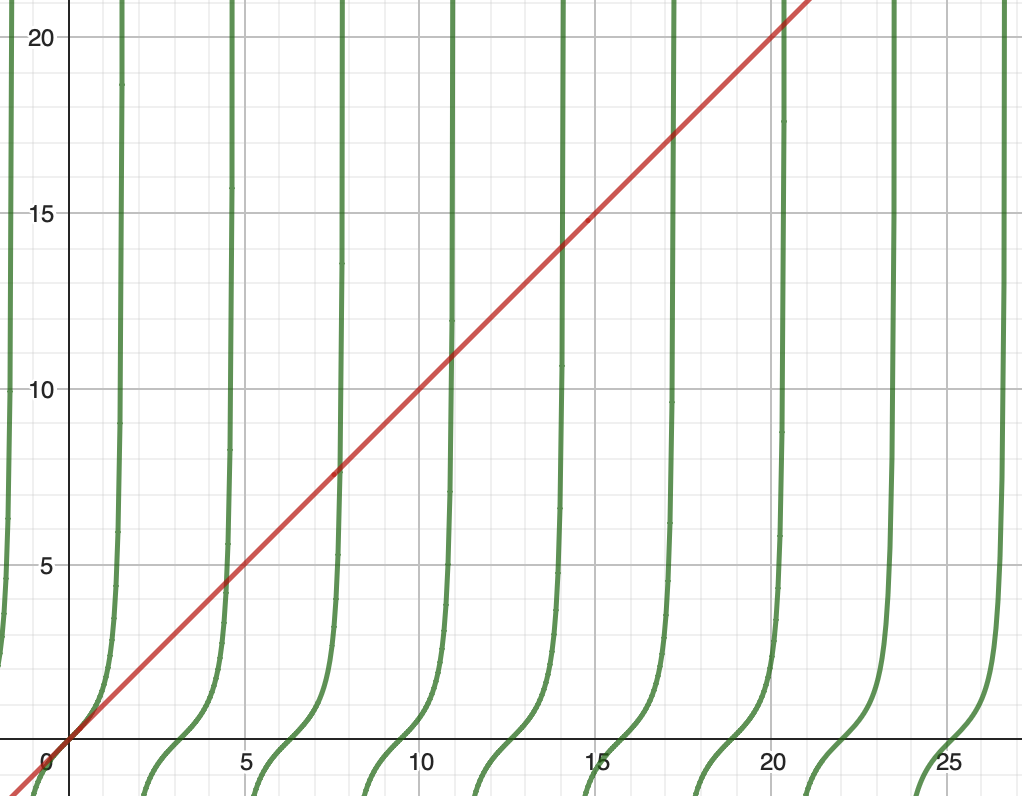
\includegraphics[height=8cm,width=18cm]{pdef}
If eigenvalue is negative $\ld =-\beta ^2$ where $\beta >0$, then $X$ must take the form 
 \begin{align*}
X=A \cosh (\beta x)+B \sinh (\beta x)
\end{align*}
The initial condition can now be rewritten as 
\begin{align*}
\begin{cases}
  \beta  B +A =0 \\
  A \cosh (\beta )+B \sinh (\beta )=0
\end{cases} \text{ or }\begin{bmatrix}
1& \beta  \\
\cosh (\beta ) & \sinh (\beta )
\end{bmatrix}\begin{bmatrix}
A\\
B
\end{bmatrix}=0
\end{align*}
This implies 
\begin{align*}
\beta = \tanh (\beta )
\end{align*}
This equation have no positive solution $\beta $, so there are no negative eigenvalues. 
\end{proof}
\begin{question}{}{}
Let $a_0<0,a_l>-a_0\text{ and }a_0+a_l<-a_0a_ll$. Solve the wave equations on finite interval with robin conditions 
\begin{align*}
\begin{cases}
  u_{tt}=c^2u_{xx}\text{ for }0<x<l\text{ \textbf{(Homogeneous DE)} }\\
  (u_x-a_0u)(0,t)=0\text{ and }(u_x+a_lu)(l,t)=0\text{ \textbf{(Robin BC)} }
\end{cases}
\end{align*}
\end{question}
\begin{proof}
Again, setting $u=XT$, we have 
 \begin{align*}
\begin{cases}
  X''+ \ld X=0 \\
  X'(0)-a_0X(0)=0 \\
  X'(l)+a_lX(l)=0
\end{cases}\text{ and }T''+c^2 \ld  T=0
\end{align*}
Because $a_0+a_l<-a_0a_ll$, we know $0$ is not an eigenvalue. If $\ld =\beta ^2 >0$ is an eigenvalue where $\beta >0$, then $X$ must take the form  $A\cos (\beta x)+B \sin (\beta x)$. Plugging the initial condition, we see that 
\begin{align*}
\begin{bmatrix}
  -a_0 & \beta \\
  a_l \cos (\beta l) - \beta \sin (\beta l) & \beta  \cos (\beta l)+ a_l \sin (\beta l) 
\end{bmatrix}\begin{bmatrix}
A \\
B
\end{bmatrix}=0
\end{align*}
This implies that $\ld =\beta ^2$ is an eigenvalue if and only if 
\begin{align}
  (a_0+a_l)\beta  \cos (\beta l)+ (a_0a_l-\beta ^2)\sin (\beta l)=0
\end{align}
It is then clear that the sets of positive eigenvalues is exactly 
\begin{align*}
\bset{\ld =\beta ^2\inr^+:\beta \neq \frac{(n+ \frac{1}{2})\pi }{l}\text{ and }\tan (\beta l)= \frac{(a_0+a_l)\beta }{\beta ^2- a_0a_l} }
\end{align*}
If $\ld =-\beta ^2<0$ is an eigenvalue where $\beta >0$, then $X$ must take the form  $A\cosh (\beta x)+ B\sinh (\beta x)$. Plugging the initial condition, we see that 
\begin{align*}
  \begin{bmatrix}
    -a_0 & \beta \\
    a_l \cosh (\beta l) + \beta \sinh (\beta l) & \beta  \cosh (\beta l)+a_l \sinh (\beta l)
  \end{bmatrix}
\begin{bmatrix}
A \\
B
\end{bmatrix}=0 
\end{align*}
This implies that $\ld =-\beta ^2$ is an eigenvalue if and only if 
\begin{align*}
  (a_0+a_l)\beta \cosh (\beta l)+ (a_0a_l+\beta ^2)\sinh (\beta l)=0 
\end{align*}
It is then clear that the set of negative eigenvalues is exactly 
\begin{align*}
\bset{\ld =-\beta ^2\inr^-: \beta^2\neq -a_0a_l\text{ and }\tanh (\beta l)= \frac{-(a_0+a_l)\beta }{a_0a_l+\beta ^2}}
\end{align*}
We have conclude that there are countable amount of positive eigenvalues $(\ld_n)_{n=1}$ and one negative eigenvalue $\ld _0$. This give us 
\begin{align*}
u&=\Big(A_0\cosh (c\sqrt{-\ld_0}t)+B_0\sinh (c \sqrt{-\ld_0}t ) \Big)\Big( \sqrt{-\ld_0}  \cosh (\sqrt{-\ld_0}x )+ a_0 \sinh (\sqrt{-\ld }x )  \Big) \\
&+\sum_{n=1}^{\infty} \Big(A_n \cos (c\sqrt{\ld _n}t )+B_n \sin (c\sqrt{\ld _n} t) \Big) \Big( \sqrt{\ld _n}\cos (\sqrt{\ld _n}x )+ a_0 \sin (\sqrt{\ld _n}x )  \Big)
\end{align*}
\end{proof}
\begin{question}{}{}
\begin{enumerate}[label=(\alph*)]
  \item Prove that the total energy is conserved for the wave equation with Dirichlet BCs, where the energy is defined to be 
    \begin{align}
    \label{ee}
    E= \frac{1}{2}\int_0^l \Big(\frac{u_t^2}{c^2}+u_x^2\Big)dx
    \end{align} 
    \item Do the same for the Neumann BCs. 
    \item For the Robin BCs, show that 
      \begin{align*}
      E_R= \frac{1}{2}\int_0^l \Big(\frac{u_t^2}{c^2}+u_x^2\Big)dx + \frac{a_l}{2}(u(l,t))^2 + \frac{a_0}{2}(u(0,t))^2
      \end{align*}
      is conserved. 
\end{enumerate}
\end{question}
\begin{proof}
If energy $E(t)$ is defined as in \myref{Equation}{ee}, then we have 
\begin{align*}
E'(t)&= \int_0^l \Big( \frac{u_tu_{tt}}{c^2}+u_xu_{xt} \Big)dx \\
&=\int_0^l (u_tu_{xx}+u_xu_{xt})dx \\
&=\int_0^l (u_tu_x)_xdx\\
&= u_tu_x(l,t)-u_tu_x(0,t)
\end{align*}
If we have the Dirichlet BCs, we see that $u_t(l,t)=u_t(0,t)=0$ by direct differentiation. If we have the Neumann BCs, we see that $u_x(l,t)=u_x(0,t)=0$. We now compute 
\begin{align*}
E_R'(t)&= u_tu_x(l,t)-u_tu_x(0,t)+ a_luu_t(l,t)+ a_0uu_t(0,t) \\
&=(u_x+a_lu)u_t(l,t)+ ( -u_x+  a_0u)u_t(0,t)
\end{align*}
which have $0$ coefficients  $(u_x+a_lu)(l,t)$ and $(-u_x+a_0u)(0,t)$ by Robin conditions. 
\end{proof}
\begin{question}{}{}
Consider a string  that is fixed at the en $x=0$ and is free at the end  $x=l$ except that a load of given mass is attached to the right end. 
 \begin{enumerate}[label=(\alph*)]
  \item Show that is satisfies the problem 
    \begin{align*}
    \begin{cases}
      u_{tt}=c^2u_{xx}\text{ for }0<x<l\text{ \textbf{(Homogeneous DE)} }  \\
      u(0,t)=0, u_{tt}(l,t)=-ku_x(l,t)\text{ \textbf{(BCs)} }
    \end{cases}
    \end{align*} 
    \item What is the eigenvalue problem in this case? 
    \item Find the equation for the positive eigenvalues and find the eigenfunctions. 
\end{enumerate}
\end{question}
\begin{proof}
The eigenvalue problem in this case is 
\begin{align*}
\begin{cases}
  X''+ \ld  X= 0\\
  X(0)=0\\
  c^2 X''(l)+ kX'(l)=0 
\end{cases}
\end{align*}
If $\ld =\beta ^2$ where $\beta >0$ is an eigenvalue, then $X$ must take the form  $A\cos (\beta x)+B \sin (\beta x)$, and boundary condition implies 
\begin{align*}
\begin{bmatrix}
  1 & 0 \\
  -c^2 \beta ^2 \cos (\beta l) - k \beta  \sin (\beta l) & -c^2 \beta ^2 \sin (\beta l)+ k \beta \cos (\beta l)
\end{bmatrix} \begin{bmatrix}
A \\
B
\end{bmatrix}= 0
\end{align*}
This implies the eigenspace is spanned by $\sin (\beta x)$ and the equation is 
\begin{align*}
k \beta  \cos (\beta l)= c^2 \beta ^2 \sin (\beta l)
\end{align*}
\end{proof}
\begin{question}{}{}
Solve the eigenvalue problem $x^2u''+3xu'+\ld u=0$ for $1<x<e$ with  $u(1)=u(e)=0$. Assume $\ld >1$. 
\end{question}
\begin{proof}
We first find the solution space of the differential equation. Let $u$ take the form $u=x^r$. Compute 
\begin{align*}
0&= x^r \big[r(r-1)+ 3r + \ld \big]   \\
&= x^r\big[ (r+1)^2 + \ld -1 \big]
\end{align*}
This implies 
\begin{align*}
r=-1 + \pm i \sqrt{\ld -1} 
\end{align*}
and implies that the solution space is spanned by 
\begin{align*}
\frac{\cos (\sqrt{\ld -1} \ln (x) )}{x}\text{ and }\frac{\sin (\sqrt{\ld -1}\ln (x) )}{x}
\end{align*}
Let 
\begin{align*}
u=A \frac{\cos (\sqrt{\ld -1} \ln (x))}{x}+ B \frac{\sin (\sqrt{\ld -1} \ln (x))}{x}
\end{align*}
Boundary condition then implies 
\begin{align*}
\begin{bmatrix}
  1 & 0 \\
  \frac{\cos (\sqrt{\ld -1} )}{e} & \frac{\sin (\sqrt{\ld -1} )}{e}
\end{bmatrix} \begin{bmatrix}
A\\
B
\end{bmatrix}=0
\end{align*}
The eigenvalues greater than $1$ are then $\ld =n^2\pi ^2+1$ with eigenfunction $\frac{\sin (\sqrt{\ld-1} \ln (x) )}{x}$ 
\end{proof}

\section{5.1 The coefficient}
\begin{mdframed}
When $n\neq m \inz^*$, we may compute 
\begin{align*}
\int_0^{\pi} \sin (nx) \sin (mx)dx &= \frac{1}{-4}\int_0^\pi (e^{i nx}- e^{-inx})(e^{imx}-e^{-imx})dx \\
&= \frac{1}{-4}\int_0^{\pi} \big(e^{i(n+m)x} -e^{i (m-n)x}-e^{i(n-m)x}+e^{i (-n-m)x} \big)dx\\
&=\frac{1}{-4}\Big[ \frac{e^{i(n+m)x}- e^{-i(n+m)x}}{i(n+m)}+ \frac{e^{i(m-n)x}-e^{i(n-m)x}}{i(n-m)} \Big] \Big|_{x=0}^{\pi}=0
\end{align*}
If $n=m$, we may compute 
 \begin{align*}
\int_0^{\pi} \sin(nx)\sin (nx)dx &= \frac{1}{-4}\int_0^{\pi} \big( e^{2inx}+e^{-2inx}-2 \big)dx= \frac{\pi }{2}
\end{align*}
We then can conclude 
\begin{align*}
\int_0^l \sin (\frac{n \pi x}{l}) \sin (\frac{m \pi x}{l})dx=\frac{l}{\pi}\int_0^\pi \sin (n u)\sin (m u)du= \begin{cases}
  0& \text{ if $n\neq m$ }\\
  \frac{l}{2}& \text{ if $n=m$ }
\end{cases}
\end{align*}
When $n\neq m \inz^*$, we may compute 
\begin{align*}
\int_0^{\pi} \cos (nx) \cos (mx)dx &= \frac{1}{4}\int_0^\pi (e^{i nx}+ e^{-inx})(e^{imx}+e^{-imx})dx \\
&= \frac{1}{4}\int_0^{\pi} \big(e^{i(n+m)x} +e^{i (m-n)x}+e^{i(n-m)x}+e^{-i(n+m)x} \big)dx\\
&=\frac{1}{4}\Big[ \frac{e^{i(n+m)x}- e^{-i(n+m)x}}{i(n+m)}+ \frac{e^{i(n-m)x}-e^{i(m-n)x}}{i(n-m)} \Big] \Big|_{x=0}^{\pi}=0
\end{align*}
If $n=m$, we may compute 
 \begin{align*}
\int_0^{\pi} \cos(nx)\cos (nx)dx &= \frac{1}{4}\int_0^{\pi} \big( e^{2inx}+e^{-2inx}+2 \big)dx= \frac{\pi }{2}
\end{align*}
We then can conclude 
\begin{align*}
\int_0^l \cos (\frac{n \pi x}{l}) \cos (\frac{m \pi x}{l})dx=\frac{l}{\pi}\int_0^\pi \cos (n u)\cos (m u)du= \begin{cases}
  0& \text{ if $n\neq m$ }\\
  \frac{l}{2}& \text{ if $n=m$ }
\end{cases}
\end{align*}
This also give us 
\begin{align*}
&\int_{-l}^{l} \sin^2 (\frac{n \pi  x}{l})dx=\int_{-l}^{l}\cos^2 ( \frac{n\pi  x}{l})dx=l\\
&\int_{-l}^{l} \sin (\frac{n \pi  x}{l})\sin (\frac{m \pi  x}{l})dx=\int_{-l}^l \cos( \frac{n \pi  x}{l})\cos (\frac{n \pi  x}{l})dx=0
\end{align*}
\begin{align*}
  \int_{-l}^{l} \cos^2 (\frac{n \pi  x}{l})dx&= \int_{-l}^{l}\sin ^2 (\frac{n \pi  x}{l})dx= l\\
 \int_0^l \cos^2 (\frac{n \pi  x}{l})dx&=\int_0^l \sin^2 (\frac{n \pi  x}{l})dx=\frac{l}{2} 
\end{align*}

\end{mdframed}
\begin{question}{}{}
In the expansion $1=\sum_{n\operatorname{ odd}}(\frac{4}{n\pi})\sin (nx)$, valid for $x\in (0,\pi)$, put $x= \frac{\pi}{4}$ to calculate the sum 
\begin{align*}
  &(1-\frac{1}{5}+\frac{1}{9}-\frac{1}{13}+\cdots) + (\frac{1}{3}-\frac{1}{7}+\frac{1}{11}-\frac{1}{15}+\cdots) \\
  &= 1+ \frac{1}{3} - \frac{1}{5} - \frac{1}{7} + \frac{1}{9} + \cdots 
\end{align*}
\end{question}
\begin{proof}
What? 
\end{proof}
\begin{question}{}{}
Let $\phi (x)\equiv x^2$ for $0\leq x\leq 1=l$. 
\begin{enumerate}[label=(\alph*)]
  \item Calculate its Fourier sine series. 
  \item Calculate its Fourier cosine series. 
\end{enumerate}
\end{question}
\begin{proof}
Write 
\begin{align*}
  \phi (x)= \sum_{n=0}^{\infty}B_n \sin (n\pi x)
\end{align*}
and 
\begin{align*}
  \int_0^1 \phi (x) \sin (n \pi  x)dx= B_n\int_0^1 \sin^2(n \pi  x)dx=\frac{B_n}{2}
\end{align*}
This give us  
\begin{align*}
\frac{B_n}{2}&= \int_0^{1} x^2 \sin (n \pi x)dx  \\
&= \frac{(-1)^n}{- n \pi}+  \frac{2}{n \pi}\int_0^1 x \cos (n\pi x)dx\\
&= \frac{(-1)^n}{- n \pi} - \frac{2}{n^2 \pi^2 }\int_0^1 \sin(n\pi x)dx \\
&=\frac{(-1)^n}{-n \pi }+ \frac{2(-1)^n-2}{n^3\pi ^3}\\
&= \frac{n^2\pi ^2(-1)^{n+1}+ 2(-1)^n -2}{n^3\pi ^3}
\end{align*}
and 
\begin{align*}
x^2=\sum_{n=0}^{\infty} \frac{2\big(-2+(-1)^n(2-n^2\pi ^2) \big)}{n^3\pi ^3} \sin (n\pi  x)
\end{align*}
Write 
\begin{align*}
\phi (x)=\sum_{n=0}^{\infty}A_n \cos (n \pi  x) 
\end{align*}
and 
\begin{align*}
\int_0^1 \phi (x)\cos (n \pi  x)dx=A_n\int_0^1 \cos^2(n \pi  x)dx= \frac{A_n}{2}
\end{align*}
This give us 
\begin{align*}
\frac{A_n}{2}&= \int_0^1 x^2 \cos (n \pi  x)dx\\
&= \frac{-2}{n \pi }\int_0^1x \sin (n \pi  x)dx\\
&=\frac{-2}{n\pi }\Big( \frac{-(-1)^n}{n \pi }+ \frac{1}{n \pi }\int_0^1 \cos (n \pi x)dx \Big)= \frac{2(-1)^n}{n^2 \pi ^2}
\end{align*}
and $A_0=\frac{2}{3}$. This give us 
\begin{align*}
\phi (x)= \frac{2}{3}+\sum_{n=1}^{\infty} \frac{4(-1)^n}{n^2 \pi ^2}\cos (n \pi  x)
\end{align*}
\end{proof}
\begin{question}{}{}
Find the Fourier cosine series of the function $\abso{\sin x}$ in the interval $(-\pi  ,\pi )$. Use it to find the sums 
\begin{align*}
\sum_{n=1}^{\infty} \frac{1}{4n^2-1}\text{ and }\sum_{n=1}^{\infty} \frac{(-1)^n}{4n^2-1}
\end{align*}
\end{question}
\begin{proof}
Write 
\begin{align*}
\abso{\sin x}= \sum_{n=0}^{\infty}A_n \cos (nx)
\end{align*}
Compute
\begin{align*}
  A_0&=\frac{1}{2\pi }\int_{-\pi }^{\pi } A_0 \cos (0x)dx\\
  &=\frac{1}{2\pi }\sum_{n=0}^{\infty} \int_{-\pi }^{\pi }A_n \cos (nx)dx \\
  &=\frac{1}{2\pi } \int_{-\pi }^{\pi } \abso{\sin x}dx= \frac{2}{\pi }
\end{align*}
Compute for all $n\inn \setminus \set{1}$
\begin{align*}
A_n&= \frac{1}{\pi }\int_{-\pi }^{\pi }A_n \cos^2 (nx)dx \\
&=\frac{1}{\pi }\sum_{m=0}^{\infty}\int_{-\pi }^{\pi }A_m \cos (mx)\cos (nx)dx \\
&=\frac{1}{\pi }\int_{-\pi }^{\pi }\Big(\sum_{m=0}^{\infty} A_m \cos (mx)\Big)\cos (nx)dx \\
&=\frac{1}{\pi }\int_{-\pi }^{\pi }\abso{\sin x}\cos (nx)dx\\
&=\frac{-1}{\pi }\Big(\frac{(-1)^{n+1}-1}{n+1}- \frac{(-1)^{n-1}-1}{n-1} \Big)= \frac{2((-1)^{n+1}-1)}{\pi  (n^2-1)}
\end{align*}
Compute 
\begin{align*}
A_1&= \frac{1}{\pi } \int_{-\pi }^{\pi }A_1\cos ^2(x)dx \\
&=\frac{1}{\pi }\sum_{m=0}^{\infty}\int_{-\pi }^{\pi }A_m \cos (mx)\cos (x)dx \\
&=\frac{1}{\pi }\int_{-\pi }^{\pi }\Big( \sum_{m=0}^{\infty}A_m \cos (mx) \Big) \cos (x)dx \\
&=\frac{1}{\pi }\int_{-\pi }^{\pi } \abso{\sin (x)}\cos (x)dx =0 
\end{align*}
We have shown 
\begin{align*}
\abso{\sin (x)}&= \frac{2}{\pi }+ \sum_{n=2}^{\infty} \frac{2((-1)^{n+1}-1)}{\pi  (n^2-1)}\cos (nx) \\
&=\frac{2}{\pi }+ \sum_{n\text{ even }}\frac{2((-1)^{n+1}-1)}{\pi  (n^2-1)}\cos (nx)\\
&=\frac{2}{\pi }+ \sum_{k\inn} \frac{-4}{\pi  (4k^2-1)}\cos (2kx)
\end{align*}
Plugging $x=0$, we see 
 \begin{align*}
\sum_{k\inn} \frac{1}{4k^2-1}= \frac{1}{2}
\end{align*}
Plugging $x=\frac{\pi }{2}$, we see 
\begin{align*}
1&= \frac{2}{\pi }+ \sum_{k\inn} \frac{-4}{\pi  (4k^2-1)}\cos (k\pi ) \\
&= \frac{2}{\pi }+ \sum_{k\inn} \frac{-4}{\pi  (4k^2-1)}(-1)^k \\
\end{align*}
That is 
\begin{align*}
  \frac{\pi  -2}{-4}= \sum_{k\inn} \frac{(-1)^k}{4k^2-1}
\end{align*}
\end{proof}
\begin{question}{}{}
\begin{enumerate}[label=(\alph*)]
  \item Find the sine series of $x^3$ on  $(0,l)$.
  \item Find the cosine series of $x^4$ on $(0,l)$.
\end{enumerate}
\end{question}
\begin{proof}
Write 
\begin{align*}
x^3 = \sum_{n=1}^{\infty}A_n \sin (\frac{n \pi  x}{l})
\end{align*}
Then for all $n\inn$, we have 
\begin{align*}
\int_0^l x^3 \sin (\frac{n \pi  x}{l})dx&= \int_0^l \sum_{m=1}^{\infty} A_m \sin (\frac{m \pi  x}{l})\sin (\frac{n \pi  x}{l})dx \\
&= \frac{A_n l}{2}
\end{align*}
Compute 
\begin{align*}
\int_0^l x^3 \sin (\frac{ n \pi  x}{l})dx= \frac{- l^4 (-1)^n}{ n \pi  } + \frac{6l^4 (-1)^n}{n^3 \pi ^3} 
\end{align*}
This give us 
\begin{align*}
A_n= (-1)^nl^3 \Big(\frac{-2}{n \pi }+ \frac{12}{n^3 \pi ^3}\Big)
\end{align*}
That is 
\begin{align*}
x^3= \sum_{n=1}^{\infty} (-1)^n l^3 \Big(\frac{-2}{n \pi  }+ \frac{12}{n^3 \pi ^3} \Big) \sin (\frac{n \pi x }{l})
\end{align*}
Integrating both side, we have 
\begin{align*}
\frac{x^4}{4}+C&= \sum_{n=1}^{\infty} (-1)^n l^3 \Big( \frac{-2}{n\pi }+ \frac{12}{n^3 \pi ^3} \Big) \int  \sin (\frac{n \pi  x}{l})dx \\
&=\sum_{n=1}^{\infty} (-1)^n l^3 \Big( \frac{-2}{n\pi }+ \frac{12}{n^3 \pi ^3} \Big) \Big(\frac{-l\cos (\frac{n \pi  x}{l})}{n \pi }+C_n  \Big)
\end{align*}
Simplifying the result 
\begin{align*}
x^4=C_0 + \sum_{n=1}^{\infty} (-1)^n l^4 \Big( \frac{8}{n^2 \pi ^2}+ \frac{-48}{n^4 \pi ^4} \Big)\cos (\frac{n \pi  x}{l})
\end{align*}
Note that 
\begin{align*}
\frac{l^5}{5}=\int_0^l x^4dx=\int_0^l C_0dx= lC_0
\end{align*}
This give us 
\begin{align*}
x^4= \frac{l^4}{5}+ \sum_{n=1}^{\infty} (-1)^n l^4 \Big( \frac{8}{n^2\pi ^2}+ \frac{-48}{n^4\pi  ^4} \Big) \cos (\frac{n \pi  x}{l})
\end{align*}
\end{proof}
\begin{question}{}{}
Put $x=0$ in the last question to compute 
 \begin{align*}
\sum_1 \frac{(-1)^n}{n^4}
\end{align*}
\end{question}
\begin{proof}
Putting $x=0$ and divided both side with  $l^4$ in last question, we have 
\begin{align*}
0= \frac{1}{5}+ \sum_{n=1}^{\infty} (-1)^n \Big(\frac{8}{n^2 \pi ^2} + \frac{-48}{n^4 \pi ^4}\Big)
\end{align*}
This give us 
\begin{align*}
\sum_{n=1}^{\infty} \frac{(-1)^n}{n^4}&= \frac{\pi  ^4}{-48} \Big( \frac{-1}{5}-\sum_{n=1}^{\infty} \frac{8(-1)^n}{n^2 \pi ^2} \Big) \\
&=\frac{\pi ^4}{-48}\Big( \frac{-1}{5}- \frac{8}{\pi ^2} \sum_{n=1}^{\infty} \frac{(-1)^n}{n^2} \Big) \\
&=\frac{\pi ^4}{-48}\Big( \frac{-1}{5}+ \frac{2}{3} \Big)= \frac{7 \pi ^4}{-720}
\end{align*}
\end{proof}
\begin{question}{}{}
Solve 
\begin{align*}
\begin{cases}
  u_{tt}=c^2u_{xx}\text{ for }0<x<\pi \text{ \textbf{(Homogeneous DE)} }  \\
  u_x(0,t)= u_x(\pi ,t)=0\text{ \textbf{(Newman BC)} } \\
  u(x,0)=0,u_t(x,0)=\cos ^2(x)\text{ \textbf{(IC)} }
\end{cases}
\end{align*}
\end{question}
\begin{proof}
  We see that $u=XT$ satisfy the DE and BC as long as 
   \begin{align*}
  \begin{cases}
    X''+ \ld X=0  \\
    X'(0)=X'(\pi )=0
  \end{cases} \text{ and } T''+c^2 \ld  T=0
  \end{align*}
for some constant $\ld \inc$. It is clear that for $X$, $0$ is an eigenvalue with constant eigenfunction, and the rest of the eigenvalues are $\ld_n=n^2$ with eigenfunction $\cos (nx)$. This give us 
\begin{align*}
u=A_0 (B_0+C_0t)+\sum_{n=1}^{\infty} A_n\cos (nx) \big(B_n \cos (cnt)+C_n \sin (cnt)  \big)
\end{align*}
A change of notation give us  
\begin{align*}
u=A_0+B_0t + \sum_{n=1}^{\infty} A_n \cos (nx)\cos (cnt) + B_n \cos (nx)\sin (cnt)
\end{align*}
Plug in the initial condition $u(x,0)=0$, we see 
\begin{align*}
0=A_0+ \sum_{n=1}^{\infty}A_n \cos (nx)
\end{align*}
Because constants have Fourier coefficient all $0$ except the first term, we may now deduce $A_0=A_n=0$. We now may write 
 \begin{align*}
u=B_0t+\sum_{n=1}^{\infty} B_n \cos (nx)\sin (cnt)
\end{align*}
Compute 
\begin{align*}
u_t=B_0 + \sum_{n=1}^{\infty}B_ncn \cos (nx)\cos (cnt)
\end{align*}
Plug in the initial condition $\cos^2(x)=u_t(x,0)$, we see 
\begin{align*}
\cos ^2(x)=B_0 + \sum_{n=1}^{\infty}B_ncn\cos (nx)
\end{align*}
We now compute the Fourier cosine series of $\cos ^2(x)$ on $(0,\pi )$. 
\begin{align*}
\cos^2(x)=  \frac{1+\cos (2x)}{2}
\end{align*}
This give us $B_0= \frac{1}{2}$ and 
\begin{align*}
B_n\triangleq \begin{cases}
  \frac{1}{4c}& \text{ if $n=2$ }\\
  0& \text{ if $n\neq 2$ }
\end{cases}
\end{align*}
In summary 
\begin{align*}
u=\frac{t}{2}+ \frac{\cos (2x)\sin (2ct) }{4c}
\end{align*}
\end{proof}
\chapter{PDE 4}
\section{Cheat Sheet}
\begin{mdframed}
Consider the \textbf{Dirichlet} eigenproblem 
\begin{align*}
\begin{cases}
  X''+ \ld X=0 \\
  X(0)=X(l)=0
\end{cases}
\end{align*}
It is clear that $0$ is NOT an eigenvalue. Suppose  $\ld =\beta ^2\inc$ is an eigenvalue. We see that $X$ must take the form
\begin{align*}
X= A \cos (\beta x)+ B \sin (\beta x)
\end{align*}
The initial condition implies 
\begin{align*}
\begin{bmatrix}
  1 & 0  \\
  \cos (\beta l) & \sin (\beta l)
\end{bmatrix} \begin{bmatrix}
A\\
B
\end{bmatrix}=0 
\end{align*}
This implies that 
\begin{align*}
\beta = \frac{n \pi  }{l}\text{ and } X= \sin ( \frac{n \pi  x}{l})\text{ for }n\geq 1
\end{align*}
\end{mdframed}
\begin{mdframed}
  Consider the \textbf{Neumann} eigenproblem 
\begin{align*}
\begin{cases}
  X'' + \ld X=0 \\
  X'(0)=X'(l)=0
\end{cases}
\end{align*}
It is clear that $0$ is an eigenvalue with eigenspace spanned by constant function. Suppose $\ld =\beta ^2\inc$ is an eigenvalue. We see that $X$ must take the form 
 \begin{align*}
X= A\cos (\beta x) + B\sin (\beta x)
\end{align*}
The initial condition then implies 
\begin{align*}
\begin{bmatrix}
  0 & \beta \\
  -\beta  \sin (\beta l) & \beta  \cos (\beta l)
\end{bmatrix}\begin{bmatrix}
A\\
B
\end{bmatrix}=0 
\end{align*}
This implies that 
\begin{align*}
\beta = \frac{n \pi  }{l} \text{ and }X= \cos (\frac{n \pi  x}{l})\text{ for }n\geq 1
\end{align*}
\end{mdframed}
\begin{mdframed}
Consider the \textbf{mixed} eigenproblem 
\begin{align*}
\begin{cases}
  X''+ \ld  X=0 \\
  X(0)=X'(l)=0
\end{cases}
\end{align*}
It is clear that $0$ is Not an eigenvalue. Suppose $\ld = \beta ^2\inc$ is an eigenvalue. We see that $X$ must take the form 
 \begin{align*}
X=A \cos (\beta x)+ B \sin (\beta x)
\end{align*}
The initial condition implies 
\begin{align*}
\begin{bmatrix}
  1 & 0 \\
  -\beta  \sin (\beta l) & \beta \cos (\beta l) 
\end{bmatrix} \begin{bmatrix}
A \\
B
\end{bmatrix}=0 
\end{align*}
This implies
\begin{align*}
\beta = \frac{(n+ \frac{1}{2})\pi }{l}\text{ and }X_n= \sin (\frac{(n+ \frac{1}{2})\pi  x}{l})\text{ for }n\geq 1
\end{align*}
\end{mdframed}
\begin{mdframed}
The \textbf{Fourier sine series of $\phi$ on $(0,l)$} is 
  \begin{align*}
  \phi (x)=\sum_{n=0}^{\infty} A_n \sin (\frac{n \pi  x}{l})
  \end{align*}
The \textbf{Fourier cosine series of $\phi$ on $(0,l)$} is 
  \begin{align*}
  \phi (x)=\sum_{n=0}^{\infty} A_n \cos (\frac{n \pi  x}{l})
  \end{align*}
The \textbf{Fourier full series of $\phi$ on $(-l,l)$} us 
\begin{align*}
\phi (x)= \sum_{n=0}^{\infty} A_n \cos (\frac{n \pi  x}{l})+ B_n \sin ( \frac{n \pi  x}{l})
\end{align*}
The \textbf{Fourier complex series of $\phi$ on $(-l,l)$ is}
\begin{align*}
\phi (x)=\sum_{n=-\infty}^{\infty}  c_n e^{\frac{- i n \pi  x}{l}}
\end{align*}
\end{mdframed}
\begin{mdframed}
Let $n,m\neq 0$. To compute the sine series, we have 
\begin{align*}
\int_0^l \sin (\frac{n \pi  x}{l})\sin (\frac{m \pi  x}{l})dx=\begin{cases}
  \frac{l}{2}& \text{ if $n= m$ } \\
  0& \text{ if $n\neq m$ }
\end{cases}
\end{align*}
Let $n,m\neq 0$. To compute the cosine series, we have 
\begin{align*}
\int_0^l \cos (\frac{n \pi  x}{l})\cos (\frac{m \pi  x}{l})dx= \begin{cases}
  \frac{l}{2}& \text{ if $n= m$ }\\
  0& \text{ if $n \neq m$ }
\end{cases}
\end{align*}
Let $n,m\neq 0$. To compute the full series, we have 
\begin{align*}
\int_{-l}^{l} \sin (\frac{n \pi  x}{l})\sin (\frac{m \pi  x}{l})dx= \begin{cases}
  l& \text{ if $n=m$ }\\
  0& \text{ if $n\neq  m$ }
\end{cases}
\end{align*}
and 
\begin{align*}
\int_{-l}^{l} \cos (\frac{n \pi  x}{l}) \cos ( \frac{m \pi  x}{l})dx=\begin{cases}
  l& \text{ if $n=m$ }\\
  0& \text{ if $n\neq m$ }
\end{cases}
\end{align*}
Let $n,m \inz$. To compute the complex series, we have 
\begin{align*}
\int_{-l}^{l} e^{\frac{i (n-m)\pi  x}{l}}dx= \begin{cases}
  2l & \text{ if $n=m$ }\\
  0& \text{ if $n\neq m$ }
\end{cases}
\end{align*}
Let $n,m\geq  0$. To compute the weird series, we have 
\begin{align*}
  \int_0^l \sin (\frac{(n+ \frac{1}{2})\pi  x}{l}) \sin (\frac{(m+ \frac{1}{2})\pi  x}{l})dx = \begin{cases}
    \frac{l}{2}& \text{ if $n=m$ }\\
    0& \text{ if $n\neq m$ }
  \end{cases}
\end{align*}
and 
\begin{align*}
  \int_0^l \cos (\frac{(n+ \frac{1}{2})\pi  x}{l}) \cos (\frac{(m+ \frac{1}{2})\pi  x}{l})dx = \begin{cases}
    \frac{l}{2}& \text{ if $n=m$ }\\
    0& \text{ if $n\neq m$ }
  \end{cases}
\end{align*}
\end{mdframed}
\section{5.2 Even, Odd, Periodic and Complex Functions}
\begin{question}{}{}
Show that $\cos x+ \cos (\alpha x)$ is periodic if $\alpha $ is a rational number. What is its period? Show that $\cos x+ \cos (\sqrt{2}x)$ is not periodic. 
\end{question}
\begin{proof}
If $\alpha \inq$, we may write 
\begin{align*}
\alpha = \frac{q}{p}\text{ where }p \inn
\end{align*}
we then see $\cos x+ \cos (\alpha x)$ has period $2p \pi $. \As{$\cos x+ \cos (\sqrt{2}x )$ have period $r$}. Then 
\begin{align*}
2= \cos (r)+ \cos (\sqrt{2}r )
\end{align*}
which is easily seen impossible by noting for this to be true we must have $r= 2n \pi $. 
\end{proof}
\begin{question}{}{}
Prove 
\begin{enumerate}[label=(\alph*)]
  \item If $\phi$ is an odd function, its full Fourier series on $(-l,l)$ has only sine terms. 
  \item Also, if $\phi$ is an even function, its full Fourier series on $(-l,l)$ has only cosine terms. (Hint: Don't use the series directly. Use the formulas for the coefficients to show that every second coefficient vanishes.)
\end{enumerate}
\end{question}
\begin{proof}
Write 
\begin{align*}
\phi = \sum_{n=0}^{\infty} A_n \cos (\frac{n \pi  x}{l})+ B_n \sin ( \frac{n \pi  x}{l})
\end{align*}
Compute 
\begin{align*}
A_nl=\int_{-l}^{l} \phi (x) \cos (\frac{ n \pi  x}{l})dx=0\text{ for all }n\geq 1
\end{align*}
if $\phi$ is odd. Compute 
\begin{align*}
B_nl = \int_{-l}^{l} \phi (x)\sin ( \frac{n \pi  x}{l})dx=0\text{ for all }n\geq 1
\end{align*}
if $\phi$ is even. 
\end{proof}
\begin{question}{}{}
Let $\phi(x)$ be a function of period $\pi $. If $\phi (x)=\sum_{n=1}^{\infty}a_n \sin (nx)$ for all $x$, find the odd coefficients. 
\end{question}
\begin{proof}
Because $\phi$ has period $\pi $, we have 
\begin{align*}
\sum_{n=1}^{\infty} a_n \sin (nx)= \phi (x)= \phi (x+ \pi )&= \sum_{n=1}^{\infty}a_n \sin (nx+ n \pi )\\
&=\sum_{n=1}^{\infty}(-1)^na_n \sin (nx)
\end{align*}
For this to be true, we must have $a_{\operatorname{odd}}=0$. 
\end{proof}
\begin{question}{}{}
Find the full Fourier series of $e^x$ on  $(-l,l)$ in its real and complex forms. (Hint: It is convenient to find the complex form first)
\end{question}
\begin{proof}
Write 
\begin{align*}
e^x= \sum_{n=- \infty}^{\infty} c_n e^{ \frac{i n \pi x }{l}}
\end{align*}
Compute 
\begin{align*}
c_n&= \frac{1}{2l}\int_{-l}^{l}e^x e^{\frac{- i n \pi  x}{l}}dx \\
&=\frac{1}{2l}\int_{-l}^{l}e^{ \frac{(l-i n\pi )x}{l}}dx\\
&=\frac{1}{2l} \cdot \frac{le^{\frac{(l-i n \pi )x}{l}}}{l-i n \pi  }\Big|_{x=-l}^{l} \\
&= \frac{l(e^{l- i n \pi }- e^{-(l- i n \pi )})}{2l (l- i n \pi )}\\
&= \frac{(-1)^n (e^l - e^{-l})}{2(l - i n \pi )}= \frac{(-1)^n}{(l- i n \pi )}\sinh (l)
\end{align*}
We now have 
\begin{align*}
e^x&= \sum_{n=-\infty}^{\infty} \frac{(-1)^n}{(l- i n \pi )}\sinh (l) e^{\frac{i n \pi x}{l}} \\
&= \frac{\sinh (l)}{l}+ \sum_{n=1}^{\infty} \Big[\frac{(-1)^n \sinh (l) }{(l- i n \pi )}e^{\frac{i n \pi  x}{l}}+ \frac{(-1)^n \sinh (l)}{(l+ i n \pi )}e^{\frac{- i n \pi x}{l}}  \Big] \\
&=\frac{\sinh (l)}{l}+ \sum_{n=1}^{\infty} (-1)^n\sinh (l) \Big[ \frac{\cos (\frac{n \pi  x}{l})+ i \sin (\frac{n \pi  x}{l})}{l- i n \pi }+ \frac{\cos (\frac{n \pi  x}{l})- i \sin (\frac{n \pi  x}{l})}{l+ i n \pi } \Big]\\
&= \frac{\sinh (l)}{l}\\
&+ \sum_{n=1}^{\infty} (-1)^n \sinh (l) \cdot \frac{(l+ i n \pi )\big(\cos (\frac{n \pi  x}{l})+i \sin (\frac{n \pi  x}{l})  \big)+(l- i n \pi )\big( \cos (\frac{n \pi  x}{l})- i \sin (\frac{n \pi  x}{l}) \big)}{l^2 + n^2 \pi ^2} \\
&=\frac{\sinh (l)}{l}+ \sum_{n=1}^{\infty} \frac{(-1)^n \sinh (l)\big[ 2l \cos (\frac{n \pi  x}{l})-2n \pi  \sin (\frac{n \pi  x}{l}) \big]}{l^2+n^2\pi  ^2} \\
&= \sum_{n=0}^{\infty} \frac{2(-1)^n \sinh (l)}{l^2 + n^2 \pi ^2}\Big[l\cos (\frac{n \pi  x}{l})- n \pi  \sin (\frac{n \pi  x}{l}) \Big]
\end{align*}

\end{proof}
\begin{question}{}{}
Repeat the last exercise for $\cosh (x)$
\end{question}
\begin{proof}
Recall from last exercise that 
\begin{align*}
e^x= \sum_{n=- \infty}^{\infty} \frac{(-1)^n \sinh (l)}{l-i n \pi }  e^{ \frac{i n \pi  x}{l}}
\end{align*}
This give us 
\begin{align*}
\cosh (x) =\frac{1}{2}(e^{x}-e^{-x})= \frac{1}{2}\Big( \sum_{n=-\infty}^{\infty} \frac{(-1)^n \sinh (l)}{l- i n \pi }e^{ \frac{i n \pi  x}{l}}+ \sum_{n=-\infty}^{\infty} \frac{(-1)^n \sinh (l)}{l- i n \pi }e^{\frac{-i n \pi  x}{l}} \Big)
\end{align*}
\end{proof}
\begin{question}{}{}
Repeat the last exercise for $\sin x$. Assume that $l$ is not an integer multiple of  $\pi $. (Hint: First find the series for $e^{ ix}$)
\end{question}
\begin{proof}

\end{proof}
\section{5.3 Orthogonality and General Fourier Series} 
\begin{mdframed}
In this section, we are concerned with the eigenproblem 
\begin{align*}
X''+\ld  X= 0\text{ on }(a,b)
\end{align*}
with a pair of boundary conditions 
\begin{align*}
\begin{cases}
  \alpha_1 X(a)+ \beta _1 X(b)+ \gamma_1 X'(a)+ \delta_1 X'(b)=0 \\
  \alpha_2 X(a) + \beta _2 X(b)+ \gamma _2 X'(a)+ \delta_2 X'(b)=0
\end{cases}
\end{align*}
where the coefficients $\alpha ,\beta ,\gamma\text{ and }\delta$ are all real. A pair of boundary condition is called \textbf{symmetric} if every pair of function $f,g:(a,b)\rightarrow \C$ that satisfies the boundary conditions also satisfies   
\begin{align*}
  f'(x)\overline{g(x)}-f(x)\overline{g'(x)} \Big|_{x=a}^b =0
\end{align*}
Immediately, we see that if the boundary condition is symmetric, two eigenfunction $X_1,X_2$ with distinct eigenvalues are either orthogonal or have conjugate eigenvalues since 
 \begin{align*}
   (\ld _1- \overline{\ld _2})\int_a^b X_1  \overline{X_2} dx&= \int_a^b (-X_1''\overline{ X_2}+ X_1\overline{X_2''})dx \\
                                                                      &= (-X_1'\overline{X_2}+X_1\overline{X_2'})\Big|_{x=a}^b=0
\end{align*}
The second equality is often referred to as \textbf{Green's second identity}. 
\end{mdframed}
\begin{question}{}{}
Consider $u_{tt}=c^2 u_{xx}$ for $0<x<l$, with the boundary conditions  $u (0,t)=u_x(l,t)=0$, and the initial condition $u(x,0)=x,u_t(x,0)=0$. Find the solution explicitly in series form. 
\end{question}
\begin{proof}
The eigenproblems are 
\begin{align*}
\begin{cases}
  X''+ \ld  X=0 \\
  X(0)=X'(l)=0
\end{cases} \text{ and }\begin{cases}
  T''+ c^2 \ld T=0
\end{cases}
\end{align*}
Direct computation shows that $\ld \neq 0$. If $\ld=\beta ^2$, and $X= A \cos (\beta x)+B \sin (\beta x)$, then BCs give 
\begin{align*}
\begin{bmatrix}
  1 & 0 \\
  -\beta  \sin (\beta l) & \beta \cos (\beta l) 
\end{bmatrix} \begin{bmatrix}
A \\
B
\end{bmatrix}=0 
\end{align*}
This implies
\begin{align*}
\beta = \frac{(n+ \frac{1}{2})\pi }{l}\text{ and }X_n= \sin (\frac{(n+ \frac{1}{2})\pi  x}{l})
\end{align*}
and $T_n= A_n\cos (c \beta t)+ B_n \sin (c \beta t)$. We now may write 
\begin{align*}
u= \sum_{n=0}^{\infty} \Big(A_n \cos (\frac{(n+\frac{1}{2})c \pi t  }{l}) + B_n \sin (\frac{(n+\frac{1}{2})c \pi  t}{l})  \Big) \sin ( \frac{(n+ \frac{1}{2})\pi  x}{l})
\end{align*}
Compute 
\begin{align*}
u_t= \sum_{n=0}^{\infty} \frac{(n+ \frac{1}{2})c \pi  }{l}  \Big(-A_n  \sin  (\frac{(n+\frac{1}{2})c \pi t  }{l}) + B_n \cos (\frac{(n+\frac{1}{2})c \pi  t}{l})  \Big) \sin ( \frac{(n+ \frac{1}{2})\pi  x}{l})
\end{align*}
Plugin the ICs, we now have 
\begin{align*}
x=\sum_{n=0}^{\infty} A_n \sin (\frac{(n+ \frac{1}{2})\pi  x}{l})
\end{align*}
and 
\begin{align*}
0=\sum_{n=0}^{\infty} \frac{(n+ \frac{1}{2})c \pi  }{l}  B_n   \sin ( \frac{(n+ \frac{1}{2})\pi  x}{l})
\end{align*}
Because 
\begin{align*}
\int_0^l \sin (\frac{(n+\frac{1}{2})\pi  x}{l}) \sin ( \frac{(m+\frac{1}{2})\pi  x}{l}) dx= \begin{cases}
  \frac{l}{2}& \text{ if $n=m$ }\\
  0& \text{ if $n\neq m$ }
\end{cases}
\end{align*}
for $n,m\geq 0$, we have 
\begin{align*}
\frac{(-1)^nl^2}{(n+ \frac{1}{2})^2 \pi ^2}=\int_0^l x \sin (\frac{(n+ \frac{1}{2})\pi  x}{l})dx = \frac{lA_n}{2}
\end{align*}
Thus, 
\begin{align*}
u=\sum_{n=0}^{\infty} \frac{2(-1)^n l}{(n+\frac{1}{2})^2 \pi ^2} \cos ( \frac{(n+ \frac{1}{2})c \pi  t}{l}) \sin ( \frac{(n+ \frac{1}{2})\pi  x}{l})
\end{align*}
\end{proof}
\begin{question}{}{}
Consider the problem $u_t=ku_{xx}$ for $0<x<l$, with the boundary conditions  $u(0,t)=U,u_x(l,t)=0$, and the initial condition $u(x,0)=0$ where $U$ is a constant. 
 \begin{enumerate}[label=(\alph*)]
  \item Find the solution in series form. (Hint: Consider $u(x,t)-U$) 
  \item Using a direct argument, show that the series converges for $t>0$.  
  \item If $\epsilon $ is a given margin of error, estimate how long a time is required for the value $u(l,t)$ at the endpoint to be approximated by the constant $U$ within the error  $\epsilon $. (Hint: It is an alternating series with first $U$, so that the error is less than the next term)
\end{enumerate}
\end{question}
\begin{proof}
Let $v\triangleq u-U$. We have 
\begin{align*}
\begin{cases}
  v_t=kv_{xx}\text{ for }x\in (0,l)\text{ \textbf{(Homogeneous DE)} } \\
  v(0,t)=v_x(l,t)=0\text{ \textbf{(BC)} }\\
  v(x,0)=-U\text{ \textbf{(IC)} }
\end{cases}
\end{align*}
The eigenproblems are then 
\begin{align*}
\begin{cases}
  X'' + \ld  X=0 \\
  X(0)=X'(l)=0
\end{cases} \text{ and }\begin{cases}
  T'+ k \ld T=0
\end{cases}
\end{align*}
Thus, 
\begin{align*}
v= \sum_{n=1}^{\infty} A_ne^{\frac{-(n+ \frac{1}{2})^2 \pi ^2kt}{l^2}}  \sin (\frac{(n+ \frac{1}{2}) \pi  x}{l})
\end{align*}
The IC becomes, 
\begin{align*}
-U= \sum_{n=1}^{\infty} A_n \sin (\frac{(n+ \frac{1}{2})\pi  x}{l})
\end{align*}
We then have 
\begin{align*}
v= \sum_{n=1}^{\infty} \frac{-2U}{(n+ \frac{1}{2})\pi  }  e^{\frac{-(n+ \frac{1}{2})^2 \pi ^2kt}{l^2}}  \sin (\frac{(n+ \frac{1}{2}) \pi  x}{l})
\end{align*}
The series absolutely converge because it is eventually smaller than a geometric series. One may use root test to check this fact.   
\end{proof}
\begin{question}{}{}
Find the complex eigenvalues of the first-derivative operator $\frac{d}{dx}$ subject to the single boundary condition $X(0)=X(1)$. Are the eigenfunctions orthogonal on the interval $(0,1)$? 
\end{question}
\begin{proof}
We are solving the eigenproblem 
\begin{align*}
\begin{cases}
  X'+ \ld X=0 \\
  X(0)=X(1)
\end{cases}
\end{align*}
Clearly, the solution $X$ must take the form  $X=e^{-\ld x}$. The boundary conditions then implies 
\begin{align*}
e^{-\ld }=X(1)=X(0)=1
\end{align*}
which implies 
\begin{align*}
\ld = 2n i \pi \text{ for }n\inz
\end{align*}
Compute for distinct $n,m$ 
\begin{align*}
\langle X_n,X_m\rangle = \int_0^1 e^{- 2(n-m) i \pi  x}dx= \frac{e^{-2(n-m)i \pi  x}}{-2(n-m)i \pi }\Big|_{x=0}^1= 0
\end{align*}
So the eigenfunctions are indeed orthogonal. 
\end{proof}
\begin{question}{}{}
Show by direct integration that the eigenfunctions associated with Robin BSc, namely 
\begin{align*}
\phi_n (x)= \cos (\beta_n x)+ \frac{a_0}{\beta_n} \sin (\beta_n x)\text{ where }\ld _n= \beta_n^2
\end{align*}
are mutually orthogonal on $0\leq x\leq l$, where $\beta _n$ are the positive roots of 
\begin{align*}
  (\beta ^2 - a_0a_l)\tan (\beta l)= (a_0+a_l)\beta 
\end{align*}
\end{question}
\begin{proof}

\end{proof}
\begin{question}{}{}
Show that the boundary conditions 
\begin{align*}
X(b)=\alpha X(a)+\beta X'(a)\text{ and }X'(b)=\gamma  X(a)+\delta X'(a)
\end{align*}
on an interval $a\leq x\leq b$ are symmetric if and only if $\alpha  \delta-\beta  \gamma =1$.
\end{question}
\begin{proof}
Compute 
\begin{align*}
(-X_1'X_2+ X_1X_2')\Big|_{x=a}^b&= -X_1'(b)X_2(b)+X_1 (b)X_2'(b) \\
&+X_1'(a)X_2(a)-X_1(a)X_2'(a)\\
&= - \Big(\gamma X_1(a)+\delta X_1'(a) \Big)\Big( \alpha X_2(a) + \beta X'_2(a) \Big)\\
&+ \Big(\alpha X_1(a)+ \beta X'_1(a) \Big) \Big( \gamma X_2(a)+\delta X'_2(a) \Big)\\
&+X_1'(a)X_2(a)-X_1(a)X_2'(a)\\
&= (-\delta \alpha + \beta  \gamma +1)\big(X_1'(a)X_2(a)-X_1(a)X_2'(a)\big)
\end{align*}
\end{proof}
\begin{question}{}{}
  (The Gram-Schmidt orthogonalization procedure) If $X_1,X_2,\dots$ is any sequence (finite or infinite) of linearly independent vectors in any vector space with an inner, it can be replace by a sequence of linear combinations that are mutually orthogonal. The idea is that at each step one subtracts off the components parallel to the previous vectors. The procedure is as follows. First, we let $Z_1 = \frac{X_1}{\norm{X_1}}$. Second, we define 
\begin{align*}
    Y_2\triangleq X_2 - (X_2,Z_1)Z_1\text{ and }Z_2 \triangleq \frac{Y_2}{\norm{Y_2}}
\end{align*}
  Third, we define 
\begin{align*}
Y_3 \triangleq X_3 - (X_3,Z_2)Z_2 - (X_3,Z_1)Z_1\text{ and }Z_3\triangleq \frac{Y_3}{\norm{Y_3}}  
\end{align*}
and so on. 
\begin{enumerate}[label=(\alph*)]
  \item Show that all vectors $Z_1,Z_2,Z_3,\dots$ are orthogonal to each other. 
  \item Apply the procedure to the pair of functions $\cos (x)+\cos (2x)$ and $3 \cos (x)-4 \cos (2x)$ in the interval $(0,\pi )$ to get an orthogonal pair. 
\end{enumerate}
\end{question}
\begin{proof}
Compute 
\begin{align*}
\norm{\cos (x)+ \cos (2x)}^2&=\int_0^{\pi } (\cos (x)+ \cos (2x))^2 dx  \\
&=\int_0^{\pi } \frac{\cos (x)+ \cos (2x)+ \cos (3x)+ \cos (4x)+2}{2} dx \\
&=\pi  
\end{align*}
Compute 
\begin{align*}
\langle \cos (x)+ \cos (2x), 3 \cos (x)-4 \cos (2x)\rangle&= 3\langle \cos(x) ,\cos (x)\rangle  -4\langle \cos (2x),\cos (2x)\rangle  \\
&= \frac{- \pi  }{2}
\end{align*}
Thus an orthogonal pair can be 
\begin{align*}
\cos (x)+ \cos (2x)\text{ and } \frac{7}{2}(\cos (x)-\cos (2x))
\end{align*}
\end{proof}
\begin{question}{}{}
\begin{enumerate}[label=(\alph*)]
  \item Show that the condition $f(x)f'(x)|_a^b\leq 0$ is valid for any function that satisfies the Dirichlet, Neumann, or periodic boundary conditions. 
  \item Show that it is also valid for Robin BCs provided that the constants $a_0$ and  $a_l$ are positive. 
\end{enumerate}
\end{question}
\begin{proof}
Part (a) is clear. Note that the periodic boundary conditions mean 
\begin{align*}
f(b)=f(a)\text{ and }f'(b)=f'(a)
\end{align*}
The Robin boundary conditions means 
\begin{align*}
X'-a_0X=0 \text{ at $0$ and }X'+a_lX=0\text{ at }l
\end{align*}
Compute 
\begin{align*}
X'(b)X(b)-X'(a)X(a)&= -a_l X^2(b)-a_0X^2(a)\leq 0
\end{align*}
\end{proof}
\begin{question}{}{}
Use Green's first identity to prove if the boundary conditions is symmetric and 
\begin{align*}
f(x)f'(x)\Big|_{x=a}^b \leq 0
\end{align*}
for any real-valued $f$ satisfying BCs, then there is no negative eigenvalue.
\end{question}
\begin{proof}
Note that the symmetry the boundary conditions have nothing to do here. Product rule give us 
\begin{align*}
\int_a^b X''Xdx= XX' \Big|_{x=a}^b- \int_a^b (X')^2dx
\end{align*}
The right hand side by definition is non-positive. The proof then follows from noting if $X$ is of negative eigenvalue, then the left hand side is positive.  
\end{proof}
\section{5.4 Completeness}
\begin{question}{}{}
Consider 
\begin{align*}
\sum_{n=0}^{\infty}(-1)^n x^{2n}
\end{align*}
\begin{enumerate}[label=(\alph*)]
  \item Does it converge pointwise in $(-1,1)$?  
  \item Does it converge uniformly in $(-1,1)$? 
  \item Does it converge in $L^2$ in $(-1,1)$? 
\end{enumerate}
\end{question}
\begin{proof}

\end{proof}
\begin{question}{}{}
Find the sine series of the function $\cos (x)$ on the interval $(0,\pi )$. For each $x$ in $[-\pi ,\pi ]$, what is the sum of the series?  
\end{question}
\begin{proof}

\end{proof}
\begin{question}{}{}
Let 
\begin{align*}
\phi (x)\triangleq \begin{cases}
  -1-x& \text{ if $x\in (-1,0)$ }\\
  1-x& \text{ if $x\in (0,1)$ }
\end{cases}
\end{align*}
\begin{enumerate}[label=(\alph*)]
  \item Find the full Fourier series of $\phi$ in the interval $(-1,1)$. 
  \item Find the first three nonzero terms explicitly. 
  \item Does it converge in $L^2$?  
  \item Does it converge pointwise? 
  \item Does it converge uniformly to $\phi$ in the interval $(-1,1)$? 
\end{enumerate}
\end{question}
\begin{proof}

\end{proof}
\begin{question}{}{}
Let $f(x)$ be a function on $(-l,l)$ that has a continuous derivative and satisfies the periodic BCs. 
\begin{align*}
f(-l)=f(l)\text{ and }f'(-l)=f'(l)
\end{align*}
Let $a_n$ and  $b_n$ be the Fourier coefficients of $f(x)$, and let $a'_n$ and  $b'_n$ be the Fourier coefficients of its derivative $f'(x)$. Show that 
\begin{align*}
a'_n= \frac{n \pi  b_n}{l}\text{ and }b'_n = \frac{- n \pi  a_n}{l}\text{ for }n\neq 0
\end{align*}
(Hint: Write the formulas for $a'_n$ and $b'_n$ and integrate by parts.) This means that the Fourier series of $f'(x)$ is what you would obtain as if you differentiated term by term. It does not mean that the differentiated series converges. 
\end{question}
\begin{proof}

\end{proof}
\begin{question}{}{}
  (Term by Term integration) 
\begin{enumerate}[label=(\alph*)]
  \item If $f(x)$ is a piecewise continuous function in $[-l,l]$, show that its definite integral $F(x)=\int_{-l}^x f(s)ds$ has a full Fourier series that converges pointwise. 
  \item Write this convergent series for $F(x)$ explicitly in terms of the Fourier coefficients $a_0,a_n,b_n$ of  $f(x)$ where $a_0=0$. (Hint: Apply a convergence Theorem. Write the formulas for the coefficients and integrate by parts.)
\end{enumerate}
\end{question}
\begin{proof}

\end{proof}
\begin{question}{}{}
Start with the Fourier sine series of $f(x)=x$ on the interval $(0,l)$. Apply Parseval's equality. Find the sum $\sum_{n=1}^{\infty } \frac{1}{n^2}$. 
\end{question}
\begin{proof}

\end{proof}
\begin{question}{}{}
Find the sum 
\begin{align*}
\sum_{n=1}^{\infty} \frac{1}{n^6}
\end{align*}
\end{question}
\begin{proof}

\end{proof}
\begin{question}{}{}
Let $\phi (x)=\abso{x}$ in $(-\pi ,\pi )$. If we approximate it by the function 
\begin{align*}
f(x)= \frac{1}{2}a_0+ a_1\cos x + b_1 \sin x+ a_2 \cos 2x + b_2 \sin 2x
\end{align*}
what choice of coefficients will minimize the $L^2$ error. 
\end{question}
\begin{proof}

\end{proof}
\begin{question}{}{}
Here is a general method to calculate the normalizing constants. Let $X(x,\ld )$ be a family of real solutions of the ODE 
\begin{align*}
-X''=\ld  X
\end{align*}
which depends in a smooth manner of $\ld $ as well as on $x$. 
 \begin{enumerate}[label=(\alph*)]
  \item Find the ODE satisfied by  $\frac{\partial X}{\partial \ld }$.
  \item Apply Green's second identity to the pair of functions $X$ and  $\frac{\partial X}{\partial \ld }$ in order to obtain a formula for $\int _a^b X^2 dx$ in terms of the boundary values. 
  \item As an example, use the result of part (b) and the Dirichlet boundary conditions to compute  $\int _0^l \sin^2 (\frac{m \pi  x}{l})dx$. 
\end{enumerate}
\end{question}
\chapter{PDE HW}
\section{PDE HW 1}
\begin{theorem}
\begin{align*}
\text{ Show }u\mapsto u_x+uu_y\text{ is non-linear }
\end{align*}
\end{theorem}
\begin{proof}
See that 
\begin{align}
\label{he1}
2u\mapsto 2u_x+4uu_y\neq 2(u_x+uu_y)
\end{align}
\end{proof}
\begin{theorem}
\begin{align*}
\text{ Solve }(1+x^2)u_x+u_y=0
\end{align*}
\end{theorem}
\begin{proof}
The characteristic curve has the derivative 
\begin{align*}
\frac{dy}{dx}=\frac{1}{1+x^2}
\end{align*}
The solution to this ODE is 
\begin{align*}
y=\arctan x + C
\end{align*}
We now see that the solution to the PDE in \myref{Equation}{he1} is 
\begin{align*}
u=f\big((\arctan x)-y\big)\text{ where }f:\R\rightarrow \R\text{ is an arbitrary smooth function }
\end{align*}
A characteristic curve is as followed.
\begin{center}
   \begin{minipage}{0.9\linewidth}  
       \centering       
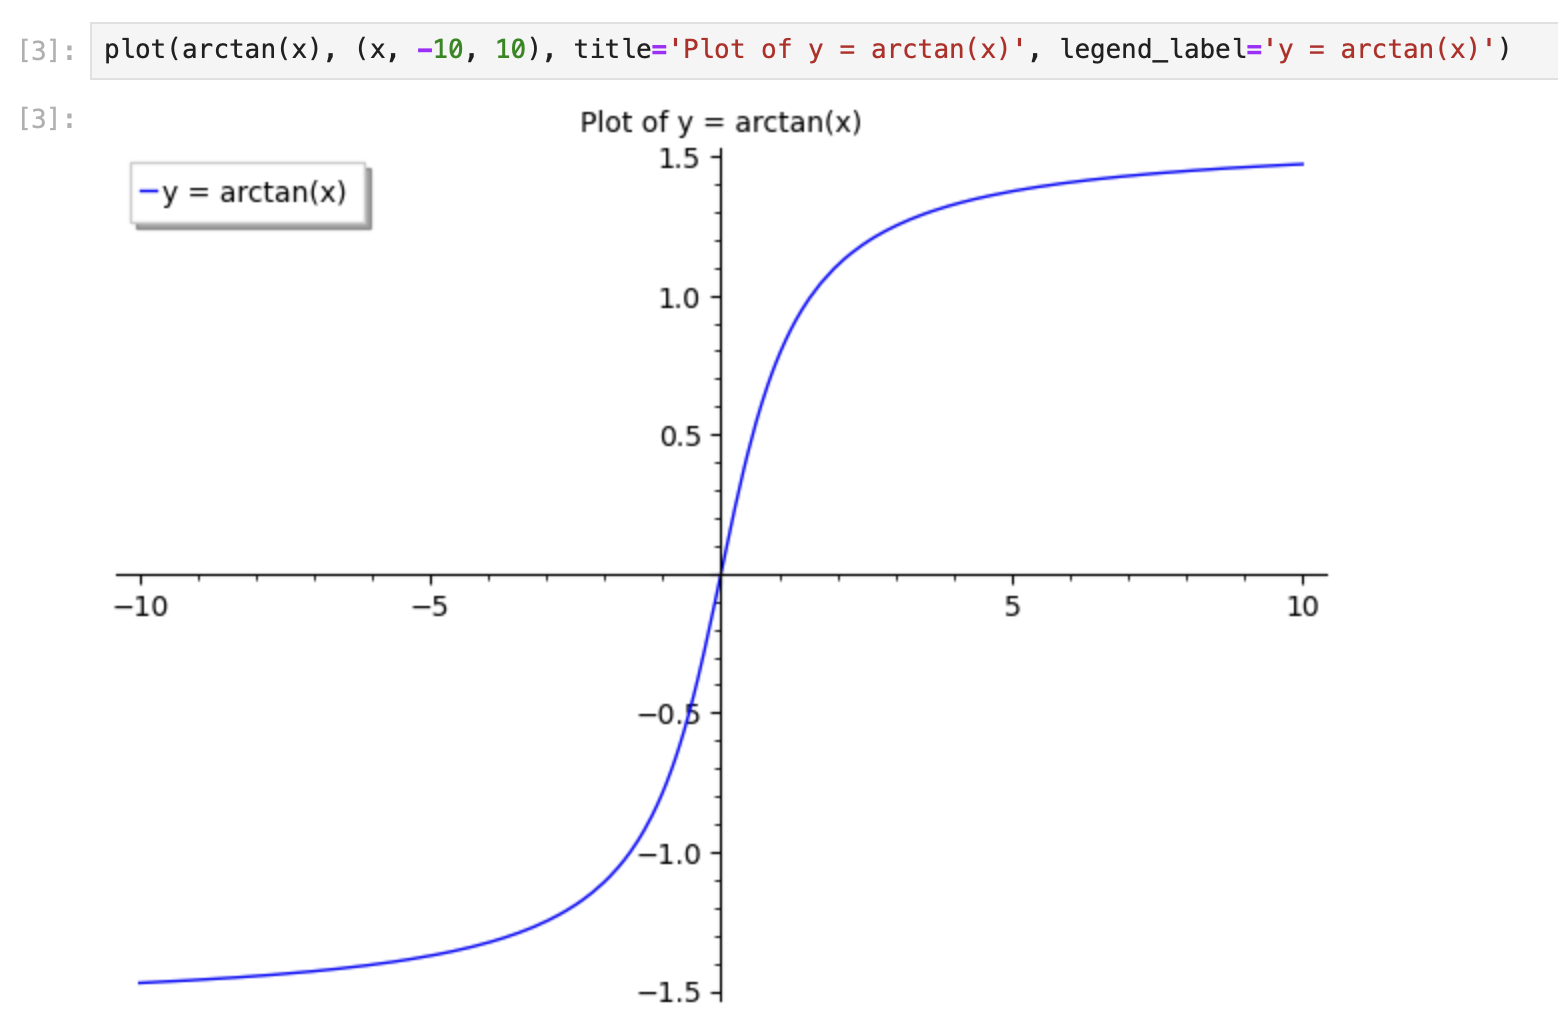
\includegraphics[height=8cm,width=15cm]{pdehw1}
   \end{minipage}
\end{center}
\end{proof}
\begin{theorem}
\begin{align}
\label{he2}
\text{ Solve }au_x+b u_y +cu=0
\end{align}
\end{theorem}
\begin{proof}
Fix 
\begin{align*}
\begin{cases}
  x'\triangleq ax+by \\
  y'\triangleq bx-ay
\end{cases}
\end{align*}
This map is clearly a diffeomorphism. Compute 
\begin{align*}
  \begin{cases}
    u_x= \frac{\partial u}{\partial x'}\frac{\partial x'}{\partial x}+\frac{\partial u}{\partial y'}\frac{\partial y'}{\partial x}=au_{x'}+bu_{y'}\\
    u_y=\frac{\partial u}{\partial x'}\frac{\partial x'}{\partial y}+\frac{\partial u}{\partial y'}\frac{\partial y'}{\partial y}=bu_{x'}-au_{y'}
  \end{cases}
\end{align*}
Plugging it back into the PDE in \myref{Equation}{he2}, we have 
\begin{align}
\label{he3}
cu+ (a^2+b^2)u_{x'}=0
\end{align}
If $c=a^2+b^2=0$, then all smooth functions are solution. If $a^2+b^2=0$ but $c\neq 0$, then clearly the only solution is $u=\tilde{0} $. If $a^2+b^2\neq 0$ but $c=0$, then $u_{x'}=\tilde{0}$, which implies $u=f(y')$ where $y'=bx-ay$ and  $f$ can be arbitrary smooth function.\\

Now, suppose $a^2+b^2\neq 0\neq c$, note that the PDE in \myref{Equation}{he3} is just an ODE of the form 
\begin{align*}
y+\frac{a^2+b^2}{c}y'=0
\end{align*}
The general solution to this ODE is 
\begin{align*}
y=Ce^{\frac{-ct}{a^2+b^2}}
\end{align*}
In other words, the general solution of the PDE in \myref{Equation}{he3} is 
\begin{align*}
u=C e^{\frac{-cx'}{a^2+b^2}}=Ce^{\frac{-c(ax+by)}{a^2+b^2}}
\end{align*}


\end{proof}
\section{PDE HW 2}
\begin{question}{}{}
Consider hear flow in a long circular cylinder where the temperature depends only on $t$ and on the distance $r$ to the axis of the cylinder. Here $r=\sqrt{x^2+y^2}$ is the cylindrical coordinate. From the three dimensional hear equation derive the equation $u_t=k (u_{rr}+\frac{u_r}{r})$
\end{question}
\begin{proof}
Write the three dimensional hear equation by 
\begin{align*}
u_t= k \Delta u
\end{align*}
Note that the Laplacian $\Delta u$ when written in cylindrical coordinate is 
\begin{align*}
\Delta u= u_{rr} + \frac{u_r}{r} +\frac{u_{\theta \theta}}{r^2} + u_{zz}
\end{align*}
Because the premise says that $u$ is constant in $z$ and  $\theta$, we know $u_{\theta \theta}=u_{zz}=0$
\begin{align*}
\Delta u = u_{rr}+ \frac{u_r}{r}
\end{align*}
This give us 
\begin{align*}
u_t= k (u_{rr}+ \frac{u_r}{r})
\end{align*}
\end{proof}
\section{PDE HW 3}
\begin{question}{}{}
Find a solution of 
\begin{align*}
\begin{cases}
  u_t=u_{xx}\\
  u(x,0)=x^2
\end{cases}
\end{align*}
\end{question}
\begin{proof}
Clearly $u=x^2+2t$ suffices.
\end{proof}
\begin{question}{}{}
Consider the ODE 
\begin{align*}
\begin{cases}
  u''+u'=f \\
  u'(0)=u(0)=\frac{1}{2}(u'(l)+u(l))
\end{cases}
\end{align*}
where $f$ is given. 
\begin{enumerate}[label=(\alph*)]
  \item Is the solution unique? 
  \item Does a solution necessarily exist, or is there a condition that $f$ must satisfy for existence? 
\end{enumerate}
\end{question}
\begin{proof}
The solution space of linear homogeneous ODE $u''+u'=0$  is spanned by $e^{-x}$ and constant. If we add in the initial condition  $u'(0)=u(0)$, then the solution space become the subspace spanned by $e^{-x}-2$. One can check that if $u \in\operatorname{span}(e^{-x}-2)$, then 
\begin{align*}
u(0)=\frac{1}{2}(u'(l)+u(l))\text{ for all $l\inr$ }
\end{align*}
We now know the solution of the original ODE is not unique, since any solution added by $e^{-x}-2$ is again a solution. \\

Integrating both side on $[0,l]$, we see that given the boundary conditions, $f$ must satisfy 
\begin{align*}
\int_0^l f(x)dx&=\int_0^l u''+u'dx\\
&=u(l)+u'(l)-u(0)-u'(0)=0
\end{align*}
\end{proof}
\begin{question}{}{}
Find the regions in the $xy$ plane where the equation 
 \begin{align*}
   (1+x)u_{xx}+2xyu_{xy}-y^2u_{yy}=0
\end{align*}
is elliptic, hyperbolic, or parabolic. Sketch them. 
\end{question}
\begin{proof}
The discriminant is exactly 
\begin{align*}
  (xy)^2- (1+x)(-y^2)&=x^2y^2+xy^2+y^2\\
  &=y^2 (x^2+x+1)\\
  &=y^2[(x+\frac{1}{2})^2+ \frac{3}{4}]
\end{align*}
It then follows that the equation is parabolic if and only if $y=0$, and hyperbolic if and only if  $y\neq 0$. 

\end{proof}
\section{PDE HW 4}
\begin{question}{}{}
Solve 
\begin{align*}
\begin{cases}
  u_{tt}=c^2u_{xx} \\
  u(x,0)=e^x \\
  u_t(x,0)= \sin x 
\end{cases}
\end{align*}
\end{question}
\begin{proof}
Let 
\begin{align*}
u\triangleq f(x+ct)+g(x-ct)
\end{align*}
Plugging the initial conditions, we know 
\begin{align*}
\begin{cases}
 f(x)+g(x)=e^x \\
 f'(x)-g'(x)= \frac{\sin x}{c} 
\end{cases}
\end{align*}
This give us 
\begin{align*}
f'(x)= \frac{e^x+ \frac{\sin x}{c}}{2}\text{ and }g'(x)= \frac{e^x - \frac{\sin x}{c}}{2}
\end{align*}
Then by FTC, we have
\begin{align*}
\begin{cases}
  f(x)= \frac{e^x-\frac{\cos x}{c}}{2}+f(0)- \frac{1}{2} +\frac{1}{2c} \\
  g(x)= \frac{e^x + \frac{\cos x}{c}}{2} +g(0) - \frac{1}{2}- \frac{1}{2c}
\end{cases}
\end{align*}
Note that $f(0)+g(0)=e^0=1$, which cancel the constant terms in $u$, i.e.
\begin{align*}
u&=f(x+ct)+g(x-ct)\\
&=\frac{e^{x+ct}+ e^{x-ct} + \frac{-\cos (x+ct)+ \cos (x-ct)}{c}}{2}
\end{align*}
\end{proof}
\begin{question}{}{}
Solve 
\begin{align*}
\begin{cases}
u_{xx}+u_{xt}-20u_{tt}=0 \\
u(x,0)=\phi (x) \\
u_t(x,0)= \psi (x)
\end{cases}
\end{align*}
\end{question}
\begin{proof}
The PDE can be write in the form of 
\begin{align*}
  (\partial_x + 5\partial_t) (\partial_x - 4 \partial _t)u=0
\end{align*}
which have the general solution 
\begin{align*}
u(x,t)=f(5x-t)+g(4x+t)
\end{align*}
We now see 
\begin{align*}
f(5x)+g(4x)=\phi (x)\text{ and }-f'(5x)+g'(4x)=\psi (x)
\end{align*}
This then give us 
\begin{align*}
f'(5x)=\frac{(\phi' - 4\psi)(x)}{9}\text{ and }g'(4x)= \frac{(\phi '+5\psi )(x)}{9}
\end{align*}
and thus 
\begin{align*}
f(x)&=f(0)+ \int_0^x f'(s)ds\\
&=f(0)+\int_0^x \frac{(\phi' -4\psi)(\frac{s}{5})}{9}ds \\
&=f(0)+ \frac{5}{9}\Big[\phi (\frac{x}{5})-\phi (0) \Big] - \frac{4}{9}\int_0^x \psi (\frac{s}{5})ds
\end{align*}
and similarly 
\begin{align*}
g(x)&=g(0)+\int_0^x g'(s)ds \\
&=g(0)+ \int_0^x \frac{(\phi ' +5 \psi )(\frac{s}{4})}{9}ds \\
&=g(0)+ \frac{4}{9}\Big[ \phi (\frac{x}{4})- \phi (0) \Big]+\frac{5}{9} \int_0^x \psi (\frac{s}{4})ds
\end{align*}
Noting that $f(0)+g(0)=u(0,0)=\psi (0)$, we now have
\begin{align*}
u(x,t)&=f(5x-t)+g(4x+t) \\
&=\frac{5\phi (\frac{5x-t}{5})+4 \phi (\frac{4x+t}{4})}{9} - \frac{4}{9}\int_0^{5x-t}\psi (\frac{s}{5})ds + \frac{5}{9}\int_0^{4x+t}\psi (\frac{s}{4})ds
\end{align*}
\end{proof}
\section{PDE HW 5}
\begin{question}{}{}
Solve 
\begin{align*}
&u_t=ku_{xx}\\
&u(x,0+)=e^{-x}\\
&u(0+,t)=0
\end{align*}
on the half line $0<x<\infty$
\end{question}
\begin{proof}
Extend the initial condition to 
\begin{align*}
\phi_{\operatorname{odd}}(x)\triangleq \begin{cases}
  e^{-x}& \text{ if $x>0$ }\\
  0& \text{ if $x=0$ }\\
  -e^{x}& \text{ if $x<0$ }
\end{cases}
\end{align*}
We then solve 
\begin{align*}
u(x,t)&=\frac{1}{2\sqrt{\pi kt} }\int_{\R} e^{\frac{-(x-y)^2}{4kt}}\phi_{\operatorname{odd}}(y)dy\\
&=\frac{1}{2 \sqrt{\pi kt} }\Big[\int_0^\infty e^{\frac{-(x-y)^2}{4kt}}e^{-y}dy - \int_{-\infty}^0 e^{\frac{-(x-y)^2}{4kt}}e^ydy  \Big] \\
&=\frac{1}{2 \sqrt{\pi kt} }\Big[\int_0^{\infty}e^{\frac{-(y-(x-2kt))^2-4ktx+4k^2t^2}{4kt}}dy -\int^{0}_{-\infty}e^{\frac{-(y-(x+2kt))^2+4ktx+4k^2t^2}{4kt}}dy  \Big] \\
&=\frac{1}{2 \sqrt{\pi kt} }\Big[e^{-x+kt}\int_0^{\infty}e^{\frac{-(y-(x-2kt))^2}{4kt}}dy -e^{x+kt}\int^{0}_{-\infty}e^{\frac{-(y-(x+2kt))^2}{4kt}}dy  \Big]  \\
&=\frac{1}{\sqrt{\pi} }\Big[e^{-x+kt}\int_{\frac{2kt-x}{2\sqrt{kt} }}^{\infty}e^{-p^2}dp -e^{x+kt}\int_{-\infty}^{\frac{-2kt-x}{2\sqrt{kt} }}e^{-p^2}dp \Big]\\
&=\frac{1}{\sqrt{\pi} }\Big[e^{-x+kt}\Big( \frac{\sqrt{\pi} }{2}- \frac{2}{\sqrt{\pi}}\operatorname{erf}(\frac{2kt-x}{2\sqrt{kt} })   \Big)-e^{x+kt}\Big( \frac{\sqrt{\pi} }{2}- \frac{2}{\sqrt{\pi} }\operatorname{erf}( \frac{2kt+x}{2\sqrt{kt}}) \Big) \Big]
\end{align*}
\end{proof}
\section{PDE HW 6}
\begin{question}{}{}
Solve $u_{tt}=4u_{xx}$ for $0<x<\infty,u(0,t)=0,u(x,0)=1,u_t(x,0)=0$ using the reflection method. The solution has a singularity find its location. 
\end{question}
\begin{proof}
Define 
\begin{align*}
\phi (x)\triangleq \begin{cases}
  1& \text{ if $x>0$ }\\
  -1& \text{ if $x<0$ }
\end{cases}\text{ and }\psi (x)\triangleq 0
\end{align*}
We are required to solve the following Dirichlet's problem for wave equation 
\begin{align*}
u_{tt}=4u_{xx}\text{ for }-\infty < x< \infty \\
u(x,0)=\phi (x)\text{ and }u_t(x)=\psi (x)
\end{align*}
The solution is exactly 
\begin{align*}
u(x,t)&=\frac{\phi(x+2t)+\phi (x-2t)}{2}+\int_{x-2t}^{x+2t} \psi (s)ds \\
&=\frac{\phi (x+2t)+\phi (x-2t)}{2}\\
&=\begin{cases}
  1& \text{ if $x-2t>0$ }\\
  0& \text{ if  }x+2t>0>x-2t\\
  -1& \text{ if  }0>x+2t
\end{cases}
\end{align*}
On the half line, the solution is 
\begin{align*}
u(x,t)=\begin{cases}
  1& \text{ if $x-2t>0$ }\\
  0& \text{ if $x-2t<0$ }
\end{cases}
\end{align*}
So the singularity is exactly on the line $x-2t=0$ 
\end{proof}
\begin{question}{}{}
Solve the inhomogeneous Neumann diffusion problem on the half-line
\begin{align*}
\begin{cases}
  w_t-kw_{xx}=0\text{ for }x\in (0,\infty)\text{ \textbf{(Homogeneous DE)}}\\
  w_x(0,t)=h(t)\text{ \textbf{(Non-homogeneous BC)} }\\
  w(x,0)= \phi (x) \text{ \textbf{(IC)} }
\end{cases}
\end{align*}
by the subtraction method indicated in the text.
\end{question}
\begin{proof}
Suppose $w$ is a solution to our problem. If we define 
\begin{align*}
u(x,t)\triangleq w(x,t)-xh(t)\text{ for }x\in (0,\infty)
\end{align*}
We see that $u$ satisfy 
\begin{align*}
\begin{cases}
  u_t-ku_{xx}=-xh'(t)\text{ for }x\in (0,\infty)\text{ \textbf{(Non-homogeneous DE)} }\\
  u_x(0,t)=0\text{ \textbf{(Good BC)} }\\
  u(x,0)=\phi (x)-xh(0)\text{ \textbf{(IC)} }
\end{cases}
\end{align*}
Define 
\begin{align*}
f_{\operatorname{even}}(x,t)\triangleq \begin{cases}
  -xh'(t)& \text{ if $x>0$ }\\
  xh'(t)& \text{ if $x<0$ }
\end{cases}
\end{align*}
And define 
\begin{align*}
\phi_{\operatorname{even},*}\triangleq \begin{cases}
  \phi (x)-xh(0)& \text{ if $x>0$ }\\
  \phi (-x)+xh(0)& \text{ if $x<0$ }
\end{cases}
\end{align*}
And define 
\begin{align*}
u_{\operatorname{even}}(x,t)\triangleq \int_{\R}S(x-y)\phi_{\operatorname{even,*}}(y)dy+\int_0^t \int_{\R}S(x-y,t-s)f_{\operatorname{even}}(y,s)dyds
\end{align*}
It then follows that $u_{\operatorname{even}}$ solve the non-homogeneous DE and IC. To see that $u_x(0,t)=0$, one simply observe that $u$ is even in  $x$. The solution to the original problem is then 
\begin{align*}
w(x,t)\triangleq u_{\operatorname{even}}(x,t)+xh(t)\text{ for }x\in (0,\infty)
\end{align*}
\end{proof}
\section{PDE HW 7}
\begin{question}{}{}
Solve 
\begin{align*}
\begin{cases}
  u_{tt}=c^2u_{xx}\text{ for }x\in (0,\infty)\text{ \textbf{(Homogeneous DE)} } \\
  u(x,0)=x,u_t(x,0)=0\text{ \textbf{(IC)} }\\
  u(0,t)=t^2\text{ \textbf{(BC)} }
\end{cases}
\end{align*}
\end{question}
\begin{proof}
If we define 
\begin{align*}
w=u-t^2
\end{align*}
we see that $w$ satisfy 
\begin{align*}
\begin{cases}
  w_{tt}-c^2w_{xx}=-2\text{ for }x\in (0,\infty)\text{ \textbf{(Non-homogeneous DE)} } \\
  w(x,0)=x,w_t(x,0)=0\text{ \textbf{(IC)} }\\
  w(0,t)=0\text{ \textbf{(Dirichlet BC)} }
\end{cases}
\end{align*}
then if we define 
\begin{align*}
\phi_{\operatorname{odd}}(x)\triangleq x\text{ and }f_{\operatorname{odd}}(x,t)\triangleq \begin{cases}
  -2& \text{ if $x>0$ }\\
  2& \text{ if $x<0$ }
\end{cases} 
\end{align*}
and 
\begin{align*}
  w(x,t)&\triangleq  \frac{\phi (x+ct)+ \phi (x-ct)}{2} + \frac{1}{2c}\int_0^t \int^{x+c(t-s)}_{x-c(t-s)} f_{\operatorname{odd}}(y,s)dyds  \\
  &= x+  \begin{cases}
   -t^2& \text{ if $x-ct>0$ }\\
    \frac{x^2}{c^2}-\frac{2tx}{c}& \text{ if $x-ct<0$ }
  \end{cases}
\end{align*}
Note that we only consider when $x\geq 0$. This then give us 
\begin{align*}
u(x,t)= \begin{cases}
  x &\text{ if $x-ct>0$ }\\
  x+ (t-\frac{x}{c})^2 &\text{ if $x-ct<0$ }
\end{cases}
\end{align*}
\end{proof}
\section{PDE HW 8}
\begin{question}{}{}
Solve the Schrodinger equation 
\begin{align*}
\begin{cases}
  u_t=iku_{xx}\text{ for }0<x<l\text{ \textbf{(Homogeneous DE)} } \\
  u_x(0,t)=u(l,t)=0\text{ \textbf{(BC)} }
\end{cases}
\end{align*}
for real $k \in (0,l)$. 
\end{question}
\begin{proof}
Again we do the separation of the variables 
\begin{align*}
u\triangleq T(t)X(x)
\end{align*}
Some tedious efforts shows that $u$ is a solution of this original question as long as $X,T$ satisfy the following ODE 
\begin{align*}
\begin{cases}
  X''(x)+\ld  X(x)=0\\
  X'(0)=X(l)=0
\end{cases}\text{ and }T'(t)+\ld  ik T(t)=0
\end{align*}
where $\ld \inc$ is arbitrary constant. The solution of the second ODE is obviously 
\begin{align*}
T(t)\triangleq Ce^{-\ld  ik t}
\end{align*}
where $C\inc$ is arbitrary constant. It remains to find what values can $\ld $ take so that $X$ has non-trivial solutions.  If $\ld =0$, then to satisfy the ordinary differential equation, the solution must take the forms $X=C+Dx$, where $C,D\inc$ are arbitrary constant. Plugging the initial conditions, we see that $C=D=0$. In other words, if  $\ld =0$, then $X$ can only be trivial. If $\ld \neq 0$, ODE of $X$ suggest that  $X$ must take the form
\begin{align*}
X\triangleq Ae^{\gamma x}+Be^{-\gamma x}
\end{align*}
where $\gamma \inc$ satisfy $\gamma ^2=-\ld $. Plug in $X'(0)=0$, we see 
\begin{align*}
0=\gamma (A-B)
\end{align*}
which implies $A=B$. Plug in $X(l)=0$, we see 
\begin{align*}
0=A e^{\gamma  l}+B e^{- \gamma l}=A(e^{\gamma l}+e^{-\gamma l})
\end{align*}
Then for $X$ to be non-trivial, we must have  
 \begin{align*}
e^{\gamma l}+e^{-\gamma l} =0
\end{align*}
By periodicity property of exponential function, we then can deduce
\begin{align*}
\gamma = \frac{ i \pi(2n+1)}{l}\text{ and }\ld = \frac{(2n+1)^2\pi ^2}{l^2}
\end{align*}
It then follows from $X=Ae^{\gamma x}+Be^{-\gamma x}$ that 
\begin{align*}
X&= (A+B) \cos \Big(\frac{\pi (2n +1) x}{l}\Big)+ (A-B)i\sin \Big(\frac{ \pi (2n+1)x}{l}\Big)\\
&=(A+B) \cos \Big(\frac{ \pi (2n+1) x}{l}\Big)\hspace{0.5cm}(\because A=B)
\end{align*}
\end{proof}
\section{PDE HW 9}
\begin{question}{}{}
Find the full Fourier series of $e^x$ on  $(-l,l)$ in its real and complex forms. (Hint: It is convenient to find the complex form first)
\end{question}
\begin{proof}
Write 
\begin{align*}
e^x= \sum_{n=- \infty}^{\infty} c_n e^{ \frac{i n \pi x }{l}}
\end{align*}
Compute 
\begin{align*}
c_n&= \frac{1}{2l}\int_{-l}^{l}e^x e^{\frac{- i n \pi  x}{l}}dx \\
&=\frac{1}{2l}\int_{-l}^{l}e^{ \frac{(l-i n\pi )x}{l}}dx\\
&=\frac{1}{2l} \cdot \frac{le^{\frac{(l-i n \pi )x}{l}}}{l-i n \pi  }\Big|_{x=-l}^{l} \\
&= \frac{l(e^{l- i n \pi }- e^{-(l- i n \pi )})}{2l (l- i n \pi )}\\
&= \frac{(-1)^n (e^l - e^{-l})}{2(l - i n \pi )}= \frac{(-1)^n}{(l- i n \pi )}\sinh (l)
\end{align*}
We now have 
\begin{align*}
e^x&= \sum_{n=-\infty}^{\infty} \frac{(-1)^n}{(l- i n \pi )}\sinh (l) e^{\frac{i n \pi x}{l}} \\
&= \frac{\sinh (l)}{l}+ \sum_{n=1}^{\infty} \Big[\frac{(-1)^n \sinh (l) }{(l- i n \pi )}e^{\frac{i n \pi  x}{l}}+ \frac{(-1)^n \sinh (l)}{(l+ i n \pi )}e^{\frac{- i n \pi x}{l}}  \Big] \\
&=\frac{\sinh (l)}{l}+ \sum_{n=1}^{\infty} (-1)^n\sinh (l) \Big[ \frac{\cos (\frac{n \pi  x}{l})+ i \sin (\frac{n \pi  x}{l})}{l- i n \pi }+ \frac{\cos (\frac{n \pi  x}{l})- i \sin (\frac{n \pi  x}{l})}{l+ i n \pi } \Big]\\
&= \frac{\sinh (l)}{l}\\
&+ \sum_{n=1}^{\infty} (-1)^n \sinh (l) \cdot \frac{(l+ i n \pi )\big(\cos (\frac{n \pi  x}{l})+i \sin (\frac{n \pi  x}{l})  \big)+(l- i n \pi )\big( \cos (\frac{n \pi  x}{l})- i \sin (\frac{n \pi  x}{l}) \big)}{l^2 + n^2 \pi ^2} \\
&=\frac{\sinh (l)}{l}+ \sum_{n=1}^{\infty} \frac{(-1)^n \sinh (l)\big[ 2l \cos (\frac{n \pi  x}{l})-2n \pi  \sin (\frac{n \pi  x}{l}) \big]}{l^2+n^2\pi  ^2} \\
&= \sum_{n=0}^{\infty} \frac{2(-1)^n \sinh (l)}{l^2 + n^2 \pi ^2}\Big[l\cos (\frac{n \pi  x}{l})- n \pi  \sin (\frac{n \pi  x}{l}) \Big]
\end{align*}

\end{proof}

\begin{question}{}{}
Find the complex eigenvalues of the first-derivative operator $\frac{d}{dx}$ subject to the single boundary condition $X(0)=X(1)$. Are the eigenfunctions orthogonal on the interval $(0,1)$? 
\end{question}
\begin{proof}
We are solving the eigenproblem 
\begin{align*}
\begin{cases}
  X'+ \ld X=0 \\
  X(0)=X(1)
\end{cases}
\end{align*}
Clearly, the solution $X$ must take the form  $X=e^{-\ld x}$. The boundary conditions then implies 
\begin{align*}
e^{-\ld }=X(1)=X(0)=1
\end{align*}
which implies 
\begin{align*}
\ld = 2n i \pi \text{ for }n\inz
\end{align*}
Compute for distinct $n,m$ 
\begin{align*}
\langle X_n,X_m\rangle = \int_0^1 e^{- 2(n-m) i \pi  x}dx= \frac{e^{-2(n-m)i \pi  x}}{-2(n-m)i \pi }\Big|_{x=0}^1= 0
\end{align*}
So the eigenfunctions are indeed orthogonal. 
\end{proof}
\chapter{Differential Geometry HW} 
\section{HW1} 
\begin{abstract}
In this HW, we give precise definition to $\P^n$  and $\RP^n$, and we rigorously show
\begin{enumerate}[label=(\alph*)]
  \item $\RP^n$  has a smooth structure. 
  \item $\P^n$ is homeomorphic to $\RP^n$ 
   \item $\P^n$ has a smooth structure.
\end{enumerate}
We also solved  \customref{othq}{the other two questions}. Note that in this PDF, brown text is always a clickable hyperlink reference.  
\end{abstract}
\begin{mdframed}
Define an equivalence relation on $\R^{n+1}\setminus \set{\textbf{0}}$ by 
\begin{align*}
\textbf{x}\sim \textbf{y}\overset{\triangle}{\iff }\textbf{y}=\ld \textbf{x}\text{ for some $\ld \inr^*$ } 
\end{align*}
Let $\RP ^n\triangleq (\R^{n+1}\setminus \set{\textbf{0}})\setminus \sim $ be the quotient space and let  
\begin{align*}
V_i\triangleq \set{\textbf{x}\inr^{n+1}:\textbf{x}^i \neq 0}\text{ for each }1\leq i\leq n+1
\end{align*}
By definition, it is clear that 
\begin{align*}
\text{ either }\pi^{-1}(\pi (\textbf{x}))\subseteq V_i\text{ or }\pi^{-1}(\pi (\textbf{x}))\subseteq V_i^c
\end{align*}
Then if we define $\phi_i:V_i\rightarrow \R^n$ by
\begin{align*}
\phi_i(\textbf{x})\triangleq \Big(\frac{\textbf{x}^1}{\textbf{x}^i},\dots ,\frac{\textbf{x}^{i-1}}{\textbf{x}^i},\frac{\textbf{x}^{i+1}}{\textbf{x}^i},\dots,\frac{\textbf{x}^{n+1}}{\textbf{x}^i} \Big)
\end{align*}
because $\pi (\textbf{x})=\pi(\textbf{y})\implies \phi_i(\textbf{x})=\phi_i(\textbf{y})$, we can well induce a map 
\begin{align*}
\Phi_i:U_i\triangleq \pi (V_i)\subseteq \R P^n\rightarrow \R^n; \pi (\textbf{x})\mapsto \phi_i(\textbf{x})
\end{align*}
Note that one has the equation 
\begin{align*}
\Phi_i(\pi (\textbf{x}))= \phi_i(\textbf{x})\text{ for all }\textbf{x}\in V_i
\end{align*}
\end{mdframed}
\begin{theorem}
\textbf{(Real Projective Space with a differentiable atlas)} We have
\begin{align*}
  \R P^n\text{ with atlas }\set{(U_i,\Phi_i):1\leq i\leq n+1}\text{ is a differentiable manifold }
\end{align*}
\end{theorem}
\begin{proof}
We are required to prove 
\begin{enumerate}[label=(\alph*)] 
  \item $(U_i,\Phi_i)$ are all charts. 
  \item $\set{(U_i,\Phi_i):1\leq i\leq n+1}$ form a differentiable atlas. 
\item $\R P^n$ is Hausdorff.
\item $\R P^n$ is second-countable. 
\end{enumerate}
 Because $\pi^{-1}(U_i)=V_i$ and $V_i$ is clearly open in $\R^{n+1}\setminus \set{\textbf{0}}$, we know $U_i\subseteq \R P^n$ is open. Note that clearly,   $\Phi_i(U_i)=\R^n$. To show $(U_i,\Phi_i)$ is a chart, it remains to show that $\Phi_i$ is a homeomorphism between $U_i$ and  $\R^n$.  It is straightforward to check $\Phi_i$ is one-to-one on $U_i$. This implies $\Phi_i$ is a bijective between $U_i$ and  $\R^n$. \\


Fix open $E\subseteq \R^n$. We see 
\begin{align*}
  \pi^{-1}(\Phi_i^{-1}(E))=\phi_i^{-1}(E)
\end{align*}
Then because $\phi_i:V_i\rightarrow \R^n$ is clearly continuous, we see $\phi_i^{-1}(E)$ is open in $\R^{n+1}\setminus \set{\textbf{0}}$, and it follows from definition of quotient topology  $\Phi_i^{-1}(E)\subseteq \R P^n$ is open. Then because $U_i$ is open in  $\R P^n$, we see $\Phi_i^{-1}(E)$ is open in $U_i$. We have proved  $\Phi_i:U_i\rightarrow \R^n$ is continuous.\\


Define $\Psi_i: \R^n\rightarrow V_i$ by 
\begin{align*}
\Psi (\textbf{x}^1,\dots ,\textbf{x}^n)= (\textbf{x}^1,\dots ,\textbf{x}^{i-1},1,\textbf{x}^i,\dots ,\textbf{x}^n)
\end{align*}



Observe that for all $\textbf{x}\in \Phi_i(U_i)$, we have
\begin{align*}
\Phi_i^{-1}(\textbf{x})= \pi(\Psi_i (\textbf{x}))
\end{align*}
It then follows from $\Psi_i:\R^n\rightarrow V_i$ and $\pi:\R^{n+1}\setminus \set{\textbf{0}}\rightarrow \R P^n$ are continuous that $\Phi_i^{-1}:\R^n\rightarrow \R P^n$ is continuous.\\

We have proved that $(\Psi_i,U_i)$ are all charts. Now, because $V_i$ clearly cover $\R^{n+1}$, we know $U_i$ also cover  $\R P^n$. We have proved $\set{(U_i,\Phi):1\leq i\leq n+1}$ form an atlas. The fact $\R P^n$ is second-countable follows. \\

Fix $(\textbf{x}_1,\dots ,\textbf{x}_{n})\in \Phi_i(U_i\cap U_j)$. We compute 
\begin{align*}
\Phi_j\circ \Phi_i^{-1} (\textbf{x}^1,\dots ,\textbf{x}^{n} )&=\Phi_j \Big( [(\textbf{x}^1,\dots ,\textbf{x}^{i-1},1,\textbf{x}^i,\textbf{x}^{i+1},\dots, \textbf{x}^n)] \Big) \\
&= \begin{cases}
  (\frac{\textbf{x}^1}{\textbf{x}^j},\dots , \frac{\textbf{x}^{j-1}}{\textbf{x}^j},\frac{\textbf{x}^{j+1}}{\textbf{x}^j},\dots ,\frac{\textbf{x}^{i-1}}{\textbf{x}^j},\frac{1}{\textbf{x}^j},\frac{\textbf{x}^i}{\textbf{x}^j},\dots ,\frac{\textbf{x}^n}{\textbf{x}^j})& \text{ if $j<i$ }\\
  (\frac{\textbf{x}^1}{\textbf{x}^{j-1}},\dots , \frac{\textbf{x}^{i-1}}{\textbf{x}^{j-1}},\frac{1}{\textbf{x}^{j-1}},\frac{\textbf{x}^i}{\textbf{x}^{j-1}},\dots , \frac{\textbf{x}^{j-2}}{\textbf{x}^{j-1}}, \frac{\textbf{x}^j}{\textbf{x}^{j-1}}, \dots,\frac{\textbf{x}^n}{\textbf{x}^{j-1}})& \text{ if $j>i$ }
\end{cases}
\end{align*}
This implies our atlas is indeed differentiable. \\

Before we prove $\RP^n$ is Hausdorff, we first prove that  \olive{$\pi:\R^{n+1}\setminus \set{\textbf{0}}\rightarrow \RP^n$ is an open mapping}. Let $U\subseteq \R^{n+1}\setminus \set{\textbf{0}}$ be open. Observe that 
\begin{align*}
\pi^{-1}(\pi(U))= \set{t\textbf{x}\inr^{n+1}:t\neq 0\text{ and }\textbf{x}\in U}
\end{align*}
Fix $t_0\textbf{x}\in \pi^{-1}(\pi (U))$. Let $B_\epsilon (\textbf{x})\subseteq U$. Observe that
\begin{align*}
B_{\abso{t_0}\epsilon }(t_0\textbf{x})\subseteq t_0B_\epsilon (\textbf{x})\subseteq t_0U\subseteq \pi^{-1}(\pi (U))
\end{align*}
This implies $\pi ^{-1}(\pi (U))$ is open.  $\odone$ \\

Now, \customref{Hausdorff and Quotient}{because $\pi$ is open, to show $\RP^n$ is Hausdorff, we only have to show}
 \begin{align*}
R_\pi \triangleq \set{(\textbf{x},\textbf{y})\in (\R^{n+1}\setminus \set{\textbf{0}})^2:\pi (\textbf{x})= \pi (\textbf{y})}\text{ is closed }
\end{align*}
Define $f:(\R^{n+1}\setminus \set{\textbf{0}})^2\rightarrow \R$ by 
\begin{align*}
f(\textbf{x},\textbf{y})\triangleq \sum_{i\neq j} (\textbf{x}^i\textbf{y}^j-\textbf{x}^j \textbf{y}^i)^2
\end{align*}
Note that $f$ is clearly continuous and $f^{-1}(0)=R_\pi$, which finish the proof.
\end{proof}
\begin{mdframed}
Alternatively, we can characterize $\R P^n$ by identifying the antipodal pints on $S^n\triangleq \set{\textbf{x}\inr^{n+1}:\abso{\textbf{x}}=1}$ as one point 
\begin{align*}
\textbf{x}\sim \textbf{y}\overset{\triangle}{\iff } \textbf{x}=\textbf{y}\text{ or }\textbf{x}=-\textbf{y}
\end{align*}
and let $\P^n\triangleq S^n\setminus \sim $ be the quotient space.
\end{mdframed}
\begin{theorem}
\label{RPnhom}
\textbf{(Equivalent Definitions of Real Projective Space)} 
\begin{align*}
\RP^n\text{ and }\P^n\text{ are homeomorphic }
\end{align*}
\end{theorem}
\begin{proof}
Define $F:\P^n\rightarrow \RP^n$ by 
\begin{align*}
\set{\textbf{x},-\textbf{x}}\mapsto \set{\ld  \textbf{x}:\ld \inr^*}
\end{align*}
It is straightforward to check that $F$ is well-defined and bijective. Define $f:S^n \rightarrow \R P^n$ by 
\begin{align*}
f= \pi \circ \textbf{id}
\end{align*}
where $\textbf{id}:S^n \rightarrow \R^{n+1}\setminus \set{\textbf{0}}$ and $\pi:\R^{n+1}\setminus \set{\textbf{0}}\rightarrow \R P^n$ are continuous. Check that  
\begin{align*}
f=F\circ p
\end{align*}
where $p:S^n\rightarrow \P^n$ is the quotient mapping. It now follows from the \customref{quotient property}{universal property} that $F$ is continuous, and since $\P^n$ is compact and  $\R P^n$ is Hausdorff,  it also follows that  \customref{HbC}{$F$ is a homeomorphism between $\R P^n$ and  $\P^n$}. 
\end{proof}
\begin{mdframed}
Knowing that $F:\P^n\rightarrow \RP^n$ is a homeomorphism and $\RP^n$ is a smooth manifold, we see that  $\P^n$ is Hausdorff and second-countable, and if we define the atlas 
\begin{align*}
  \set{(F^{-1}(U_i), \Phi_i \circ F):1\leq i\leq n+1}
\end{align*}
We see this atlas is indeed smooth, since 
\begin{align*}
  (\Phi_i\circ F)\circ (\Phi_j \circ F)^{-1}=\Phi_i \circ \Phi_j^{-1}
\end{align*}
\end{mdframed}
\begin{question}{}{}
\label{othq}
Let $X$ be a set equipped with
\begin{enumerate}[label=(\alph*)]
  \item a collection $(U_\alpha )_{\alpha  \in I}$ of subsets that covers $X$. 
  \item a collection of bijection $\phi_\alpha  : U_\alpha \rightarrow \phi_\alpha (U_\alpha )$ that maps $U_\alpha $ to an open subset $\phi _\alpha (U_\alpha )$ of $\R^n$. 
  \item For each $\alpha ,\beta \in I $, the set $\phi_\alpha (U_\alpha \cap U_\beta )$ is open. 
  \item For each $\alpha ,\beta \in I, \phi_\beta \circ \phi_\alpha ^{-1}:\phi_\alpha (U_\beta  \cap U_\alpha )\rightarrow \phi_\beta (U_\alpha ,U_\beta )$ is smooth. 
\end{enumerate}
Give $X$ a topology so that  $X$ is a smooth manifold.
\end{question}
\begin{proof}
If we define $E\subseteq X$ is open if and only if 
\begin{align*}
\phi_\alpha  (U_\alpha \cap E)\text{ is open for all $\alpha $ } \end{align*} we see that given arbitrary collection of open sets $(E_j)_{j \in J}$, we have 
\begin{align*}
  \phi_\alpha (U_\alpha \cap \bigcup_{j \in J}E_j)=\bigcup_{j \in J}\phi_\alpha (U_\alpha \cap E_j)\text{ for all }\alpha \in I
\end{align*}
thus open sets are closed under union, and given two open sets $E_1,E_2$,  we have 
\begin{align*}
  \phi_\alpha (U_\alpha \cap E_1\cap E_2) \subseteq \phi_\alpha (U_\alpha \cap E_1)\cap \phi_\alpha (U_\alpha \cap E_2)\text{ for all $\alpha  \in I$ } 
\end{align*}
Note that if $\textbf{x}\in \phi_\alpha (U_\alpha \cap E_1)\cap \phi_\alpha (U_\alpha \cap E_2)$, then there exists $p_1 \in U_\alpha \cap E_1$ and $p_2\in U_\alpha \cap E_2$ such that $\phi_\alpha (p_1)=\phi_\alpha (p_2)=\textbf{x}$. Because $\phi_\alpha $ is one-to-one, we can deduce $p_1=p_2 \in E_2$, it then follows 
 \begin{align*}
\textbf{x}=\phi (p_1)\in \phi_\alpha (U_\alpha \cap E_1\cap E_2)
\end{align*}
We now see 
\begin{align*}
 \phi_\alpha (U_\alpha \cap E_1)\cap \phi_\alpha (U_\alpha \cap E_2)\subseteq \phi_\alpha (U_\alpha \cap E_1\cap E_2) \text{ for all $\alpha  \in I$ } 
\end{align*}
We have proved that our topology on $X$ is well-defined. \\

Note that $U_\alpha $ is open in $X$ follows from premise (c). Thus, if some $E \subseteq U_\alpha $ is open in $U_\alpha $, then $E$ is open in $X$ and  $\phi_\alpha (E)=\phi_\alpha (U_\alpha \cap E)$ is open. We have proved that $\phi_\alpha :U_\alpha \rightarrow \phi_\alpha (U_\alpha )$ is an open mapping. The fact that $\phi_\alpha :U_\alpha \rightarrow \phi_\alpha (U_\alpha )$ is continuous trivially follows from 
\begin{enumerate}[label=(\alph*)]
  \item $U_\alpha $ is open in $X$. 
  \item our definition of topology on $X$.  
  \item $\phi_\alpha :U_\alpha \rightarrow \phi_\alpha (U_\alpha )$ is a bijection.  
\end{enumerate}
We have proved that $(U_\alpha ,\phi_\alpha )$ are indeed charts. The fact that they form a smooth atlas follows from premise (a) and (d). 
\end{proof}
\begin{question}{}{}
Let $\mathbb{R}$ be the real line with the differentiable structure given by the maximal atlas of the chart $(\mathbb{R}, \varphi = \textbf{id} : \mathbb{R} \to \mathbb{R})$, where $\text{id}$ is the identity map, and let $\mathbb{R}'$ be the real line with the differentiable structure given by the maximal atlas of the chart $(\mathbb{R}', \psi : \mathbb{R}' \to \mathbb{R})$, where $\psi(x) = x^{1/3}$.
    \begin{enumerate}
        \item[(a)] Show that these two differentiable structures are distinct.
        \item[(b)] Show that there is a diffeomorphism between $\mathbb{R}$ and $\mathbb{R}'$. (Hint: The identity map $\mathbb{R} \to \mathbb{R}$ is not the desired diffeomorphism.)
    \end{enumerate}
\end{question}
\begin{proof}
To see these two smooth structure are distinct. Observe  
\begin{align*}
\textbf{id}^{-1}\circ \psi :\R\rightarrow \R;x\mapsto  x^{\frac{1}{3}}\text{ is not smooth at }0
\end{align*}
We claim $\phi: \R\mapsto  \R'$ defined by 
\begin{align*}
\phi (x)\triangleq x^3\text{ is a diffeomorphism }
\end{align*}
It is clear that $\phi$ is a homeomorphism. To see $\phi$ is a smooth mapping from $\R$ to $\R'$, observe that 
\begin{align*}
\psi\circ \phi\circ \textbf{id}^{-1}(x)=x
\end{align*}
To see $\phi^{-1}$ is a smooth mapping from $\R'$ to  $\R$, observe that 
 \begin{align*}
 \textbf{id}\circ \phi \circ \psi^{-1}(x)=x
\end{align*}
We have proved that $\phi$ is a diffeomorphism between $\R$ and  $\R'$. 
\end{proof}
\section{Appendix} 
\begin{theorem}
\label{HbC}
\textbf{(Homeomorphism between Compact Space and Hausdorff Space)} Suppose 
\begin{enumerate}[label=(\alph*)]
  \item $X$ is compact.  
  \item $Y$ is Hausdorff.  
  \item $f:X\rightarrow Y$ is a continuous bijective function. 
\end{enumerate}
Then 
\begin{align*}
f\text{ is a homeomorphism between }X\text{ and }Y
\end{align*}
\end{theorem}
\begin{proof}
Because closed subset of compact set is compact and continuous function send compact set to compact set, we see for each closed $E\subseteq X$, $f(E)\subseteq Y$ is compact. The result then follows from \customref{Compact Subspace of Hausdorff Space is Closed}{$f(E)\subseteq Y$ being closed since $Y$ is Hausdorff}. 
\end{proof}
\begin{theorem}
\label{Hausdorff and Quotient}
  \textbf{(Hausdorff and Quotient)} If $\pi:X\rightarrow Y$ is an open mapping, and we define
\begin{align*}
R_\pi\triangleq \set{(x,y)\in X^2 : \pi (x)=\pi (y)} 
\end{align*}
Then
\begin{align*}
R_\pi\text{ is closed }\iff Y\text{ is Hausdorff }
\end{align*}
\end{theorem}
\begin{proof}
  Suppose $R_\pi$ is closed. Fix some $x,y$ such that $\pi (x)\neq \pi (y)$. Because $R_\pi$ is closed, we know there exists open neighborhood $U_x,U_y$ such that $U_x \times U_y \subseteq (R_\pi)^c$. It is clear that $\pi (U_x),\pi (U_y)$ are respectively open neighborhood of $\pi (x)$ and $\pi (y)$. To see $\pi (U_x)$ and $\pi (U_y)$ are disjoint, \red{assume} that $\pi (a)\in \pi (U_x)\cap \pi (U_y)$. Let $a_x\in U_x$ and $a_y\in U_y$ satisfy $\pi (a_x)=\pi (a)=\pi (a_y)$, which is impossible because $(a_x,a_y)\in (R_\pi)^c$. \CaC\\


Suppose $Y$ is Hausdorff. Fix some  $x,y$ such that  $\pi (x)\neq \pi (y)$. Let $U_x,U_y$ be open neighborhoods of  $\pi (x),\pi (y)$ separating them. Observe that $(x,y)\in \pi^{-1}(U_x)\times \pi^{-1}(U_y)\subseteq (R_\pi)^c$
\end{proof}

\section{Example: $S^1,\R\setminus \Z$ diffeomorphism } 
\begin{mdframed}
Equip $S^1\triangleq \set{(x,y)\inr^2: \abso{(x,y)}=1}$ with the standard four projection chart smooth atlas  as one of them being
\begin{align*}
V\triangleq  \set{(x,y)\inr^2: y>0}\text{ and }\phi_V: V\rightarrow \R; (x,y)\mapsto  x
\end{align*}
Let $p:\R\rightarrow \R\setminus \Z$  be the quotient map and let 
\begin{align*}
U_0\triangleq p\Big((0,1)\Big)\text{ and }U_1\triangleq p\Big((\frac{-1}{2},\frac{1}{2})\Big)
\end{align*}
which are both open as one can readily check. Define $\phi_0:U_0\rightarrow (0,1)$ by 
\begin{align*}
\phi_0 (p(t))\triangleq t_0\text{ where $t_0\in (0,1)$ and $p(t_0)=p(t)$ }
\end{align*}
and $\phi_1:U_1\rightarrow (-\frac{1}{2},\frac{1}{2})$ by
\begin{align*}
\phi_1(p(t))\triangleq t_0\text{ where }t_0 \in (-\frac{1}{2},\frac{1}{2})\text{ and }p(t_0)=p(t)
\end{align*}
Clearly, the function $G:\R\setminus \Z\rightarrow S^1$ well-defined by $G(p(x))\triangleq (\cos 2\pi x, \sin 2\pi x)$ is a homeomorphism, as one can check that 
\begin{enumerate}[label=(\alph*)]
  \item $G$ is a continuous bijection. (Using Universal property of quotient map)
  \item $\R\setminus \Z$ is compact. (by finite sub-cover definition)
  \item $S^1$ is Hausdorff.
\end{enumerate}
We now compute that $\phi_V\circ G\circ \phi_0^{-1}$ is defined on whole $(0,1)$, and is exactly 
\begin{align*}
\phi_V\circ G\circ \phi_0^{-1}(t)\triangleq \cos 2\pi t\text{ smooth }
\end{align*}
\end{mdframed}
\section{HW2}
\begin{question}{}{}
Let $F:\R^2 \rightarrow \R^3$ be the map 
\begin{align*}
F(x,y)\triangleq (x,y,xy)=(u,v,w)
\end{align*}
Let $p=(x,y)\inr^2$. Compute $F_*(\frac{\partial }{\partial x}|_p)$ as a linear combination of $\frac{\partial}{\partial u},\frac{\partial }{\partial v},\frac{\partial }{\partial w}$
\end{question}
\begin{proof}
For all $f\in C^{\infty}(\R^3)$, we have 
\begin{align*}
\frac{\partial f\circ F}{\partial x}(x,y)= \frac{\partial f}{\partial u}( F(p)) + \frac{\partial f}{\partial w}(F(p))y
\end{align*}
This then give us 
\begin{align*}
F_*\Big(\frac{\partial }{\partial x}\Big|_{(x,y)}\Big)= \frac{\partial }{\partial u}+ y\frac{\partial }{\partial w}
\end{align*}
\end{proof}
\begin{question}{}{}
  Let $G$ be a lie group with multiplication map $\mu :G \times G\rightarrow G$ and identity element $e$. Show that differential  $\mu_{*,(e,e)}:T_{(e,e)}G\times G\rightarrow T_eG$ of $\mu$ at identity is 
\begin{align*}
  \mu_{*,(e,e)}(X_e,Y_e)=X_e+Y_e
\end{align*}
  Note that $T_{(p,q)}M\times N$ is isomorphic to $T_pM\oplus T_qN$ via the differential of two projection  $\pi_1:M\times N\rightarrow M$ and $\pi_2:M\times N\rightarrow N$. 
\end{question}
\begin{proof}
We first justify the notation of writing tangent vectors in $T_{(e,e)}G\times G$ as $(X_e,Y_e)$, and the proof will follow. Consider the projection $\pi_1:G\times G\rightarrow G$ and $\pi_2:G\times G\rightarrow G$ 
\begin{align*}
\pi_1(g,h)\triangleq g\text{ and }\pi_2(g,h)\triangleq h  
\end{align*}
Consider charts $(U,\phi),(V,\psi)$ for $G$ centering  $e$. We can induce a chart $(U\times V,\Phi)$ for $G\times G$ centering $e$ by 
 \begin{align*}
\Phi (g,h)\triangleq (\phi (g),\psi(h))
\end{align*}
In local coordinate, we have 
\begin{align*}
\pi_1(\textbf{x}^1,\dots ,\textbf{x}^n,\textbf{y}^1,\dots ,\textbf{y}^n)=(\textbf{x}^1,\dots ,\textbf{x}^n)\text{ and }\pi_2(\textbf{x}^1,\dots ,\textbf{x}^n,\textbf{y}^1,\dots ,\textbf{y}^n)=(\textbf{y}^1,\dots ,\textbf{y}^n)
\end{align*}
In abuse of notation, this give us 
\begin{align*}
  (\pi_1)_*\Big(\sum_{i=1}^n v^i \frac{\partial }{\partial \textbf{x}^i}+ w^i \frac{\partial }{\partial \textbf{y}^i}\Big)= \sum_{i=1}^n v^i \frac{\partial }{\partial \textbf{x}^i}\text{ and }  (\pi_2)_*\Big(\sum_{i=1}^n v^i \frac{\partial }{\partial \textbf{x}^i}+ w^i \frac{\partial }{\partial \textbf{y}^i}\Big)= \sum_{i=1}^n w^i \frac{\partial }{\partial \textbf{y}^i}
\end{align*}
This then give us a vector space isomorphism between $T_{(e,e)}G\times G$ and $T_eG \oplus T_eG$, on which our notation stand. Now, let $\gamma  :(-\epsilon  ,\epsilon  )\rightarrow G$ be a smooth curve centering  $e$ such that  $\gamma '(0)=X_e$. Define another smooth curve $\alpha :(-\epsilon  ,\epsilon )\rightarrow G\times G$ in $G\times G$ by 
\begin{align*}
\alpha (t)\triangleq (\gamma (t),e)
\end{align*}
Because $\pi_2 \circ \alpha $ is constant and $\pi_1 \circ \alpha =\gamma  $, we now see 
\begin{align*}
  (\pi_1)_{*,(e,e)}(\alpha '(0))=(\pi_1 \circ \alpha )'(0)=\gamma  '(0) \text{ and } (\pi_2)_{*,(e,e)}(\alpha '(0))= 0
\end{align*}
This implies $\alpha '(0)=(X_e,0)$. Compute 
\begin{align*}
\mu \circ \alpha (t)=\gamma (t)+e=\gamma  (t)
\end{align*}
We now can deduce
\begin{align*}
\mu_{*,(e,e)}(X_e,0)=\mu_{*,(e,e)}(\alpha '(0))=(\mu \circ \alpha )'(0)=\gamma '(0)= X_e
\end{align*}
Similar procedure can be applied to show 
\begin{align*}
\mu_{*,(e,e)}(0,Y_e)=Y_e
\end{align*}
It now follows from linearity of  $\mu_{*,(e,e)}$ that 
\begin{align*}
\mu_{*,(e,e)}(X_e,Y_e)=X_e+Y_e
\end{align*}
\end{proof}
\begin{question}{}{}
  Let $S^2=\set{(x,y,z)\inr^3:x^2+y^2+z^2=1}$ be the sphere in $\R^3$. Consider the function $h:S^2\rightarrow \R$ defined by 
  \begin{align*}
  h(x,y,z)\triangleq z
  \end{align*}
Find the critical points of $h$. 
\end{question}
\begin{proof}
Consider the atlas $\set{(U,\phi),(V,\psi)}$ for $S^2$ where  $U=S^2 \setminus \set{(0,0,1)},V=S^2 \setminus  \set{(0,0,-1)}$ and 
\begin{align*}
\phi (x,y,z)\triangleq \Big(\frac{x}{1-z},\frac{y}{1-z}\Big)\text{ and }\psi (x,y,z)= \Big(\frac{x}{1+z},\frac{y}{1+z}\Big)
\end{align*}
Some algebra trick and tedious efforts shows that this indeed form a smooth atlas and gives us their inverse
\begin{align*}
  \phi^{-1}(u,v)&= \Big( \frac{2u}{u^2+v^2+1}, \frac{2v}{u^2+v^2+1}, \frac{u^2+v^2-1}{u^2+v^2+1} \Big) \\
  \psi^{-1}(u,v)&= \Big( \frac{2u}{u^2+v^2+1}, \frac{2v}{u^2+v^2+1}, \frac{1-u^2-v^2}{u^2+v^2+1} \Big)
\end{align*}
Compute 
\begin{align*}
  [d(h\circ \phi^{-1})_{(u,v)}]&=\begin{bmatrix}
    \frac{-4u}{(u^2+v^2+1)^2} & \frac{-4v}{(u^2+v^2+1)^2}
  \end{bmatrix} \\
  [d(h\circ \psi^{-1})_{(u,v)}]&=\begin{bmatrix}
    \frac{4u}{(u^2+v^2+1)^2} & \frac{4v}{(u^2+v^2+1)^2} 
  \end{bmatrix}
\end{align*}
This then shows the set of critical points is exactly 
\begin{align*}
\set{\phi^{-1}(0,0),\psi^{-1}(0,0)}=\set{(0,0,-1),(0,0,1)}
\end{align*}
\end{proof}
\begin{question}{}{}
A smooth map $f:M\rightarrow N$ is said to be  \textbf{a traversal to an embedded submanifold $S\subseteq N$} if for every point $p \in f^{-1}(S)$, we have 
\begin{align*}
f_{*,p}(T_pM)+T_{f(p)}S=T_{f(p)}N
\end{align*}
The goal of this exercise is to prove the Transversality Theorem: If a smooth map $f:M\rightarrow N$ is a traversal to an embedded submanifold $S$ of codimension $k$ in  $N$, then  $f^{-1}(S)$ is a regular submanifold of codimension $k$ in  $M$. Let  $p \in f^{-1}(S)$ and $(U,\textbf{x}^1,\dots ,\textbf{x}^n)$ be an adapted chart for $N$ centering $f(p)$ with respect to $S$. Define $g:U\rightarrow \R^k$ by 
\begin{align*}
g(\textbf{x}^1,\dots ,\textbf{x}^n)\triangleq (\textbf{x}^{n-k+1},\dots ,\textbf{x}^{n})
\end{align*}
\begin{enumerate}[label=(\alph*)]
  \item Show that $f^{-1}(U)\cap f^{-1}(S)=(g\circ f)^{-1}(\textbf{0})$. 
  \item Show that $f^{-1}(U)\cap f^{-1}(S)$ is a regular level set of the function $g\circ f:f^{-1}(U)\rightarrow \R^{k}$. 
  \item Prove the Transversality Theorem. 
\end{enumerate}
\end{question}
\begin{proof}
At first, we shall point out that $g\circ f$ is a function defined only on  $f^{-1}(U)$. (a) follows trivially from the fact that $(U,\textbf{x}^1,\dots \textbf{x}^n)$ is an adapted chart.  We now prove (b). \\


Fix arbitrary $p \in f^{-1}(U)\cap f^{-1}(S)$. Trivially, by definition of $g$, 
\begin{align*}
T_{f(p)}S \subseteq \operatorname{Ker}g_{*,f(p)}
\end{align*}
Explicit formula of $g$ shows that $g_{*,f(p)}$ is a vector space epimorphism that maps $T_{f(p)}N$ into $T_{g\circ f(p)}\R^k$, which implies that $\operatorname{Ker}g_{*,f(p)}$ has dimension $n-k$, same as $T_{f(p)}S$ and give us 
\begin{align*}
T_{f(p)}S = \operatorname{Ker}g_{*,f(p)}
\end{align*}
It now follows from  $f$ being a traversal and $g_{*,f(p)}$ being surjective that 
 \begin{align*}
   (g\circ f)_{*,p}(T_pM)=g_{*,f(p)}\circ f_{*,p}(T_pM)=\operatorname{Im}g_{*,f(p)}=T_{g\circ f(p)}\R^k
\end{align*}
We have shown that $g\circ f$ is regular at $p$. (b) then follows from $p$ is arbitrary selected from  $f^{-1}(U)\cap f^{-1}(S)$. \\

Now, by Regular level set Theorem, we see that $f^{-1}(U)\cap f^{-1}(S)$ is an embedded submanifold of $f^{-1}(U)$ with codimension $k$. Because $f$ is continuous, we know  $f^{-1}(U)$ is open, thus an embedded submanifold of $M$ with dimension $m$. It now follows that  $f^{-1}(U)\cap f^{-1}(S)$ is an embedded submanifold of $M$ with codimension  $k$. We have proved the Transversality Theorem. 
\end{proof}
\section{Bundle}
\begin{mdframed}
A \textbf{smooth real vector bundle of rank $k$ over the smooth manifold $M$} is a smooth manifold $E$ together with the surjective smooth map  $\pi : E\rightarrow M$ such that 
\begin{enumerate}[label=(\alph*)]
  \item Each fiber $\pi^{-1}(p)$ has a real $k$-dimensional vector space structure. 
  \item For all $p \in M$, there exists some neighborhood $U$ of  $p$ and a diffeomorphism  $\Phi:\pi^{-1}(U)\rightarrow U\times \R^k$ such that $\Phi$ map the fiber $\pi^{-1}(p)$ vector space isomorphiscally to $\set{p}\times \R^k$. 
\end{enumerate}
Note that we often call $E$ the  \textbf{total space} and $M$ the  \textbf{base space}. The neighborhood $U$ and the smooth diffeomorphism $\Phi:\pi^{-1}(U)\rightarrow U\times \R^k$ is often called the \textbf{smooth local trivialization}, and if there exists a global smooth trivialization, we say $(E,M,\pi:E\rightarrow M)$ is a \textbf{trivial bundle}. It is clear that tangent bundle $TM$ is a smooth real vector bundle of rank  $m$ over the smooth manifold  $M$ where the induced chart  $\Phi_m :\pi^{-1}(U_n)\rightarrow \R^{2m}$ are smooth local trivialization. If we are given a smooth right inverse  $\sigma:M\rightarrow E$ of $\pi$
\begin{align*}
\pi \circ \sigma (p)=p\text{ for all }p \in M
\end{align*}
we say $\sigma$ is a \textbf{smooth section of the bundle $\pi:E\rightarrow M$}. 
\end{mdframed}
\end{document}
